%\documentclass[11pt, book]{report}  %can try book instead 	% use "amsart" instead of "article" for AMSLaTeX format
\documentclass[11pt]{report}  %can try book instead   % use "amsart" instead of "article" for AMSLaTeX format
\usepackage[margin = 0.7in, bmargin = 1.1in, tmargin = 0.9in]{geometry}                		% See geometry.pdf to learn the layout options. There are lots.
\geometry{a4paper}                   		% ... or a4paper or a5paper or ... 
%\geometry{landscape}                		% Activate for rotated page geometry
\usepackage[parfill]{parskip}    		% Activate to begin paragraphs with an empty line rather than an indent
\usepackage{graphicx}				% Use pdf, png, jpg, or eps§ with pdflatex; use eps in DVI mode
								% TeX will automatically convert eps --> pdf in pdflatex		
\usepackage{amssymb}
\usepackage{amsmath}
\usepackage{amsmath,mathtools}
\usepackage{tikz}
\usepackage{tabularx}
\usepackage{array}
\usepackage{tabu}
\usepackage{bm}
\usepackage{wrapfig}
\usepackage{multirow}
\usepackage{physics}
\usepackage{hyperref}
\usepackage{listings}
\usepackage[utf8]{inputenc}
\usepackage[T1]{fontenc}
\usepackage{lmodern}
\usepackage{graphicx}
\usepackage{caption}
\usepackage{floatrow}
\usepackage{subfig}
\usepackage{multicol}
\usepackage{xcolor}
\usepackage{pagecolor}
\usepackage{lipsum}  
\usepackage{mdframed}
\usepackage{verbatim}
\usepackage{slashed}
%\usepackage[compat=1.1.0]{tikz-feynman}
%\usepackage{animate}

\usepackage{svg}


\newcommand{\G}{\mathcal{G}}
\newcommand{\D}{\mathcal{D}}
\newcommand{\E}{\mathcal{E}}
\renewcommand{\S}{\mathcal{S}}
\newcommand{\M}{\mathcal{M}}
\newcommand{\K}{\mathcal{K}}
\renewcommand{\L}{\mathcal{L}}
\newcommand{\R}{\mathcal{R}}
\renewcommand{\P}{\mathcal{P}}
\newcommand{\vp}{\varphi}
\newcommand{\T}{\mathcal{T}}
\newcommand{\A}{\mathcal{A}}
\newcommand{\bs}{\boldsymbol}
\newcommand{\rspace}{\mathbb{R}}
%\newcommand{\dd}{\mathrm{d}} % is included in physics package??

\newcommand{\mL}{\mathcal{L}} 
\newcommand{\xt}{\tilde{x}}    
\newcommand{\pN}{{}_{\perp}N}
\newcommand{\rmi}{{\rm i}}


\definecolor{purple}{RGB}{38,0,75}
\pagecolor{white}
\color{black}

%SetFonts

%SetFonts
\usepackage{subfiles} % Best loaded last in the preamble

\numberwithin{equation}{section}
\pagenumbering{gobble}
\title{Third Term Report}
\author{Robin Croft}
%\date{}	
\begin{document}
\begin{titlepage}
\pagenumbering{gobble}
  \centering
  
  \centering
  {\scshape\LARGE Cambridge University \par}
  \vspace{1cm}
  {\scshape\Large Doctoral Thesis \par} 
    \vspace{2cm} 
    \hline
    \vspace{0.3cm}
  {\Large\itshape \par}
  {\huge\bfseries On the Simulation of Boson Stars in General Relativity\par} \vspace{0.3cm}
  \hline
  \vfill
   Author: Robin Croft
\vfill
  Supervisor: Dr. Ulrich Sperhake
  \vfill

    \begin{figure}[h!]
  \centering
  \subfloat{
\includegraphics[width=0.25\textwidth]{png/uni_logo.png}\label{fig:f1}}
\end{figure}


% Bottom of the page
 % {\large \today\par}
\end{titlepage}						% Activate to display a given date or no date
\tableofcontents
\newpage
\pagenumbering{arabic}





\chapter{Introduction to Differential Geometry and General Relativity}



%\newpage
%\pagenumbering{arabic}


\section{Introduction}
\subsection{Introduction to Compact Objects and Boson Stars}
The first non flat solution to Einstein's equation found was that of the spherically symmetric, static and asymptotically flat vacuum spacetime by Karl Schwarzschild in 1915. The solution was designed to be used outside a spherically symmetric, non-spinning, body of mass; however it turned out to provide use in describing black holes. This metric was then modified by Tolman, Oppenheimer and Volkov in 1939 to describe the non-vacuum case of a constant density neutron star. This turned out to give an unphysical estimate of $0.7 M_\odot$ for the upper limit of neutron star mass due to the equation of state. 

The study of compact exotic objects can be traced back to John Wheeler who investigated Geons in 1955 for their potential similarity to elementary particles. Geons are gravito-electromagnetic objects with the name arising from "gravitational electromagnetic entity". In 1968 David Kaup published [] describing what he called "Klein-Gordon Geons", nowadays referred to as boson stars. Importantly, boson stars are a localised complex Klein-Gordon configuration, with the real counterparts being unstable. Many variants such as (Spin 1) proca stars [], electromagnetically charged boson stars and many others have been studied. 

Interest in boson stars remains for many reasons. Given the recent discovery of the higgs boson, we know that scalar fields exist in nature and any gravitational wave signals created by compact objects could theoretically be detected with modern gravitational wave interferometers. Secondly, boson stars are a good candidate for dark matter haloes. Boson stars are also useful as a proxy to other compact objects in general relativity; there is a lot of freedom in the construction of different types of boson star and they can be fine tuned to model dense neutron stars for one example. The advantage this would have over simulating a real fluid is that the Klein Gordon equation is linear in the principal part meaning smooth data must always remain smooth; thus avoiding shocks and conserving particle numbers relatively well with less sophisticated numerical schemes. 

On a slightly different topic, collisions of boson stars could be a natural method to produce scalar hair around black holes which will be discussed later in more detail. 

\subsection{Conventions}
The conventions used in this report are Geometric units, $c=G=\hbar=1$, unless stated otherwise. The metric signature will always be $(-,+,+,+)$. Finally, for quantities such as the Ricci Scalar, which differ depending on wether they are elements of the full $3+1$ dimensional manifold $\M$ or a $3$D hypersurface $\Sigma$, standard letters $(R)$ represent the object belonging to the target space and calligraphic letters $(\R)$ correspond to the projected object.




\subsection{Differential Geometry}
We all learned Pythagerous theorem at school [INSERT PICTURE OF RIGHT ANGLED TRIANGLE], this is 2d. Generalise this to algebraic metric rather than constant kroneka delta metric. Give exmaple in spherical polars. Maybe use this to calculate areas/lengths. Maybe insert picture of sphere. Insert proof that root det g is needed for volume elment from transforming a generic metric from one coord system to another? maybe need to invoke diff forms?

Differential Geometry (DG) is the extension of calculus, linear algebra and multilinear algebra to general
geometries. Einstein’s Theory of Relativity is written using the language of DG as it is the natural
way to deal with curves, tensor calculus and differential tensor equations in curved spaces. For a basic
introduction to DG, we should start with a manifold $\M$ which is an $N$ dimensional space that locally looks
like $\rspace^N$, $N$ dimensional Euclidean space. This is important as at a point $p\in\M$ we can find infinitesimally
close neighbouring points $p + \delta p \in \M$. 

A real scalar function $f$ over $\M$ maps any point $p\in \M$ to a real number, this is denoted as
$f : p \rightarrow \rspace$. An important example of a set of scalar functions is the coordinate system $\phi$, $\phi : p \rightarrow \rspace^N$,
this is normally written $x^\mu$ where $\mu\in\{0,1,...,N-1\}$ is an index labelling the coordinate. The map $\phi$ is called a chart,
and unlike Euclidean space one chart may not be enough to cover the entire manifold; in this case a set
of compatible charts should be smoothly joined, collectively known as an atlas.

Now that functions have been discussed, the next simplest object we can discuss is a curve, or path, through $\M$. A curve $\Gamma$ is a set of smoothly connected points $p(\lambda)\in \M$ that smoothly depend on an input parameter $\lambda \in [\lambda_0,\lambda_1]$. This can be expressed in terms of coordinates as $x^\mu(\lambda)$ where $\phi:p(\lambda) \rightarrow x^\mu(\lambda)$. Differentiating a function $f$ along $\Gamma$ with respect to $\lambda$ gives
\begin{equation} \label{eq:dfdl}
\frac{\dd}{\dd \lambda}f(x^\mu(\lambda)) = \frac{\dd x^\nu}{\dd \lambda}\frac{\partial f(x^\mu)}{\partial x^\nu} = \frac{\dd x^\nu}{\dd \lambda}\partial_\nu f,
\end{equation}
where $\partial_\nu = {\partial}/{\partial x^\nu}$ and the Einstein summation convention was invoked, summing over all values of $\nu$. Equation~(\ref{eq:dfdl}) was derived independantly of the choice of $f$, therefore we can generally write
\begin{equation} \label{eq:ddl}
\frac{\dd}{\dd \lambda} = \frac{\dd x^\nu}{\dd \lambda}\partial_\nu.
\end{equation}
The operator $\dd/\dd \lambda $ can act on any function $f$ and return a new function $\tilde{f}$ over $\M$, formally this is written as $\dd/\dd \lambda (f) = \tilde{f}$ where $\tilde{f}:p\in\M\rightarrow \rspace$. We can also think of $\dd/\dd \lambda$ as a vector $\bs{X}$ with components $X^\mu=\dd x^\mu / \dd \lambda$ and basis vectors $\bs{e}_\mu:=\partial_\mu$ taken from Eq.~(\ref{eq:ddl}). The vector $\bs{X}$ can be written as $\bs{X} = X^\mu \bs{e}_\mu$ and can act on a general function $f$ over $\M$ as $\bs{X}(f) = X^\mu \bs{e}_\mu(f) = X^\mu \partial_\mu f$. 

Considering the set of all possible curves through a points $p\in\M$, the tangent vector components $\dd x^\mu / \dd \lambda$ span an $N$ dimensional space with basis $\bs{e}_\mu = \partial_\mu$; this space is called the tangent space and is denoted as $\T_p(\M)$. For the tangent space to be a vector space we need to define an inner product between two general vectors $\bs{X},\bs{Y} \in \T_p(\M)$, linear in it's arguments, like
\begin{equation}
(a\bs{X})\cdot(b \bs{Y}) = abX^\mu Y^\nu \bs{e}_\mu \cdot \bs{e}_\nu
\end{equation}
for any coefficients $a$ and $b$. In General Relativity it is helpful to define the dot product with the metric components $g_{\mu\nu}$ like $\bs{e}_\mu \cdot \bs{e}_\nu = g_{\mu\nu}$; alternatively $\bs{X} \cdot \bs{Y} = X^\mu Y^\nu g_{\mu\nu}$.

discuss coords, paths, vectoirs, forms, tensors, derivatives (lie, cov, partial ...), pullbacks (needed later), Riemann and stuff. see intro and appendix of smith kight.

\subsection{General Relativity}
Einstein vacuum eqn, then add matter, maybe horizons and black holes stuff. check harvey/tong gr/bh notes for inspiration.

\subsection{Special Relativity}
gradient of metric go to zero, drops out SR?

1887 Michelson-Morley to find aether that light moves on. Instead found not true. laws of physics are the same in all frames. Assming these two things Einstein derived the Lorentz group.

\subsection{Stuff}
wheeler quote, matter tells space how to curve, adn space tells matter how to move.

GRChombo section?

einstein summation conventions?

distinguish between tensors and tensor fields (especially in teh d/dlambda and X bit)










\chapter{Numerical Relativity and Boson Stars}







%\newpage
%\pagenumbering{arabic}


\section{Numerical Relativity}\label{nr:sec:nr}
\subsection{Spacetime Foliation} \label{nr:sec:foliation}
Einstein's equation is a classical field equation which, along with an equation of motion for any matter, governs the dynamics of spacetime curvature,
\begin{equation}\label{nr:eq:einstein}R_{\mu\nu} - \frac{1}{2} Rg_{\mu\nu} = \frac{8\pi G}{c^4}T_{\mu\nu}.\end{equation}
The above version is fully covariant, agnostic of the definition of time, and many solutions are known analytically, for instance black hole geometries. When the system of interest becomes more complicated, such as the case of orbiting objects which will be discussed later, finding an analytic expression becomes impossible. For low energy dynamics, Newtonian theory, post-Newtonian theory and perturbation theory can make more progress; however this work focuses on the highly nonlinear regime where numerical relativity is presently the only hope to solve Einstein's equations. To do this it is common to split the 4-dimensional spacetime into 3+1 dimensions, evolving a 3-dimensional manifold (maybe with matter) on a computer along the final 4th dimension. To do this we need to define a suitable hypersurface $\Sigma \in \M$ where $\M$ is the 4-dimensional manifold representing the entire spacetime. This is usually done by demanding the hypersurface $\Sigma_t$ be the set of points $p \in \M$ where some scalar function $f:\M\mapsto \mathbb{R}$ satisfies $f(p)=t$. This hypersurface should be a Cauchy surface, intersecting all causal curves only once, or a partial Cauchy surface which intersects all causal curves at most once.
Generally we will choose a partial Cauchy surface covering a finite region of $\Sigma_t$ due to the finite memory of computers.
% However, by picking certain compactified coordinates it is possible to use a Cauchy surface [REF].
A foliation $\mathcal{F}$ is then the union of a set of $\Sigma_t$ for some range of the parameter $t$,
\begin{equation}\mathcal{F} = \cup_t(\Sigma_t) \subseteq \M.\end{equation}
This means we should be careful to pick a parameter $t$ such that the foliation is not self intersecting for the parameter range that covers the region of $\M$ that we are interested in simulating. The time coordinate in a suitable coordinate system works in many cases; it also gives the physical interpretation of $\Sigma_t$ being an instant of time. Now we define the unit normal vector $\bs{n}$ to $\Sigma_t$,
\begin{equation} n^\alpha = -\frac{\nabla^\alpha t}{\sqrt{|g_{\mu\nu}\nabla^\mu t \nabla^\nu t|}} \quad \& \quad  n_\alpha = -\frac{dt_\alpha}{\sqrt{|g_{\mu\nu}\nabla^\mu t \nabla^\nu t|}},\end{equation}
where $\dd t_\mu=\partial_\mu t$ is the exterior derivative of $t$.
For simplicity we define the lapse function $\alpha$ to be
\begin{equation}\alpha :=  \frac{1}{\sqrt{|g_{\mu\nu}\nabla^\mu t \nabla^\nu t|}}. \end{equation}
giving us $n_\mu = -\alpha \dd t_\mu$ as well as the {\it normal evolution} vector $m_\mu = \alpha n_\mu$. Defining two infinitesimally close points $p\in\Sigma_t$ and $q\in\Sigma_{t'}$, where $ q^\mu = p^\mu + m^\mu\delta t$ and $t' = t+ \delta t$, we see,
\begin{equation} t(q) = t(p^\mu +  m^\mu\delta t) = t(p) + \frac{\partial t^{\,}}{\partial x^\mu}m^\mu\delta t = t(p) + \dd t_\mu m^\mu \delta t =  t(p) + \delta t,\end{equation}
showing that $m^\mu$ connects $\Sigma_t$ and $\Sigma_{t'}$ for any point $p\in \Sigma_t$;
therefore when creating evolution equations we should consider Lie derivatives $\L_m$ along
$m^\mu$ rather than $\L_n$.

Two very popular books often used as an introduction to numerical relativity are
\cite{baumgarte_shapiro_2010} and \cite{alcubierre2008introduction}. For a very detailed
account of the 3+1 formalism the reader is directed to \cite{gourgoulhon20073+}.




\subsection{The 3+1 Decomposition} \label{nr:sec:3plus1}
With the notion of a spacetime foliation we should define how to project tensors onto $\Sigma_t$; clearly scalars need no projecting. Following the ideas of section \ref{intro:sect:map} we can split a vector $X^\mu \bs{e}_\mu = X^\mu_\| \bs{e}_\mu + X^\mu_\perp \bs{e}_\mu$ into components tangent or normal to $\Sigma_t$. We then define the orthogonal projector $\perp^\mu_\nu$ and parallel projector $-n^\mu n_\nu$,
\begin{align}X^\mu_\| &= \left[ \delta^\mu_\nu + n^\mu n_\nu\right] X^\mu  = \perp^\mu_\nu X^\nu,\\
X^\mu_\perp &= -n^\mu n_\nu X^\nu .\end{align}
Considering scalars such as $\phi = w_\mu X^\mu$ or $\psi = T^{\mu\nu}w_\mu w_\nu$, and remembering scalars do not vary under projection, it is straightforward to show that any tensor $T$ can be projected by contracting a projection operator $\bs{\perp}$ on any free index,
\begin{equation} {T_\|}^{ij ...}_{\;\;\;\;\;\;\;kl ...} = {\mathcal{T}}^{ij ...}_{\;\;\;\;\;\;\;kl ...} =\perp^{i}_{\mu}\perp^{j}_{\nu}\perp^{\rho}_{k}\perp^{\sigma}_{l}\cdot\cdot\cdot\, T^{\mu\nu ...}_{\;\;\;\;\;\;\;\;\;\;\rho\sigma ...}.\end{equation}
We can find the 3-metric $\gamma_{\mu\nu}$ of $\Sigma_t$ by projecting $g_{\mu\nu}$,
\begin{equation} \label{nr:eq:gammaij}
\gamma_{ij} = \perp^\mu_i \perp^\nu_j g_{\mu\nu} = g_{\mu\nu} + n_\mu n_\nu\quad \Rightarrow \quad \gamma^i_j = \perp^i_j,
\end{equation}
and we find it is equal to the projector $\bs{\perp}$; this has to be the case as $\perp_{ij}\dd x^i\dd x^j$ gives the line element along $\Sigma_t$. With this machinery we can define the extrinsic curvature tensor $\K_{ij}$ representing curvature due to the choice of spacetime foliation; it could be nonzero for certain foliations of Minkowski space. It is not the same as the 3-Ricci tensor $\R_{ij}$ which is due to spacelike curvature on $\Sigma_t$ for a single instant in time. The extrinsic curvature tensor is defined the following way,
\begin{align} \label{nr:eq:Kij}\K_{ij}  &= \K_{ji}:= -\perp_i^\mu \perp_j^\nu \nabla_\mu n_\nu = -\perp_i^\mu \nabla_\mu n_j = -\nabla_i n_j - n_i a_j, \\
\K &= \K_i^i = -\bs{\nabla} \cdot \bs{n},\end{align}
where $a_i = \bs{n}\cdot\bs{\nabla} n_i $ is called the Eulerian acceleration; it should be noted that $\K_{ij}$ is symmetric. It can also be shown to take the following form,
\begin{equation}\label{nr:eq:lmL=alnK} \K_{ij} = -\frac{1}{2}\L_n \gamma_{ij} = -\frac{1}{2\alpha}\L_m \gamma_{ij},\end{equation}
which gives the intuitive explanation of $\K_{ij}$ being related to the rate of change of the 3-metric $\gamma_{ij}$ with respect to the foliation.

The next object to discuss is the covariant 3-derivative $\D_i$. This is the covariant derivative belonging to $\Sigma_t$ and hence it's arguments should be tensors belonging to $\Sigma_t$; it should be noted that $\mathcal{D}_i  \neq \perp^\mu_i \nabla_\mu$ for a generic non-scalar tensorial arguments. The covariant 3-derivative is instead found from,
\begin{align} {\mathcal{T}}^{ij ...}_{\;\;\;\;\;\;\;kl ...} &=\perp^{i}_{\mu}\perp^{j}_{\nu}\perp^{\rho}_{k}\perp^{\sigma}_{l}\cdot\cdot\cdot\, T^{\mu\nu ...}_{\;\;\;\;\;\;\;\;\;\;\rho\sigma ...},\\
  \D_m  {\mathcal{T}}^{ij ...}_{\;\;\;\;\;\;\;kl ...} :&=   \perp^\mu_m  \perp^{i}_{\mu}\perp^{j}_{\nu}\perp^{\rho}_{k}\perp^{\sigma}_{l}\cdot\cdot\cdot\, \nabla_\mu{\mathcal{T}}^{\mu\nu ...}_{\;\;\;\;\;\;\;\;\;\;\rho\sigma ...}.\end{align}
The covariant 3-derivative in the Levi-Civita connection can be expressed in the same way as section \ref{intro:sec:levicivita}; a simple example is the derivative of a vector $X^i \bs{e}_i \in \T(\Sigma_t)$,
\begin{gather} \D_i X^j = \partial_i X^j + \Upsilon^i_{\;\,jk}X^k,\\
\Upsilon^i_{\;\,jk} = \frac{1}{2}\gamma^{il}\left[ \partial_{j}\gamma_{lk} + \partial_{k}\gamma_{jk} -\partial_{l}\gamma_{jk} \right],\label{nr:eq:3connection}\end{gather}
where $\Upsilon^i_{\;\,jk}$ is the 3-dimensional Christoffel symbol of $\Sigma_t$. Another useful example is $a^\mu$ which can be equated to,
\begin{equation}\label{nr:eq:dlnalpha} a_\mu = \bs{n}\cdot \bs{\nabla} n_\mu = \D_\mu \ln \alpha = \frac{1}{\alpha}\D_\mu \alpha,\end{equation}
and allows us to evaluate the Lie derivative of the projector $\perp^i_j$,
\begin{align}
\L_m \perp^i_j &= \alpha n^k \nabla_k \perp^i_j + \perp^i_k \nabla_j \alpha n^k - \perp^k_j \nabla_k \alpha m^i,  \\
&= \alpha n^k \nabla_k \left[ n^i n_j\right]  + \alpha \nabla_j n^i - \left[ \alpha \K_j^i + n^i \D_j \alpha\right], \\
&= 0.
\end{align}
The result $\L_m \perp^i_j=0$ is very important, it tells us that the projector commutes with $\L_m$ and as a result any tensor $\bs{T}$ which when projected onto $\Sigma_t$, written $\bs{\T}$, satisfies
\begin{equation}  \label{nr:eq:LmT}\L_m {\mathcal{T}}^{ij ...}_{\;\;\;\;\;\;\;kl ...} =   \perp^{i}_{\mu}\perp^{j}_{\nu}\perp^{\rho}_{k}\perp^{\sigma}_{l}\L_m{{T}}^{\mu\nu ...}_{\;\;\;\;\;\;\;\;\;\;\rho\sigma ...}.\end{equation}
In other words, evolving a projected tensor along integral curves of $m$ leaves the tensor parallel to $\Sigma_t$.



\subsection{Gauss, Codazzi and Ricci Equations}\label{nr:sec:gausscodazzi}
The decomposition of the 4-dimensional curvature tensors into a combination of 3-dimensional curvature tensors and $\bs{\mathcal{K}}$ is very useful as it captures all the degrees of freedom of the 4-dimensional Riemann tensor in terms of variables on $\Sigma_t$. This property is crucial when numerically simulating a single time slice $\Sigma_t$ as we only have access to variables on $\Sigma_t$.

\subsubsection{The Gauss Equations}
From the definition of the Riemann tensor in section~\ref{intro:sec:curvature} we know,
\begin{align}
[\mathcal{D}_ i \mathcal{D}_ j -\mathcal{D}_ j \mathcal{D}_ i ]v^ k  = \mathcal{R}^ k _{\,\,\, m  i  j }v^ m  , \\
 [\nabla_\alpha\nabla_\beta-\nabla_\beta\nabla_\alpha]X^\gamma = {R}^\gamma_{\,\,\,\lambda \alpha\beta}X^\lambda  ,
 \end{align}
where $\bs{X}\in \M$ and $v^ m = \perp^ m  _\rho v^\rho$ is tangent to $\Sigma_t$. Expanding the $\mathcal{D}$'s in terms of $\nabla$'s gives,
\begin{equation} \mathcal{D}_ i  \mathcal{D}_ j  v^ k  = \perp^\mu_ i  \perp_ j ^\sigma \perp^ k _\xi \nabla_\mu(\perp^\nu_\sigma \perp^\xi_\rho \nabla_\nu v^\rho),\end{equation}
and using the following properties; impotence of projections $\perp^ i _\mu \perp^\mu_ j  = \perp^ i _ j $, null projection of orthogonal vectors $\bs{\perp} (\bs{n}) =0$, metric compatibility $\nabla_\mu \perp^ i _ j  = n_ j \nabla_\mu n^ i  + n^ i  \nabla_\mu n_ j $ and Eq.~(\ref{nr:eq:Kij}) for $\K_{ij}$ we obtain the Gauss relation,
\begin{equation} \perp^\mu_ i  \perp^\nu_ j  \perp^ k _\rho \perp^\sigma_ l R^{\rho}_{\,\,\,\sigma\mu\nu} = \mathcal{R}^ k _{\,\,\, l i  j } + \mathcal{K}^ k _ i  \mathcal{K}_{ l j } - \mathcal{K}^ k _ j  \mathcal{K}_{ i l} . \end{equation}
Contracting over $ i , k $ above and relabelling indices we get the contracted Gauss relation,
\begin{equation} \perp^\mu_ i  \perp^\nu_ j  R_{\mu\nu} +  \gamma _{ i \mu}n^\nu\perp^\rho_ j  n^\sigma R^\mu_{\,\,\,\nu\rho\sigma} = \mathcal{R}_{ i  j } + \mathcal{K} \mathcal{K}_{ i  j } - \mathcal{K}^k_ j  \mathcal{K}_{ i k}.  \end{equation}
Contracting again and realising $R_{\mu\nu\rho\sigma}n^\mu n^\nu n^\rho n^\sigma=0$ from antisymmetry in indices 0 and 1 or 2 and 3 in the Riemann tensor, gives the scalar Gauss equation,
\begin{equation}R + 2R_{\mu\nu}n^\mu n^\nu = \mathcal{R} + \mathcal{K}^2 - \mathcal{K}_{ij}\mathcal{K}^{ij}.\end{equation}

\subsubsection{The Codazzi Equations}
The Codazzi relations are derived from a different start point. Instead of projecting the Riemann tensor fully onto $\Sigma_t$ with projection operators $\bs{\perp}$ and a spacelike vector $\bs{v}$, it is now projected with a timelike vector $\bs{n}$,
\begin{equation}\label{nr:eq:Riem(n)}  [\nabla_\alpha\nabla_\beta-\nabla_\beta\nabla_\alpha]n^\gamma = {R}^\gamma_{\,\,\,\lambda \alpha\beta}n^\lambda ,\end{equation}
and again projecting to $\Sigma_t$ with three projection operators. The following relations are used
\begin{align}
\nabla_ j  n^ k  &= -\mathcal{K}^ k _{\,\,\, j } - a^ k  n_ j ,\\
 \perp^ i _\mu \perp^ j _\nu \perp^\rho_ k  \nabla_ i  \nabla_ j  n^ k  &= -\mathcal{D}_ i  \mathcal{K}^ k _{\,\,\, j } + a^ k  \mathcal{K}_{ i  j },
 \end{align}
which lead immediately to the Codazzi relation,
\begin{equation}\perp_ i ^\mu \perp_ j ^\nu \perp^ k _\rho n^\sigma R^\rho_{\,\,\,\sigma\mu\nu} =  \mathcal{D}_ j  \mathcal{K}^ k _{\,\,\, i } -\mathcal{D}_ i  \mathcal{K}^ k _{\,\,\, j },\end{equation}
and the contracted Codazzi relation,
\begin{equation}\perp^\mu_ i   n^\nu R_{\mu\nu} =  \mathcal{D}_ i  \mathcal{K} -\mathcal{D}_\mu \mathcal{K}^\mu_{\,\,\, i }.\end{equation}

\subsubsection{The Ricci Equation}
Finally we turn our attention to the Ricci equation, the projection of the Riemann tensor twice onto $\Sigma_t$ and twice contracting with $\bs{n}$. This is done by projecting Eq~(\ref{nr:eq:Riem(n)}) with two projectors $\bs{\perp}$ and one timelike $\bs{n}$. If we contract with $n^\gamma$ then the antisymmetry in the first two Riemann tensor indices would identically give to zero, therefore the unique choice (up to a minus sign) is to project with $n^\beta$,
\begin{align}
R_{\gamma\lambda\alpha\beta}n^\lambda n^\beta &=
 n^\beta \left[ \nabla_\alpha\nabla_\beta-\nabla_\beta\nabla_\alpha\right]n_\gamma,
\end{align}
and project the remaining free indices with $\bs{\perp}$ like,
\begin{align} \label{nr:eq:Rngng}
\perp_i^\gamma \perp^\alpha_j R_{\gamma\lambda\alpha\beta}n^\lambda n^\beta &=
 \perp_i^\gamma \perp^\alpha_j n^\beta \left[ \nabla_\alpha\nabla_\beta-\nabla_\beta\nabla_\alpha\right]n_\gamma.
\end{align}
Rearranging Eqs.~(\ref{nr:eq:Kij}) and (\ref{nr:eq:dlnalpha}) we obtain,
\begin{align} \nabla_\sigma n_\mu &= -\mathcal{K}_{\mu\sigma}-n_\sigma \mathcal{D}_\mu \ln(\alpha),
\end{align}
which can be used to expand the right hand side of Eq.~(\ref{nr:eq:Rngng}),
\begin{align} \label{nr:eq:Rngng}
\perp_i^\gamma \perp^\alpha_j R_{\gamma\lambda\alpha\beta}n^\lambda n^\beta &=
 \perp_i^\gamma \perp^\alpha_j n^\beta \left[ -\nabla_\alpha\K_{\gamma\beta}+\nabla_\beta \K_{\gamma\alpha}\right]  \\ \nonumber&\quad+
 \perp_i^\gamma \perp^\alpha_j n^\beta \left[ -\nabla_\alpha (n_\beta \mathcal{D}_\gamma \ln(\alpha)) +\nabla_\beta (n_\alpha \mathcal{D}_\gamma \ln(\alpha))\right], \\
 &=
 \perp_i^\gamma \perp^\alpha_j n^\beta n^\sigma \nabla_\sigma \K_{\gamma\alpha} +  \perp^i_\gamma \perp^\alpha_j   \K_{\gamma\beta} \nabla_\alpha n^\beta  \\ \nonumber&\quad+
 \perp_i^\gamma \perp^\alpha_j n^\beta \left[ -n_\beta \nabla_\alpha ( \mathcal{D}_\gamma \ln(\alpha)) +n_\alpha \nabla_\beta \mathcal{D}_\gamma \ln(\alpha)
 + ( \mathcal{D}_\gamma \ln(\alpha))  \nabla_\beta n_\alpha\right], \\
  &=
 \perp_i^\gamma \perp^\alpha_j n^\beta n^\sigma \nabla_\sigma \K_{\gamma\alpha} -   \K_{ik} \K^k_{\,\,\,j}  \\ \nonumber&\quad+
 \mathcal{D}_j \mathcal{D}_i \ln(\alpha) + \mathcal{D}_i \ln(\alpha) \mathcal{D}_j \ln(\alpha)   , \\
 &=
 \perp_i^\gamma \perp^\alpha_j n^\beta n^\sigma \nabla_\sigma \K_{\gamma\alpha} -   \K_{ik} \K^k_{\,\,\,j}  + \frac{1}{\alpha} \mathcal{D}_j \mathcal{D}_i \alpha   ,
\end{align}
where $\bs{n}^2 =-1$, $\perp_i^\mu n_\mu =0$, $\mathcal{D}_\alpha \ln \alpha = n^\beta \nabla_\beta n_\alpha$ from Eq.~(\ref{nr:eq:dlnalpha}) and $n^\beta \nabla_\alpha n_\beta =0$ have been used. This expression can be simplified by calculating the Lie derivative of $\bs{\K}$,
\begin{align}
 \L_m \K_{ij}  &= \perp^\mu_i\perp^\nu_j\L_m \K_{\mu\nu} ,\\ &= \alpha\perp^\mu_i\perp^\nu_j\L_n \K_{\mu\nu} ,\\
 & =\alpha \perp^\mu_i\perp^\nu_j\left[ \alpha \bs{n}\cdot \bs{\nabla} \K_{\mu\nu} + 2 \K_{k(\nu}\nabla_{\mu)}n^k\right], \\
&= \alpha \perp^\mu_i\perp^\nu_j n^\sigma \nabla_\sigma \mathcal{K}_{\mu\nu} - 2\alpha\mathcal{K}_{ik}\mathcal{K}^k_{\,\,\,j},
 \end{align}
where the results $\L_m \bs{\K} = \alpha \L_n \bs{\K}$ from Eq.~(\ref{nr:eq:lmL=alnK}), $\mathcal{L}_m\mathcal{K}_{\alpha\beta} \in \Sigma_t$ from Eq.~(\ref{nr:eq:LmT}) and Eq.~(\ref{nr:eq:Kij}) have been used. Putting everything together we arrive at the Ricci equation,
\begin{equation}\perp^\mu_{i} \perp^\nu_j n^\rho n^\sigma R_{\mu\rho\nu\sigma} = \frac{1}{\alpha}\mathcal{L}_m \mathcal{K}_{ij} +\frac{1}{\alpha}\mathcal{D}_j\mathcal{D}_i \alpha +\mathcal{K}_{ik}\mathcal{K}^k_{\,\,\,j}.  \label{nr:eq:riccieq}\end{equation}
This is the final contraction of the Riemann tensor that can be made with $\bs{\perp}$ and $\bs{n}$ as any projections with three or more contractions with $\bs{n}$ would identically give zero due to the symmetries of the Riemann tensor.


\subsection{Decomposition of Einstein's Equation} \label{nr:sec:einsteindecomp}
To evolve General Relativity numerically we must project the Einstein Equation into 3+1 dimensions. Relations between three and four dimensional geometric objects have been derived above and will be used to decompose the Einstein tensor $G_{\mu\nu} = R_{\mu\nu}-g_{\mu\nu}R/2$ from the left hand side of Eq.~(\ref{nr:eq:einstein}). The second component, for simulating non-vacuum spacetimes, is the 3+1 decomposition of the Stress tensor $T_{ab}$. We contract twice with $\bs{n}$, then once with $\bs{n}$ while projecting onto $\Sigma_t$ and finally twice projecting onto $\Sigma_t$ to get an energy, momentum and stress-like split,
\begin{align} \rho &= \bs{T}(\bs{n},\bs{n}) = T_{\mu \nu}n^\mu n^\nu,\label{nr:eq:Tdecomp1}\\
 \S_i &=  -\perp_i^\mu  n^\nu T_{\mu \nu}, \label{nr:eq:Tdecomp2}\\
\S_{ij} &= \perp^\mu _i\perp^\nu_j T_{\mu \nu},\label{nr:eq:Tdecomp3}\end{align}
and by construction,
\begin{equation} T_{\mu \nu} = \rho n_\mu  n_\nu + \S_\mu  n_\nu + \S_\nu n_\mu  + \S_{\mu \nu}.\end{equation}
With this and the Gauss-Codazzi equations of section \ref{nr:sec:gausscodazzi} we can project the Einstein equation. Let us first look at the scalar equation,
\begin{equation} G_{\mu\nu}n^\mu n^\nu = R_{\mu\nu}n^\mu n^\nu + \frac{1}{2}R = 8\pi \rho,\end{equation}
and equating the geometric terms to the scalar Gauss equation we get the Hamiltonian constraint, $\mathcal{H}=0$,
\begin{equation}\mathcal{H} = \K_{\mu\nu}\K^{\mu\nu}-\K^2 -\R + 16\pi \rho  =0.\label{nr:eq:ham}\end{equation}
Now looking at the mixed space-time projected part we see,
\begin{equation} \perp^\mu_i n^\nu G_{\mu\nu} =  \perp^\mu_i n^\nu R_{\mu\nu} = -8\pi\S_i,\end{equation}
and substituting the geometric terms for the contracted Codazzi relation we get the momentum constraint, $\mathcal{M}_i = 0$,
\begin{equation} \mathcal{M}_i = \D_i \K - \D_j\K^j_i  + 8\pi \S_i=0. \label{nr:eq:mom}\end{equation}
Finally, the space-space projection gives the 6 evolution PDEs. This time start with the trace reversed Einstein Equation
\begin{align} R_{\mu\nu} &= 8 \pi \left[T_{\mu\nu} - \frac{1}{2}Tg_{\mu\nu}\right],\\
\perp^\mu_i\perp^\nu_jR_{\mu\nu} &= 8 \pi \left[\S_{ij} - \frac{1}{2}(\S-\rho)\gamma_{ij}\right],
\end{align}
where we used $T = \left[ \gamma^{\mu\nu} - n^\mu n^\nu\right]T_{\mu\nu} = \S-\rho$. When projecting the Ricci tensor, we use the contracted Gauss equation but replace the term with $R^\mu_{\,\,\,\nu\rho\sigma}$ with the Ricci equation~(\ref{nr:eq:riccieq}). Rearranging gives a normal evolution for the extrinsic curvature,
\begin{equation} \L_m \K_{ij} = -\D_j\D_i \alpha + \alpha \left[ \R_{ij} + \K\K_{ij} - 2\K^k_i\K_{kj} + 4\pi \left[ \gamma_{ij}\left[ \S-\rho\right]-2\S_{ij}\right]\right].\end{equation}
Along with the definition of $\K_{ij}$ in Eq.~(\ref{nr:eq:lmL=alnK}),
\begin{equation} \label{nr:eq:Lmgamma}
\L_m \gamma_{ij} = -2\alpha \K_{ij},
\end{equation}
this gives the normal evolution equations for $\gamma_{ij}$ and $\K_{ij}$. In $4$ or $n$ spacetime dimensions the normal evolution equations contain $6$ or $\frac{n^2-n}{2}$ differential equations. The Hamiltonian constraint is a single differential equation, the momentum constraint contains $3$ or $n-1$ differential equations and the Einstein equation contains $10$ or $\frac{n^2+n}{2}$ differential equations. In four spacetime dimensions this corresponds to $6$ evolution equations and $4$ constraint equations over the surface $\Sigma_t$.

\subsection{Foliation Adapted Coordinates}

\begin{figure}[h!]
    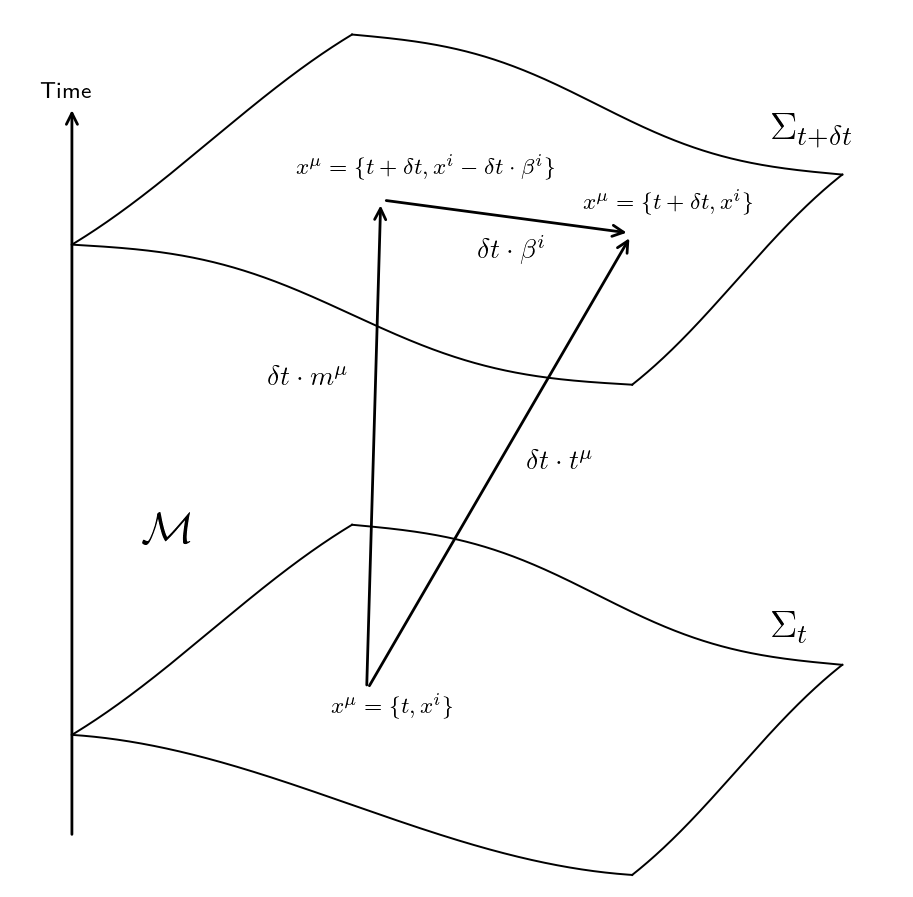
\includegraphics[width=0.65\textwidth]{png/ADM_screeny.png}
    \caption{An illustration of two hypersurfaces $\Sigma_t$ and $\Sigma_{t+\delta}$ and how they are connected by $m^\mu$. As can be seen, integral curves of $t^\mu$ have constant spatial coordinates $x^i$.  }
\end{figure}
There is a large gauge freedom associated with picking coordinates in general relativity; we choose to use a level set of the time coordinate $x^0=t$ to define our foliation hypersurfaces $\Sigma_t$. The other three coordinates $x^i$ for $i\in[1,2,3]$ can be used to span each hypersurface $\Sigma_t$ however we define. It is conventional to split the normal evolution vector $m^\mu$ into time $t^\mu$ and space parts $\beta^\mu$,
\begin{align}
\label{nr:eq:tmu} t^\mu &= \left( 1,0,0,0\right), \\
\label{nr:eq:betamu} \beta^\mu &= \left( 0,\beta^1,\beta^2,\beta^3\right),
\end{align}
such that,
\begin{align}
\label{nr:eq:m1} m^\mu &= t^\mu - \beta^\mu  = (\partial_0)^\mu - \beta^i (\partial_i)^\mu, \\
\label{nr:eq:m2} m^\mu &= \left( 1,-\beta^1,-\beta^2,-\beta^3\right).
\end{align}
We can view $t^\mu$ as the (not necessarily causal) worldline for a simulation gridpoint, hence we would like to evolve our PDEs along $t^\mu$ on a computer. In other words, integral curves of $t^\mu$ must have constant spatial coordinates on $\Sigma_t$. Equation~(\ref{nr:eq:m2}), along with the definitions $\bs{m} = \alpha \bs{n}$ and $\bs{n}^2=-1$, specifies $n^\mu$ and $n_\mu$,
\begin{align}
n^\mu &=  \frac{1}{\alpha}\left( 1,-\beta^1,-\beta^2,-\beta^3\right),\\
n_\mu &= -\alpha\left( 1,0,0,0\right).
\end{align}
The decomposed metric can be calculated, using the property that $\bs{\beta}$ is tangent to $\Sigma_t$ and orthogonal to $\bs{m}$,
\begin{align}
g_{00} &= \bs{g}(\bs{\partial}_0,\bs{\partial}_0) = \bs{g}(\bs{m} + \beta^i \bs{\partial}_i,\bs{m} + \beta^j\bs{\partial}_j) = \bs{g}(\bs{m},\bs{m}) + \beta^i \beta_j \langle \bs{\partial}_i,{\bs{\mathrm{d}}} \bs{x}^j \rangle = -\alpha^2 + \beta^i \beta_i ,\\
 g_{0i} &= \bs{g} (\bs{\partial}_0,\bs{\partial}_i) =  \bs{g}(\bs{m} + \beta^j \bs{\partial}_j, \bs{\partial}_i) =   \beta^j\bs{g}( \bs{\partial}_j, \bs{\partial}_i) = \beta_i,\\
 g_{ij} &= \bs{g}(\bs{\partial}_i,\bs{\partial}_j) = \bs{\gamma}(\bs{\partial}_i,\bs{\partial}_j) = \gamma_{ij}.
 \end{align}
This is commonly called the $3+1$ Arnowitt-Deser-Misner (ADM) metric and $\alpha$, $\beta^i$ are referred to as the lapse and shift vector in this context. The line element and metric are commonly written as,
\begin{align}
\dd s^2 &= -\alpha^2 \dd t^2 + \gamma_{ij}\left[\dd x^i + \beta^i \dd t\right]\left[\dd x^j + \beta^j \dd t\right],\\
 g_{\mu\nu} &= \begin{pmatrix} -\alpha^2 + \beta^i \beta_i & \beta_i \\ \beta_j & \gamma_{ij} \end{pmatrix},\label{nr:eq:admmetric}\\
  g^{\mu\nu} &= \frac{1}{\alpha^2}\begin{pmatrix} -1  & \beta^i \\ \beta^j & \alpha^2\gamma^{ij} - \beta^i \beta^j \end{pmatrix},
 \end{align}
and using Cramer's rule for metric determinant,
\begin{equation} g^{00} = \frac{\det{\gamma_{ij}}}{\det{g_{\mu\nu}}},\end{equation}
we get the important relationship,
\begin{equation} \sqrt{-g} = \alpha \sqrt{\gamma} ,\label{nr:eq:gay}\end{equation}
where $g$ and $\gamma$ are the determinants of $g_{\mu\nu}$ and $\gamma_{ij}$ respectively.

\subsection{ADM Equations} \label{nr:sec:ADM}
Now that we have some coordinates suitable for the spacetime foliation we can find the Arnowitt-Deser-Misner (ADM) evolution equations for $\K_{ij}$ and $\gamma_{ij}$. First we simplify the Lie derivative $\L_t$ along $t^\mu$ using,
\begin{equation}
\L_t \bs{T} = \partial_t \bs{T},
\end{equation}
for any tensor $\bs{T}$ as $\partial_\nu t^\mu=0$. This can be used to expand the Lie derivative along $m^\mu$,
\begin{equation} \L_m = \L_{t} - \L_\beta  = \partial_t - \L_\beta,\end{equation}
and the ADM equations can be written by substituting $\L_m\rightarrow \partial_t - \L_\beta$ in the normal evolution equations in section \ref{nr:sec:einsteindecomp} for $\bs{\K}$ and $\bs{\gamma}$. The ADM equations are,
\begin{align}
\partial_t \K_{ij} &= \L_\beta \K_{ij}  -\D_j\D_i \alpha + \alpha \left[ \R_{ij} + \K\K_{ij} - 2\K^k_i\K_{kj} + 4\pi \left[ \gamma_{ij}\left[ \S-\rho\right]-2\S_{ij}\right]\right],\\
\partial_t \gamma_{ij} &= \L_\beta \gamma_{ij} - 2\alpha\K_{ij}.\end{align}
Unfortunately, these PDEs turn out to be an ill-posed initial value problem with typical gauges \cite{frittelli2000ill}; this means that the time evolution of these equations does not generally depend smoothly on the initial data.


\subsection{BSSN} \label{nr:sec:bssn}
To tackle the ill-posedness of the ADM equations in section \ref{nr:sec:ADM} we
now discuss the Baumgarte-Shapiro-Shibata-Nakamura (BSSN) formalism \cite{Baumgarte:1998te}
The first step in BSSN is to decompose the 3-metric into the conformal metric
$\tilde{\gamma}_{ij}$ and the conformal factor $\chi$,
\begin{align}
\tilde{\gamma}_{ij} &= \chi \gamma_{ij},\\
 \det{\tilde{\gamma}_{ij}} &= \tilde{\gamma} = \chi^3\gamma = 1,
\end{align}
with the above being the convention used in {\sc GRChombo} described in section
\ref{grchombo:sec:grchombo}. Other conventions include factors such as
$\tilde{\gamma}_{ij} = \psi^{-4}\gamma_{ij}$ or $\tilde{\gamma}_{ij} =e^{-\phi}\gamma_{ij}$.
Along with this the extrinsic curvature $\K_{ij}$ is conformally decomposed with
$\chi$ and modified to be trace free,
\begin{equation}
\tilde{A}_{ij} = \chi\left[ \K_{ij}-\frac{1}{3}\K\gamma_{ij}\right],
 \end{equation}
 so that $\tilde{A}_{ij}\gamma^{ij}=0$.
During an evolution the algebraic constraint $\trace{\tilde{A}_{ij}=0}$ (and sometimes
$\tilde{\gamma}=1$) is enforced which avoids the undesirable growth of numerical error
\cite{Gundlach:2006tw,Cao:2011fu}.
As discussed later in
section \ref{nr:sec:gaugeconditions}, the definition of $\chi = \gamma^{-1/3}$
is good for black hole simulations where $\gamma\rightarrow\infty$ but $\chi
\rightarrow 0$. For example the isotropic Schwarzschild metric has,
\begin{align}
\gamma &= \left[ 1+ \frac{M}{2r}\right]^{12},\\
\chi &=\left[ \frac{r}{\frac{M}{2} + r}\right]^4.
\end{align}

The next step is to introduce the conformal connection functions as auxiliary variables,
\begin{align}
 \tilde{\Upsilon}^i_{\,\;jk} &= \frac{1}{2}\tilde{\gamma}^{il}\left[ \partial_j \tilde{\gamma}_{kl} + \partial_k \tilde{\gamma}_{lj} - \partial_l \tilde{\gamma}_{jk}\right] = \Upsilon^i_{\;\,jk} + \left[ \delta^i_j \partial_k + \delta^i_k \partial_j - \gamma^{il}\gamma_{jk}\partial_l\right] \ln \sqrt{\chi},\\
 \tilde{\Upsilon}^i &= \tilde{\gamma}^{jk}\tilde{\Upsilon}^i_{\,\;jk} = -\partial_i \tilde{\gamma}^{ij},
 \end{align}
where $\Gamma^i_{\,\,\,jk}$ are the Christoffel symbols of $\Sigma_t$ as shown
in Eq.~(\ref{nr:eq:3connection});
this reduces the set of vacuum evolution variables to $\{\chi,\tilde{\gamma}_{ij},
\K,\tilde{\A}_{ij},\tilde{\Upsilon}^i \}$. The idea behind introducing the $\tilde{\Upsilon}^i$ is that
their derivatives ($\partial_j\tilde{\Upsilon}^i$) encode second derivatives of the metric
that ruin strong hyperbolicity in the ADM equations; instead these offending terms are
encoded as first derivatives of a new evolution variable and are removed from the principal symbol governing the
hyperbolicity of the equations. It is conventional to use $-\partial_i
\tilde{\gamma}^{ij}$ to evaluate the conformal connection coefficients when they
appear in the RHS of an equation, but $\partial_j \tilde{\Upsilon}^i$ is calculated
by differentiating the evolution variable $\tilde{\Upsilon}^i$.

One final detail, not mentioned in the Z4 and CCZ4 formulations discussed
later, is the addition of multiples of the Hamiltonian and Momentum
constraint equations (in section
\ref{nr:sec:einsteindecomp}) to the evolution equations to change the
characteristic matrix and improve stability. This is not always necessary and
can depend on the gauge used, for more information see \cite{Gundlach:2004jp}.

The BSSN formalism is not the only way to find a well-posed set of evolution
equations for general relativity. Another strongly hyperbolic formalism is the
generalised harmonic gauge \cite{Garfinkle:2001ni,garfinkle2002harmonic,Pretorius:2004jg,Pretorius:2005gq} with,
\begin{equation}\Box x^\mu = H^\mu,\end{equation}
for some functions $H^\mu$.


\subsection{Z4 Formalism}
The Z4 formalism \cite{gundlach2005constraint} generalises the Einstein equation
to include an unphysical field $Z_\mu$, along with damping terms parameterised by
$\kappa_1$, $\kappa_2$,
\begin{equation}
\label{nr:eq:z4einstein} R_{\mu\nu} + \nabla_\mu Z_\nu +
\nabla_\nu Z_\mu - \kappa_1\left[ n_\mu Z_\nu + n_\nu Z_\mu -
[1+\kappa_2]g_{\mu\nu}n^\alpha Z_\alpha\right] = 8\pi G \left[T_{\mu\nu}-
\frac{1}{2}Tg_{\mu\nu} \right].
\end{equation}
Of course regular General Relativity is recovered by setting $Z_\mu=0$. It can
be shown that achieving $Z_\mu=0$ whilst dynamically evolving $Z_\mu$  is
equivalent to solving the constraints. Taking the divergence of
the trace reverse of Eq.~(\ref{nr:eq:z4einstein}),
and noting that both $G_{\mu\nu}$ and $T_{\mu\nu}$ are divergenceless, gives
\begin{equation}
\nabla^\nu \nabla_\nu Z_\mu  + R_{\mu\nu}Z^\nu = -\kappa_1 \nabla^\nu
\left( n_\mu Z_\nu + n_\nu Z_\mu + \kappa_2 g_{\mu\nu} n^\alpha Z_\alpha\right).
\end{equation}
$Z_\mu$ is subjected to a wave equation,
transporting constraint violation off the computational domain. It can be shown
that the system is driven to $Z_\mu =0$ for $k_1>0$ and $k_2>-1$. It is much
cheaper to evolve the variables $Z_\mu$, driven to zero, than to solve four
elliptic PDEs for the constraints $\{\mathcal{H},\M^i\}$ on each timestep.


\subsection{CCZ4} \label{nr:sec:ccz4}
Merging the conformal decomposition of the BSSN formalism with the constraint damping Z4 formalism leads to
Z4c formalism \cite{Bernuzzi:2009ex} and the conformal covariant Z4 (CCZ4) formalism.
The purpose of this is to get a formalism combining the strong hyperbolicity
of the BSSN equations and the constraint damping effects of the Z4 system.
In this thesis
we will use the CCZ4 formalism which employs the additional modifications,
\begin{align} \Theta &= -n\cdot Z  = -\alpha Z^0,\\
\hat{\Upsilon}^i &= \tilde{\Upsilon}^i + \frac{2\gamma^{ij}Z_j}{\chi},\end{align}
leaving us with the following set of vacuum evolution variables
$\{\chi, \tilde{\gamma}_{ij},\K,\tilde{\A}_{ij},\hat{\Upsilon}^i,\Theta \}$.
The evolution equations can now
be found in the CCZ4 scheme by applying a 3+1 decomposition to the Z4 modified
Einstein equation~(\ref{nr:eq:z4einstein}) and proceding as in the BSSN formalism.
To illustrate this, we derive the equation of motion for $\chi$ in the CCZ4 formalism.
Using Eqs.~(\ref{intro:eq:mdmmdm}) and (\ref{nr:eq:Lmgamma}) with $\chi^{-3}=\gamma$
we obtain,
\begin{align}
\L_m {\gamma} = \gamma \gamma^{ij} \L_m \gamma_{ij} = -2 \gamma \alpha \gamma^{ij} \K_{ij} = -2\gamma \alpha \K.
\end{align}
This can be used to simplify the Lie derivative of $\chi$,
\begin{align}
\L_m \chi &= \L_{\partial_t}\chi - \L_\beta \chi,\\
 &= (\partial_t)^i \partial_i \chi + \omega \chi \partial_i (\partial_t)^i - \beta^i \partial_i \chi - \omega \chi \partial_i \beta^i ,\\
 &= \partial_t \chi - \beta^i \partial_i \chi +\frac{2}{3} \chi\partial_i \beta^i ,\\
\L_m \chi &= \L_m \gamma^{-\frac{1}{3}}  ,\\
&=-\frac{1}{3}\gamma^{-\frac{4}{3}}\L_m \gamma  ,\\
&=\frac{2}{3}\gamma^{-\frac{1}{3}} \alpha \K ,\\
&=\frac{2}{3}\chi \alpha \K ,
\end{align}
where Eq.~(\ref{intro:eq:Ltensordensity2}) has been used with $\bs{\mathcal{T}}=\chi$ as $\chi$ is a scalar density of weight $\omega=-2/3$. Re-arranging gives the equation of motion for $\chi$,
\begin{equation}
\partial_t \chi =  \beta^i \partial_i \chi + \frac{2\chi}{3} \left[\alpha \K - \partial_i \beta^i \right].
\end{equation}
A similar process returns the remaining CCZ4 equations but care should be taken to include the Z4 terms ($\Theta,\hat{\Upsilon}^i$) where they are needed. The complete list of CCZ4 equations used in simulations with {\sc GRChombo} (section \ref{grchombo:sec:grchombo}) are given below:
\begin{align} \partial_t \chi &=  \beta^i \partial_i \chi + \frac{2\chi}{3} \left[\alpha \K - \partial_i \beta^i \right],\\
\partial_t\tilde{\gamma}_{ij} &=  \beta^k\partial_k\tilde{\gamma}_{ij}  + \tilde{\gamma}_{kj}\partial_i \beta^k + \tilde{\gamma}_{ik}\partial_j\beta^k - \frac{2}{3}\tilde{\gamma}_{ij} \partial_k \beta^k - 2\alpha\tilde{\A}_{ij},\\
\partial_t\K &=  \beta^k\partial_k\K + \alpha\left[ \R + 2\bs{\D}\cdot \bs{Z} + \K\left[ \K-2\Theta\right]\right] - 3\alpha \kappa_1\left[ 1+\kappa_2\right]\Theta \nonumber\\
&-\chi\tilde{\gamma}^{kl}\D_k\D_l\alpha + 4\pi G\alpha\left[ \S - 3\rho\right], \\
\partial_t\tilde{\A}_{ij} &=  \beta^k \partial_k \tilde{\A}_{ij}+\chi\left[\alpha\left[\R_{ij} + 2\D_{(i}Z_{j)}-8\pi G \S_{ij} \right] -\D_i\D_j\alpha \right]^{TF}\nonumber\\
& +\tilde{\A}_{ij}\left[ \alpha\left[ \K-2\Theta\right]-\frac{2}{3}\K^2\right] + 2\tilde{\A}_{k(i}\partial_{j)}\beta^k -2\alpha\tilde{\gamma}^{kl}\tilde{\A}_{ik}\tilde{\A}_{lj},\\
\partial_t\Theta &= \beta^k\partial_k \Theta + \frac{1}{2}\alpha\left[ \R + 2\bs{\D}\cdot \bs{Z} - \tilde{\A}_{kl} \tilde{\A}^{kl} + \frac{2}{3}\K^2 - 2\Theta\K\right] -\kappa_1\alpha\Theta\left[ 2+\kappa_2\right] - Z^k\partial_k\alpha - 8\pi G \alpha \rho, \\
\partial_t\hat{\Upsilon}^i &=  \beta^k \partial_k \hat{\Upsilon}^i + \frac{2}{3}\left[ \partial_k \beta^k \left[ \tilde{\Upsilon}^i+2\kappa_3 \frac{Z^{i}}{\chi}\right]-2\alpha\K\frac{Z^j}{\chi}\right]-2\alpha\kappa_1\frac{Z^i}{\chi}\nonumber \\
& + 2\tilde{\gamma}^{ij}\left[ \alpha\partial_j\Theta -\Theta \partial_j\alpha \right] -2\tilde{\A}^{ij}\partial_j\alpha - \alpha\left[ \frac{4}{3}\tilde{\gamma}^{ij}\partial_j\K + 3\tilde{\A}^{ij}\frac{\partial_j \chi}{\chi}\right]\nonumber\\
& -\left[ \tilde{\Upsilon}^j + 2\kappa_3 \frac{Z^j}{\chi}\right]\partial_j \beta^i + 2\alpha \tilde{\Upsilon}^i_{\,\,\,jk}\tilde{\A}^{jk} + \tilde{\gamma}^{jk}\partial_j\partial_k \beta^i + \frac{1}{3} \tilde{\gamma}^{ij}\partial_k \partial_j \beta^k - 16\pi G \alpha \tilde{\gamma}^{ij}\S_j, \\
\partial_t \vp &= \beta^k\partial_k \vp - \alpha\Pi ,\label{nr:eq:ccz4kg1}.\end{align}
In the CCZ4 equations there is an additional parameter $\kappa_3$ premultiplying terms in the evolution of $\hat{\Upsilon}^i$ which experimentally were found to lead to instabilities in black hole simulations \cite{PhysRevD.85.064040}; setting $\kappa_3<1$ stabilises the simulation but at the cost of covariance. Later on it was realised that setting $\kappa_3=1$ and $\alpha\kappa_1\rightarrow\kappa_1$ retains covariance as well as numerical stability \cite{Alic:2013xsa}; in this work $\kappa_1=0.1$, $\kappa_2=0$ and $\kappa_3=1$ is used. Notably the pair of variables $\R_{ij} + \D_{(i}Z_{j)}$, and its traced version
$\R + \bs{\D}\cdot \bs{Z}$, always appear together; separately they would ruin
strong hyperbolicity but together they do not.


The CCZ4 scheme proves several benefits.
\begin{itemize}
\item Any initial data that does not satisfy the constraints will generally not do so during evolution when using the BSSN formalism either. Given that superposition of solutions in GR does not generally give a new solution, but does approximate one for separated compact objects, all the simulated binaries considered in this work will have non constraint satisfying initial data.
\item Constraint satisfying initial data can also develop constraint violation over time; one reason being that finite resolution imposes some small deviation from the continuum solution. More importantly, the use of adaptive mesh refinement (discussed in section \ref{grchombo:sec:grchombo}) introduces interpolation errors into the simulation at the boundary of the different grid resolution levels. The use of the CCZ4 scheme can also help to reduce the constraint violation generated in this way.
\item Sommerfeld boundary conditions (discussed in section \ref{grchombo:sec:sommerfeld}) used are inexact in GR and will introduce errors at the outer boundary that ruin constraint satisfaction and in the worst case scenario cause a simulation to crash. Again, the CCZ4 scheme can be used to help combat this.
\end{itemize}
In all the cases above, the CCZ4 system forces the evolution towards constraint satisfaction, despite the numerical errors and approximations. There is a caveat, even if a simulation satisfies the constraints, there is no guarantee it is the desired solution to Einstein's equation. Additionally, the damping is more efficient for small amplitude and high frequency errors.



\subsection{Gauge Conditions}\label{nr:sec:gaugeconditions}

The lapse $\alpha$ and shift $\beta^i$ are freely specifiable on a hypersurface
$\Sigma_t$ being gauge variables, however they must be chosen carefully along with
a suitable initial Cauchy surface $\Sigma_{t_0}$ and initial data. $\Sigma_{t_0}$
should be a smooth non-intersecting Cauchy surface as described in section
\ref{nr:sec:foliation} and contain smooth initial data. It is also wise to avoid
singularities (both coordinate and physical) on this surface. As an example,
consider the simulation of a single Schwarzschild black hole.
Figure~\ref{nr:fig:eddington-finkelstein} (left) shows how an initial data
surface could extend to the singularity if polar-areal coordinates are used.
Figure~\ref{nr:fig:eddington-finkelstein} also shows how the physical singularity
is avoided when using isotropic coordinates. In this work the isotropic gauge is
used; not only does this provide an initial Cauchy surface free of physical
singularities but also allows for trivial swapping between spherical polar and
Cartesian (used in simulations) coordinates. However, for a poor choice of
lapse function, even a well chosen $\Sigma_{t_0}$ can advance to the physical
singularity in finite simulation time.  For a comprehensive introduction to gauge
conditions the reader is directed to
\cite{baumgarte_shapiro_2010,alcubierre2008introduction,gourgoulhon20073+}.

%   \begin{figure}[h]
%   \caption{Penrose Diagrams, $\Sigma_{t_0}$ dashed, Left: Ingoing Eddington-Finkelstein Coordinates, Right: Isotropic Coordinates.}
%   \centering
%   \subfloat{\includegraphics[width=0.43\textwidth]{schwarzschild2.png}\label{boson:fig:f1}} \label{nr:fig:eddington-finkelstein}
%   \hfill
%   \subfloat{\includegraphics[width=0.5\textwidth]{schwarzschild.png}\label{boson:fig:f2}} \label{nr:fig:isotropic}
% \end{figure}

  \begin{figure}[h]
  \caption{Penrose Diagram of the maximally extended Schwarzschild spacetime; the top (future) squiggle represents the spacelike black hole singulary and the bottom (past) squiggle represents the white hole singularity. In the right hand diagram, the straight dashed line labelled by $\Sigma_{\rm iso}$ represent the initial hypersurface $\Sigma_{t_0}$ for $t=0$ in isotropic coordinates. In the left hand diagram, the dashed line labelled by $\Sigma_{\rm pa}$ represent the initial hypersurface $\Sigma_{t_0}$ for $t=0$ in polar-areal coordinates. Notably $\Sigma_{\rm pa}$ initially touches the physical singularity whereas $\Sigma_{t_0}$ does not; additionally $\Sigma_{\rm pa}$ is not a Cauchy surface as there exist causal curves which can intersect it multiple times.}
  \centering
  \subfloat{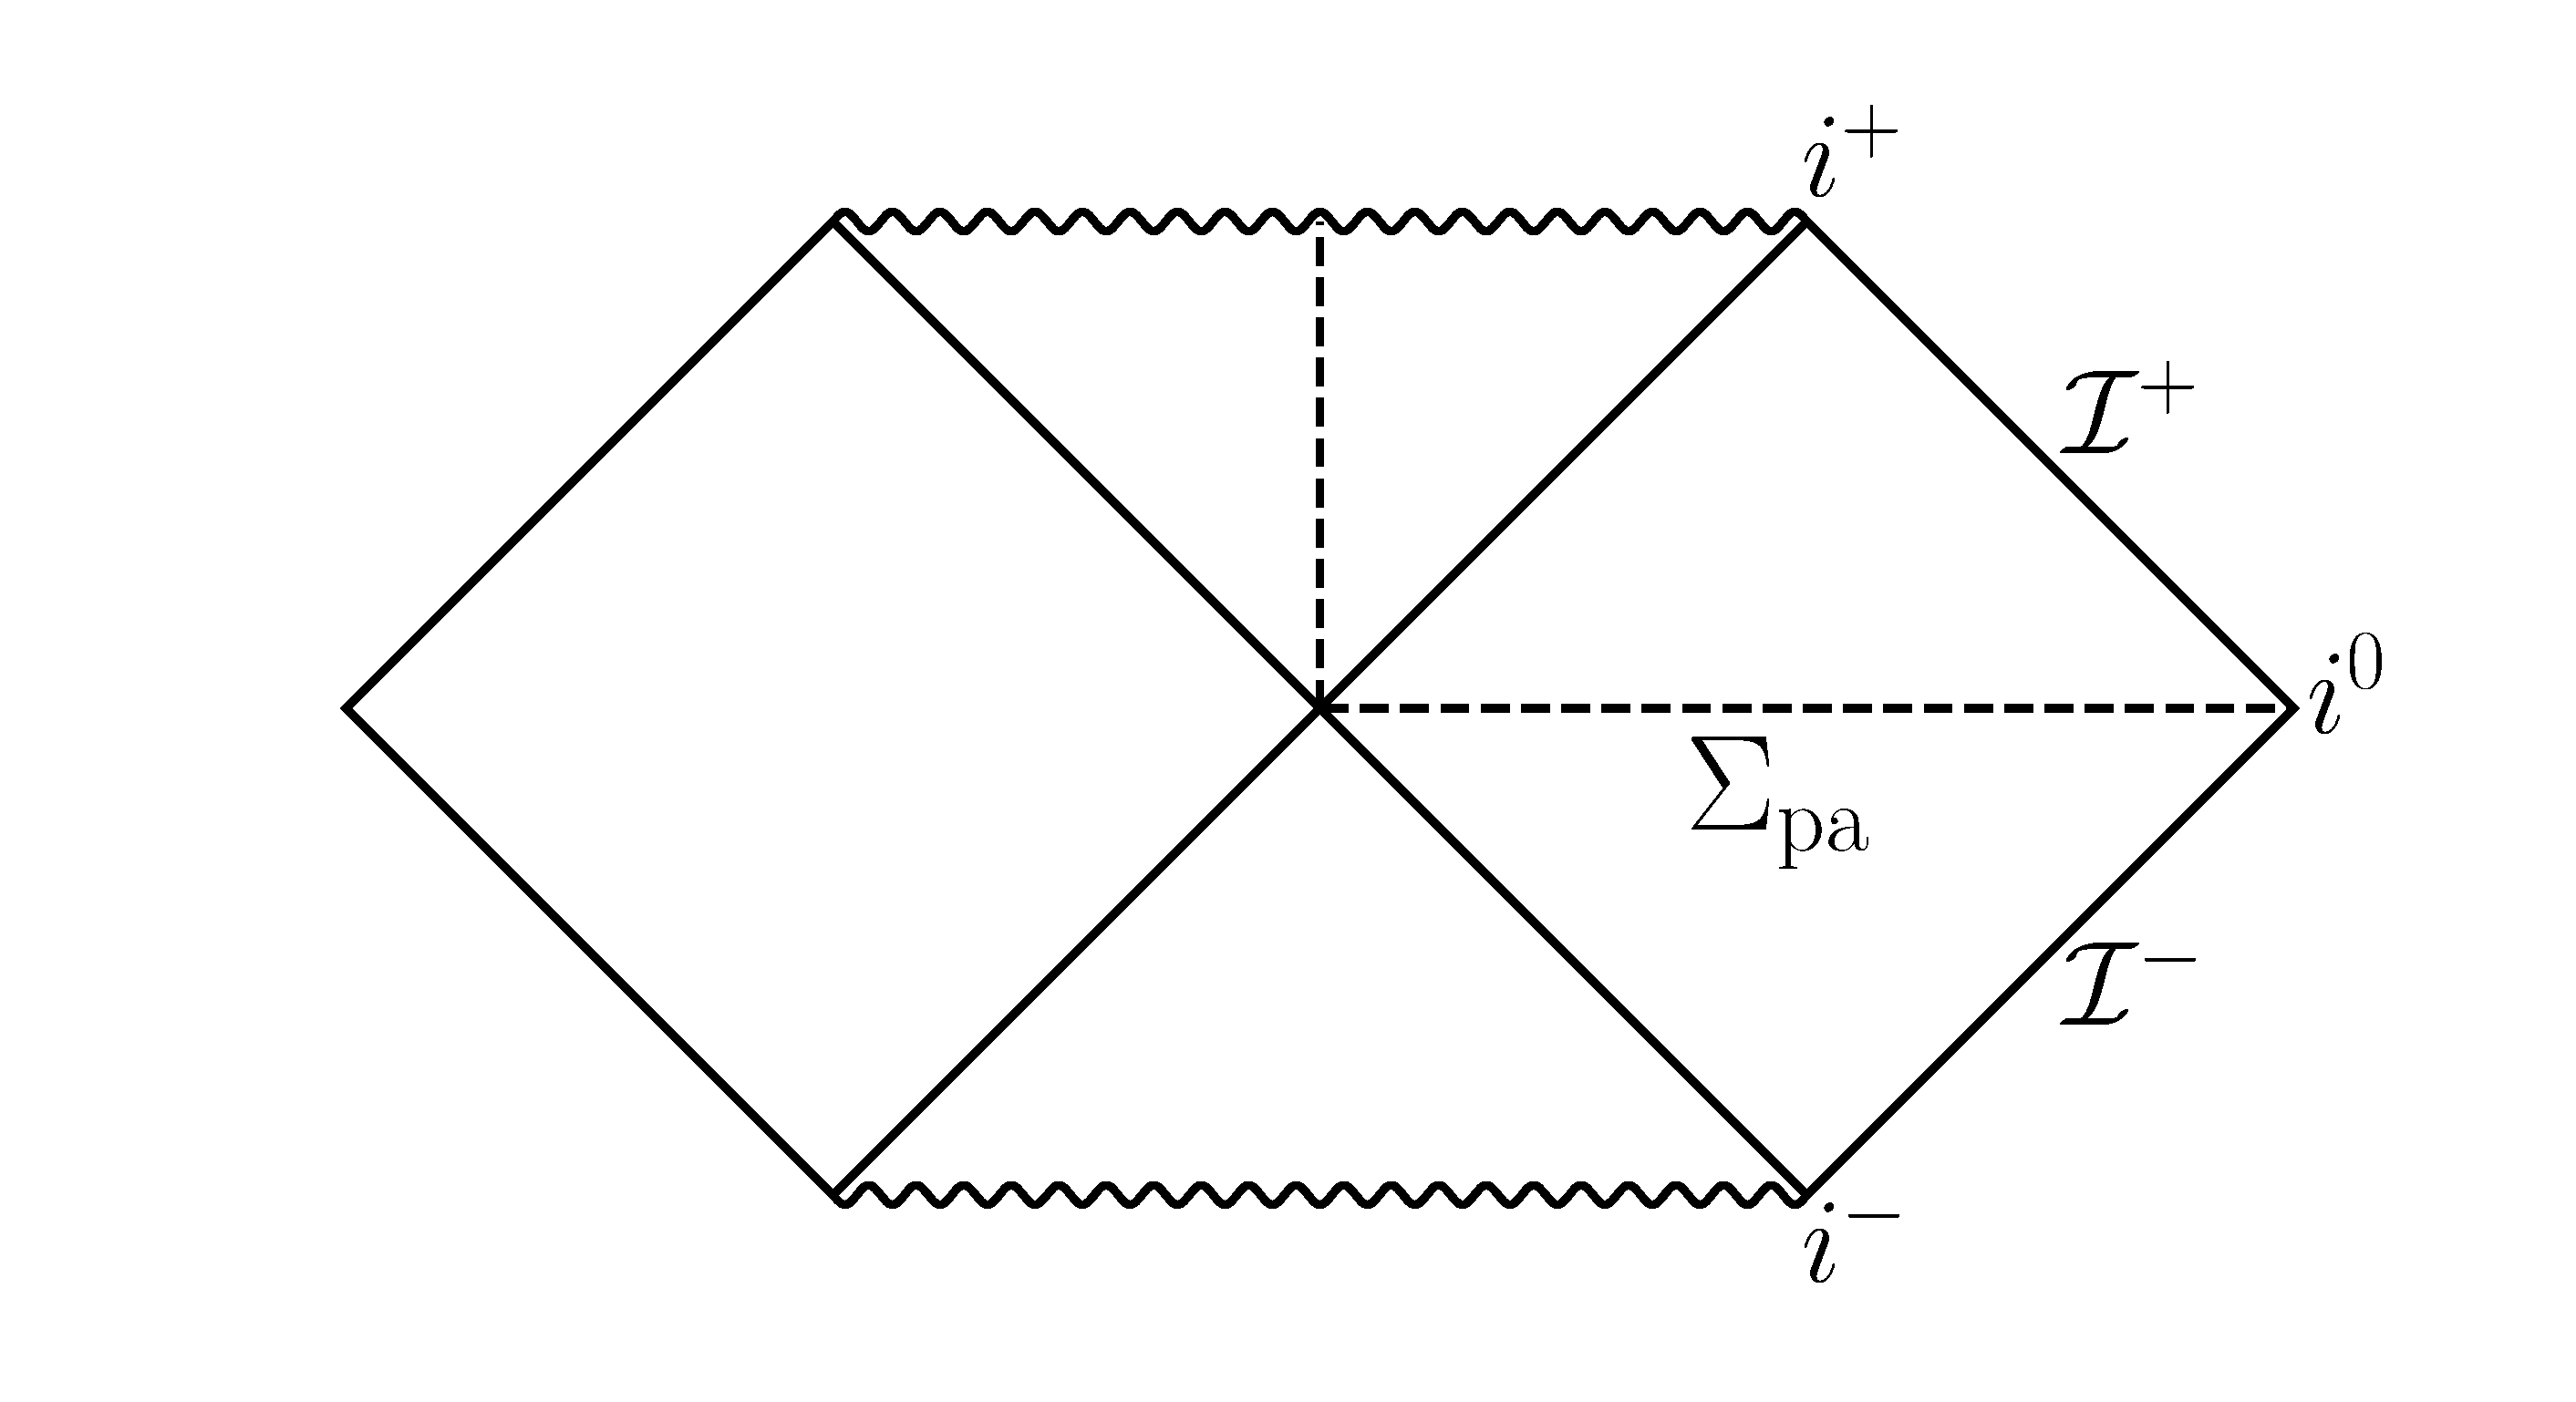
\includegraphics[width=0.50\textwidth]{png/penrose_sc.pdf}} \hfill
  \subfloat{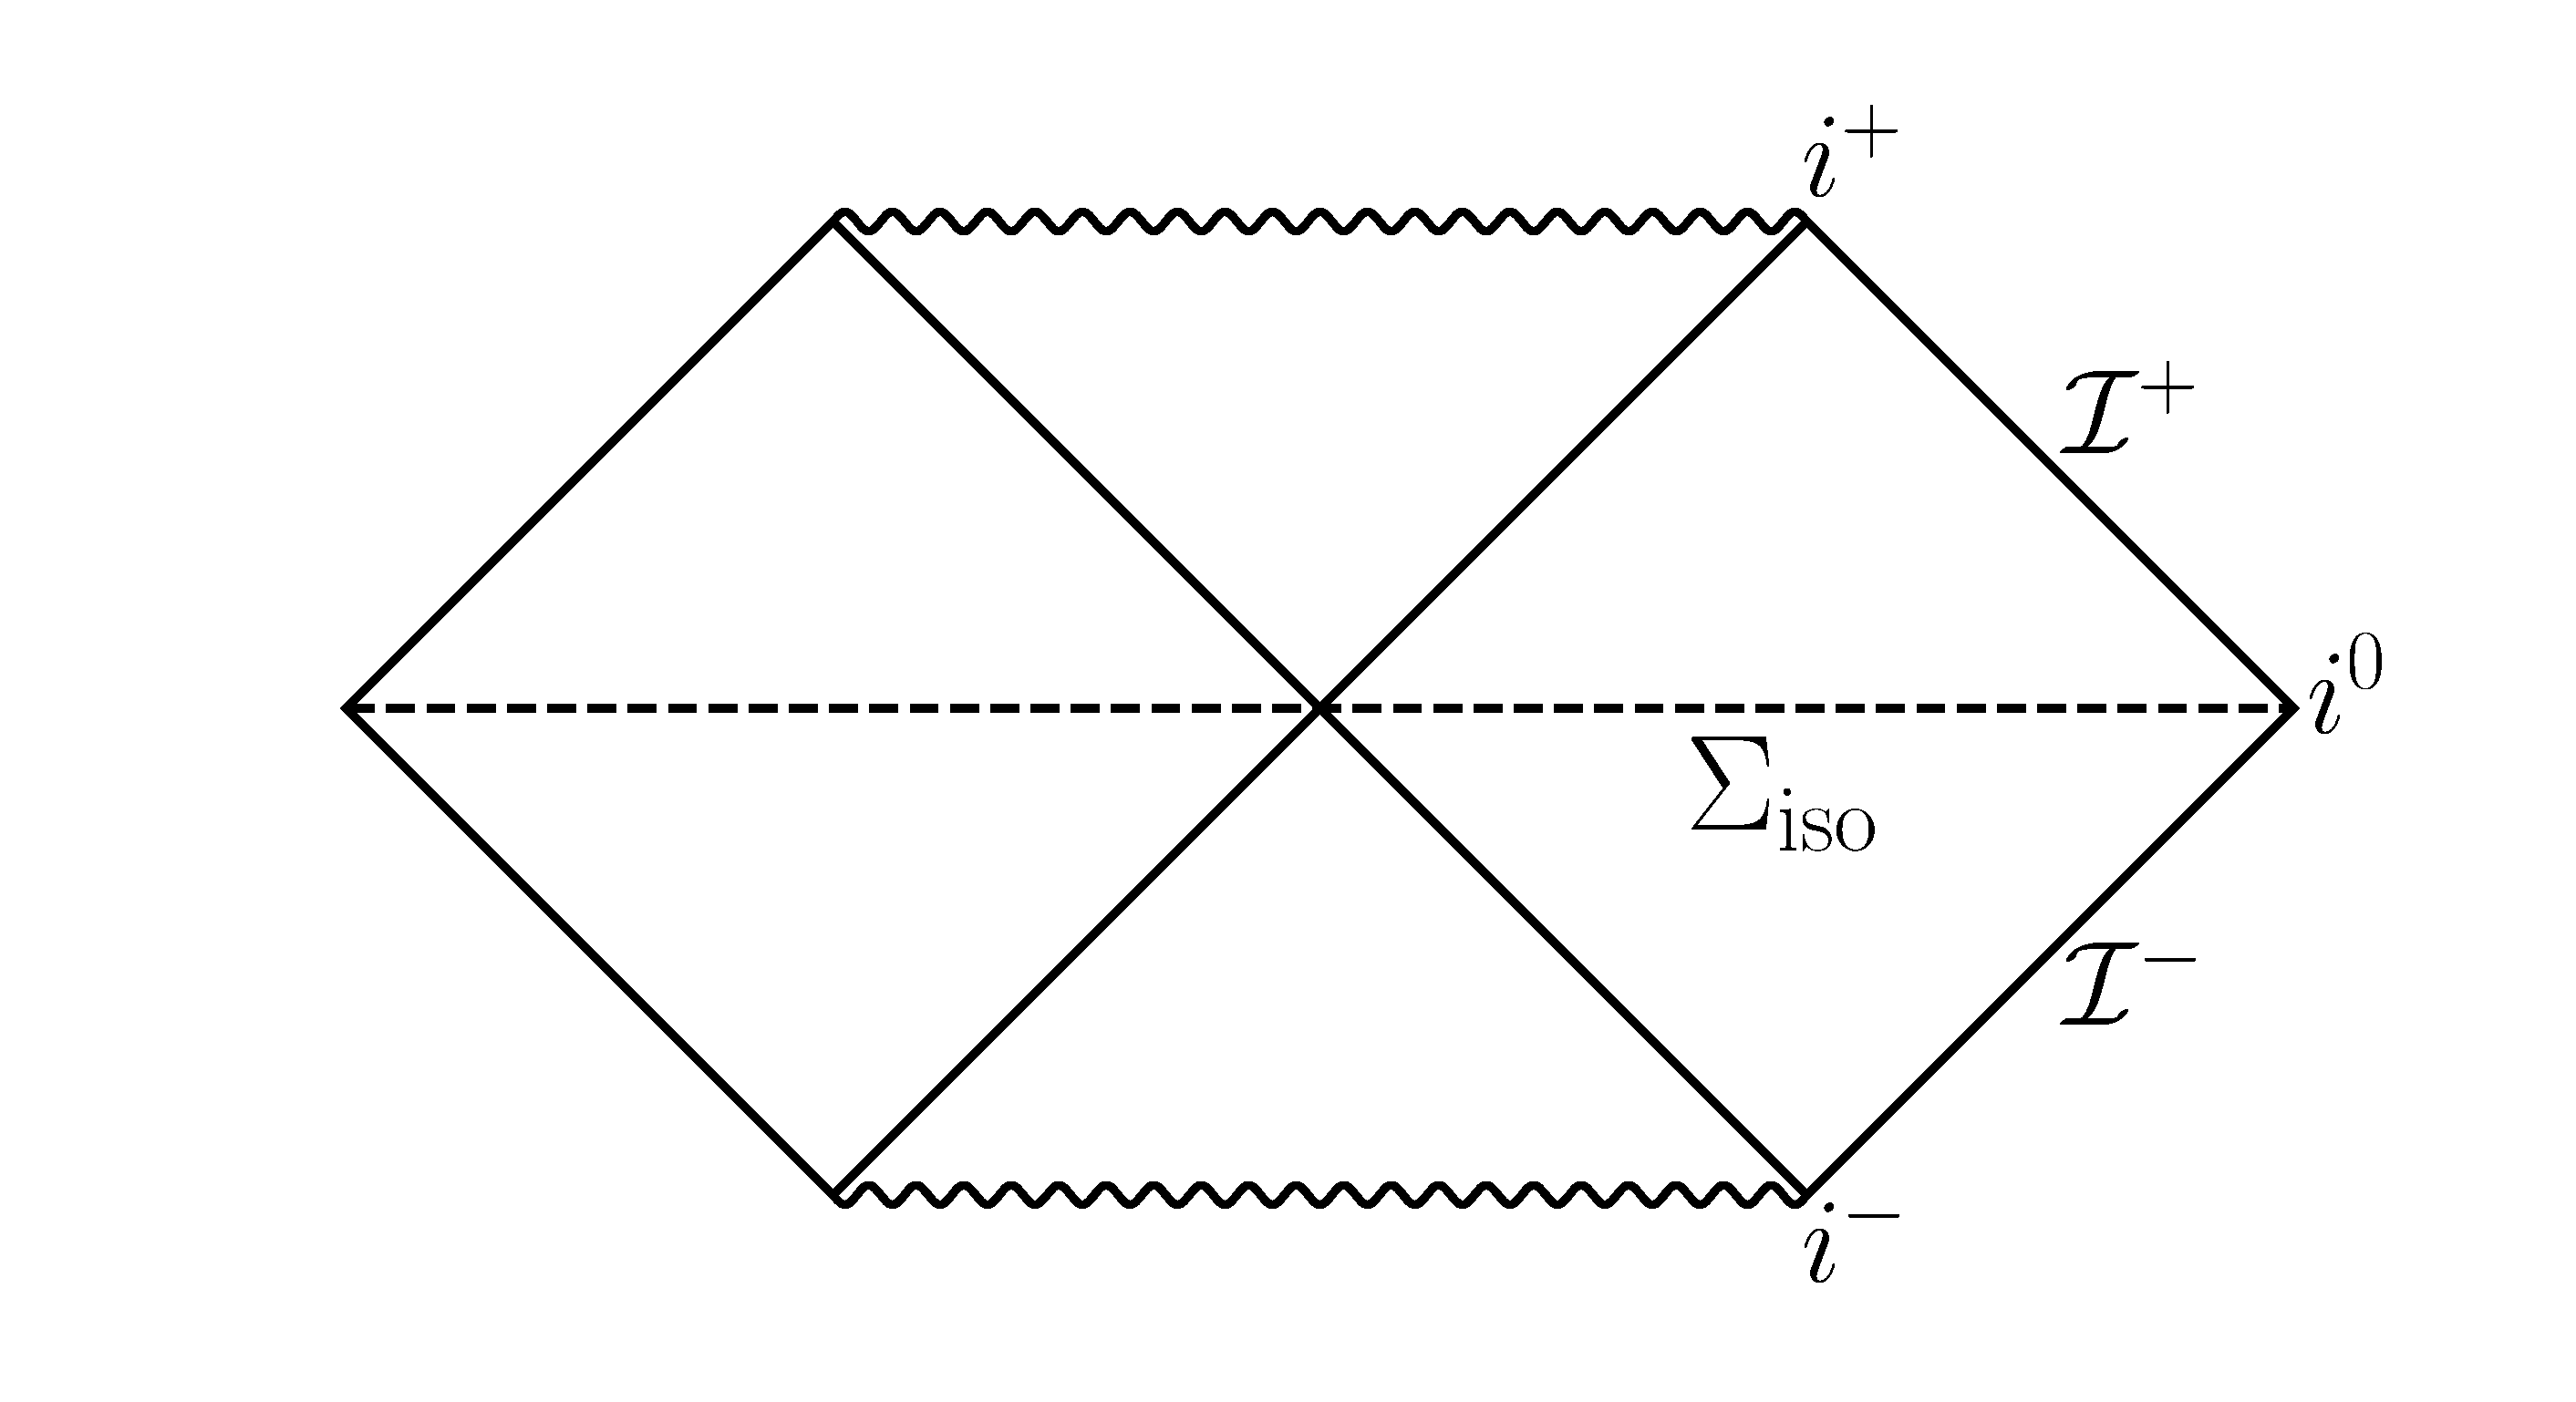
\includegraphics[width=0.50\textwidth]{png/penrose_iso.pdf}}
  \label{nr:fig:eddington-finkelstein}\label{nr:fig:isotropic}\label{boson:fig:f1}
\end{figure}

\subsubsection{Lapse Slicing Conditions}

The simplest lapse choice would be to enforce $\alpha=1$, called geodesic slicing, with the hypersurface following integral curves of $n^\mu$; given that geodesics can converge this can lead to hypersurface self-intersection which breaks the definition of a Cauchy surface and the simulation will likely fail. Another problem is that a black hole singularity can be reached in finite simulation time.

An alternative slicing condition is the maximal slicing condition which keeps the volume element $\sqrt{-g}$ constant along geodesics. This means as $\gamma\rightarrow\infty$ nearing a singularity $\alpha\rightarrow0$ from Eq.~(\ref{nr:eq:gay}), causing the hypersurface to advance more slowly before a singularity is reached as demonstrated in Fig.~(\ref{nr:fig:singularity_avoiding}). This property is called singularity avoiding and is crucial for numerical stability unless using excision\footnote{Excision is the practice of cutting singularities out of the computational domain while supplying suitable boundary conditions about the excised region}. Maximal slicing can be implemented by forcing $\mathcal{K} = \partial_t \K = 0\,\forall \,t$ which requires a slow elliptic solve for $\alpha$ at each timestep. Instead of performing this slow elliptic solve, $\alpha$ is promoted to an evolution variable and is evolved along with every other simulation variable. To do this we can pick an algebraic slicing condition of the Bona-Masso type,
\begin{equation}\L_m \alpha = \partial_t \alpha - \beta^i \partial_i \alpha = -\alpha^2 f(\alpha)\K. \end{equation}
Using this with $f = 2\alpha^{-1}$ gives,
\begin{equation}\L_m \alpha = \partial_t \alpha - \beta^i \partial_i \alpha = -2\alpha \K, \label{nr:eq:1pluslog} \end{equation}
which is called 1+log slicing; this is very common in Numerical Relativity codes. In practice 1+log slicing is strongly singularity avoiding reaching $\alpha=0$ before the singularity. This is modified in the CCZ4 scheme to,
\begin{equation}\partial_t \alpha = -2\alpha\left[ \K-2\Theta\right] + \beta^i \partial_i \alpha.\end{equation}
Using Gaussian normal coordinates $\beta^i=0$ and provided $\Theta=0$, the 1+log slicing condition reduces to,
\begin{equation} \alpha = 1+ \ln \gamma,\end{equation}
giving the slicing condition it's name \cite{alcubierre2008introduction}.

\begin{figure}[h!]
    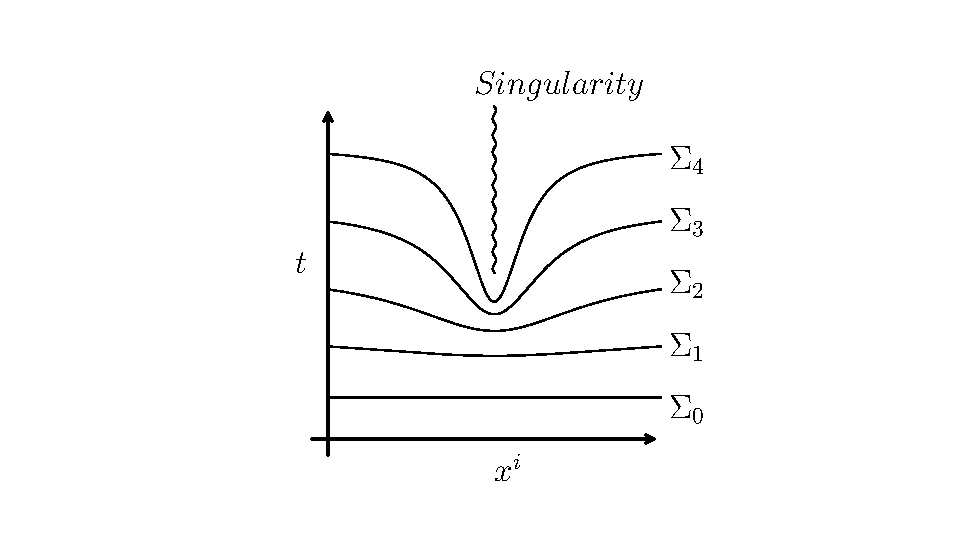
\includegraphics[width=0.9\textwidth]{png/slicing.pdf}
      \caption{Diagram showing the time evolution of a hypersurface using a singularity avoiding slicing condition. The vertical squiggled line represents a physical singularity that is formed at some point in spacetime, potentially from the collapse of matter to a black hole.} \label{nr:fig:singularity_avoiding}
\end{figure}


\subsubsection{Shift Conditions}

The simplest choice for the shift vector would be $\beta^i=0$ but this can cause great stretching and shearing of integral curves of $m^\mu$ in the neighbourhood of a singularity as in Fig.~(\ref{nr:fig:singularity_avoiding}); the effect of this is that neighbouring gridpoints may have large differences in field values leading to inaccurate and unstable evolutions.

 Another negative side effect is that the computational domain can fall inside an event horizon in black hole simulations. To counteract this we want to employ a shift vector that minimises hypersurface shear $\sigma_{ij}$ which can be defined as \cite{smarr1978kinematical},
\begin{equation} \sigma_{ij}:= \perp^\mu_i \perp^\nu_j \left[\nabla_{(\mu} n_{\nu)}-\frac{1}{3}\gamma^{ab}\nabla_{(a} n_{b)} \gamma_{\mu\nu}\right], \end{equation}
where $\sigma_{ij}$ is tracefree corresponding to shearing rather than inflation or expansion. Minimising the total shear $\Sigma$,
\begin{equation} \Sigma = \int \sigma_{ij}\sigma^{ij}\sqrt{\gamma}\,\dd x^3,\end{equation}
with respect to $\beta^i$ leads to an elliptic PDE to be solved for each $\beta^i$ at each time step that minimises shear,
\begin{equation} \delta \Sigma = 0 \rightarrow \D_i\sigma^{ij}=0.\end{equation}
This is known as the minimal distortion shift condition. Promoting the $\beta^i$ to evolution variables is computationally cheaper than solving a set of PDEs at each time step. A very common choice is to promote the elliptic PDE for $\beta^i$ into a hyperbolic equation via introducing a $\partial_t^2\beta^i$ term and an artificial damping term parameterised by $\eta$. This becomes a damped wave equation and is supposed to transport away any part of $\beta^i$ which does not satisfy $\D_i \sigma^{ij}=0$. This works well with Sommerfeld (outgoing wave) boundary conditions given in section \ref{grchombo:sec:sommerfeld}. The standard Gamma driver shift condition is,
\begin{align}
\partial_t \beta^i &= FB^i,\label{nr:eq:gammadriver1}\\
 \partial_t B^i &= \partial_t \tilde{\Gamma}^i - \eta B^i,\label{nr:eq:gammadriver2}\end{align}
where $F=3/4$ and $\eta=1$ are used throughout this work.

\subsubsection{Moving Puncture Gauge}
The moving puncture gauge (MPG) is the combination of the 1+log slicing lapse condition
in Eq.~(\ref{nr:eq:1pluslog}) and the Gamma driver shift condition in
Eqs.~(\ref{nr:eq:gammadriver1}) and (\ref{nr:eq:gammadriver2}). In 2006, the
moving puncture gauge allowed for the first successful simulation of a black hole
binary \cite{PhysRevLett.96.111101} in the BSSN
formalism\footnote{It should be noted that a black-hole binary had been sucessfully
simulated before by \cite{Bruegmann:2003aw} in 2003 with co-rotating coordinates
and \cite{Pretorius:2005gq} in 2005 using the generalised harmonic gauge.} without
the use of excision. In 2012 the first simulations of black-hole binaries
using constraint damping schemes (in the MPG) such as CCZ4 \cite{alic2012conformal}
and Z4c \cite{Hilditch:2012fp} were achieved.
Although $\chi\rightarrow 0$, or $\gamma \rightarrow \infty$,
at the centre of a black hole, as long as a minimum value for $\chi$
(such as $\chi=10^{-4}$) is enforced a simulation can run. Even though it is
unphysical to modify a physical variable, the success of the MPG is often attributed
to the causal shielding\footnote{Errors that propagate at (or below) light speed
will be trapped by the event horizon. } provided by the
event horizon. Additionally, any extremely sharp field configurations produced will
be partially suppressed by a numerical dissipation scheme.

Not only does the MPG safeguard the divergence of fields at the puncture, but it allows the puncture to move; hence the name {\it moving} puncture gauge. Near the puncture, the lapse $\alpha$ becomes vanishingly small and the 1+log slicing condition in Eq.~(\ref{nr:eq:1pluslog}) becomes,
\begin{equation}
\partial_t \alpha = \beta^i \partial_i \alpha, \label{nr:eq:betavel}
\end{equation}
which causes the puncture to move. Assigning spatial coordinates $x^i_{\rm punc}(t)$ to the puncture, we know that
\begin{align}
\alpha(x^i_{\rm punc}) &= 0,\\
\frac{\dd}{\dd t} \alpha(x^i_{\rm punc})  &= \frac{\partial}{\partial t}\alpha + \left(\frac{\partial x^i}{\partial t}\Bigg|_{x^i=x^i_{\rm punc}}\right)\frac{\partial}{\partial x^i} \alpha =0,
\end{align}
which can be compared to Eq.~(\ref{nr:eq:betavel}) to show that
\begin{equation}
\beta^i = -\frac{\partial }{\partial t}x^i_{\rm punc}\,.
\end{equation}
This shows that the puncture must move along integral curves of $-\beta^i$.




%\newpage
%\pagenumbering{arabic}




\section{Mathematical Modelling of Boson Stars}
\subsection{The Action} \label{boson:sec:action}
The Boson Stars considered are a complex Klein Gordon Scalar field, $\varphi$, minimally coupled to gravity. The action is the Einstein-Hilbert vacuum action plus the matter action for curved space,
\begin{gather} S = \int_\mathcal{M}\left[\mathcal{L}_{EH} + \mathcal{L}_M\right] \sqrt{-g}\,\dd x^4, \\
 \L_{EH} = \frac{c^4}{16\pi G}R, \\
 \L_{M} =-\frac{1}{2}g^{\mu\nu}\nabla_\mu \bar{\varphi} \nabla_\nu \varphi - \frac{1}{2}V(|\varphi|^2),  \end{gather}
Here $V$ is the Klein-Gordon potential and it's effect on boson stars is discussed in \cite{Schunck:2003kk} \cite{Liebling:2012fv}. Some common choices of potentials are,
\begin{align}
V_{\rm mini} &= \frac{m^2 c^2}{\hbar^2 }|\vp|^2,\label{boson:eq:Vmini} \\
V_{\rm int} &= \frac{m^2 c^2}{\hbar^2 }|\vp|^2 + \frac{1}{2}\Lambda_4|\vp|^4 ,\\
V_{\rm soli} &= \frac{m^2 c^2}{\hbar^2 }|\vp|^2\left(1-\frac{|\vp|^2}{2\sigma^2}\right)^2 , \label{boson:eq:Vsoliton}
\end{align}
where $\hbar$ and $c$ are given for completeness but will be set to unity later.
Considering only the $m^2$ term, which corresponds to the squared mass of the particle in the quantum theory, we get a massive wave equation linear in $\varphi$, leading to so called {\it mini} Boson stars. Having $\Lambda_4\neq0$ gives {\it self-interacting} stars which have a nonlinear wave equation corresponding to particle creation and annihilation at the quantum level; self interacting potentials can include higher order terms in $\vp$ such as $|\vp|^6$, $|\vp|^8$ and more. These self interacting potentials tend to have star solutions with a higher density. Finally, Eq.~(\ref{boson:eq:Vsoliton}) describes the {\it solitonic} potential, giving rise to boson stars with compactness comparable to neutron stars. Solitonic boson stars and their gravitational
wave signatures have been studied in \cite{Palenzuela:2017kcg}.

Varying the action with respect to the metric and scalar field return the Einstein field equation and the Klein Gordon equation of curved space respectively,
\begin{align} R_{\mu\nu} - \frac{1}{2}R g_{\mu\nu} &=  \frac{8\pi G}{c^4} T_{\mu\nu}  ,\\
g^{\mu\nu}\nabla_\mu\nabla_\nu \vp &= \frac{\partial V}{\partial |\vp|^2}\vp .\label{boson:eq:KGeqn}\end{align}
Collectively these are known as the Einstein-Klein-Gordon (EKG) equations. From Eq.~(\ref{intro:eq:Tdef}), the boson-specific stress energy tensors are,
\begin{align}  
T_{\mu\nu} :&= -2\frac{\delta \mathcal{L}_{M}}{\delta g^{\mu\nu}}+g_{\mu\nu}\mathcal{L}_M, \\
T_{\mu\nu} &= \frac{1}{2}\nabla_{\mu}\bar{\varphi}\nabla_{\nu}\varphi+\frac{1}{2}\nabla_{\nu}\bar{\varphi}\nabla_{\mu}\varphi-\frac{1}{2}g_{\mu\nu}\left[g^{\alpha\beta}\nabla_\alpha\bar{\varphi}\nabla_\beta\varphi + V\right] \label{boson:eq:KGT}.
\end{align}
\subsubsection{Comparison of Boson Stars to Neutron Stars}
Boson stars differ greatly to neutron stars; studying neutron stars requires the fermionic, or ordinary fluid, stress tensor $\bs{T}_F$; 
\begin{equation} T^{\mu\nu}_F = \left[\rho c^2+ {P} \right]\frac{u^\mu u^\nu}{c^2} + P g^{\mu\nu} + 2u^{(\mu}q^{\nu)}+\pi^{\mu\nu}+ ...\,\,.\end{equation} 
The continuity equation from Eq.~(\ref{intro:eq:cont}), $\nabla_\nu T^{\mu\nu}=0 $, returns the highly nonlinear relativistic Navier-Stokes equations of curved space. The viscosity term $\pi^{\mu\nu}$ and heat flux $q^\mu$ are often omitted for simplicity. The remaining variables $\rho$, $P$ and $u^\mu$ are the fluid density, pressure and worldline tangent. Just as in flat space, the Navier-Stokes equations can develop shockwaves and the use of sophisticated shock capturing schemes is required, unlike the linear Klein-Gordon equation which is linear in the principal part.


\subsection{Solitons} \label{boson:sec:soliton}
A soliton is a wave packet that exhibits particle-like behaviour. More precisely, in classical field theory, a soliton
is a field or set of fields in a localised configuration that travels at constant speed without dispersing. This is a property of solutions to the linear wave equation but many solitonic solutions exist for non-linear differential equations as well. For
our purposes, we look for solitons in the Einstein-Klein-Gordon (EKG) system which are self gravitating
localised scalar field and metric configurations. In the case of the real scalar field it was shown that
there are no long lived solitons \cite{diez2013no}; however promoting the field to a complex scalar we can find a spherically
symmetric stationary soliton with the following configuration,
\begin{equation} \varphi = \Phi(r)e^{i\omega t}, \label{boson:eq:fieldansatz} \end{equation}
in spherical polar coordinates $x^\mu \in \{t,r,\theta,\phi \}$.
Traditionally, the polar areal gauge has been used for the metric's ansatz,
\begin{equation}g_{\mu\nu}\dd x^\mu \dd x^\nu =- a^2(r)\dd t^2 + b^2(r) \dd r^2 + r^2 \left[ \dd \theta^2 + \sin^2\theta \dd \phi^2\right],\label{boson:eq:polaransatz}\end{equation}
where the boundary condition $b^2(0)=1$ is demanded to avoid a conical singularity at the origin. However an isotropic gauge is more useful for simulations due to easier conversion to Cartesian space-coordinates, for more information on isotropic coordinates see section \ref{intro:sec:bh_theory}. The polar areal solution must then be transformed into an isotropic solution. Alternatively, the approach taken in this report, is to start with an isotropic ansatz,
\begin{equation} g_{\mu\nu}\dd x^\mu \dd x^\nu =- \Omega^2(r)\dd t^2 + \Psi^2(r)\dd \bm{x}^2,\label{boson:eq:metricansatz}\end{equation}
where $\dd \bm{x}^2$ denotes the euclidean 3D line element; this changes between spherical polar or Cartesian coordinates trivially. This ends up being slightly harder to solve for numerically, but no conversion to isotropic coordinates is needed afterwards.

To get a set of ODEs to solve for the functions $\{\Omega(r), \Psi(r),\Phi(r)\}$ we must turn to the Einstein equation and Klein Gordon equation. The Einstein equations for $\{\mu,\nu\}=\{0,0\},\{1,1\},\{2,2\}$ are the only components that give unique non-zero equations in spherical symmetry; they are,
\begin{gather}
\frac{\Omega ^2 \left[r \Psi '^2-2 \Psi  \left[r \Psi ''+2 \Psi '\right]\right]}{r \Psi ^4} = 4\pi G \left[\Omega ^2 \left[\frac{\Phi'^2}{\Psi ^2}+V\right]+\omega ^2 \Phi^2\right],\\
\frac{2 \Psi  \Psi ' \left[r \Omega '+\Omega \right]+r \Omega  \Psi '^2+2 \Psi ^2 \Omega
   '}{r \Psi ^2 \Omega } = 4\pi G \left[\Phi'^2-\Psi ^2 V+\frac{\omega ^2 \Phi^2 \Psi ^2}{\Omega
   ^2}\right],\\
   r \left[-\frac{r \Psi '^2}{\Psi ^2}+\frac{r \Psi ''+\Psi '}{\Psi }+\frac{r \Omega ''+\Omega
   '}{\Omega }\right] = -4\pi G r^2 \Psi ^2 \left[\frac{\Phi'^2}{\Psi ^2}+V-\frac{\omega ^2 \Phi^2}{\Omega
   ^2}\right],
   \end{gather}
  where the Einstein tensor $G_{\mu\nu} = R_{\mu\nu}-\frac{1}{2}R g_{\mu\nu}$  and the stress tensor $T_{\mu\nu}$ are on the left and right respectively. Substituting the metric ansatz Eq.~(\ref{boson:eq:metricansatz}) and the field ansatz Eq.~(\ref{boson:eq:fieldansatz}) into Eq.~(\ref{boson:eq:KGeqn}), the Klein Gordon equation becomes,
  \begin{align}
  g^{\mu\nu}\nabla_\mu\nabla_\nu \vp &= \frac{\partial V}{\partial |\vp|^2}\vp ,\\
   \frac{1}{\sqrt{-g}}\partial_\mu \left[ \sqrt{-g}g^{\mu\nu}\partial_\nu \Phi(r)e^{i\omega t}\right] &= \frac{\partial V}{\partial |\vp|^2} \Phi(r)e^{i\omega t} ,\\
  \Phi'' = \Phi\Psi^2\left[V'-\frac{\omega^2}{\Omega^2}\right] &- \Phi'\left[\frac{\Omega'}{\Omega} +\frac{\Psi'}{\Psi}+\frac{2}{r} \right].
  \end{align}
Simplifying the Einstein Equations and combining with the Klein Gordon equation we get three ODES to solve; the EKG system has been reduced to two second order ODES and a first order ODE,
\begin{gather}
\Omega '=\frac{\Omega}{r\Psi'+\Psi}\left[2 \pi  G r \Psi \left[\Phi'^2 -\Psi^2 
   V+\frac{\omega ^2 \Phi^2 \Psi^2}{\Omega^2} \right]  -\Psi '-\frac{r \Psi '^2}{2 \Psi} \right] \label{boson:eq:EKGODE1}
,\\{ \Psi'' = \frac{\Psi'^2}{2\Psi} - \frac{2\Psi'}{r}-2\pi G \left[V \Psi^3 + \Phi'^2\Psi+ \frac{ \omega^2\Phi^2\Psi^3}{\Omega^2}\right] } \label{boson:eq:EKGODE2}
,\\ \Phi'' = \Phi\Psi^2\left[V'-\frac{\omega^2}{\Omega^2}\right] - \Phi'\left[\frac{\Omega'}{\Omega} +\frac{\Psi'}{\Psi}+\frac{2}{r} \right]. \label{boson:eq:EKGODE3}
\end{gather}
This is turned into a set of five first order ODES to numerically integrate from $r=0$ out to large radius. Note that if we had used the polar areal ansatz in Eq.~(\ref{boson:eq:polaransatz}) the equation for $\Phi$ would also be first order; reducing the EKG system to four first order ODES.

\subsection{3+1 Klein Gordon System} \label{boson:sec:3+1kgeqn}
Now let us project the Klein Gordon equation in a 3+1 split to get the evolution equations. The first step is to turn the second order Klein-Gordon equation into two first order differential equations (in time),
\begin{align} 
\partial_t \vp = ...  \quad {\rm and}\quad \partial_t \Pi = ... \,,
\end{align}
where $\Pi$ is the foliation dependant definition of conjugate momentum to the complex scalar field defined by,
\begin{equation} \Pi:= -\L_n \vp. \label{boson:eq:Pidef}\end{equation}
Above, $\bs{n}$ is the unit normal vector to $\Sigma_t$. Decomposing the Klein Gordon Equation gives,
\begin{equation} 
\nabla^\mu \nabla_\mu \vp = V' \vp = \frac{1}{\sqrt{-g}} \partial_\mu \left[ \sqrt{-g}\left[\gamma^{\mu\nu}-n^\mu n^\nu\right]\partial_\nu \vp\right] = \frac{1}{\sqrt{-g}} \partial_\mu \left[ \sqrt{-g}\left[\D^\mu\vp-n^\mu \L_n\vp\right]\right]. 
\end{equation}
The term with $\D^\mu$ simplifies like,
\begin{equation}\frac{1}{\sqrt{-g}} \partial_\mu \left[ \sqrt{-g}\D^\mu\vp\right] =  \frac{1}{\alpha\sqrt{\gamma}} \partial_\mu \left[\alpha\sqrt{\gamma}\D^\mu\vp\right]  = \D_\mu \D^\mu \vp + \D^\mu \vp \,\partial_\mu \ln \alpha,\end{equation}
and the remainder becomes
\begin{equation}-\frac{1}{\sqrt{-g}} \partial_\mu \left[ \sqrt{-g}n^\mu \L_n\vp\right] = -\left[\nabla \cdot n + n\cdot \partial\right]\L_n\vp = -\K\Pi + \L_n \Pi.\end{equation}
Combining these results, the Klein Gordon equation becomes,
\begin{align}
 \L_m \Pi &= - \D^\mu\vp\,\partial_\mu \alpha+\alpha\left[\K\Pi - \D_\mu \D^\mu \vp  + V'\vp\right], \\
 \L_m \vp &= - \alpha\Pi.\end{align}
where $\L_m = \alpha \L_n$ for a scalar field. Using the CCZ4 formalism (covered in section \ref{nr:sec:ccz4}), the equations of motion for the scalar field are
\begin{align}
\partial_t \vp &= \beta^k\partial_k \vp - \alpha\Pi ,\label{boson:eq:ccz4kg1}\\
\partial_t \Pi &= \beta^k\partial_k\Pi -\chi \tilde{\gamma}^{ij}\partial_i \vp \partial_j \alpha + \alpha \left[ \chi \tilde{\Upsilon}^k\partial_k \vp+\frac{1}{2} \tilde{\gamma}^{lk}\partial_k\chi\partial_l\vp  - \chi \tilde{\gamma}^{ij}\partial_i \partial_j \vp + \K \Pi + V' \vp \right].\label{boson:eq:ccz4kg2}
\end{align}
The final matter term we must decompose is the Klein-Gordon stress tensor in Eq.~(\ref{boson:eq:KGT}) with Eqs.~(\ref{nr:eq:Tdecomp1}), (\ref{nr:eq:Tdecomp2}) and (\ref{nr:eq:Tdecomp3}). \begin{align} \rho &=n^\mu n^\nu T_{\mu\nu} = \frac{1}{2}|\Pi|^2 + \frac{1}{2}\gamma^{ij}\D_i \bar{\varphi} \D_j \varphi +\frac{1}{2}V(|\varphi|^2)
,\\ S_i &= -\perp^\mu_i n^\nu T_{\mu\nu} =  \frac{1}{2}\left[\bar{\Pi} \D_i \vp  +  \Pi\D_i \bar{\vp} \right]
,\\ S_{ij} &= \perp^\mu_i \perp^\nu_j T_{\mu\nu} = \D_{(i}\vp\D_{j)}\bar{\vp} - \frac{1}{2}\left[ \gamma^{ij}\D_i\vp\D_j\bar{\vp} - |\Pi|^2 + V(|\vp|^2)\right].\end{align}

\subsection{Klein Gordon's Noether Charge}
The complex scalar field has a conserved quantity called the Noether charge. The Noether charge represents the number of particles minus the number of antiparticles described by the field theory. In a numerical simulation a conserved quantity can be used to check the quality of a simulation as with good resolution the total charge should be conserved. 

The Noether charge of the complex scalar field is associated with the following U(1) symmetry,
\begin{align}
\vp \rightarrow \vp e^{i\epsilon} &\approx \vp + i\epsilon \vp , \\ 
\quad\bar{\vp} \rightarrow \bar{\vp} e^{-i\epsilon}  &\approx \bar{\vp} - i\epsilon \bar{\vp},
\end{align}
which leaves the Lagrangian unchanged and therefore the total action. The associated conserved current $j$ and current density $\mathcal{J}$ are then,
\begin{align} 
j^\mu &= \frac{\delta \L}{\delta \nabla_\mu\vp}\delta \vp + \frac{\delta \L}{\delta \nabla_\mu \bar{\vp}}\delta \bar{\vp},\\
 j^\mu &=  ig^{\mu\nu}\left[\vp\nabla_\nu\bar{\vp} - \bar{\vp}\nabla_\nu\vp\right],
  \end{align}
  where the current satisfies the conservation equation,
\begin{align}
\nabla_\mu j^\mu = 0.
 \end{align}
Using Eq.~(\ref{intro:eq:div_vector}), the conservation equation can be re-written as,
\begin{align}
\nabla_\mu j^\mu = \frac{1}{\sqrt{-g}} \partial_\mu \left( \sqrt{-g} j^\mu \right) = \frac{1}{\sqrt{-g}} \partial_\mu \mathcal{J}^\mu = 0,
 \end{align}
 where $\mathcal{J}^\mu = \sqrt{-g}j^\mu$ is the current expressed as a tensor density. Therefore,
\begin{align}
\partial_\mu \mathcal{J}^\mu =0,\label{boson:eq:divJ}
 \end{align}
is also true and even in curved space the current $\bs{\mathcal{J}}$ obeys a conservation equation; this means there must be some conserved charge $\mathcal{Q}$ associated with the current. Integrating Eq.~(\ref{boson:eq:divJ}) over a manifold $\M$ gives,
\begin{align}
 \int_{\M}\partial_\mu \mathcal{J}^\mu \dd x^4&=0, \\ 
 \int^{t_1}_{t_0}\left[\int_{\Sigma_t} \partial_0 \mathcal{J}^0 \dd x^3 \right]\dd t &= -\int^{t_1}_{t_0}\left[\int_{\Sigma_t} \partial_i \mathcal{J}^i \dd x^3 \right]\dd t , \\
  \int^{t_1}_{t_0}\left[\int_{\Sigma_t} \partial_0 \mathcal{J}^0 \dd x^3 \right]\dd t &= -\int^{t_1}_{t_0}\left[\int_{\partial \Sigma_t} \hat{s}_i \mathcal{J}^i \dd x^2 \right]\dd t , \\
\int^{t_1}_{t_0}\left[\int_{\Sigma_t} \partial_0 \mathcal{J}^0 \dd x^3 \right]\dd t &= 0 \label{boson:eq:halfwaypointQ} ,
\end{align}
where the flat space divergence theorem was used and $\hat{\bs{s}}$ is the flat space normal to $\partial \Sigma_t$, the boundary of $\Sigma_t$. The term containing $\hat{s}_i\mathcal{J}^i$ integrates to zero over $\partial \Sigma_t$ due to $\mathcal{J}$ vanishing on $\partial \Sigma_t$. The $\mathcal{J}^0$ term can be simplified by permuting the time derivative using,
\begin{equation} 
\partial_0 \int_{\Sigma_t}\mathcal{J}^0 \dd x^3 = \int_{\Sigma_t}\partial_0 \mathcal{J}^0 \dd x^3 + \lim_{\Delta x^0\rightarrow0}\left[ \frac{1}{\Delta x^0}\int_{\Delta \Sigma_t}\left[ \mathcal{J}^0 +\Delta x^0 \partial_0 \mathcal{J}^0\right] \dd x^3 \right],
\end{equation}
where the last term vanishes as $\mathcal{J}$ vanishes on $\Delta \Sigma_t$ near $\partial\Sigma$, and Eq.~(\ref{boson:eq:halfwaypointQ}) becomes,
\begin{equation} 
\int^{t_1}_{t_0}\left[\partial_0 \int_{\Sigma_t} \mathcal{J}^0 \dd x^3 \right]\dd t = 0,
\end{equation} 
and the formula for the conserved charge $Q$ can be read off as,
\begin{align} 
\partial_0 &Q=0,\\
&Q = \int_{\Sigma_t}\mathcal{J}^0 \dd x^3 .
\end{align}
The charge density $\mathcal{Q}$ is defined as, 
\begin{align} 
&Q := \int_{\Sigma_t} \mathcal{Q}\sqrt{\gamma} \,\dd x^3 ,\\
\mathcal{Q}&= \frac{\mathcal{J}^0}{\sqrt{\gamma}} = \frac{\sqrt{-g}j^0}{\sqrt{\gamma}} = \alpha j^0,
\end{align}
where Eq.~(\ref{nr:eq:gay}), saying $\sqrt{-g}=\alpha\sqrt{\gamma}$, was used.
Finally we get an expression for the total Noether charge $N=Q$,
\begin{equation}
N =i \int_{\Sigma_t} \sqrt{-g}\left[ \vp \nabla^0 \bar{\vp} - \bar{\vp}\nabla^0 \vp\right] \dd x^3.
\end{equation}
Using $\sqrt{-g} = \alpha \sqrt{\gamma}$ again and $\alpha \nabla^0 \vp = -n_\mu \nabla^\mu \vp = \Pi$ from Eq.~(\ref{boson:eq:Pidef}) we get the following neat formula,
\begin{equation} 
N = i\int_{\Sigma_t}\left[ \vp \bar{\Pi}-\bar{\vp}\Pi\right] \sqrt{\gamma}\,\dd x^3.
\end{equation}
Equivalently, the Noether charge density $\mathcal{N}$ is ,
\begin{equation} 
\mathcal{N} = i\left( \vp \bar{\Pi}-\bar{\vp}\Pi\right) .
\end{equation}

The ideas of this section concerning conserved charges are extended in chapter \ref{q:sec:q} with applications to continuity equations in energy, momentum, angular momentum and Noether charges for spin-1 Proca fields. The results of this section have all been derived for an infinite volume where only a charge density $\mathcal{Q}$ needs be considered. Chapter \ref{q:sec:q} considers continuity equations in a finite volume $V$ so must also consider the flux density $\mathcal{F}$ of conserved particles through $\partial V$ (the boundary of $V$) and the source density $\mathcal{S}$ (creation and destruction of $\mathcal{Q}$) in $V$. 

\subsection{Boosted Boson Stars and Black Holes}\label{boson:sec:boost}
Let us now consider a moving star, this corresponds to boosting a stationary soliton solution. There is no unique way of doing this as any coordinate transformation that reduces to a Minkowski spacetime boost at large radius is valid. All the degrees of freedom we have can be absorbed into a coordinate gauge choice so it makes sense to choose the trivial, constant valued boost, with rapidity $\chi = \mathrm{arctanh} (v)$ for a velocity $v$, from Special Relativity. Using Cartesian coordinates, the boost matrix $\bs{\Lambda}$ for a boost in the $x$ direction is,
\begin{equation}
\Lambda_\nu^\mu =  \exp\begin{pmatrix} 0 & -\chi & 0& 0 \\ -\chi & 0 & 0 & 0\\ 0 & 0&1&0 \\ 0&0&0&1\end{pmatrix} = \begin{pmatrix} \cosh(\chi) & -\sinh(\chi) & 0& 0 \\ -\sinh(\chi) & \cosh(\chi) & 0 & 0\\ 0 & 0&1&0 \\ 0&0&0&1\end{pmatrix},
\end{equation}
as discussed in section \ref{intro:sec:minkowski_space}. Declaring the boosted frame and lab frame (in which the star is moving with a positive speed $v$) to have coordinates $x^\mu$ and $\tilde{x}^\mu$, 
\begin{equation}
\tilde{x}^\mu = [\Lambda^{-1}]^{\mu}_{\,\,\,\nu}x^{\nu},
\end{equation}
where both $x^\mu$ and $\tilde{x}^\mu$ agree on an origin. The inverse of the boost matrix $\bs{\Lambda}^{-1}$ can be found simply by $\bs{\Lambda}^{-1}(\chi) = \bs{\Lambda}(-\chi)$ which is equivalent to a boost in the opposite direction. Explicitly, the coordinates transform as,
\begin{align}
 t &= \tilde{t}\cosh(\chi) - \tilde{x} \sinh(\chi),\\
 x &= \tilde{x}\cosh(\chi)-\tilde{t}\sinh(\chi),\\
 y &= \tilde{y},\\
 z &= \tilde{z} .
\end{align}
The metric transforms via the tensor transformation law,
\begin{equation}
\tilde{g}_{\mu\nu}(\tilde{x}^\sigma)= \frac{\partial x^\alpha}{\partial \tilde{x}^\mu}  \frac{\partial x^\beta}{\partial \tilde{x}^\nu}g_{\alpha\beta}(\tilde{x}^\sigma) = \Lambda^\alpha_{\,\,\,\mu}\Lambda^\beta_{\,\,\,\nu} g_{\alpha\beta}(\tilde{x}^\sigma),
\end{equation}
and the metric in the boosted frame and lab frame are,
\begin{align}
 g_{\mu\nu} &= \mathrm{diag} \{ -\Omega^2, \Psi^2,  \Psi^2, \Psi^2\} ,\\
 \tilde{g}_{\mu\nu}&=\begin{pmatrix} -\Omega^2\cosh^2 (\chi) + \Psi^2 \sinh^2 (\chi) & \sinh(\chi)\cosh(\chi)\left[\Omega^2-\Psi^2\right] & 0& 0 \\  \sinh(\chi)\cosh(\chi)\left[\Omega^2-\Psi^2\right] & \Psi^2 \cosh^2 (\chi) - \Omega^2 \sinh^2 (\chi) & 0 & 0\\ 0 & 0&\Psi^2&0 \\ 0&0&0&\Psi^2\end{pmatrix},
 \end{align} 
 respectively. Comparing the boosted metric $\tilde{\bs{g}}$ to the $3+1$ decomposed metric in Eq.~(\ref{nr:eq:admmetric}) we can read off the shift vector $\tilde{\beta}_i$, the 3-metric $\tilde{\gamma}_{ij}$ and obtain the lapse and metric determinant,
\begin{align} 
\tilde{\alpha}^2 &= \frac{\Psi ^2 \Omega ^2}{\Psi ^2 \cosh ^2(\chi) -\Omega ^2 \sinh ^2(\chi) },\\ 
\tilde{\gamma} &= \det \tilde{\gamma}_{ij} = \Psi^4\left[ \Psi^2 \cosh^2 (\chi) - \Omega^2 \sinh^2(\chi)\right].
\end{align}
The conformal 3-metric, with unit determinant is, 
\begin{equation} \bar{\gamma}_{ij} = \tilde{\gamma}^{-\frac{1}{3}}\left(
\begin{array}{ccc}
 \Psi ^2 \cosh ^2(\chi) -\Omega ^2 \sinh ^2(\chi)  & 0 & 0 \\
 0 & \Psi ^2 & 0 \\
 0 & 0 & \Psi ^2 \\
\end{array}
\right),\end{equation}
where normally $\tilde{\gamma}_{ij}$ is the conformal 3-metric, but to avoid confusion it is denoted $\bar{\gamma}_{ij}$ in this section. 

Turning our attention to the matter fields now we only need to change the coordinate dependence, like $\vp(x)\rightarrow \vp(\tilde{x})$, given that $\vp$ and $\Pi$ are (complex) scalar fields. Given that $\tilde{t}=0$ describes a time slice in the lab frame (where the star has non-zero velocity), $t = \tilde{x}\sinh(\chi)$ in the rest frame and we get the following boosted complex scalar field,
\begin{equation}\vp = \Phi(r)e^{i\omega \tilde{x}\sinh(\chi)}, \end{equation}
where $r$ is the radius in the boosted frame; $r = \sqrt{\tilde{x}^2\cosh^2(\chi) +\tilde{y}^2 + \tilde{z}^2}$.
Note the field is modulated by an oscillatory phase now with wavenumber $k = \omega \tilde{x} \sinh(\chi)$; nodal planes in $\Re(\vp)$ appear perpendicular to velocity. The conjugate momentum $\tilde{\Pi}$, defined in Eq.~(\ref{boson:eq:Pidef}), in the rest frame it becomes, 
\begin{equation} \tilde{\Pi}(\tilde{x}^\mu) = -\L_{\tilde{n}} \vp(\tilde{x}^\mu)=-\frac{1}{\tilde{\alpha}}\tilde{m}\cdot \tilde{\partial}\vp = -\frac{1}{\tilde{\alpha}}\left[ \tilde{\partial}_t - \tilde{\beta}^i\tilde{\partial}_{i}\right]\Phi(r)e^{i\omega t}.\end{equation}
Inconveniently we can not simply evaluate $\tilde{\Pi}$ in the lab frame from $\Pi$ in the co-moving frame as the two frames have a different spacetime foliation and the normal vector as $\bs{n}\neq \tilde{\bs{n}}$ and is genuinely changed; not just transforming components under coordinate transformation. Explicitly writing the contra-variant components of the shift vector, 
\begin{equation} \tilde{\beta}^i = \left(\frac{\sinh (\chi)  \cosh (\chi)  \left[\Omega ^2-\Psi ^2\right]}{\Psi ^2 \cosh
   ^2(\chi) -\Omega ^2 \sinh ^2(\chi) },0,0\right),\end{equation}
and using the following derivative formulae,
\begin{align} 
{\partial}_{\tilde{t}} &= \cosh(\chi) \partial_t - \sinh(\chi) \partial_x, \\
{\partial}_{\tilde{x}} &= \cosh(\chi) \partial_x - \sinh(\chi) \partial_t,\\
 \partial_t\vp &=\Phi\partial_te^{i\omega t} =i\omega \Phi e^{i\omega t},\\
 \partial_x\vp &=\frac{\partial r}{\partial x}\frac{\partial \Phi}{\partial r}e^{i\omega t} = \frac{x}{r}\Phi'e^{i\omega t} ,
 \end{align}
we get an expression for the conjugate momentum of a boosted star. Setting $\tilde{t}=0$ gives the conjugate momentum on the surface $\tilde{t}=0$ to be used as initial conditions in the lab frame, 
\begin{equation} \widetilde{\Pi} = -\frac{1}{\tilde{\alpha}}\left[ i\omega \Phi \left( \cosh(\chi)+\tilde{\beta}^{\tilde{x}}\sinh(\chi)\right)- \frac{\tilde{x}\cosh(\chi)}{r}\Phi'\left( \sinh(\chi)+\tilde{\beta}^{\tilde{x}} \cosh(\chi)\right)  \right]e^{i\omega \tilde{x}\sinh(\chi)}.\end{equation}
The penultimate ingredient is the intrinsic curvature $\tilde{\bs{\K}}$, defined in Eq.~(\ref{nr:eq:Kij}). Similarly to the conjugate momentum, the definition of $\tilde{\bs{\K}}$ depends on the spacetime foliation so using ${\K}_{ij}=0$ in the stars rest frame and using the tensor transformation to conclude that $\tilde{\K}_{ij}=0$ in the lab frame is incorrect. Instead the components $\tilde{\K}_{ij}$ must be calculated from scratch with the correct normal vector $\bs{n}$ as follows,
\begin{equation} \widetilde{\K}_{\mu\nu} := -\frac{1}{2}\L_{\tilde{n}}\tilde{\gamma}_{\mu\nu} =-\frac{1}{2\tilde{\alpha}}\L_{\tilde{m}}\tilde{\gamma}_{\mu\nu} = -\frac{1}{2\tilde{\alpha}}\left[ \tilde m \cdot \tilde{\partial}\tilde{\gamma}_{\mu\nu} +  \tilde{\gamma}_{\mu\rho}\tilde{\partial}_\nu \tilde{m}^\rho +\tilde{\gamma}_{\nu\rho}\tilde{\partial}_\mu \tilde{m}^\rho\right].\end{equation}
The explicit form for the components of $\tilde{\K}_{ij}$ are 
\begin{align} \widetilde{\K}_{xx} &= \tilde{\alpha}\cosh^2(\chi)\sinh(\chi)\frac{x }{r}\frac{ \left[2 \Psi^2 \Omega' -\tanh^2(\chi) \Omega^2 \Omega'-\Psi \Omega \Psi'\right]}{ \Psi^2 \Omega},\\
  \widetilde{\K}_{xy} &= \tilde{\alpha}\sinh(\chi)\cosh(\chi)\frac{y}{r}\frac{ \left[\Omega' \Psi- \Psi' \Omega\right]}{ \Psi \Omega },\\
  \widetilde{\K}_{xz} &= \tilde{\alpha}\sinh(\chi)\cosh(\chi)\frac{z}{r}\frac{  \left[\Omega' \Psi- \Psi' \Omega\right]}{ \Psi \Omega },\\
  \widetilde{\K}_{yy} &= \tilde{\alpha}\sinh(\chi)\frac{ x }{r}\frac{ \Psi'}{  \Psi },\\
 \widetilde{\K}_{yz}&=0,\\
\widetilde{\K}_{zz}&=\widetilde{\K}_{yy},\end{align}
where the $\{x,y,z\}$ need to be expanded in terms of $\{\tilde{x},  \tilde{y}, \tilde{z} \}$ and $r = \sqrt{x^2 + y^2 + z^2}$.

The final object needed is the three-dimensional connection symbols $\Upsilon^i_{\,\,\,jk}$, these are calculated numerically after the initial data is loaded in using the definition from Eq.~(\ref{intro:eq:christoffel_def}),
 \begin{equation}
\Upsilon^i_{jk} = \frac{1}{2}\gamma^{im}\left( \partial_k \gamma_{jm} +  \partial_j \gamma_{mk} -  \partial_m \gamma_{jk} \right).
 \end{equation}

The boost formalism described here can be applied to a Black Hole spacetime by setting, 
\begin{align} 
\vp&=0,\\
\Pi&=0,\\
\Omega &= \frac{1-\frac{M}{2r}}{1+\frac{M}{2r}}, \\
 \Psi &= \left[1+\frac{M}{2r}\right]^2,
 \end{align}
 corresponding to the isotropic Schwarzschild black hole given in section \ref{intro:sec:bh_theory}.
 

%  \newpage
%  MIGHT JUST DELETE THIS SECTION
 
%  \subsection{Spherical Harmonics in Curved Space DO I KEEP THIS SECTION? MAYBE JUST FOR INTERPITING SOME SIMS}
%  Spherical harmonics are an orthonormal function basis for the surface of a sphere. They arise when looking for solutions to the 3D spherical polar Laplacian
%  \begin{equation} \nabla^2 \vp= \frac{1}{\sqrt{|g|}}\partial_{\mu}\left( \sqrt{|g|}g^{\mu\nu}\partial_\nu \vp\right), \quad \mu,\nu \in \{1,2,3\} .\end{equation}
%  On the hypersurface $r=1$ we get the following metric
%  \begin{equation} g_{\mu\nu} = \begin{pmatrix} 1 & 0 \\ 0 & \sin^2 \theta\end{pmatrix},\end{equation}
%  and on this surface the spherical harmonics $Y_{lm}(\theta,\phi)$ satisfy the following condition.
%  \begin{equation} \D_\mu \D^\mu Y_{lm}(\theta,\phi) = -l(l+1)Y_{lm}(\theta,\phi), \quad x^\mu \in \{\theta,\phi\}\end{equation} 
%  This means we can take any spherically symmetric and static metric with $g_{\phi\phi} = \sin^2\theta g_{\theta\theta}$ and replace the angular part of the wave equation with $l(l+1)$. For a spherically symmetric spacetime this gives the Klein Gordon equation for scalar hair.
%  \begin{equation} \nabla_\mu \nabla^\mu \vp = V' \vp, \quad \vp = T(t)R(r)Y_{lm}(\theta,\phi)\end{equation}
%  \begin{equation}\vp^{-1}\nabla_\mu \nabla^\mu \vp = g^{tt}\frac{\ddot{T}}{T} +  \frac{1}{R\sqrt{|g|}}\partial_{r}\left( \sqrt{|g|}g^{rr}\partial_r R\right) -{l(l+1)}g^{\theta\theta} \end{equation}
%  This is a second order ODE for the radial profile $R$ and is an eigenvalue problem for $\omega$ if we assume $T=e^{i\omega t}$. Assuming $T=e^{-kt}$ can be done on-top of the black hole metric () and requires the assumption of no back reaction of the scalar field on the metric; this gives an eigenvalue problem in $k$ instead. This leads to the following ODE for the radial profile. 
%  \begin{equation} \frac{1}{R\sqrt{|g|}}\partial_{r}\left( \sqrt{|g|}\Psi^{-4}\partial_r R\right)  = k^2 \frac{\Omega^2}{\Psi^2} + \frac{l(l+1)}{r^2 \Psi^4} + V'\end{equation}
% Simulations shown later involve boson stars of mass $M$ and black holes of mass $M\rightarrow 10M$; these simulations often produce scalar hair about these black holes that is orders of magnitude less massive than the boson stars. In this regime the above equation is assumed relevant.


% MAYBE JUST USE THIS SECTION TO TALK ABOUT THE COLLISIONS THAT MAYBE SEEM TO FOLLOW THIS RULE ... SAY HOW EVEN THOUGHT ITS NOT REALLY SPHERICALLY SYMMETRIC MAYBE IT CAN BE APPROXIMATES BY THIS? AND WE CAN'T USE SUPERPOSISION OF SOLUTIONS REALLY 















\chapter{Numerical Methods and GRChombo}










\section{Numerical Methods} \label{grchombo:sec:numericalmethods}

\subsection{Introduction to Numerical Methods}

In classical physics it is common for a system to be described by the solution of a differential equation (or a set of differential equations) subjected to suitable boundary conditions. There exist many cases, where the system is sufficiently simple, in which the differential equation(s) can be solved analytically; some well known examples include Newton's equation of gravity for orbits, the Schrödinger equation for certain potentials (such as the infinite square well and the quadratic potential) and Maxwell's equations for electromagnetic fields.

In four space-time dimensions, general relativity is a set of ten coupled non-linear differential equations. The complexity of general relativity means that analytic solutions are usually restricted to spacetimes with symmetries or simplifying assumptions. Some common examples are single eternal black hole solutions, cosmological solutions for a uniform universe and the flat Minkowski space. In the case of colliding compact objects (such as black holes, neutron stars or boson stars) there is no analytic solution and numerical methods are the only way to solve the differential equations governing the system.

The rest of section \ref{grchombo:sec:numericalmethods} introduces the reader to
the basic concepts in numerical methods such as discretisation, boundary conditions
and time evolution. Section \ref{grchombo:sec:grchombo} describes {\sc GRChombo},
the numerical relativity code used throughout this thesis, and is loosely based on
the collaboration paper \cite{Andrade2021}. From section \ref{grchombo:sec:units}
onward, the rest of the chapter covers the numerical creation of known boson star
initial data for use in simulations; the solution is found directly in the isotropic gauge
rather than the polar areal gauge used in the literature \cite{Schunck:2003kk,Liebling:2012fv}.
Finally numerical simulations of a head-on and grazing boson star collision are
presented in Section~\ref{grchombo:sec:bscollisions}.

\subsection{Numerical Discretisation of Spacetime} \label{grchombo:sec:numericaldisc}

There are many ways to time evolve a field theory on a spatial surface. Some popular numerical methods include spectral methods, finite element models and finite volume methods. The method used throughout this work is the finite difference framework. This models a continuous spacetime with a discrete lattice of points; usually this lattice is cubic or cuboidal. A field $\phi(x^\mu)$ on a manifold $\M$ is expressed as a set of discrete values $\phi^n_{ijk}$, for integer $\{n,i,j,k\}$, on a set of discrete lattice points with coordinates $(x^n_{ijk})^\mu$. In uniform Cartesian coordinates $(x^n_{ijk})^\mu= \{n \Delta t, i \Delta x, j \Delta y, k \Delta z \}$ where $\Delta t$, $\Delta x$, $\Delta y$ and $\Delta z$ represent the grid spacing. In the limit that the grid spacing tends to zero, the lattice and discretised fields should converge to the continuum solution. For a detailed introduction to numerical methods the reader is directed to \cite{Press1992}.

To calculate gradients on a lattice, we can consider a two dimensional manifold spanned by coordinates $\{t,x\}$. We can no longer employ the traditional definition of $\dd f / \dd x$,
\begin{equation}
\frac{\dd f}{\dd x} := \lim_{\delta x \rightarrow 0} \left( \frac{f(x+\delta x)-f(x)}{\delta x} \right),
\end{equation}
as there no longer exist two points $x$ and $x+\delta x$ that are infinitesimally close to each other. Derivatives are now approximately calculated by comparing gridpoints a finite distance from each other. To elucidate this idea, a formula for the second derivative is calculated. First we pick five lattice points, equally spaced by $\Delta x$, with coordinates $\{x_{-2},x_{-1},x_{0},x_{1},x_{2}\}$, and writing $f(x_i) = f_i$. Then using the well known formula for the Taylor expansion of a function about a point $x_0$,
\begin{equation}
f(x) = f(x_0) + (x-x_0) f'(x_0) + \frac{(x-x_0)^2}{2!}f''(x_0) + \frac{(x-x_0)^3}{3!}f'''(x_0) + ... \,, \label{grchombo:eq:taylor}
\end{equation}
 we can write,
\begin{align}
f_{2} &\approx f_0 + 2\Delta x f'_0 + 2 (\Delta x)^2 f''_0 + \frac{4}{3}(\Delta x)^3 f'''_0+ \frac{2}{3} (\Delta x)^4 f''''_0, \\
f_{1} &\approx f_0 + \Delta x f'_0 + \frac{1}{2}(\Delta x)^2f''_0 + \frac{1}{6}(\Delta x)^3f'''_0 + \frac{1}{24}(\Delta x)^4f''''_0,\\
f_0 &\approx f_0 , \\
f_{-1} &\approx f_0 - \Delta x f'_0 + \frac{1}{2}(\Delta x)^2f''_0 - \frac{1}{6}(\Delta x)^3f'''_0 + \frac{1}{24}(\Delta x)^4f''''_0,\\
f_{-2} &\approx f_0 - 2\Delta x f'_0 + 2 (\Delta x)^2 f''_0 - \frac{4}{3}(\Delta x)^3 f'''_0+ \frac{2}{3} (\Delta x)^4 f''''_0,
\end{align}
where the Taylor expansions are truncated at terms of order $(\Delta x)^4$. The equations above can be inverted to give,
\begin{equation}
\frac{\dd^2 f}{\dd x^2}\Bigg|_{x_0}:=f''_0 = \frac{-f_2 + 16 f_1 - 30 f_0 + 16 f_{-1} - f_{-2} }{12 (\Delta x)^2}+\mathcal{O}(\Delta x^4). \label{grchombo:eq:d2fdx2}
\end{equation}
An approximation for the second derivative using a discrete sum of neighbouring points, also called a stencil, has been obtained. Adding terms of order $(\Delta x)^5$ in the Taylor expansion for $f_i$ would not affect the result as the pairs of terms $\{f_2,f_{-2}\}$ and $\{f_1,f_{-1}\}$ appear in equal amounts; therefore Eq.~(\ref{grchombo:eq:d2fdx2}) is correct up to a Taylor expansion of order $(\Delta x)^6$. Given that $f''_0$ appears with a $(\Delta x)^2$ and Eq.~(\ref{grchombo:eq:d2fdx2}) is correct until terms of order $(\Delta x)^6$, then the expression is accurate up to fourth order. Any other derivative to any order accuracy (in any dimension) can be calculated in a similar fashion. In the limit that the grid spacing $\Delta x \rightarrow 0$ the approximations for the derivatives approach the exact continuum limit while higher order accurate stencils approach the continuum limit more quickly.


\subsection{Boundary Conditions} \label{grchombo:sec:bc}
Another artefact of evolving field equations over a volume on a computer is that the volume must have finite size; a computer does not have infinite memory to store an infinite amount of gridpoints. The usual way to deal with this problem is to enforce an algebraic condition on the fields on a surface surrounding the region of interest. Alternatively, an infinite volume can be modelled if coordinates are used which compactify the volume to some finite region, this corresponds to the grid spacing $\Delta x$ diverging or resolution becoming infinitely low towards the boundary.

Common boundary conditions include Dirichlet (fixed value), Von-Neumann (fixed derivative) or some mix of these conditions. It is common to re-categorise boundary conditions into sub-categories with informative names such as reflective, periodic or symmetric.

As an example in one spatial dimension, symmetric boundary conditions for a field $\phi$ about a point $x_n$ could be implemented by creating extra {\it ghost cells} beyond the desired simulation domain with coordinates $\{x_{n+1},x_{n+2},x_{n+3},...\}$ and setting,
\begin{align}
\phi_{n+1} = \pm\phi_{n-1}, \quad \phi_{n+2} = \pm\phi_{n-2}, \quad \phi_{n+3} = \pm\phi_{n-3}, \quad ... \, ,
\end{align}
where the $+$ or $-$ sign is taken for even or odd parity variables and $\phi_i = \phi(x_i) = \phi(i*\Delta x)$. These extra ghost cells allow the calculation of derivatives at $x_n$ using stencils, as shown in section \ref{grchombo:sec:numericaldisc}; without these ghost cells the stencil would not be able to access points $x_{m}$ where $m>n$. The number of ghost cells should be chosen to be the minimum required to allow the calculation of derivative stencils at each point in the simulation domain. The desired location of the boundary condition does not have to coincide with a gridpoint. As an example, modifying the symmetric boundary condition to be centred on $x_n + \Delta x /2$ instead results in,
\begin{align}
\phi_{n+1} = \pm\phi_{n}, \quad \phi_{n+2} = \pm\phi_{n-1}, \quad \phi_{n+3} = \pm\phi_{n-2}, \quad ... \, .
\end{align}

Generic boundary conditions can be imposed by assigning values to ghost cells similarly to above. Although the examples given in this section are in one dimension, the ideas generalise to arbitrary dimensions.


\subsubsection{Sommerfeld Boundary Conditions} \label{grchombo:sec:sommerfeld}
A very useful type of boundary condition is the Sommerfeld boundary condition \cite{Alcubierre:2002kk}, used to approximate an outgoing wave being transmitted through the boundary condition. Sommerfeld boundary conditions can be derived from studying the solution to the wave equation in spherical symmetry in flat space,
\begin{equation}
-\frac{1}{v^2}\partial_t^2 \Psi +  \gamma^{ij}\D_i \D_j \Psi =
-\frac{1}{v^2}\partial_t^2 \Psi +\frac{1}{\sqrt{-\gamma}} \partial_i \left(\sqrt{\gamma} \gamma^{ij} \partial_j \Psi \right) =
-\partial^2_t \Psi + \frac{1}{r^2}\partial_r \left( r^2 \partial_r \Psi\right)=0, \label{grchombo:eq:noncovwaveeqn}
\end{equation}
for some field $\Psi$ with wavespeed $v$. In spherical polar coordinates, $\gamma^{ij}=\mathrm{diag}\{1,r^{-2},r^{-2} \mathrm{cosec}^2(\theta) \}$, and Eq.~(\ref{grchombo:eq:noncovwaveeqn}) has an outgoing wave solution,
\begin{equation}
\Psi(r,t) = \Psi_\infty + \frac{A}{r}\psi(r-vt),
\end{equation}
for an asymptotic value $\Psi_\infty$ and arbitrary constant $A$. In differential form this can be written as,
\begin{equation}
\frac{1}{v}\partial_t \Psi + \partial_r \Psi+ \frac{1}{r}(\Psi-\Psi_\infty) =0.
\end{equation}
The equation of motion for $\Psi$ can be used to write $\partial_t$ in terms of spatial derivatives and field values giving the new boundary condition which can be applied numerically as a regular mixed type boundary condition. Typically one-sided stencils are needed to avoid sampling non-existent gridpoints.

In general relativity, Sommerfeld boundary conditions are commonly used with $v=c=1$ (the speed of light) to avoid reflections of matter and gravitational waves from the boundary of a simulation. It should be noted that Sommerfeld boundary conditions are approximate in general relativity for a number of reasons.
 \begin{itemize}
 \item Sommerfeld boundary conditions are derived in spherical symmetry and flat space; spacetimes often asymptote to spherically symmetric flat space, but this is only approximately true for finite radii.
\item Matter doesn't always obey a wave equation or propagate at the speed of light.
\item Gravitational waves only obey a linear wave equation under special circumstances such as small amplitude waves in flat space; again this problem is alleviated at large radius in an asymptotically flat space.
\end{itemize}
It has been found experimentally in my work that ensuring the boundary conditions are sufficiently far away from any compact objects is very important in maintaining accuracy of the simulation when using Sommerfeld boundary conditions.

\subsection{The Method of Lines} \label{grchombo:sec:mol}
Assuming adequate boundary conditions are in place, the time evolution of initial data $\phi^n_{ijk}$ covering a spacelike computational grid can be done by applying a time integration scheme to the PDE governing the field $\phi(x^\mu)$. There are many ways to do this and the reader is directed to \cite{Press1992} for a comprehensive introduction. A common method is the method of lines (MoL).

The MoL reduces the dimensionality of the PDE problem to a set of ODEs in time at each gridpoint (with coordinate $\bs{x}_{ijk}$). Spatial derivatives are treated as a function on each gridpoint; their evaluation is done using the derivative stencils described in section \ref{grchombo:sec:numericaldisc}. For example, consider the partial differential equation,
\begin{equation}
\partial_t \phi(\bs{x},t) = \hat{{O}} \phi(\bs{x},t) + f(\phi,\bs{x},t),
\end{equation}
where $\hat{{O}}$ is some spatial derivative operator, $f$ is a function and $\bs{x}$ are spacelike coordinates. Using the MoL, the operator $\hat{{O}}$ is discretised (in space only) on a grid like,
\begin{equation}
\hat{{O}} \phi (\bs{x},t) \Rightarrow (\hat{O} \phi)_{ijk}(t),
\end{equation}
where $(\hat{O} \phi)_{ijk}(t)\approx \hat{O} \phi (\bs{x}_{ijk},t)$ is a sum of field values at neighbouring gridpoints generated by the method of finite differences. Discretising the function $f$ on the grid gives the following ODE for each gridpoint with spatial indices $\{i,j,k\}$,
\begin{equation}
\partial_t \phi_{ijk}(t) \approx (\hat{O} \phi)_{ijk}(t) + f_{ijk}(\phi,t) := {F}_{ijk}(\phi,t), \label{grchombo:eq:MoL}
\end{equation}
where ${F}_{ijk}(\phi,t)$ is treated as the discretisation of a continuum function ${F}(\phi,\bs{x},t)$.

\subsection{Integration of ODEs}
To perform the time evolution of the ODE~(\ref{grchombo:eq:MoL}), we need to pick a time integration method for an ODE. The obvious choice might be to discretise the time integral like,
\begin{equation}
\partial_t \phi^n_{ijk} = \frac{\phi^{n+1}_{ijk} - \phi^n_{ijk}}{\Delta t},
\end{equation}
where $\Delta t$ is the time-step of evolution. This can be substituted into Eq.~(\ref{grchombo:eq:MoL}) to give,
\begin{equation}
\phi^{n+1}_{ijk} = \phi^n_{ijk} + {F}^n_{ijk}  \Delta t, \label{grchombo:eq:eulermethod}
\end{equation}
which is an explicit scheme; the desired future field values $\phi^{n+1}_{ijk}$ are given by an explicit formula in terms of the previous values $\phi^n_{ijk}$. This is known as the Euler method and is often unstable; it can be shown to be completely unstable no matter how small $\Delta t$ is taken to be for $F^n_{ijk} = A \phi^n_{ijk}$ for positive constant $A$. There is nothing stopping us instead writing,
\begin{equation}
\phi^{n+1}_{ijk} -  {F}^{n+1}_{ijk} \Delta t = \phi^n_{ijk},
\end{equation}
which is known as an implicit scheme as the desired future field values $\phi^{n+1}_{ijk}$ are given by an implicit equation. This is called the backwards Euler method and is often stable, but only first order accurate in time. This can be improved to the second order accurate Crank-Nicolson method,
\begin{equation}
\phi^{n+1}_{ijk} -  \frac{1}{2}{F}^{n+1}_{ijk} \Delta t = \phi^n_{ijk} +  \frac{1}{2}{F}^{n}_{ijk} \Delta t, \label{grchombo:eq:crank}
\end{equation}
but is still implicit in $\phi^n_{ijk}$. The problem with implicit methods is that the $F^{n+1}_{ijk}$ are some combination of the $\phi^{n+1}_{ijk}$ at $\bs{x}_{ijk}$ and multiple other neighbouring gridpoints around $\bs{x}_{ijk}$; the number of gridpoints increases with higher order accurate derivative stencils. Solving the set of simultaneous equations in Eq.~(\ref{grchombo:eq:crank}), for example, requires inverting a large (albeit sparse) matrix whose size scales with the number of gridpoints. This can be done in a single step if the $F^n_{ijk}$ are linear in $\phi^n$. For non-linear PDEs the $F^n_{ijk}$ are non-linear in $\phi^n_{ijk}$; in the best case one can linearise Eq.~(\ref{grchombo:eq:crank}) and the $\phi^{n+1}_{ijk}$ can be solved with an iterative method, in the worst case the implicit scheme is impossible to solve.

A stable and explicit method can be obtained by seeking a higher order accurate time derivative. In a similar fashion to the derivation of Eq.~(\ref{grchombo:eq:d2fdx2}), one can write,
\begin{align}
\phi^n_{ijk} &= \phi^n_{ijk},\\
\phi^{n-1}_{ijk} &= \phi^n_{ijk} - \Delta t \dot{\phi}^n_{ijk} + \frac{1}{2}(\Delta t)^2 \ddot{\phi}^n_{ijk},\\
\phi^{n-2}_{ijk} &= \phi^n_{ijk} - 2\Delta t \dot{\phi}^n_{ijk} + 2(\Delta t)^2 \ddot{\phi}^n_{ijk},
\end{align}
where the dot represents a time derivative and the Taylor expansion has been given up to $(\Delta t)^2$ terms. Rearranging, these give
\begin{equation}
\partial_t \phi^n_{ijk} = \frac{-3 \phi^n_{ijk} + 4 \phi^{n-1}_{ijk} - \phi^{n-2}_{ijk}}{6 \Delta t}. \label{grchombo:eq:hmmmmm}
\end{equation}
Substituting this into Eq.~(\ref{grchombo:eq:MoL}) gives an explicit equation for $\phi^n_{ijk}$,
\begin{equation}
\phi^n_{ijk} = \frac{4}{3}\phi^{n-1}_{ijk} - \frac{1}{3}\phi^{n-2}_{ijk} - 2 F_{ijk} \Delta t,
\end{equation}
where the index $n$ has been omitted from $F_{ijk}$ as is it can be replaced with any combination $aF^n_{ijk} + bF^{n-1}_{ijk} +cF^{n-2}_{ijk}$, provided $a+b+c=1$, such as $F^n_{ijk} = \frac{4}{3}F^{n-1}_{ijk}-\frac{1}{3}F^{n-2}_{ijk}$. Even thought this method is explicit it requires two sets of initial data, $\phi^{n-1}_{ijk}$ and $\phi^{n-2}_{ijk}$ and one must take care to check if the choice of $F_{ijk}$ gives a stable scheme.


\subsubsection{The Runge Kutta Method} \label{grchombo:sec:rk4}
The Runge-Kutta method is an explicit ODE integration scheme that can be made accurate to arbitrary order in $\Delta t$. For an ODE of the form,
\begin{equation}
\frac{\dd \phi}{ \dd t} = F(\phi,t),
\end{equation}
the widely used fourth order accurate Runge-Kutta (RK4) method first calculates four intermediate rates of change $\{k_1,k_2,k_3,k_4\}$,
\begin{align}
k_1 &=  F(\phi,t) ,\\
k_2 &=  F(\phi + \frac{1}{2}k_1 \Delta t,t+ \frac{1}{2} \Delta t) ,\\
k_3 &=  F(\phi + \frac{1}{2}k_2 \Delta t,t+ \frac{1}{2} \Delta t) ,\\
k_4 &=  F(\phi + k_3 \Delta t,t+  \Delta t) .
\end{align}
These are then summed in a way that calculates $\phi(t+\Delta t)$ from $\phi(t)$ removing errors up to and including $(\Delta t)^4$ terms,
\begin{equation}
\phi(t+\Delta t) = \phi(t) + \frac{1}{6}\left( k_1 + 2k_2 + 2k_3 + k_4\right)\Delta t + \mathcal{O}(\Delta t^5).
\end{equation}
A similar procedure can be done for any desired accuracy with higher order methods becoming quite involved. The simplicity of this RK4 scheme along with its robustness has led to it being one of the most popular methods for integrating ODEs. Lower order Runge-Kutta methods also exist, for example the first order RK1 method which is equivalent to the Euler method in Eq.~(\ref{grchombo:eq:eulermethod}). Another common Runge-Kutta method is the second order accurate RK2 method also called the midpoint method.






\newpage
\section{\sc GRChombo} \label{grchombo:grchombo}
\subsection{Overview of {\sc GRChombo}}\label{grchombo:sec:grchombo}

{\sc GRChombo} \cite{Andrade2021} \cite{clough2015grchombo} is an open-source
fully non-linear Numerical Relativity (NR) code built on top of {\sc Chombo}, a
PDE solver with adaptive mesh refinement (AMR). {\sc GRChombo} is written in {\sc C++}
making extensive use of templating, classes and object oriented programming.
{\sc GRChombo} also supports vectorisation and parallelisation with OpenMP and
MPI for efficient scaling to large problems suitable for use on supercomputer
clusters. Current public examples of {\sc GRChombo} include a black hole binary
with separate spins, a single Kerr black hole and a compact real scalar configuration.

The AMR in {\sc Chombo} relies on the Berger-Oliger style AMR \cite{berger1984adaptive}
with block-structured Berger-Rigoutsos grid generation \cite{berger1991algorithm}.
The labelling of which regions to regrid, called tagging, is specifiable by the user.
A common tagging criterion (used in this work) is to define a gradient sensitive
quantity $\aleph$ in terms of a grid variable $\psi$,
\begin{equation}
\aleph = \Delta x \sqrt{\frac{\left| \sum_{ij}(\partial_i\partial_j \psi )(\partial_i\partial_j \psi)\right|}{\left|\sum_{k} (\partial_k \psi )(\partial_k \psi)\right|+\epsilon}},
\end{equation}
for grid spacing $\Delta x$ and small positive constant $\epsilon$ to avoid division by zero.
Some threshold $\psi_0$ is prespecified and any gridpoint where $\aleph > \psi_0$
is flagged (or tagged) for regridding. If a box\footnote{Each AMR level is subdivided
into cuboids, often of side lengths 8, 16, or 32 gridpoints, called boxes.
These boxes can be evolved forward one time step without sharing memory making
them compatible with MPI.} has a greater fraction of its cells tagged than a
{\it fill\_ratio} parameter then the box will be covered by the next inner AMR level;
in this work {\it fill\_ratio} $=0.7$. The reason for premultiplying by $\Delta x$
is so that as the grid spacing gets smaller on deeper levels the tagging criterion
is not flagged unless gradients become more extreme.

In order to evolve a spatial hypersurface according to the Einstein equation,
{\sc GRChombo} uses either the BSSN formalism \cite{Shibata:1995we} \cite{baumgarte1998numerical}
described in section \ref{nr:sec:bssn} or the CCZ4 formalism \cite{gundlach2005constraint}
\cite{PhysRevD.85.064040}. A summary of the CCZ4 formulation is given in section
\ref{nr:sec:ccz4} along with the equations of motion used in this work.
The conformal factor used is $\chi = \gamma^{-\frac{1}{3}}$ where $\gamma$ is
the metric determinant from Eq.~(\ref{nr:eq:gammaij}) on the three dimensional
hypersurface $\Sigma_t$. The time evolution scheme is the method of lines
(section \ref{grchombo:sec:mol}) using fourth order spatial derivatives
(section \ref{grchombo:sec:numericaldisc}) and Runge Kutta fourth order time
integration (section \ref{grchombo:sec:rk4}). While sixth order spatial derivatives
have been implemented, they are not used in this work due to the increasing number
of ghost cells needed. Kreiss-Oliger dissipation \cite{kreiss1973methods} is used
to suppress high frequency noise occurring from interpolation, regridding of AMR
and high field gradients inside black hole regions. As described in section
\ref{nr:sec:gaugeconditions}, the moving puncture gauge with conformal factor
$\chi$ is used to evolve moving black hole singularities.

The code can use Sommerfeld, periodic, reflective and extrapolating boundary conditions.
Simulations in this work all use some combination of Sommerfeld boundary conditions
for boundaries far away and symmetric boundary conditions in a plane of symmetry.
Headon collisions of identical objects can use {\it octant} symmetry, three planes
of symmetry on the planes $x=0$, $y=0$ and $z=0$. This means one only needs to
simulate the region $x>0$, $y>0$ and $z>0$ with symmetric boundary conditions on
the symmetry planes; the overall problem size (or number of gridpoints) decreases
by a factor of eight. Similarly, some headon collisions of non-similar objects
can use {\it quadrant} symmetry, reducing the problem size by four. The inspiral
of two dissimilar compact objects often has one plane of symmetry, the plane of
inspiral; {\it bitant} symmetry can be used to half the problem size. For all
the pre-mentioned symmetries, a suitable rest frame must be used aligning with
the symmetries of the initial data. In the case that the colliding objects have
spin the mentioned symmetries may be broken; in the worst case scenario there are
no plane of symmetry for generic orbits with misaligned spins.

A selection of diagnostic tools have been implemented in {\sc GRChombo}. These
include a black hole horizon finder, gravitational wave extraction and the
calculation of the ADM mass, ADM momentum, Noether charges and energy-momentum
densities and fluxes. The diagnostic for the angular momentum density and flux
are derived in chapter \ref{q:sec:q}.


While {\sc GRChombo} can be used to simulate traditional spacetimes, such as binary
black hole inspirals \cite{radia2021anomalies}, it excels at simulating novel
physics due to its adaptable code structure and AMR. The advantage of AMR is that
regions needing higher resolution are assigned (and de-assigned) dynamically
during run time; this requires no pre-determined grid structure. Other NR codes,
such as {\sc Lean} \cite{Sperhake:2006cy} or the
{\sc Einstein-Toolkit}
\cite{loffler2012einstein,Zilhao:2013hia,EinsteinToolkit},
must either rely on pre-determined grid structures or
regrid by tracking BH punctures of the centres of compact objects;
while these methods are often very successful\footnote{For example in simulating binaries.},
AMR is especially useful for simulations of novel spacetimes that can
develop features requiring high resolution in unexpected places. {\sc GRChombo}
has also successfully simulated ring-like configurations \cite{PhysRevD.99.104028},
inhomogeneous spacetimes \cite{Aurrekoetxea_2020} and black-hole
collisions in higher dimensions\footnote{ In this paper \cite{Andrade:2020dgc}
the black-hole collisions form {\it dumbbell} shaped horizons that pinch off.}
\cite{Andrade:2020dgc} which would be difficult to accurately
resolve with a conventional pre-specified grid structure.


\subsection{Simulation Units}\label{grchombo:sec:units}

{\sc GRChombo} defaults to geometric units with $c=G=1$, but the value of Newton's gravitational constant $G$ can be changed if desired. Planck's constant does not arise in vacuum General Relativity, but does appear in the Klein Gordon equation for a scalar field as in section \ref{boson:sec:action}. Following the conventions of section \ref{intro:sec:conventions}, Planck's reduced constant $\hbar$ is also set to unity and Planck units are used.

As given in section \ref{boson:sec:action}, the Lagrangian for a self-interacting boson star is proportional to,
\begin{equation}
g^{\mu\nu} \partial_\mu \vp \partial_\nu \bar{\vp} + m^2 |\vp|^2 + \frac{1}{2}\Lambda_4 |\vp|^4,
\end{equation}
in natural units; setting $\Lambda_4=0$ returns a mini boson star. For a constant $\kappa$, Setting $m \rightarrow \kappa m $ with $\vp \rightarrow \kappa^{-1}\vp $, $x^\mu \rightarrow \kappa^{-1}x^\mu$ and $\Lambda_4 \rightarrow \kappa^4 \Lambda_4$ leaves the Lagrangian unchanged\footnote{It has been assumed that the coordinates $x^\mu$ have the dimension of length such as Cartesian coordinates; instead we can demand that $g^{\mu\nu}\partial_\mu \partial_\mu \rightarrow \kappa^2 g^{\mu\nu}\partial_\mu \partial_\mu$ which is generally true even for dimensionless coordinates such as angles.}. Similarly for a solitonic boson star with Lagrangian,

\begin{equation}
\L_{\rm soli}=g^{\mu\nu} \partial_\mu \vp \partial_\nu \bar{\vp} + m^2 |\vp|^2 \left(1-\frac{|\vp|^2}{2 \sigma^2} \right),
\end{equation}
the total Lagrangian is unchanged under $m\rightarrow \kappa m$, $x^\mu \rightarrow \kappa^{-1} x^\mu$ and $\sigma \rightarrow \kappa^{-1} \sigma$. This means that changing the boson particle mass $m$ gives a solution of the same equation but with rescaled coordinates, field values and scalar field parameters. To account for this one parameter freedom, from now on the coordinates $\hat{x}^\mu = x^\mu \cdot m$, the scalar field $\hat{\vp} = \vp \cdot m$ and the solitonic parameter $\hat{\sigma} = \sigma \cdot m$ will be used; the circumflex over these units will now be dropped for convenience. This is equivalent to setting $m=1$; if boson stars with particle mass other than $m=1$ are desired they can be obtained by rescaling the appropriate solution of the $m=1$ Einstein-Klein-Gordon equation.


\subsection{Boson Star Initial Data} \label{grchombo:sec:initialdata}

We now seek to solve the EKG ODEs~(\ref{boson:eq:EKGODE1}),  (\ref{boson:eq:EKGODE2})
and (\ref{boson:eq:EKGODE3}) numerically to obtain initial data for a single static boson star.
The system can be reduced to a set of five first order ODEs with five boundary conditions.
For a physical star we would like to impose $\Phi(0) = \Phi_0$, $\Phi'(0)=0$,
$\Phi(r\rightarrow\infty)\rightarrow0$, $\Omega'(0)=0$, $\Omega(r\rightarrow\infty)\rightarrow1$,
$\Psi'(0)=0$ and $\Psi(r\rightarrow\infty)\rightarrow1$ to obtain regularity at the origin and match
the Schwarzschild vacuum solution at large radius; however this implies seven boundary conditions
and we can only impose five. The condition $\Omega(0)'=0$ cannot be specified as
Eq.~(\ref{boson:eq:EKGODE1}) is first order in derivatives of $\Omega$ but given
that $r$ and $\Psi'$ both vanish at the origin then $\Omega'$ must also vanish at
the origin automatically. One more boundary condition can be removed by asking for
the boson star solution to match the isotropic Schwarzschild solution in Eq.~(\ref{intro:eq:iso_bh})
at large radius and therefore,
\begin{equation}
\Omega(\infty) = \Omega_\infty = \left(\frac{1-\frac{M_{\rm BS}}{2r}}{1+\frac{M_{\rm BS}}{2r}}\right) \quad {\rm and} \quad
\Psi(\infty)=\Psi_\infty = \left( 1+\frac{M_{\rm BS}}{2r}\right)^2, \end{equation}
where $M_{\rm BS}$ can be interpreted as the mass of the boson star;
this mass will not enter the boundary condition so can be safely ignored.
 Combining the two equations above gives
\begin{equation}
\sqrt{\Psi_\infty}\left(1+\Omega_\infty\right) = 2
\end{equation}
for a vacuum spacetime. Imposing the single condition $\sqrt{\Psi_\infty}\left(1+\Omega_\infty\right)=2$,
rather than both $\Omega_\infty=1$ and $=\Psi_\infty=1$, then gives asymptotic flatness
in terms of just one boundary condition. One final point of importance is the frequency
$\omega$ which turns the Klein-Gordon ODE into an eigenvalue problem admitting only discrete values of $\omega$.

The problem has now been reduced to five ODEs with the following five boundary conditions,
\begin{equation} \{\Phi(0),\Phi'(0),\Psi'(0),\Omega(0),\sqrt{\Psi(\infty)}\left(1+\Omega(\infty)\right);\omega \}
= \{ \Phi_0,0,0,\Omega_0,2;\omega_0\},\end{equation}
subject to the condition of an eigenvalue $\omega=\omega_0$. The first attempt to
find the radial profile $\{\Phi(r)$, $\Omega(r)$, $\Psi(r)\}$ of the boson star was to use a relaxation
method as it trivially incorporates the above two-point boundary conditions.
In practice this method did not work well for the eigenvalue problem in $\omega$.
Unlike with a shooting method, there was no obvious way of telling whether the
guess $\omega$ was larger or
smaller than the correct value. Even if this problem were overcome, a numerical
solution with relaxation would be computationally slow, even with Successive Over-Relaxation
\cite{hadjidimos2000successive}; perhaps a multigrid method could work here but a simpler method is given by shooting.


\subsubsection{Shooting Method}

To find the initial data for a single Boson star, a {\sc C++} script has been
written using the RK4 method of section \ref{grchombo:sec:rk4} to integrate the
EKG system taking five initial conditions, and an eigenvalue guess $\omega_0$,
\begin{equation} \{\Phi(0),\Phi'(0),\Psi(0),\Psi'(0),\Omega(0);\omega \} =
\{ \Phi_0,0,\Psi_0,0,\Omega_0;\omega_0\}.\end{equation}
Unfortunately $\Omega_0$ and $\Psi_0$ are unknown a priori, but guessing any values
reasonably close to unity, such as $\Omega_0=0.5$ and $\Psi_0=2$, still give a boson star.
This will generally result in the following asymptotic metric,
\begin{equation} g_{\mu\nu}(r\rightarrow\infty) \rightarrow \mathrm{diag}(-A^2,B^2,B^2,B^2), \label{grchombo:eq:ABBB}\end{equation}
 for constant $A$ and $B$.

 Before we discuss how to find the correct value of $\omega$, there is a subtle numerical problem to address. Using spherical polar coordinates in flat space, the Klein-Gordon equation (\ref{boson:eq:KGeqn}) with $V=m^2 |\vp|^2$ and ansatz $\vp =\Phi_{\rm flat}(r)e^{\mathrm{i}\omega t}$ reduces to,
\begin{align}
\frac{1}{\sqrt{-g}} \partial_\mu \left(\sqrt{-g} g^{\mu\nu} \partial_\nu \right)\vp &= \frac{\partial V}{\partial |\vp|^2} \vp ,\\
 \partial_t \left( g^{tt} \partial_t \right)\Phi_{\rm flat}(r)e^{\mathrm{i} \omega t} + \frac{1}{r^2} \partial_r \left(r^2 g^{rr} \partial_r \right)\Phi_{\rm flat}(r)e^{\mathrm{i} \omega t} &= m^2 \Phi_{\rm flat}(r)e^{\mathrm{i} \omega t} ,\\
  \omega^2 \Phi_{\rm flat}(r) + \frac{1}{r^2} \partial_r \left(r^2  \partial_r \right)\Phi_{\rm flat}(r) &= m^2 \Phi_{\rm flat}(r) ,\\
\end{align}
where $\sqrt{-g} = r^2 \sin(\theta)$, $g^{tt}=-1$ and $g^{rr}=1$. This has general solution,
\begin{equation}
\Phi_{\rm flat}(r) = \frac{1}{r}\left(C_1 e^{- r \sqrt{m^2-\omega^2}} + C_2 e^{ r \sqrt{m^2-\omega^2}} \right),
\end{equation}
for the amplitude $\Phi_{\rm flat}(r)$ specified by two constants $C_1$ and $C_2$. Due to finite resolution during numerical integration, at large radius $C_2$ will never be exactly zero and will eventually grow (along increasing radius) and spoil the numerical integration; even though this behaviour has been derived in flat space it is still present in curved space with spherical symmetry - especially at such large radius that space is approximately flat. In practice, assuming the correct value of $\omega$ is used, the scalar field $\Phi$ decays to some small\footnote{Small meaning roughly twenty orders of magnitude smaller than the central density $\Phi(0)$ for a mini boson star. This gets a little less small for dense solitonic stars but it still a good approximation to zero.} value and is effectively zero within numerical noise. At this point the coefficient $C_2$ is excited by noise and starts to grow exponentially. At a radius $r_*$ when the growing mode is deemed to be dominating, usually detected by an axis crossing $(\Phi(r_*)=0)$ or a turning point $(\Phi'(r_*)=0)$, the conditions $\Phi(r>r_*)=\Phi'(r>r_*)=0$ are enforced during integration. This creates a vacuum for $r>r_*$ and the spacetime is equivalent to the Schwarzschild spacetime. After this radius, an exponentially growing stepsize is used to reach radii of order $10^8$ to $10^{10}$ and the values $A = \Omega_\infty= \sqrt{-g_{00}}$ and $B=\Psi_{\infty}=\sqrt{g_{ii}}$ can be read off.

Interval bisection has been used to find the correct value of $\omega$ to machine precision; for the ground state we can tell that $\omega>\omega_0$ if $\Phi(r)$ develops a turning point before an axis crossing and $\omega < \omega_0$ if $\Phi(r)$ develops an axis crossing before a turning point. To find the $n$'th excited state, which has $n$ axis crossings for $\Phi(r)$ and $\Phi(r\rightarrow \infty) \rightarrow 0$, a similar scheme is followed to find the eigenvalue $\omega_n$. If $\Phi(r)$ has $n+1$ axis crossings then $\omega>\omega_n$ and if $\Phi(r)$ has $n$ axis crossings followed by a turning point then $\omega<\omega_n$. This method of doing a numerical integration and iteratively restarting to get closer to the target solution is known as a shooting method.



%   \begin{figure}[h!] \label{boson:fig:f1}
%   \caption{Boson Star radial profile, Left: Ground state, Right: 1st Excited state}
%   \centering
%   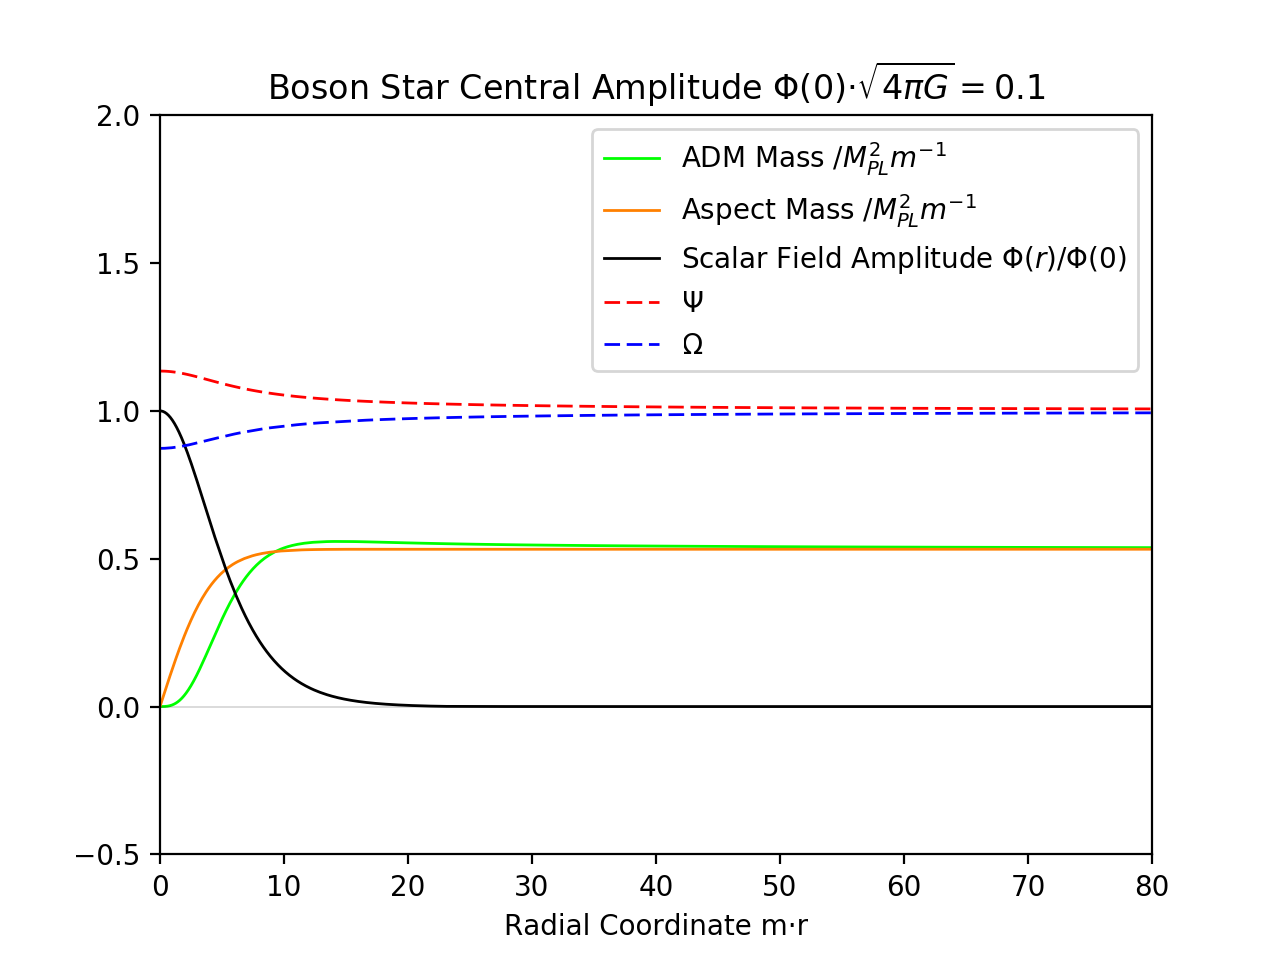
\includegraphics[width=0.5\textwidth]{png/bosonstar_groundstate.png}
%   %\hfill
%   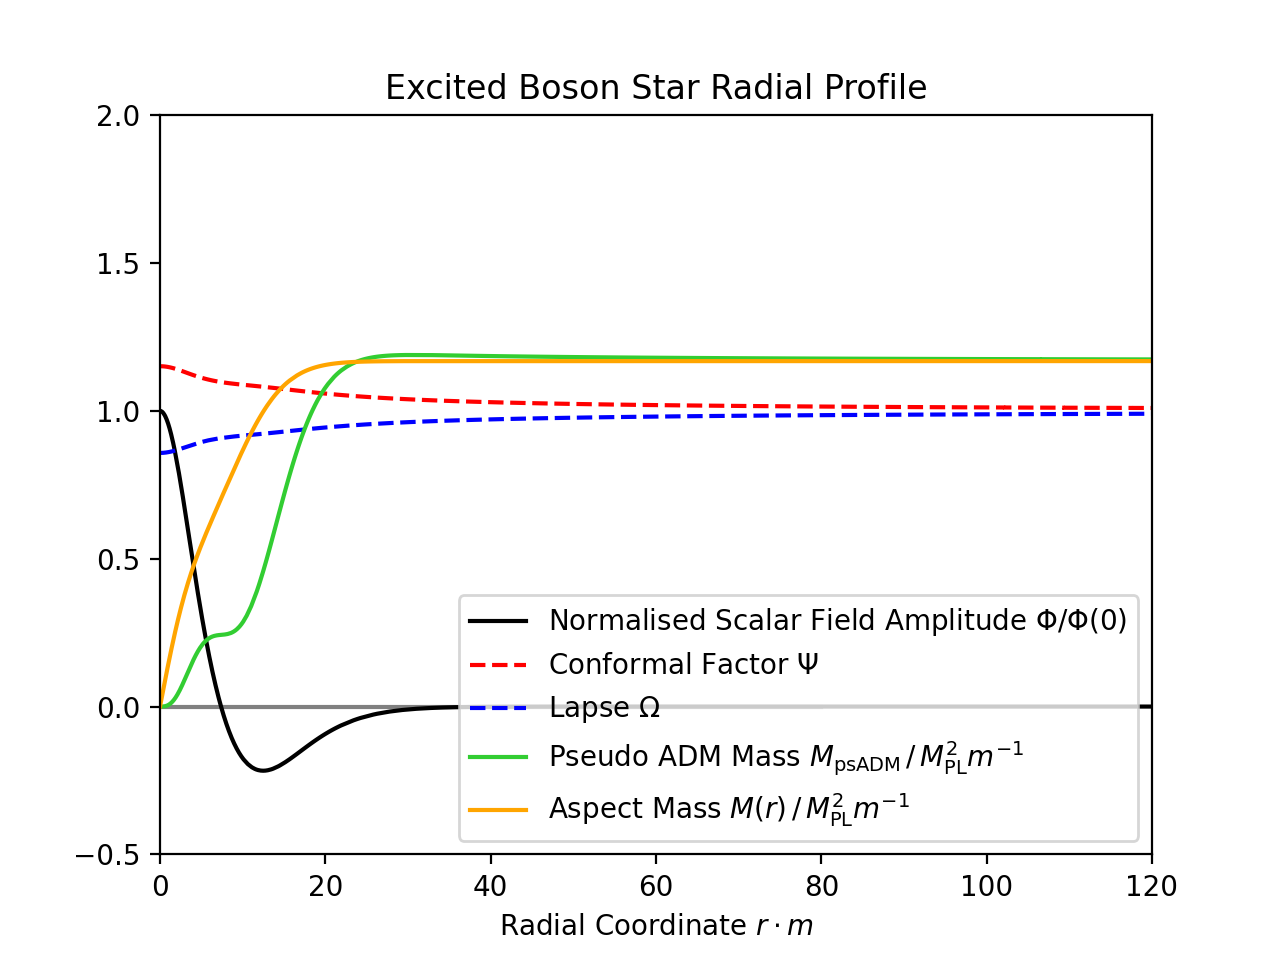
\includegraphics[width=0.5\textwidth]{png/bosonstar_excitedstate.png}
% \end{figure}

\begin{figure*}[h!]
    \subfloat%[\textsc{GRChombo}]
    {
        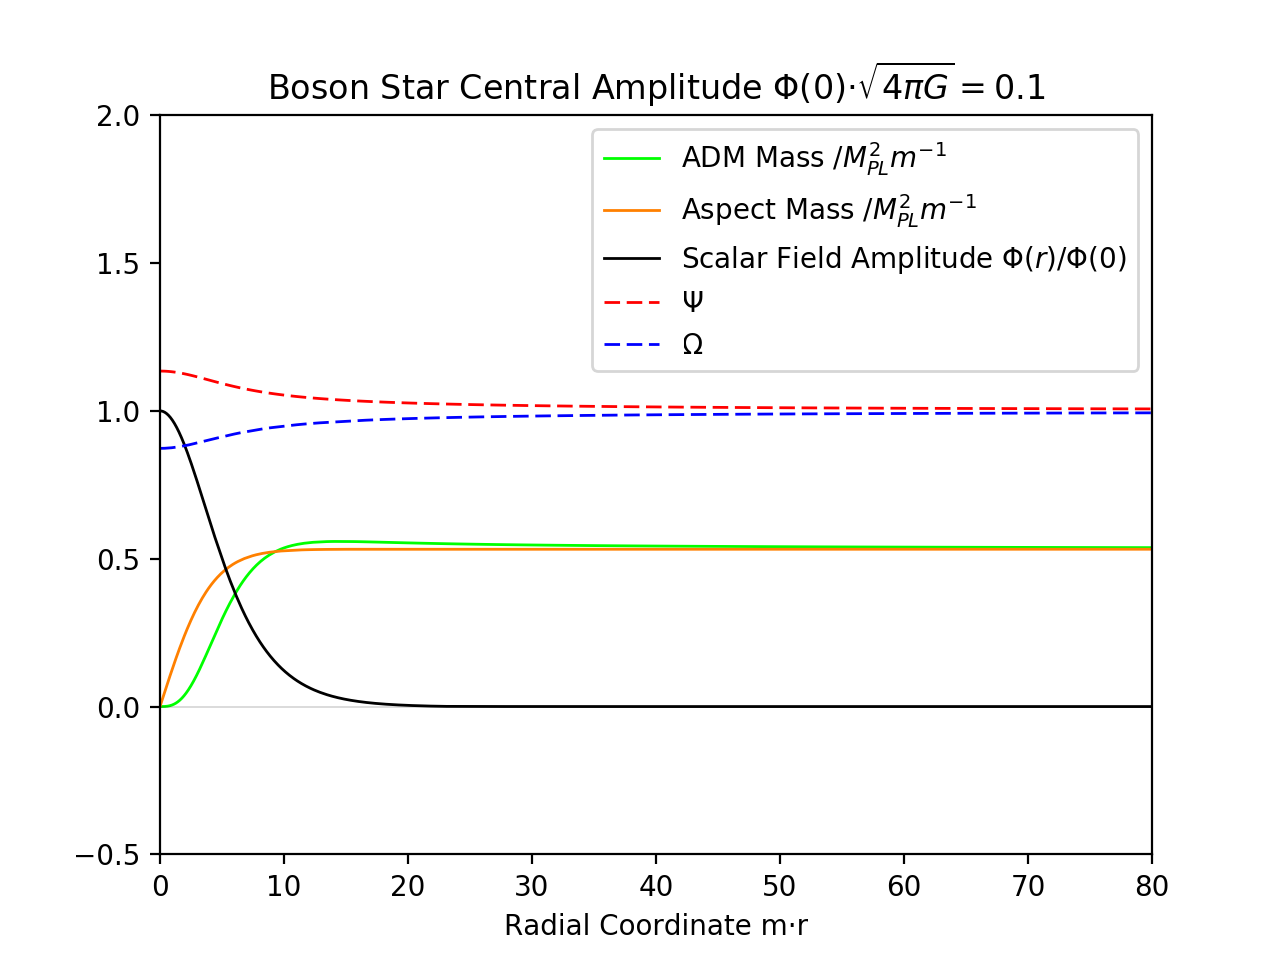
\includegraphics[width=0.48\linewidth]{png/bosonstar_groundstate.png}
        %\label{bhkick:fig:grchombo-convergence}
    }
    \hfill
    \subfloat%[\textsc{Lean}]
    {
        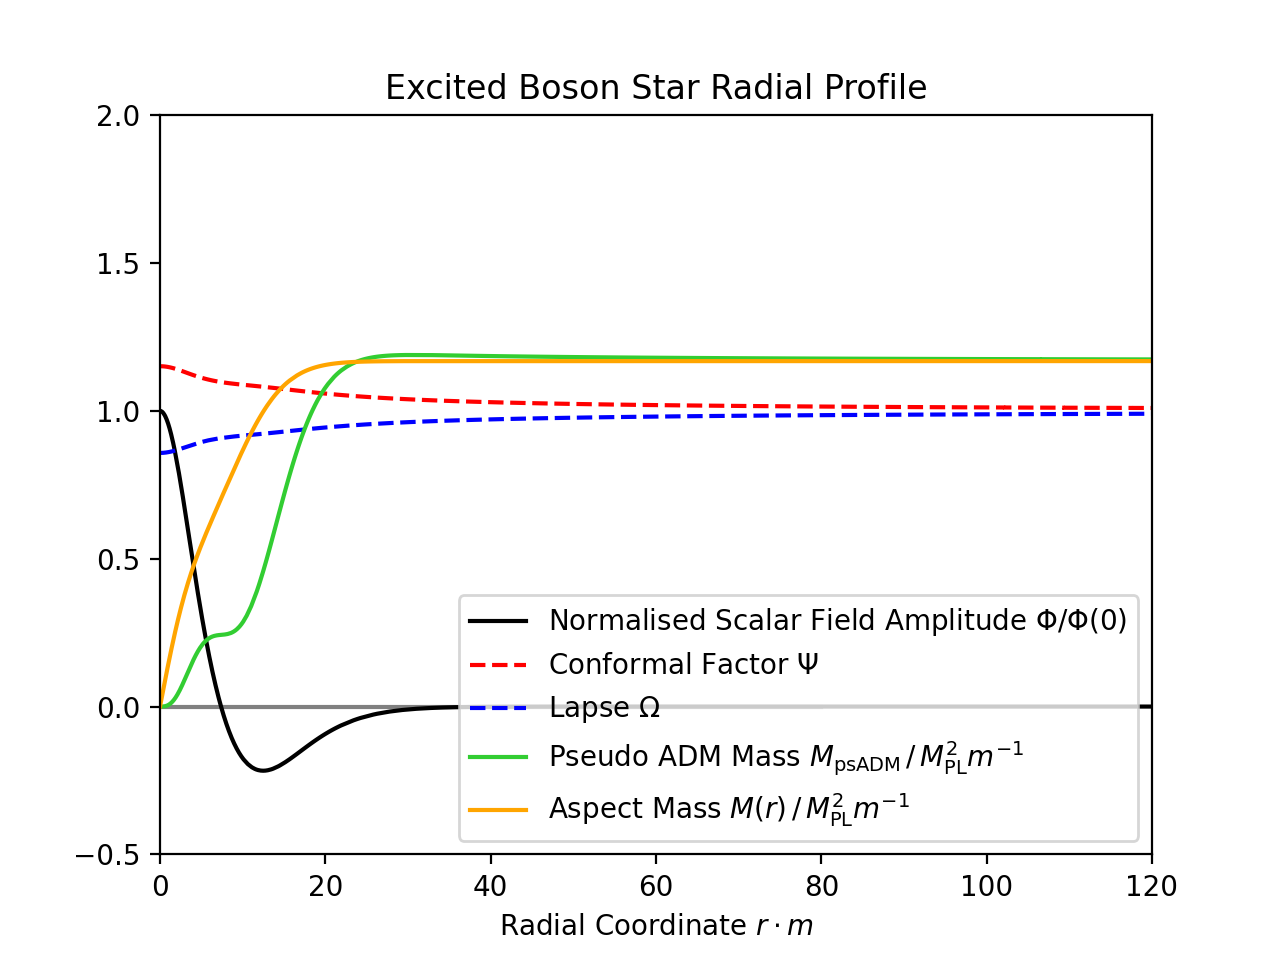
\includegraphics[width=0.48\linewidth]{png/bosonstar_excitedstate.png}
        %\label{bhkick:fig:lean-convergence}
    }
    \caption{Boson Star radial profile, Left: Ground state, Right: 1st Excited state. The ground state has an ADM mass of $M_{\rm ADM} = 0.532(5)~M_{\rm PL}^2 m^{-1}$ and the excited state has an ADM mass of $M_{\rm ADM} = 1.16(8)~M_{\rm PL}^2 m^{-1}$. Both stars have a central amplitude of $\Phi(0) \cdot \sqrt{4\pi G}=0.1 ~ m^{-1}$.
    The aspect mass is defined in Eq.~(\ref{malaise:eq:aspect_mass_def}) and the pseudo-ADM mass is given by Eq.~(\ref{boson:eq:admlike}); in the large radius limit, $M_{\rm psADM}(\infty) = M_{\rm ADM}$.}
    \label{boson:fig:f1}
\end{figure*}

%   \begin{figure}[h!]
%   \caption{Boson star radial profile for the ground state}
%   \centering
%   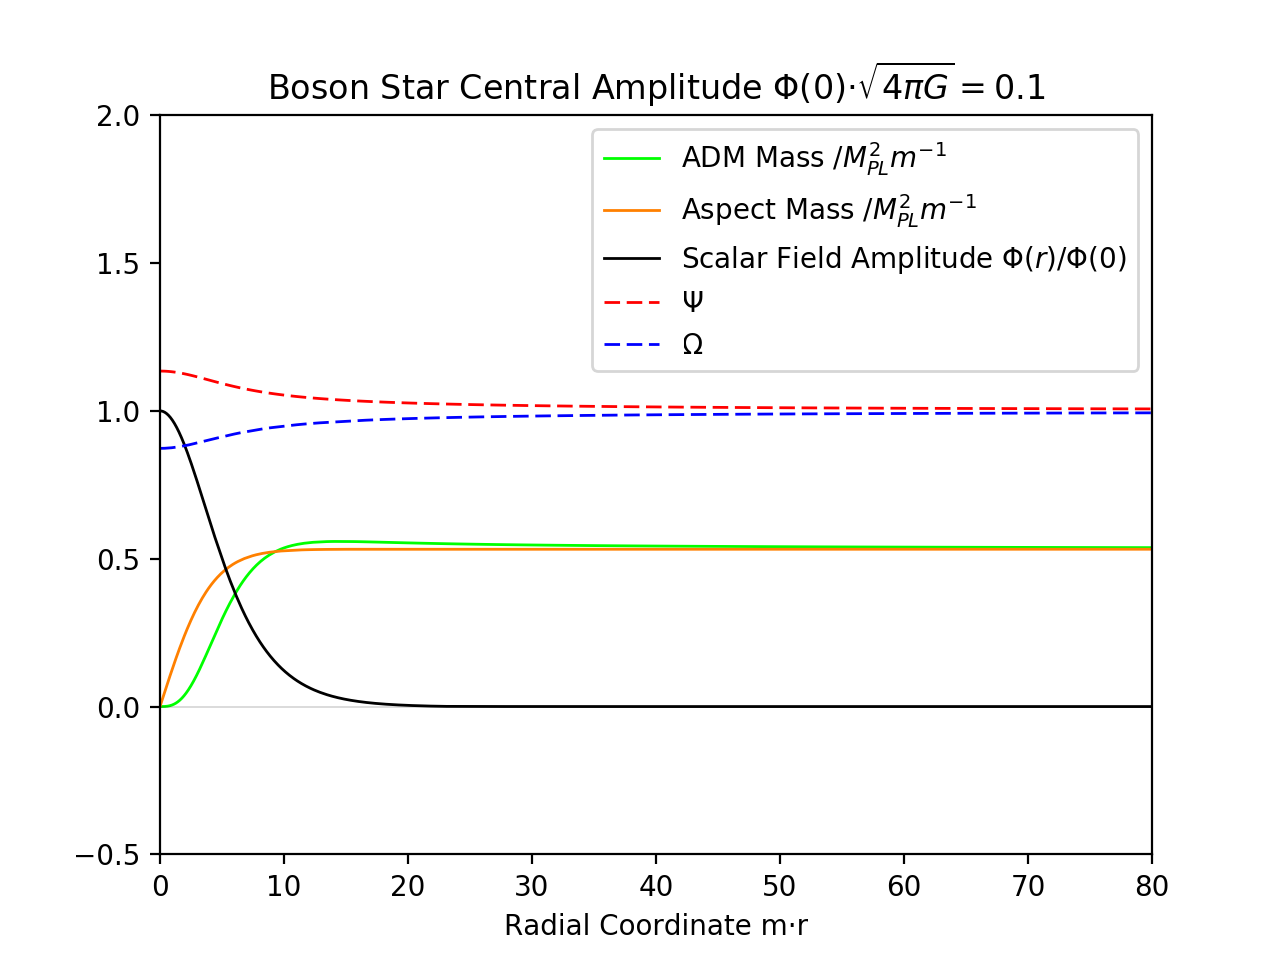
\includegraphics[width=0.8\textwidth]{png/bosonstar_groundstate.png}\label{boson:fig:f1}
% \end{figure}

%   \begin{figure}[h!]
%   \caption{Boson Star radial profile : 1st Excited state}
%   \centering
%   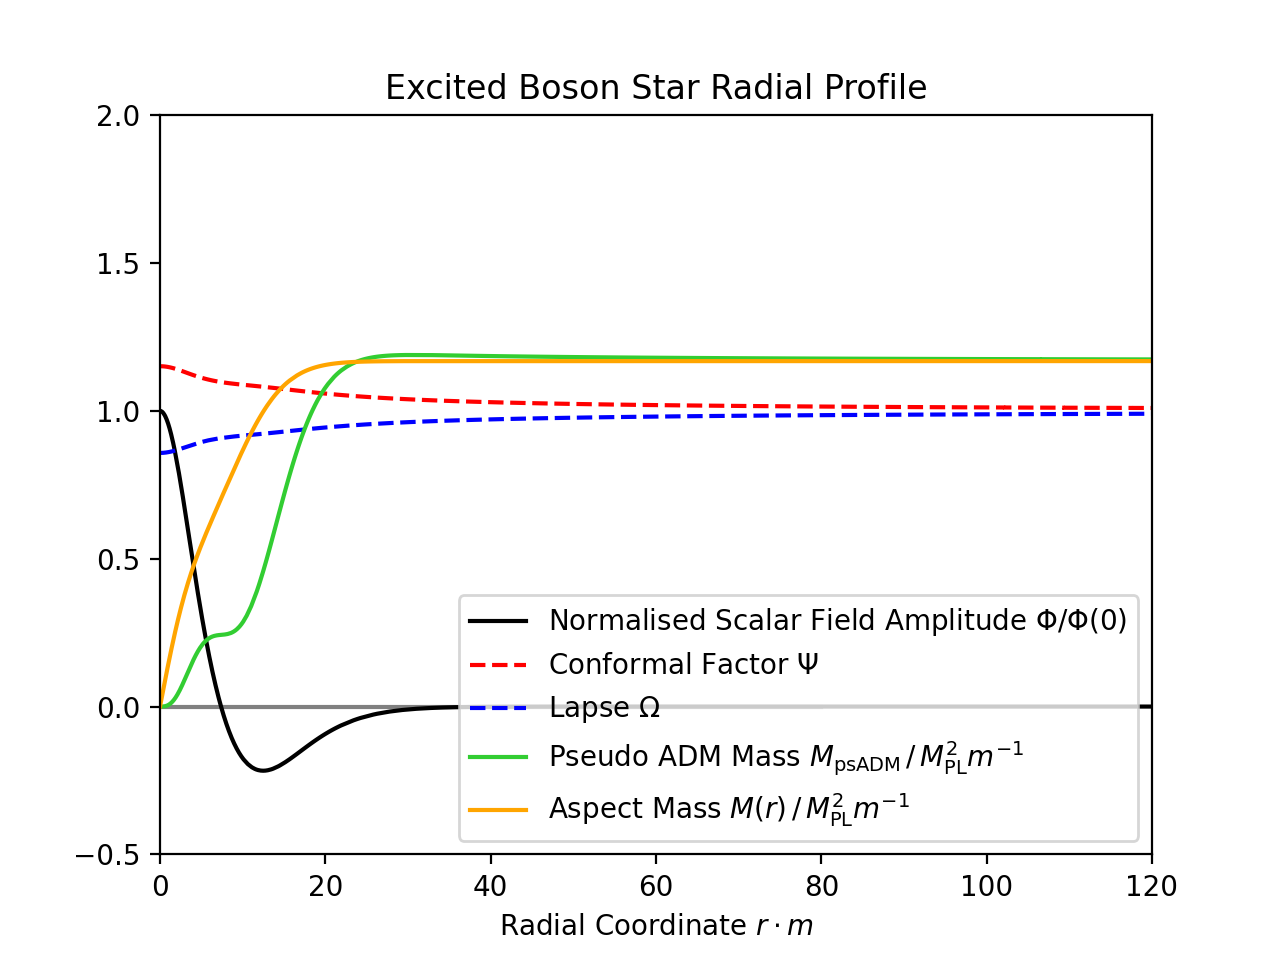
\includegraphics[width=0.8\textwidth]{png/bosonstar_excitedstate.png}\label{boson:fig:f2}
% \end{figure}


Putting everything together, a boson star solution with eigenvalue $\omega_0$
(or $\omega_n$ for excited stars) and asymptotic metric Eq.~(\ref{grchombo:eq:ABBB})
can be obtained. To find a star with asymptotic metric $\eta_{\mu\nu}$ of flat space,
the initial conditions are iteratively improved according to $\Omega_0 \rightarrow \Omega_0 /
\Omega_\infty$ and $\Psi_0 \rightarrow \Psi_0 / \Psi_\infty$; the interval bisection for
$\omega$ is then restarted. This is iterated three to five times which leaves $A=\Omega_\infty=1$
and $B=\Psi_\infty=1$ to high precision and the isotropic boson star profile has been created.
This whole process requires a few seconds runtime for a high resolution 500,000 gridpoint calculation on a regular laptop.


  \begin{figure}[h!]
  \caption{Boson star trends, Left: ADM mass vs $\Phi_0$, Right: ADM mass vs $r_{99}$}
  \centering
  \subfloat{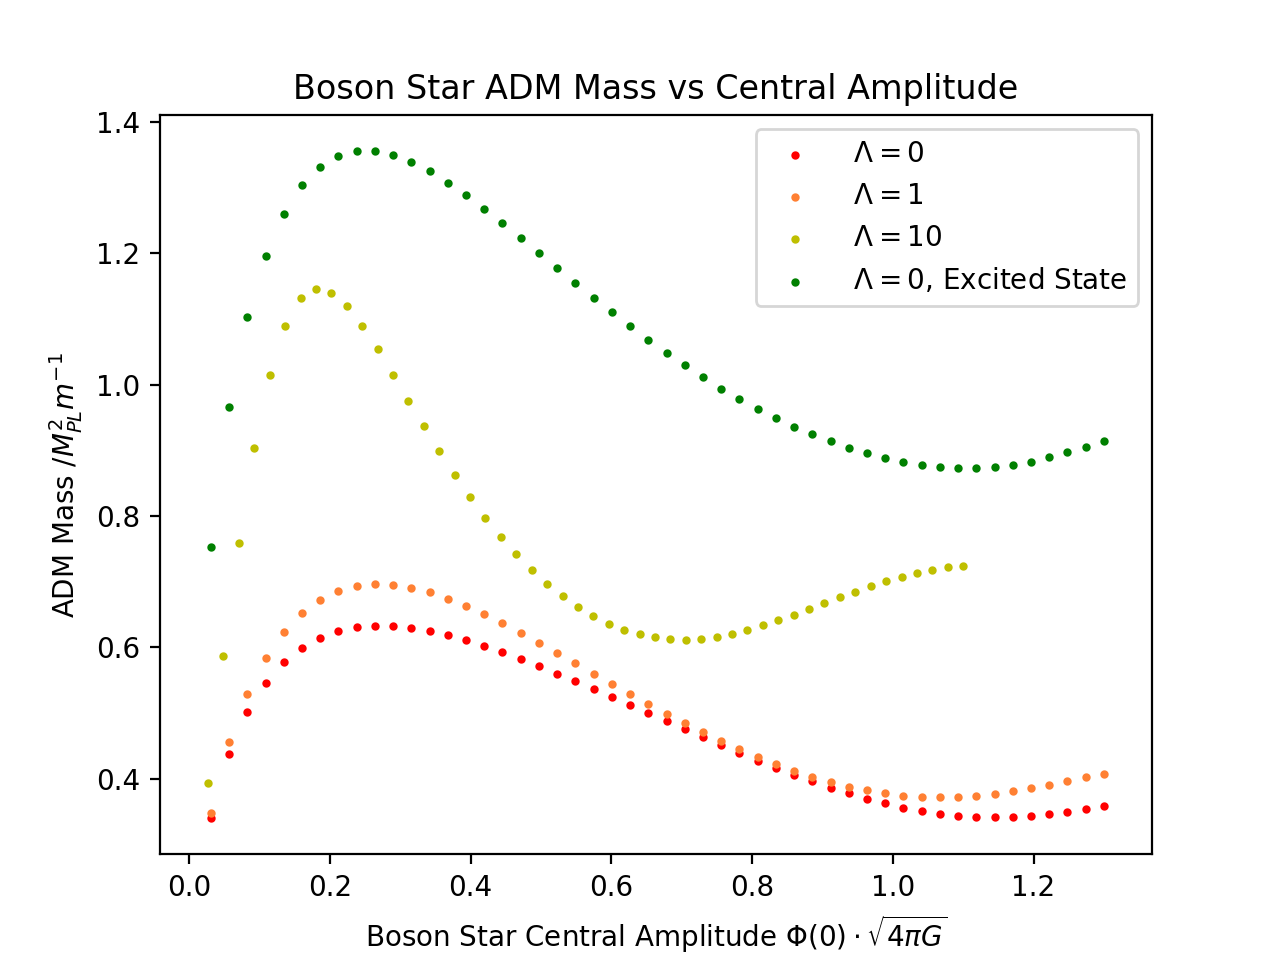
\includegraphics[width=0.48\textwidth]{png/ADM_vs_PC.png}}
  \hfill
  \subfloat{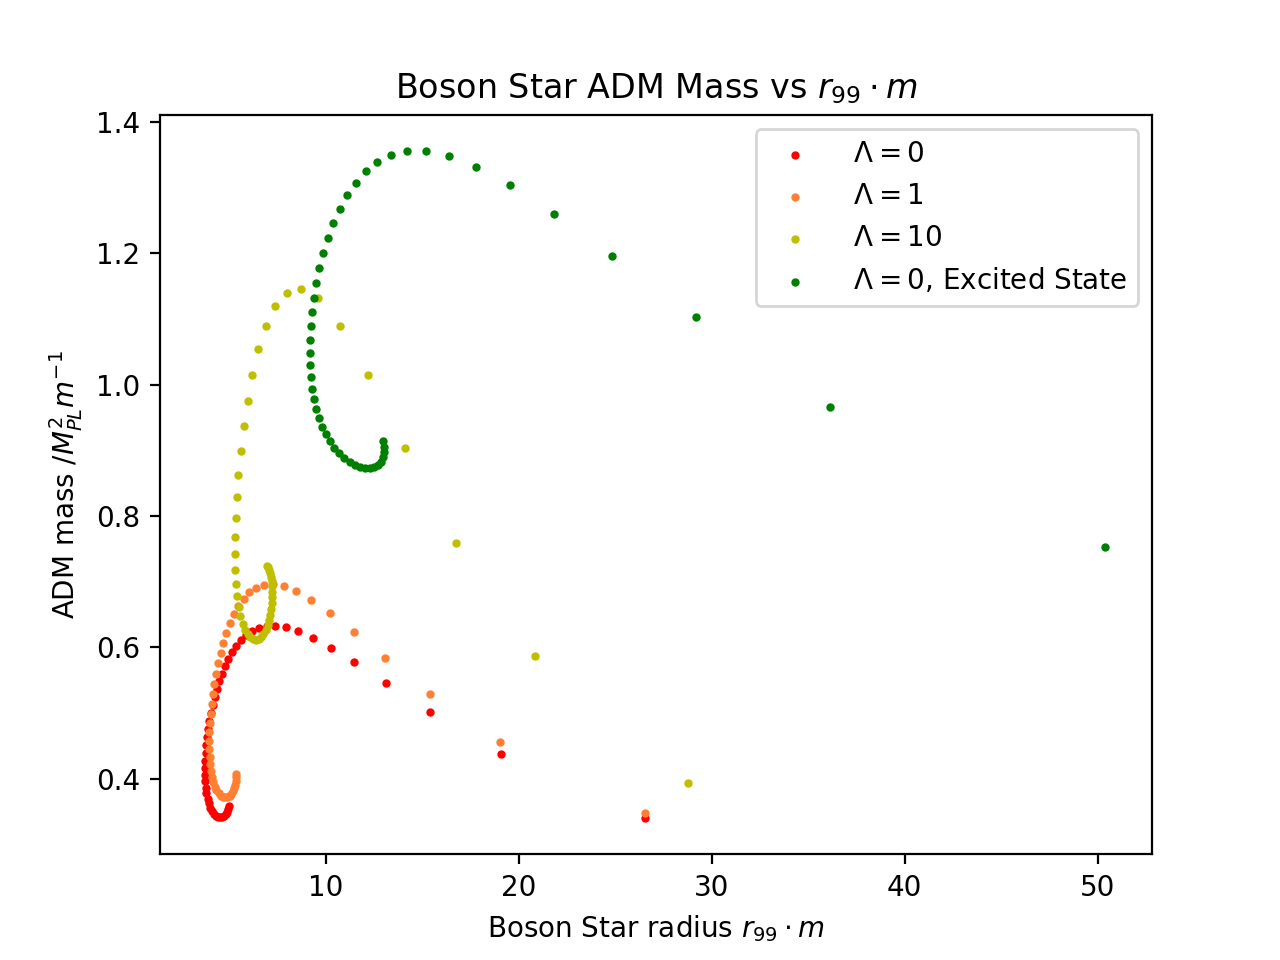
\includegraphics[width=0.48\textwidth]{png/ADM_vs_r99.png}}
  \label{boson:fig:f3}
\end{figure}

%   \begin{figure}[h!]
%   \caption{ADM mass vs $\Phi(0)$}
%   \centering
%   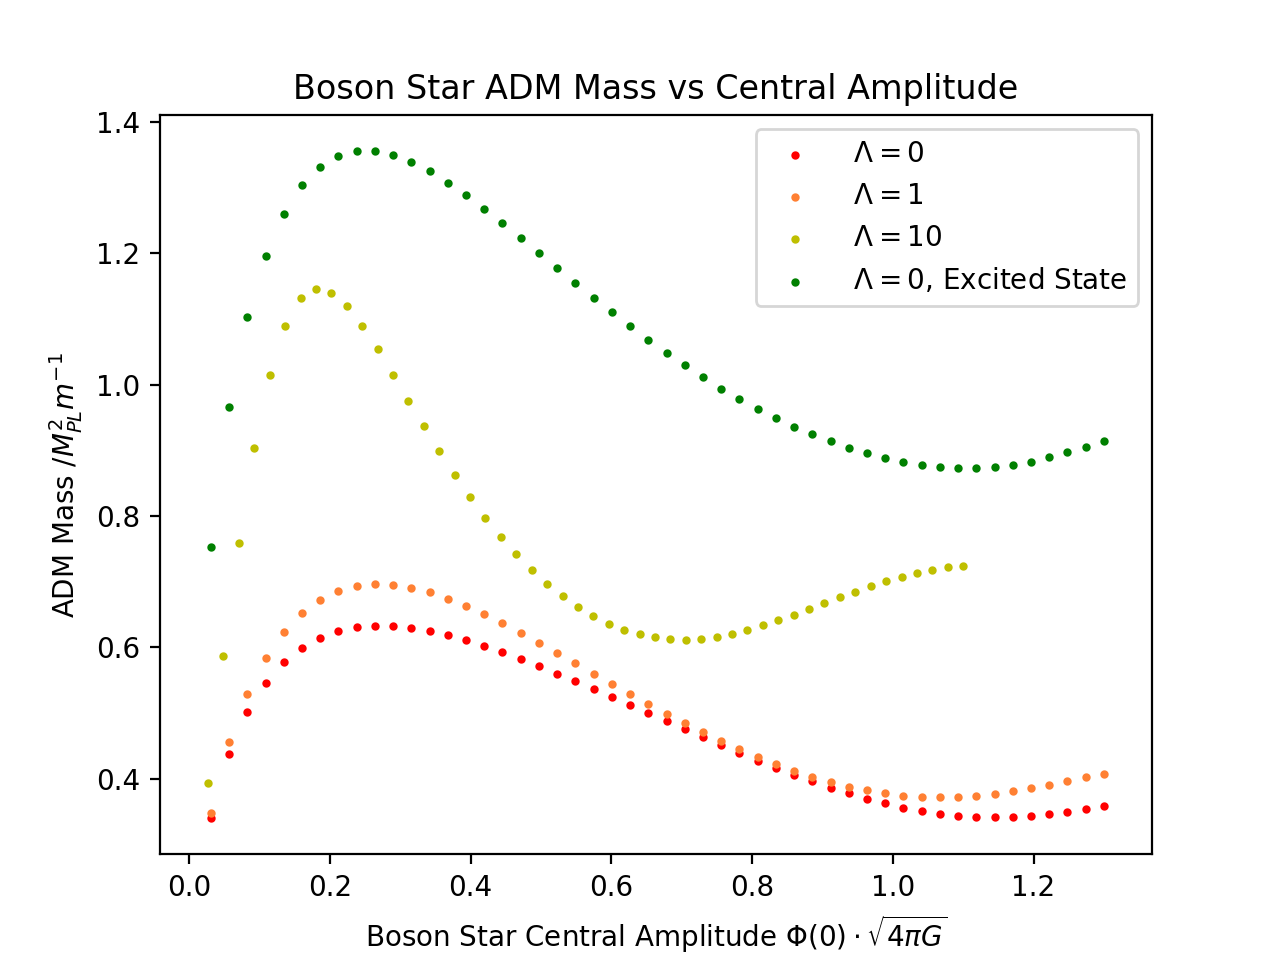
\includegraphics[width=0.8\textwidth]{png/ADM_vs_PC.png}\label{boson:fig:f1}
% \end{figure}

%   \begin{figure}[h!]
%   \caption{ADM mass vs $r_{99}$}
%   \centering
%   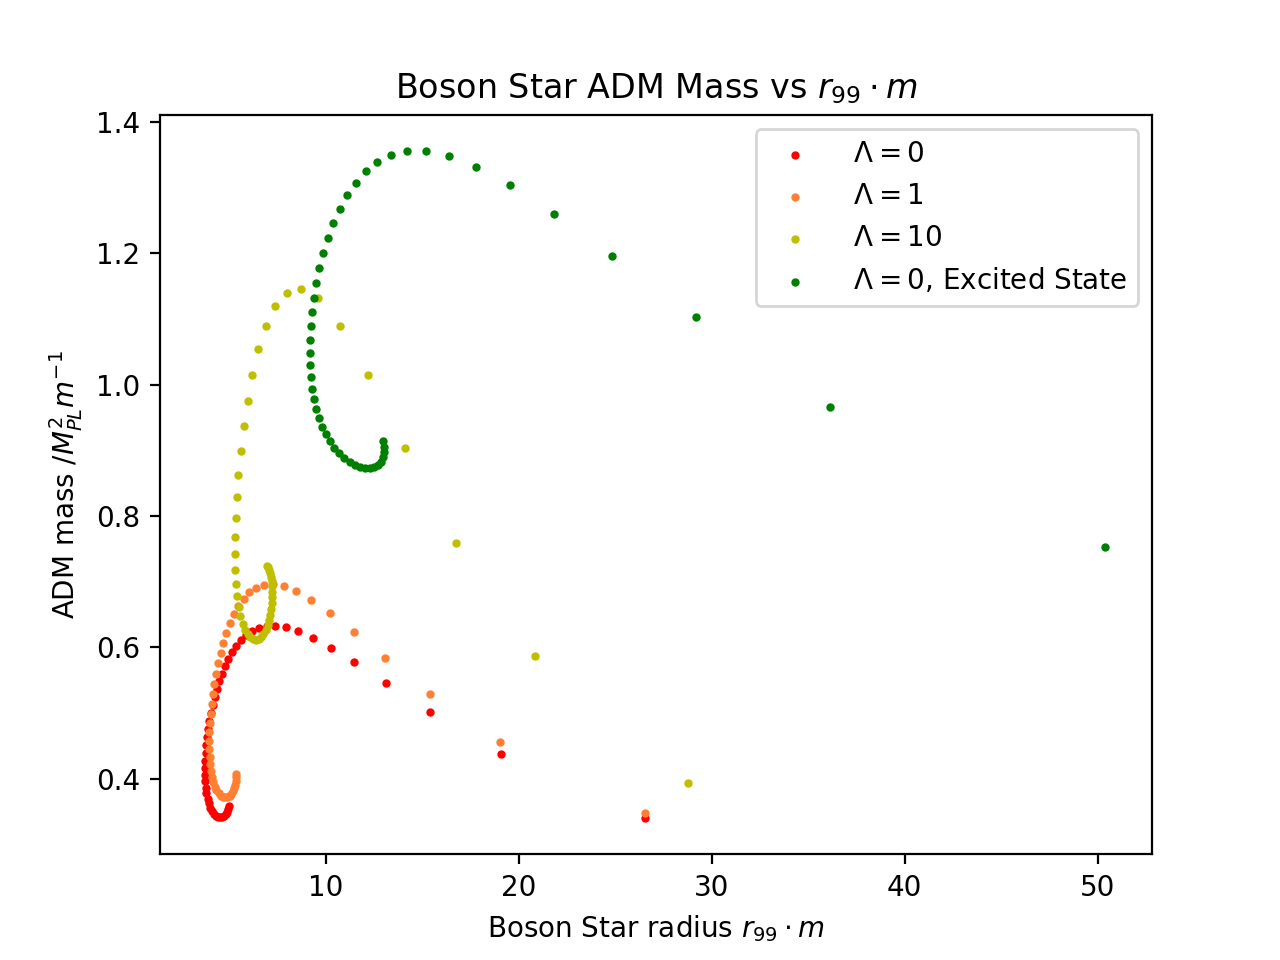
\includegraphics[width=0.8\textwidth]{png/ADM_vs_r99.png}\label{boson:fig:f2}
% \end{figure}



Figure~\ref{boson:fig:f1} shows the numerically obtained radial profile of a mini boson star ($\Lambda=0$) and an excited mini boson star. Note two mass definitions are plotted; the aspect mass defined in Eq.~(\ref{malaise:eq:aspect_mass_def}) and a pseudo-ADM mass. The conventional ADM mass \cite{arnowitt1962dynamics} is defined as
\begin{equation}
M_{\rm ADM} := \frac{1}{16\pi}\lim_{r\rightarrow\infty}\oint_{s_r} N^i \gamma^{jk}\left(\partial_j \gamma_{ik} - \partial_i \gamma_{jk} \right) \dd A,
\end{equation}
for radial coordinate $r$, 2-sphere $s_r$ of radius $r$ and unit normal vector $\bs{N}$. For an isotropic, diagonal, spherically-symmetric spatial metric ${\gamma}_{ij}$ with $\gamma_{rr} = \Psi^2(r) $, $\gamma_{\theta\theta}=\Psi^2(r)r^2$ and $\gamma_{\phi\phi}=\Psi^2(r)r^2 \sin^2\theta$ (in polar coordinates) this simplifies to,
\begin{align}
M_{\rm ADM} &= \frac{1}{16\pi}\lim_{r\rightarrow\infty}\oint_{s_r} \left(N^r \gamma^{rr}\partial_r \gamma_{rr} - N^r \gamma^{jk}\partial_r \gamma_{jk} \right) \dd A,\\
&= \frac{1}{16\pi}\lim_{r\rightarrow\infty}\oint_{s_r} N^r \Psi^{-2}\left( \partial_r \Psi^2 -  \delta^{jk}\delta_{jk}\partial_r \Psi^2 \right) \sqrt{\gamma_{\theta\theta} \gamma_{\phi\phi}} \dd \theta \dd \phi,\\
&= \frac{1}{16\pi}\lim_{r\rightarrow\infty}\int_{\theta=0}^{\theta=\pi}\int_{\phi=0}^{\phi=2\pi} -4 \Psi^{-2}\left(\partial_r \Psi \right) \Psi^2 r^2 \sin^2\theta \dd \theta \dd \phi,\\
&= \lim_{r\rightarrow\infty} \left(- r^2 \partial_r \Psi\right) ,\\
\end{align}
where we used the fact that $\bs{\gamma}(\bs{N},\bs{N})=1$ which gives $N^r = (\gamma_{rr})^{-1/2} = \Psi^{-1}$.
Note that for a Schwarzschild black hole with $\Psi = \left(1+\frac{M}{2r} \right)^2$ the ADM mass formula returns
the expected result of $M$. We define the {\it pseudo-AMD mass} as
\begin{equation}
M_{\rm psADM}(r):=- r^2 \partial_r \Psi ,\label{boson:eq:admlike}
\end{equation}
which of course satisfies $M_{\rm ADM} = M_{\rm psADM}(\infty)$.

 Polytropic fluid star initial data has also been calculated as a preliminary test
 of the code; they are easier to create as they do not require solving an eigenvalue
 problem and do not have an asymptotically growing mode. Figure~(\ref{boson:fig:f3})
 shows how the ADM mass of boson stars varies with central amplitude $\Phi_0$ and
 $r_{99}$, the radius which $\Phi(r_{99}) = \Phi_0/100$. It should be noted that
 the mini boson star (with $\Lambda =0$) case agrees with the known maximum mass,
 the Kaup limit \cite{PhysRev.172.1331} $M_{\rm max} \approx 0.633 {M_{\rm PL}^2}{m^{-1}}$
 with the largest mass being $ M_{\rm max} = 0.63299(3) {M_{\rm PL}^2}{m^{-1}} $
 corresponding to a central amplitude of $ \sqrt{4\pi G}(\Phi_0)_{\rm max} = 0.271(0)~m^{-1}$.



While many different boson stars have been computed to test the initial data code,
all the following evolutions use the same boson star with parameters $\Lambda=0$,
$\sqrt{4\pi G}\Phi_0=0.1~m^{-1} \rightarrow \Phi_0 \approx 0.0282~m^{-1}$ and
ADM mass $M=0.532(7)~M_{\rm PL}^2 m^{-1}$. This is as the stars are heavy enough
to form black holes under collisions and large deformations, but stable enough
to not collapse to a black hole for moderate perturbations.




\subsection{Single Star Evolution}

As a check that the initial data from section \ref{grchombo:sec:initialdata} is correct,
a mini boson star with central density $\Phi_0=0.02820~m^{-1}$ is evolved in time
in three spatial dimensions. The simulation has a physical domain size $L=1024~m^{-1}$
with $N=320$ gridpoints on AMR level zero with grid spacing $\Delta x = 3.2~m^{-1}$.
The AMR is allowed up to six extra levels; the finest level (level six) has a grid
spacing of $\Delta x = 0.05~m^{-1}$. The star is supposed to remain in the centre
of the grid and not change as it is a rest frame soliton; this is observed through
evolution with {\sc GRChombo}. Figure (\ref{boson:fig:f5}) shows the global maximum
value of $|\vp|$ (left figure) and the total integral of the Noether charge ${N}$
over the grid (right figure). As can be seen, $|\vp|_{\rm max}$ is constant to
$\sim 0.7\%$ and $N$ is conserved to the $\sim 0.07\%$ level until time $t=320~m^{-1}$.

  \begin{figure}[h!]
  \caption{Left: Maximum of $|\vp|$ during the evolution, Right: Total integrated Noether charge $N$.
  The initial noise seen in the two figures is attributed to junk radiation from
  refinement boundaries and is potentially exacerbated by the gauge settling from
  the initial gauge to the moving puncture gauge used. The lower-amplitude oscillation
  seen continuously in the left figure is due to finite resolution when calculating
  the maximum value $\varphi_{\rm max} = [{\rm Re}(\varphi)^2 + {\Im}(\varphi)^2]_{\rm max}$
  on any gridpoint. }
  \centering
  \subfloat{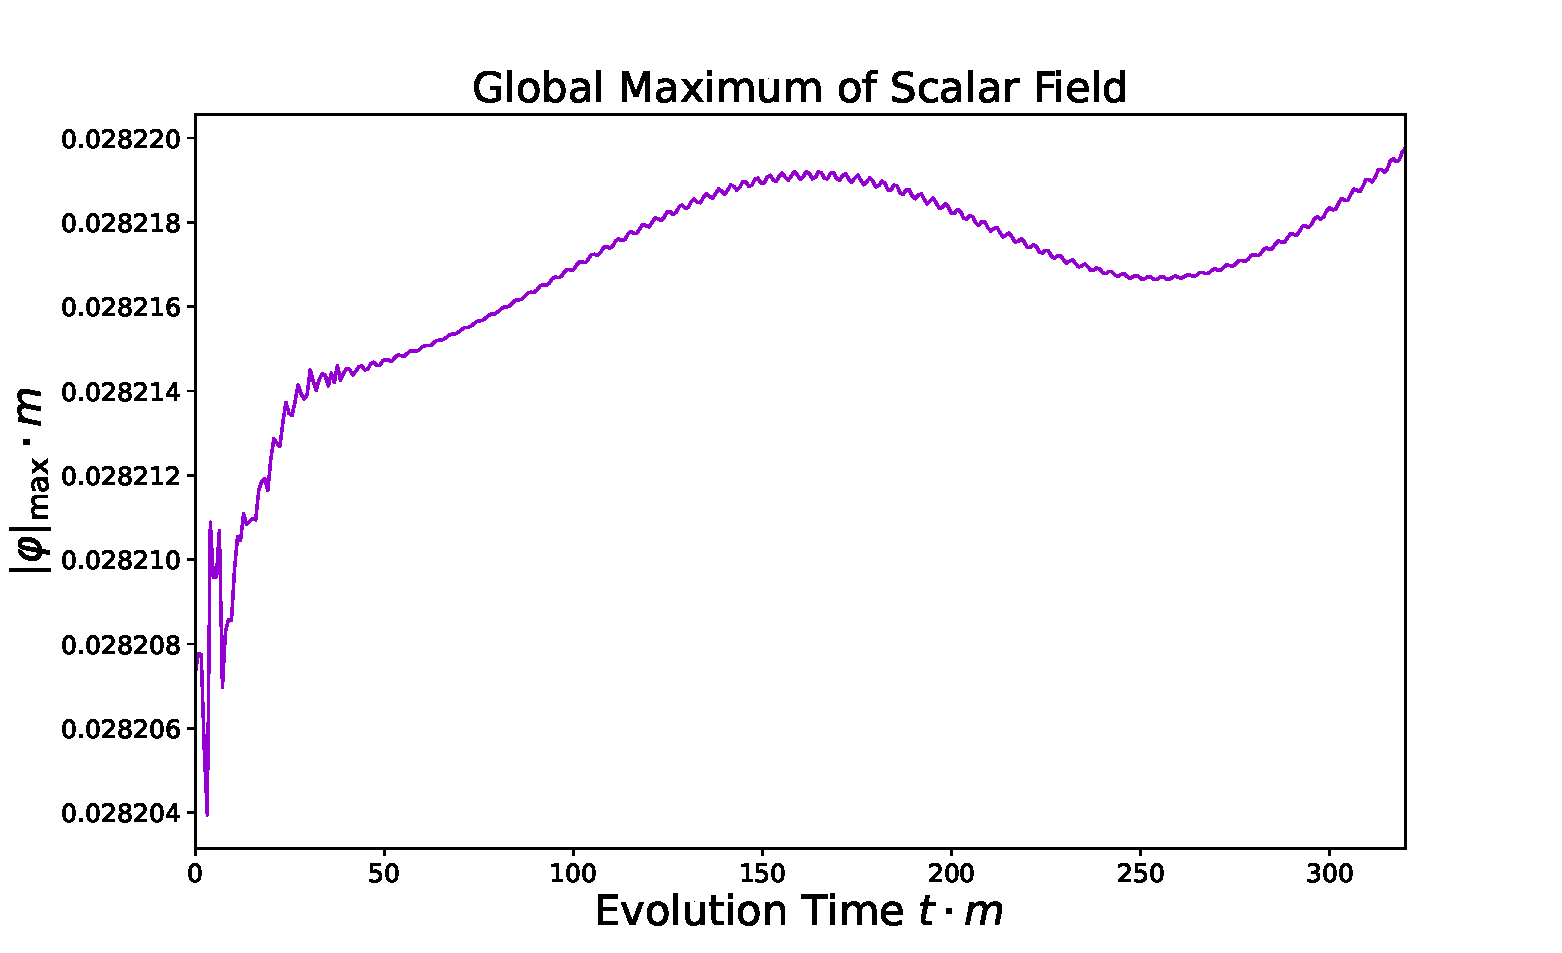
\includegraphics[width=0.5\textwidth]{data/star_modphi_nicer.pdf}}
  \hfill
  \subfloat{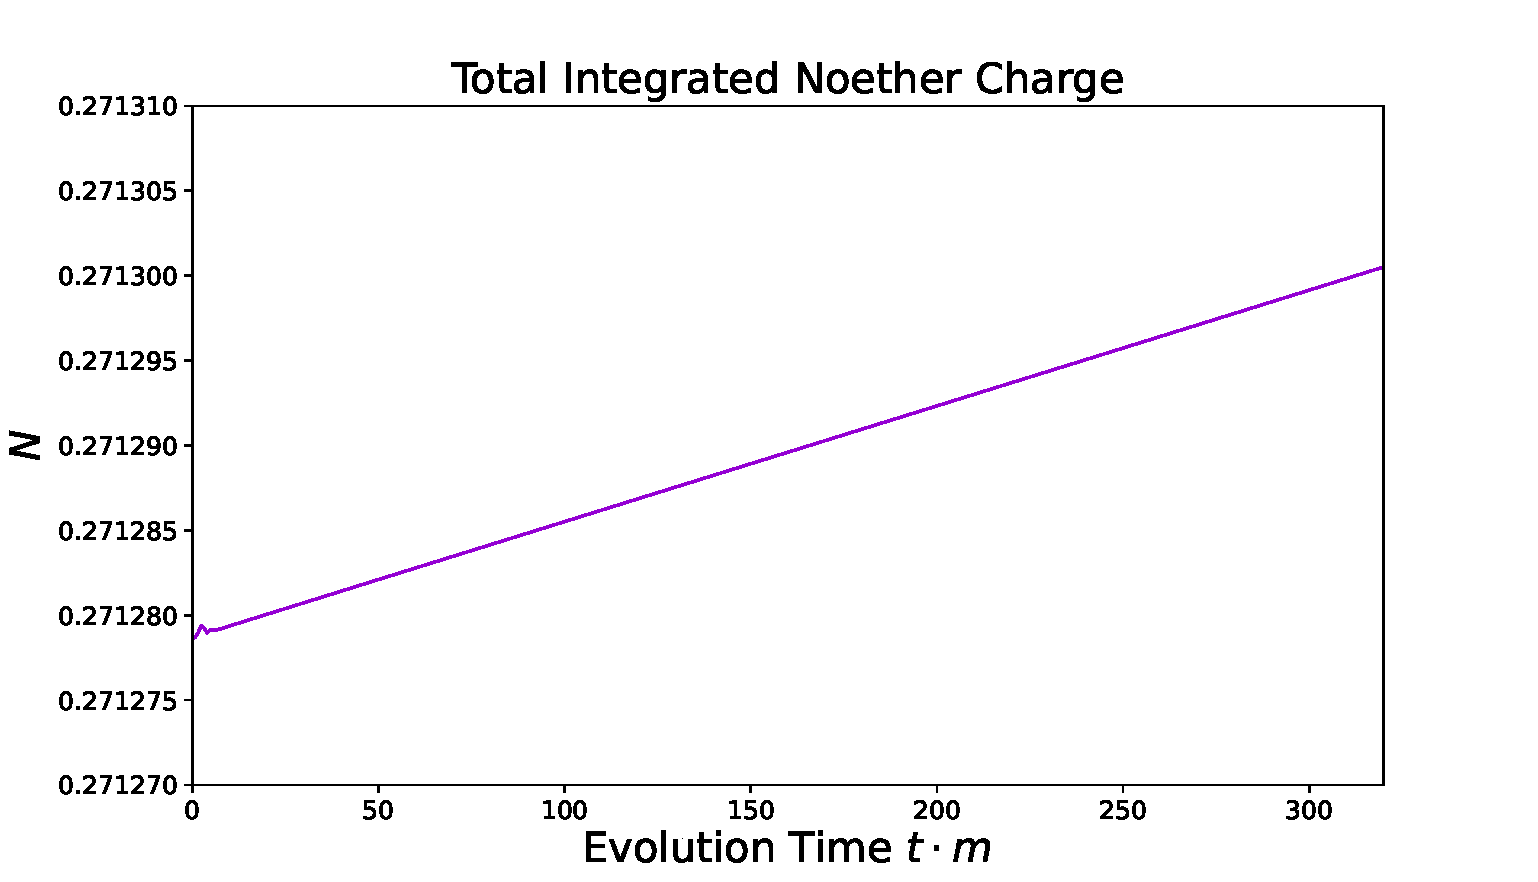
\includegraphics[width=0.5\textwidth]{data/star_N_nicer.pdf}}
  \label{boson:fig:f5}
\end{figure}






\subsection{Superposition of Initial Data} \label{grchombo:sec:superposition}
In order to simulate a spacetime consisting of two stars (or a star and a black hole) we must choose a way of superposing the initial data of two objects, centred at $x^{(1)}$ and $x^{(2)}$. For some field $\psi^{(j)}$ associated with the compact object at $x^{(j)}$,
\begin{equation}
\psi^{(j)} = \psi(x-x^{(j)}),
\end{equation} where $\psi$ refers to the object centred about the origin.
Taking two compact objects with fields $\vp$, $\Pi$, $\gamma_{ij}$, $\K_{ij}$, $\alpha$ and $\beta^i$, a naive superposition scheme was chosen;
\begin{align}
 \vp &= \vp^{(1)} + \vp^{(2)},\\
\Pi &= \Pi^{(1)} + \Pi^{(2)},\\
 \K^i_j &= {\K^{(1)}}^i_j+{\K^{(2)}}^i_j,\\
 \gamma_{\mu\nu} &= \gamma^{(1)}_{\mu\nu} + \gamma^{(2)}_{\mu\nu}-\delta_{\mu\nu},\\
\beta_i &= \beta^{(1)}_i + \beta^{(2)}_i ,\\
 \alpha &= \sqrt{\alpha_{(1)}^2 + \alpha_{(2)}^2-1},\\
 \chi &= \det\left(\gamma^{(1)}_{\mu\nu} + \gamma^{(2)}_{\mu\nu}-\delta_{\mu\nu}\right)^{-1/3},
 \end{align}
where the super-scripts ${}^{(1)}$ and ${}^{(2)}$ refer to the separate compact objects. The extrinsic curvature is chosen to be superposed with mixed indices so that it implies the trace $\mathcal{K}$ is also superposed. If one of the compact objects is a black hole the lapse $\alpha \rightarrow 0$ on the horizon; this is circumvented by setting,
\begin{equation} \alpha = \sqrt{\chi},\end{equation}
ensuring that the lapse is real and non-negative everywhere on $\Sigma_t$.

Superposing two solutions in general relativity usually no longer satisfies the Einstein equation; the Hamiltonian constraint Eq.~(\ref{nr:eq:ham}) and momentum constraints Eq.~(\ref{nr:eq:mom}) are violated. For asymptotically flat compact objects, the constraint violation reduces to zero as the object separation tends to infinity. In the case of finite separations, the CCZ4 scheme in section \ref{nr:sec:ccz4} aims to drive the constraint violation towards zero and hence a true solution of Einstein's equation; in practice, the CCZ4 scheme is more efficient at damping low amplitude, high-frequency violations and will not fully reduce long-wavelength violations \cite{gundlach2005constraint}. The collisions of compact objects in section \ref{grchombo:sec:bscollisions} use this naive superposition scheme. Section \ref{mal:sec:improvedsuperposition} explores a technique to improve the naive superposition of compact objects.



















\subsection{Collisions of Boson Stars}\label{grchombo:sec:bscollisions}



Both a headon collision and a grazing collision of two boson stars are simulated
using the superposition scheme given in section \ref{grchombo:sec:superposition}.
The two stars are identical, each has a central density of $\Phi_0=0.02820~m^{-1}$
and an ADM mass $M=0.532(7) ~M_{\rm PL}^2m^{-1}$. The stars are placed at positions
$x^i=\pm\{40,0,0\}~m^{-1}$ in the headon case and $x^i=\pm\{40,8,0\}~m^{-1}$ in
the grazing case and are boosted together with respective velocities $v^i=\mp\{0.1,0,0\}$
in both cases. A speed of $v=0.1$ corresponds to a rapidity of $\psi=0.1003353$.
The simulations have a physical domain size of $L=512~m^{-1}$ with $N=256$ gridpoints
on AMR level zero, this gives a coarse grid resolution of $\Delta x = 2~m^{-1}$.
There are up to five extra AMR levels giving a finest grid resolution of $\Delta x = 1/16~m^{-1}$.




\subsubsection{Headon Collision}
 \begin{figure}[h!]
  \caption{Left: Maximum of $|\vp|$ during evolution, Right: Total integrated Noether charge $N$.}
  \centering
  \subfloat{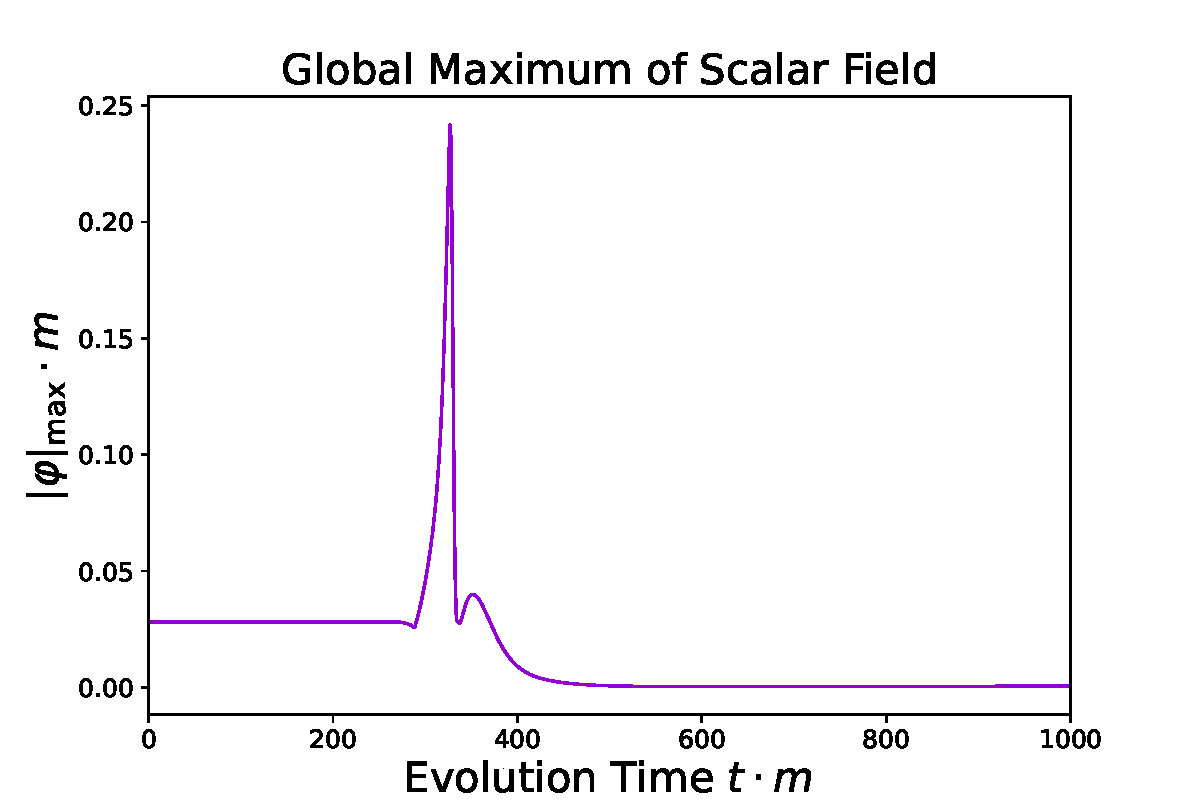
\includegraphics[width=0.5\textwidth]{data/headon_modphi_nicer.pdf}}
  \hfill
  \subfloat{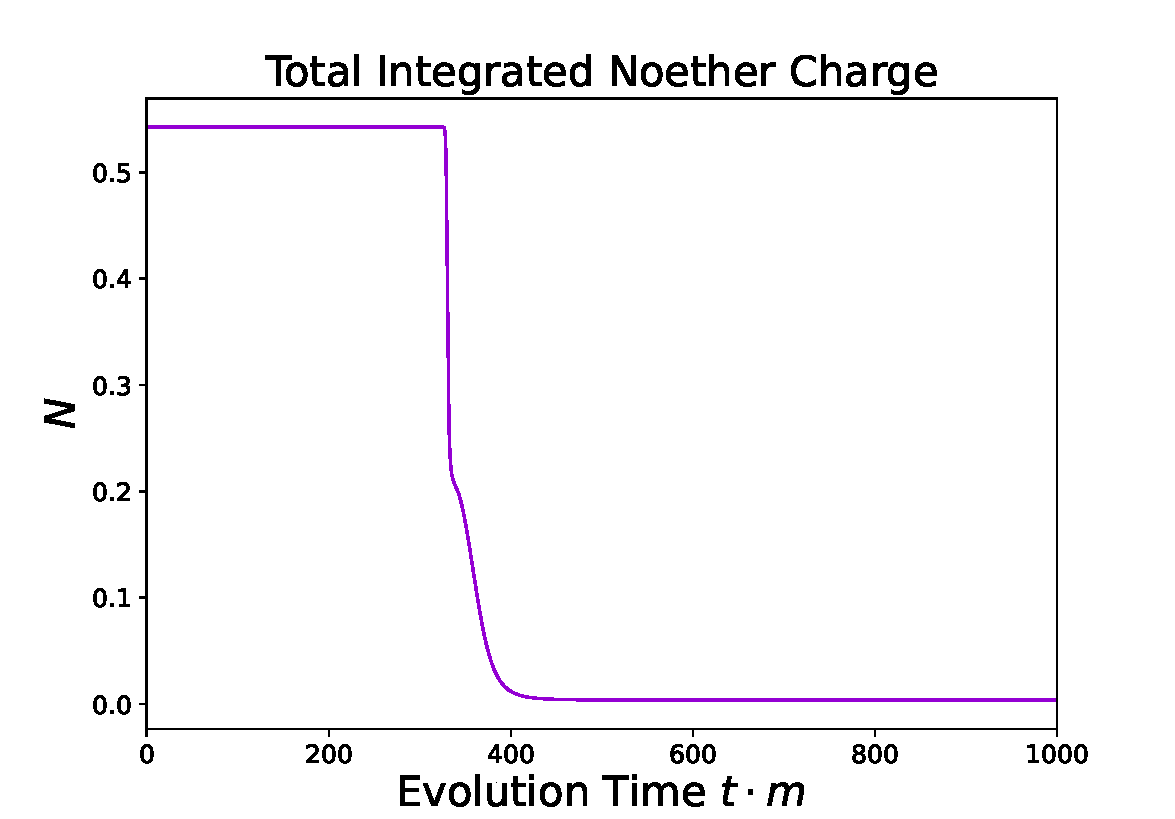
\includegraphics[width=0.5\textwidth]{data/headon_N_nicer.pdf}}
  \label{boson:fig:f7}
\end{figure}

\begin{figure}[h!]
  \caption{Gravitational wave signal of the headon boson star collision. The $l,m=2,2$ and $l,m=2,0$ spin weighted spherical harmonic modes of the $\Psi_4$ Newman-Penrose scalar are given.}
  \centering
  \subfloat{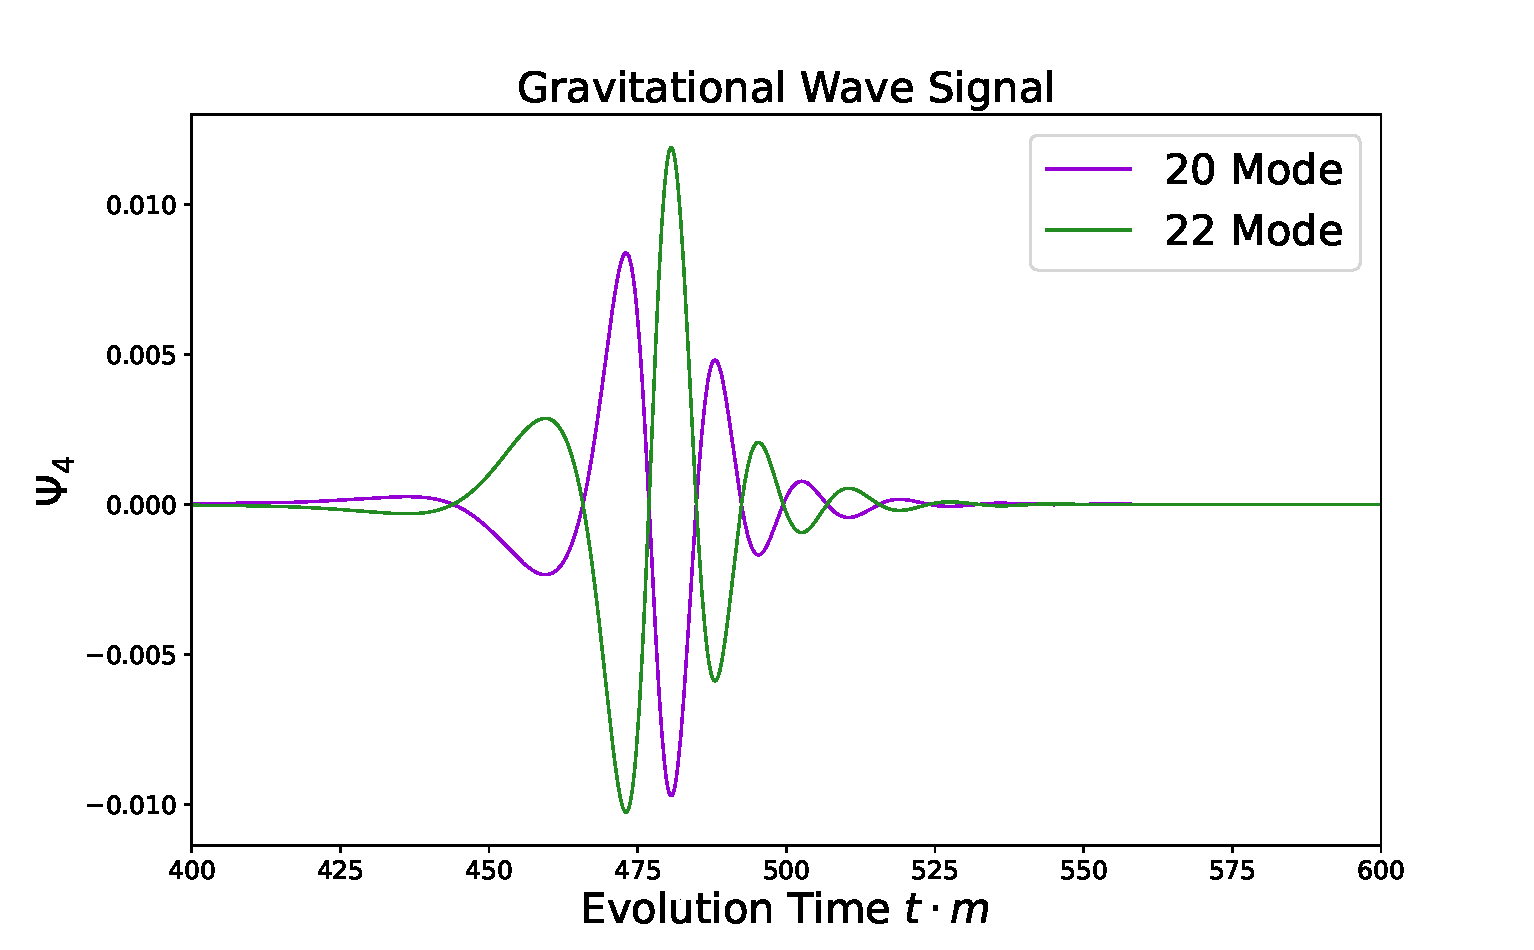
\includegraphics[width=0.5\textwidth]{data/headon_weyl_nicer.pdf}}\label{boson:fig:f9}
\end{figure}

Figure (\ref{boson:fig:f7}) shows $|\vp|_{\rm max}$, the global maximum value of $|\vp|$, and the total Noether charge $N$ as a function of time for the headon collision. At time $t\approx 289 ~m^{-1}$, $|\vp|_{\rm max}$ rapidly increases and then drops to zero, signalling the collapse to a black hole. At time $t\approx 327~m^{-1}$, there is a temporal maximum in $|\vp|_{\rm max}$ as the resolution limit of the simulation is reached and the scalar field is dissipated by the Kreiss-Oliger dissipation and diverging resolution requirements. This dissipation can also be seen in the Noether charge plot at a time of $t \approx 326~m^{-1}$ where the total charge that should remain constant but begins to fall. The lack of sufficient resolution inside the black hole is however not problematic for the external simulation; the errors accumulated are trapped inside the event horizon. Figure~(\ref{boson:fig:f7}) shows that the total Noether charge rapidly decays to zero at late time as it falls into the black hole and is dissipated.


The gravitational wave extraction at radius $r=140~m^{-1}$ is given in figure \ref{boson:fig:f9}. A spin-weighted spherical harmonic decomposition of the Newman-Penrose scalar $\Psi_4$ has been done and the $l,m = 2,0$ and $l,m = 2,2$ modes are plotted.


The dynamics of the two boson stars are shown in Fig.~(\ref{boson:fig:ff7}) which plots the scalar field modulus $|\vp|$ in the $x,y$ plane. The stars collide at time $275~m^{-1} < t < 300~m^{-1}$; which compares well to the Newtonian collision time\footnote{A simulation of point masses in Newtonian physics has been done to extract a collision time.} $t = 287.6~m^{-1}$ of two point masses with the same initial conditions. Soon after collision, an over-density of the scalar field develops which subsequently collapses to a black hole. The black hole then accretes the surrounding scalar field; the scalar field can be seen to be composed of higher order spherical harmonic modes at later times.






\subsubsection{Grazing Collision} \label{grchombo:sec:graze}

Figure (\ref{boson:fig:f10}) plots $|\vp|_{\rm max}$ and the total Noether charge
($N$) versus time for the grazing collision. At time $t\approx 309~m^{-1}$,
$|\vp|_{\rm max}$ rapidly increases and a black hole is soon formed. The black
hole is assumed\footnote{No horizon measure, or measure of angular
momentum of matter
falling into the black hole, has been done for this simulation -
these measures would be warranted in any future study.}
to be spinning due to the collapsing matter containing angular
momentum. At time $t\approx 356 ~m^{-1}$ there is a temporal maximum in $|\vp|_{\rm max}$;
similarly to the headon collision, this is caused by diverging resolution requirements
near the black hole centre and does not affect the exterior spacetime. Consequently,
the Noether charge plot shows a drop in charge at a time of $t \approx355~m^{-1}$.
 \begin{figure}[h!]
  \caption{Left: Maximum of $|\vp|$ during evolution, Right: Total integrated Noether charge $N$.}
  \centering
  \subfloat{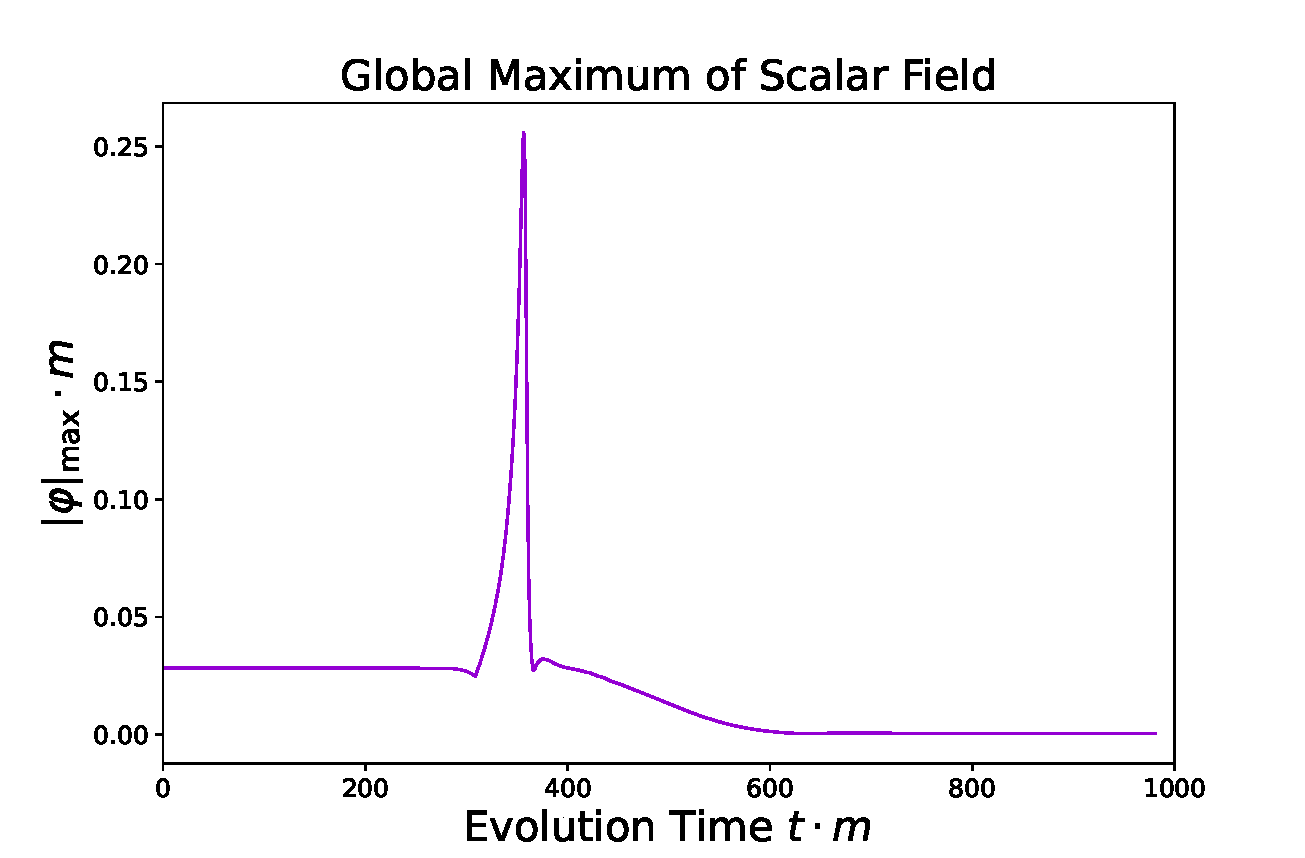
\includegraphics[width=0.5\textwidth]{data/graze_modphi_nicer.pdf}}
  \hfill
  \subfloat{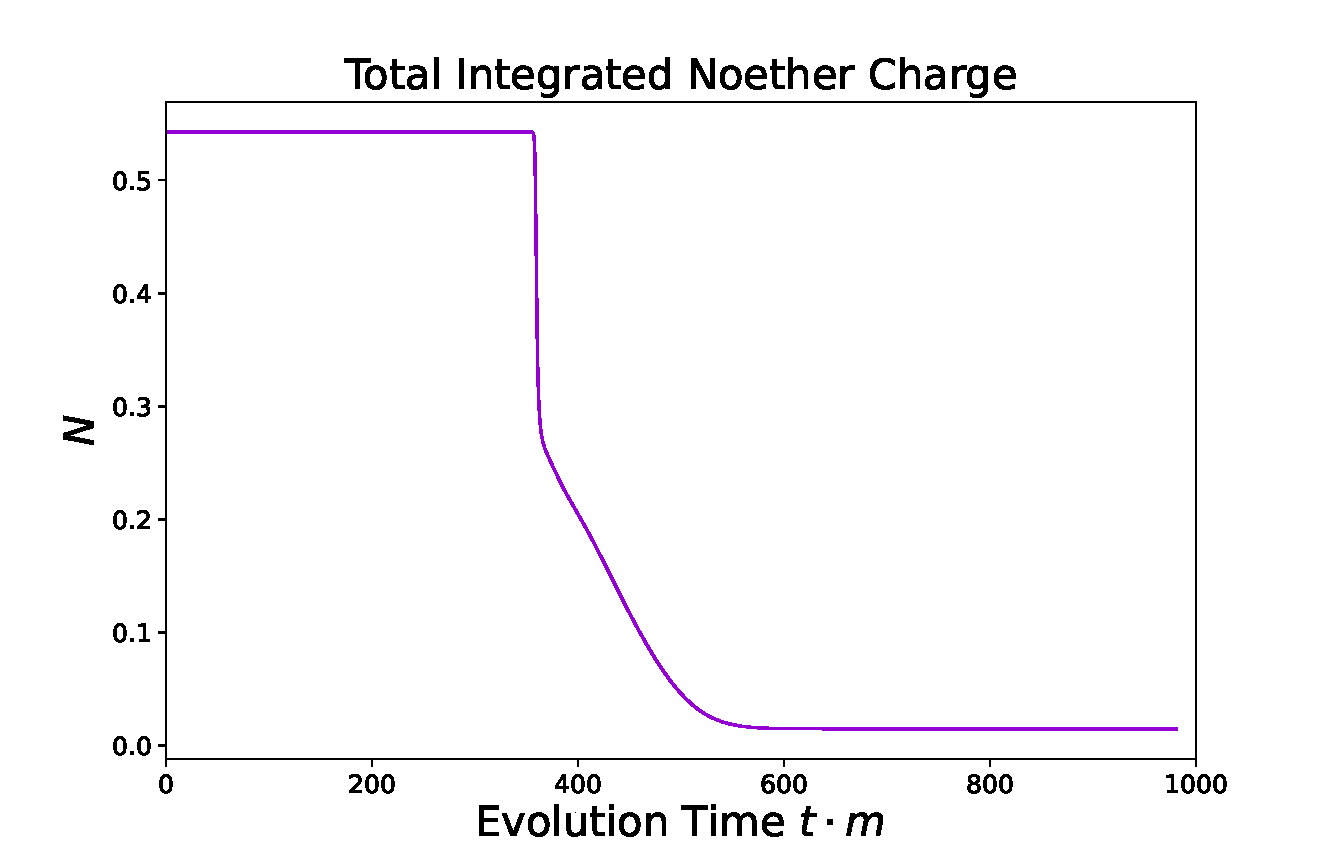
\includegraphics[width=0.5\textwidth]{data/graze_N_nicer.pdf}}
  \label{boson:fig:f10}
\end{figure}



A simulation of the grazing collision with point masses has been done using Newtons laws. The time taken for closest approach (with separation $s = 2.33~m^{-1}$) is $t=315.8~m^{-1}$; at this separation the finite sized stars would collide. Snapshots of the grazing boson star collision using numerical relativity (in full general relativity) are shown in Fig.~(\ref{boson:fig:ff10}) plotting the scalar field modulus $|\vp|$ in the $x,y$ plane. The stars collide at time $300~m^{-1} < t < ~m^{-1}$ which is in good agreement with the Newtonian approximation. Soon after collision, an over-density of the scalar field develops and collapses to a black hole; this black hole is thought to be spinning due to the angular momentum of the collapsing matter. The black hole subsequently accretes most of the surrounding scalar field leaving a quasi-long-lived rotating toroidal scalar field configuration surrounding the black hole. This late time toroidal scalar field configuration will be referred to as a {\it toroidal wig} due to it being \enquote{fake} hair. The late time toroidal wig seems to settle to a rotationally symmetric configuration, with no quadrupole moment, and does not emit a significant gravitational wave signal; this can be seen in Fig.~(\ref{boson:fig:f12}) which plots the $l,m=2,2$ and $l,m=2,0$ modes of $\Psi_4$.



\begin{figure}[h!]
  \caption{Gravitational wave signal of the grazing boson star collision. The $l,m=2,2$ and $l,m=2,0$ modes of the $\Psi_4$ Newman-Penrose scalar are given.}
  \centering
  \subfloat{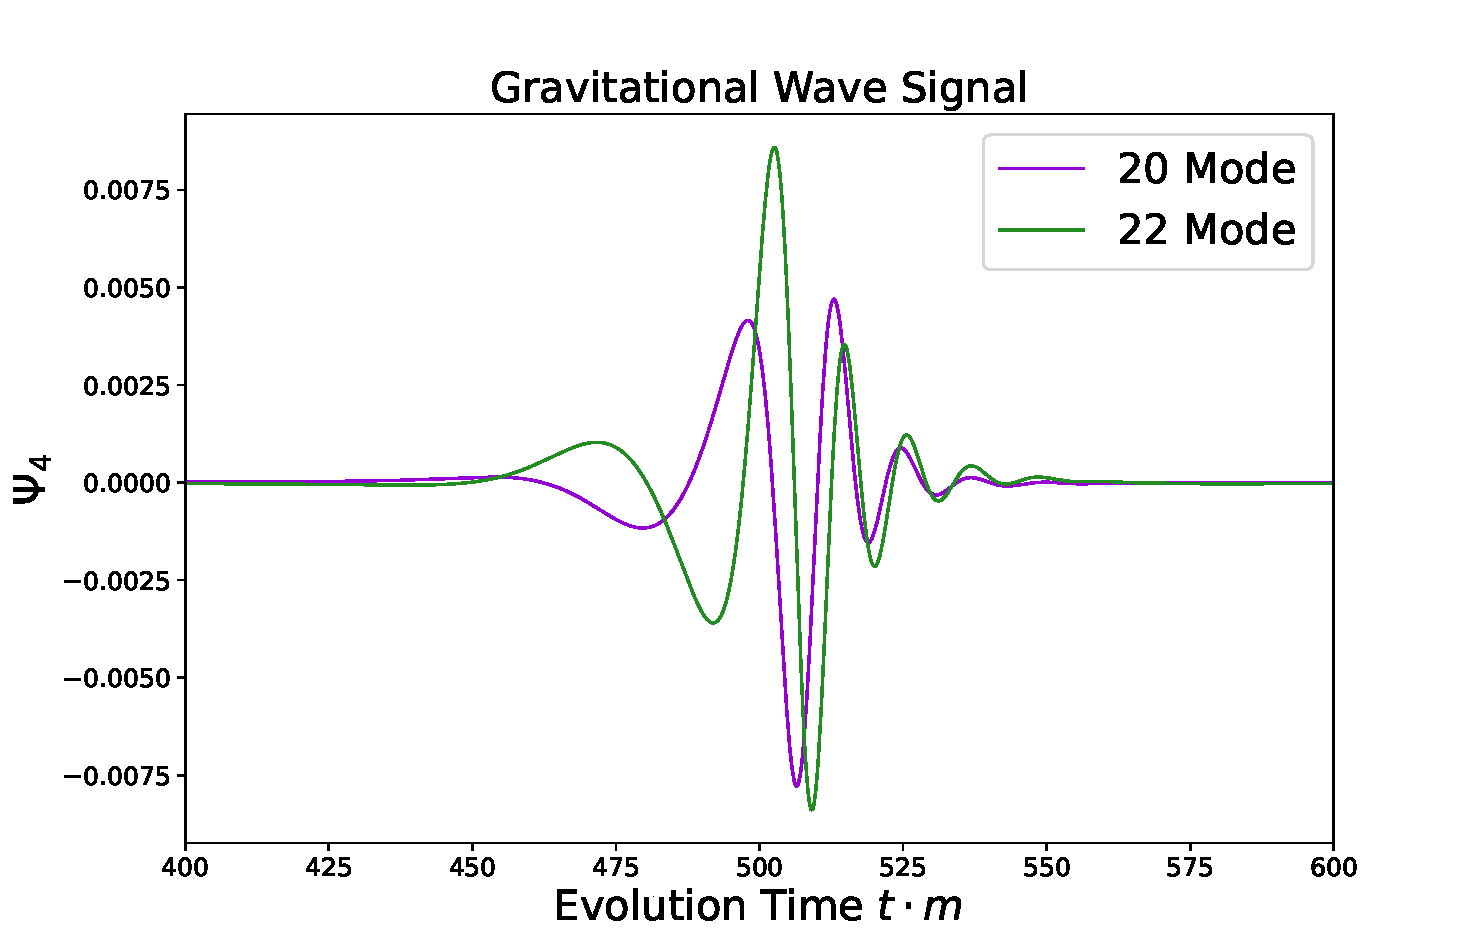
\includegraphics[width=0.5\textwidth]{data/graze_weyl_nicer.pdf}}
  \label{boson:fig:f12}
\end{figure}

 \begin{figure}[h!]
\caption{Left: Comparison of late time Noether charge $N$ between headon collision and grazing collision of two boson stars. Right: Late time plot of the Noether charge of the grazing collision only.}
\subfloat{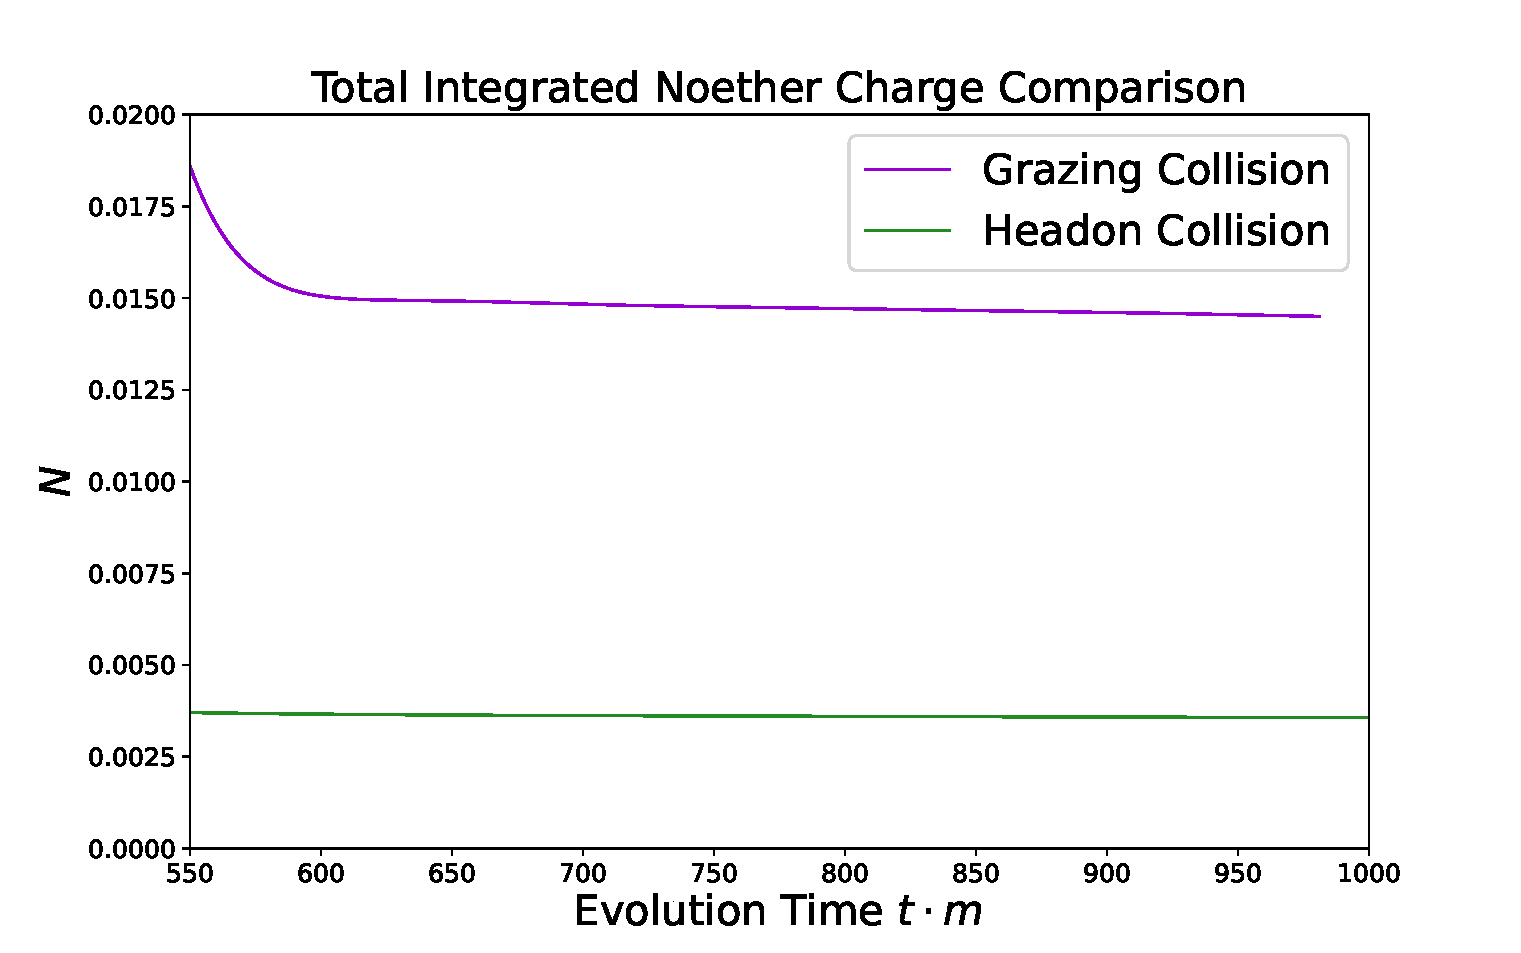
\includegraphics[width=0.45\textwidth]{data/late_time_N_nicer.pdf}}
\subfloat{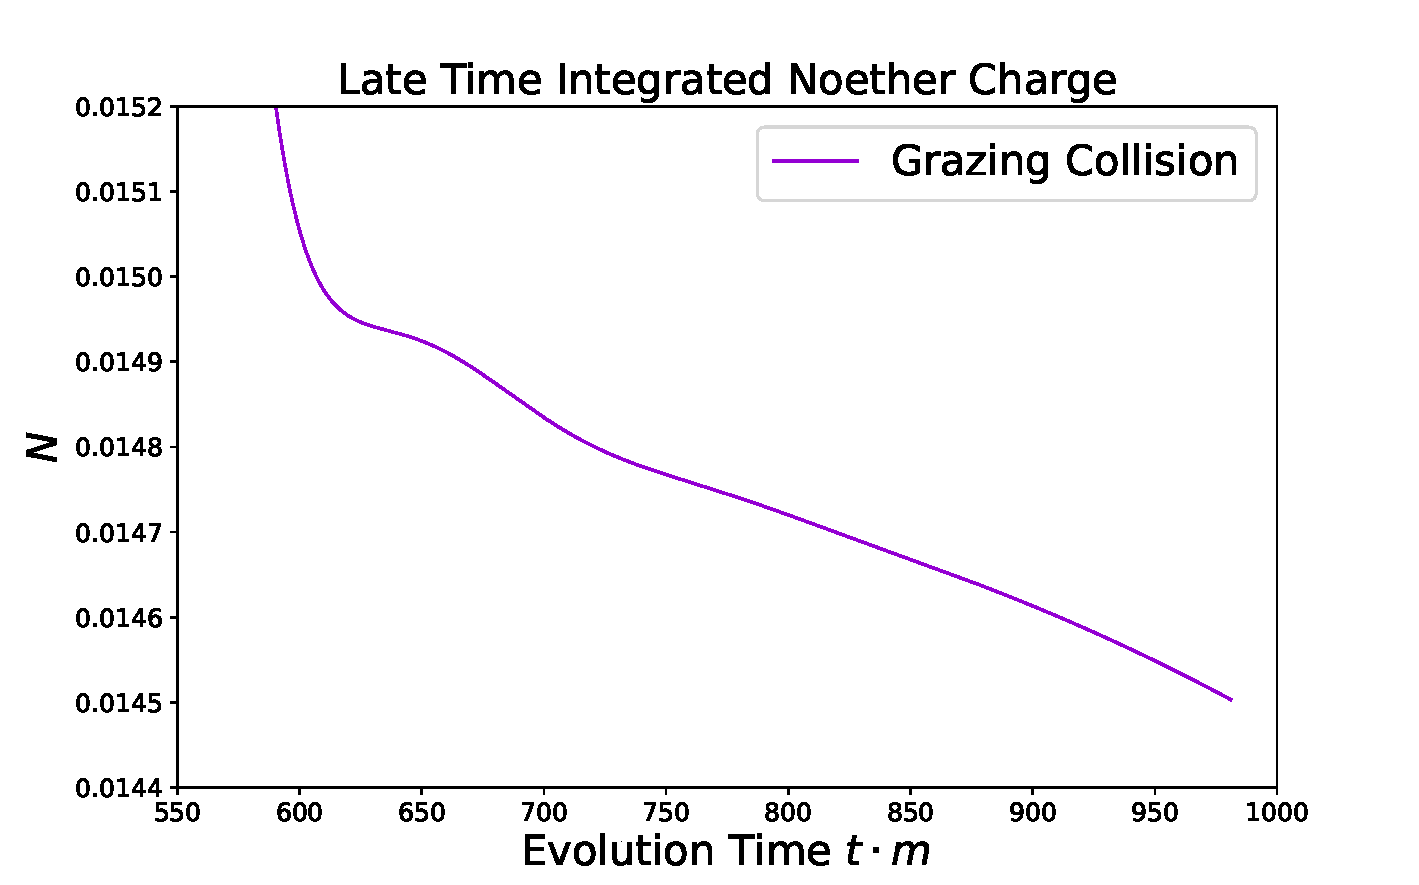
\includegraphics[width=0.45\textwidth]{data/noether_zoom_nicer.pdf}}
\label{boson:fig:fff}
\end{figure}



Figure (\ref{boson:fig:fff}) shows the late time Noether charge of the grazing and headon collisions. In contrast to the headon collision, the decay of $N$ in the grazing case is slower and reaches a value approximately $7$ times greater. Using linear extrapolation, the Noether charge of the grazing collision decays to zero at time $t \approx 12500 ~m^{-1} $ and hence the toroidal wig has an approximate lifespan of $12000~m^{-1}$.





 \begin{figure}[h!]
  \subfloat{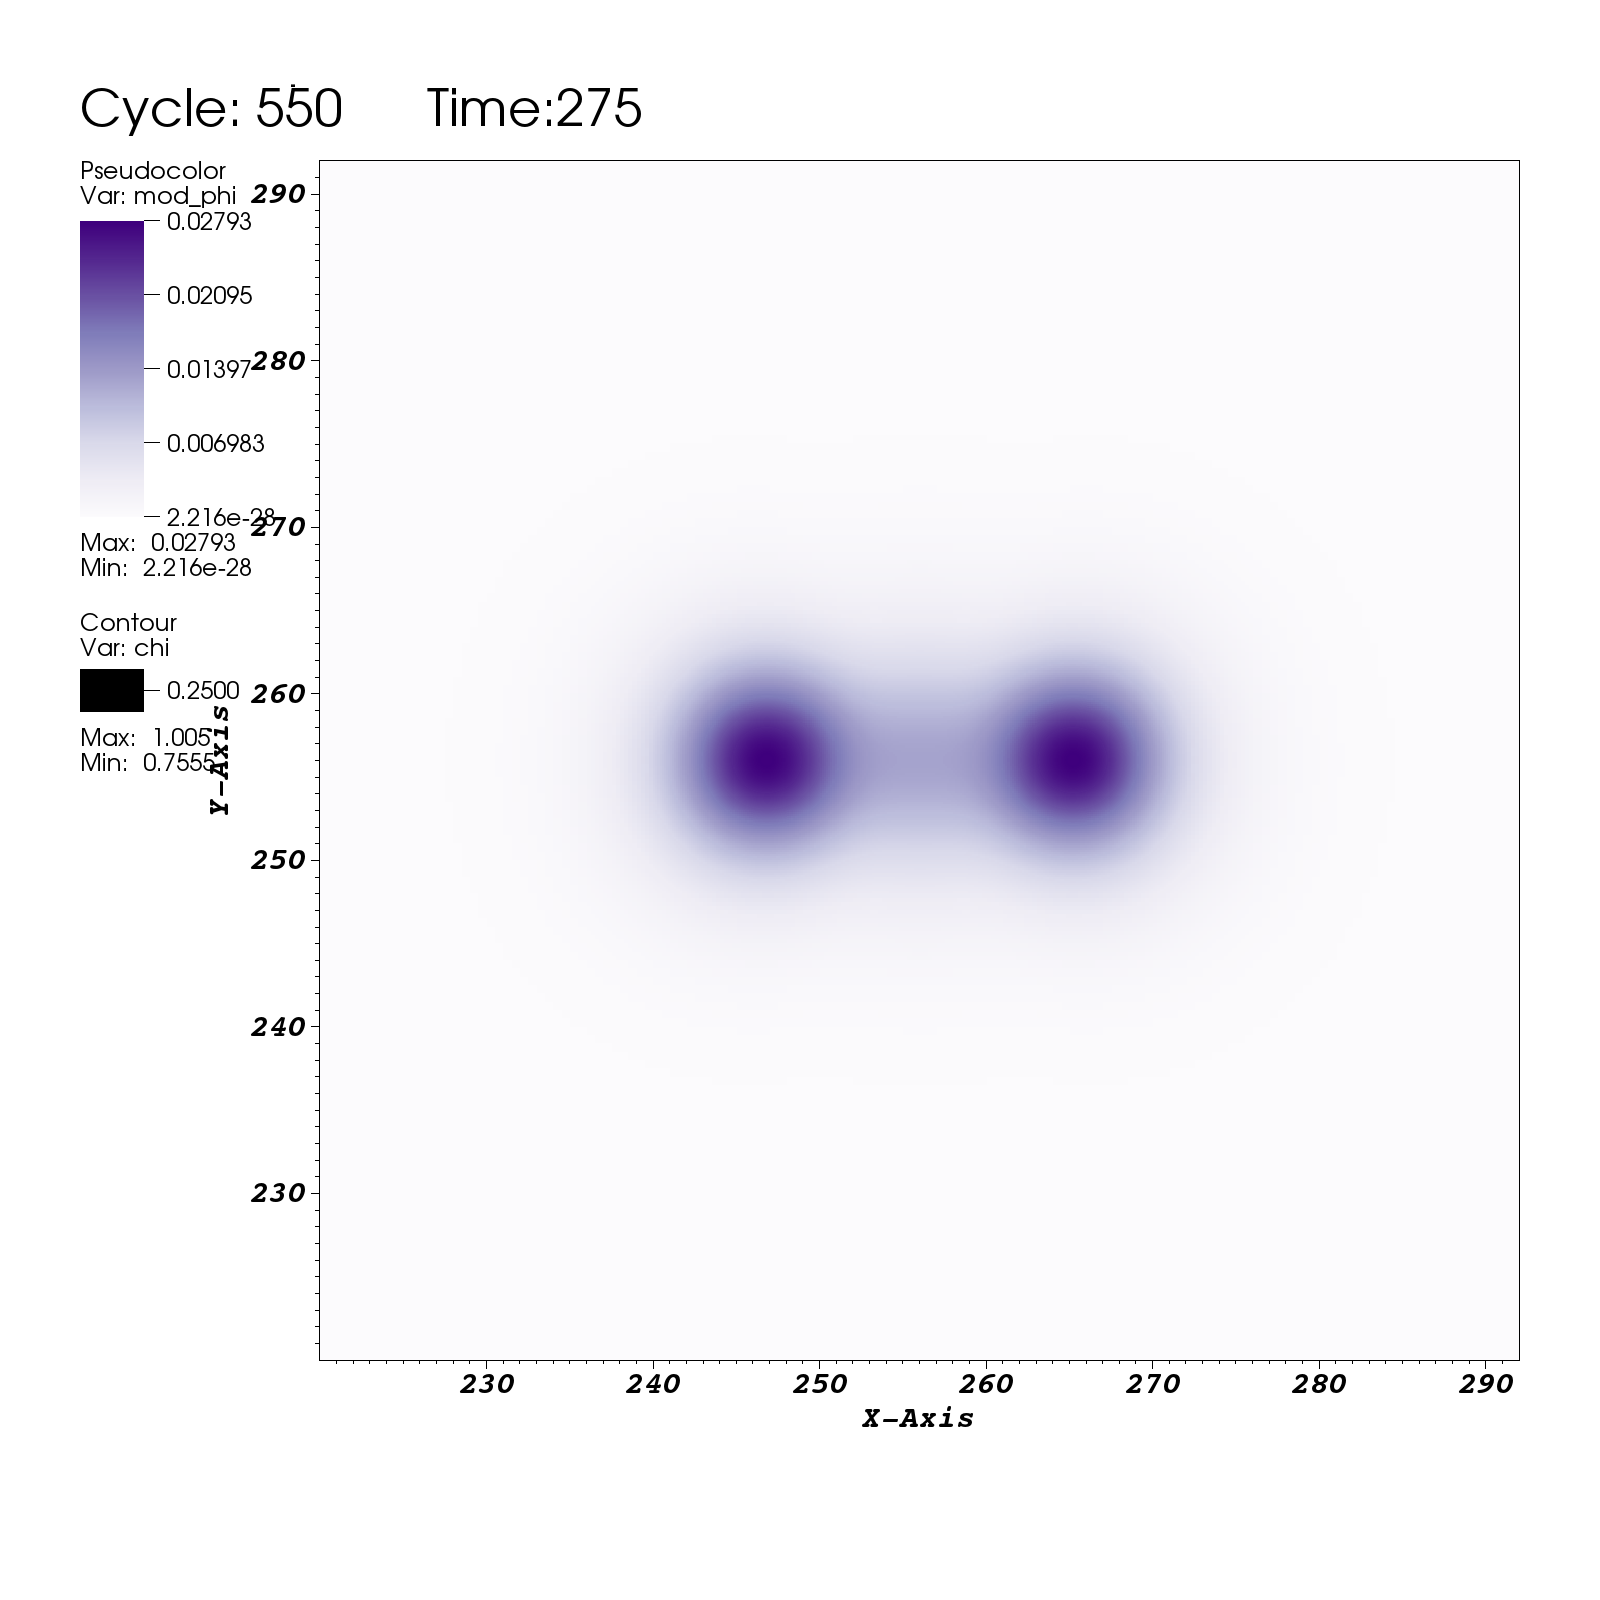
\includegraphics[width=0.50\textwidth]{modphi/headon_mod_phi0011.png}}\hfill
  \subfloat{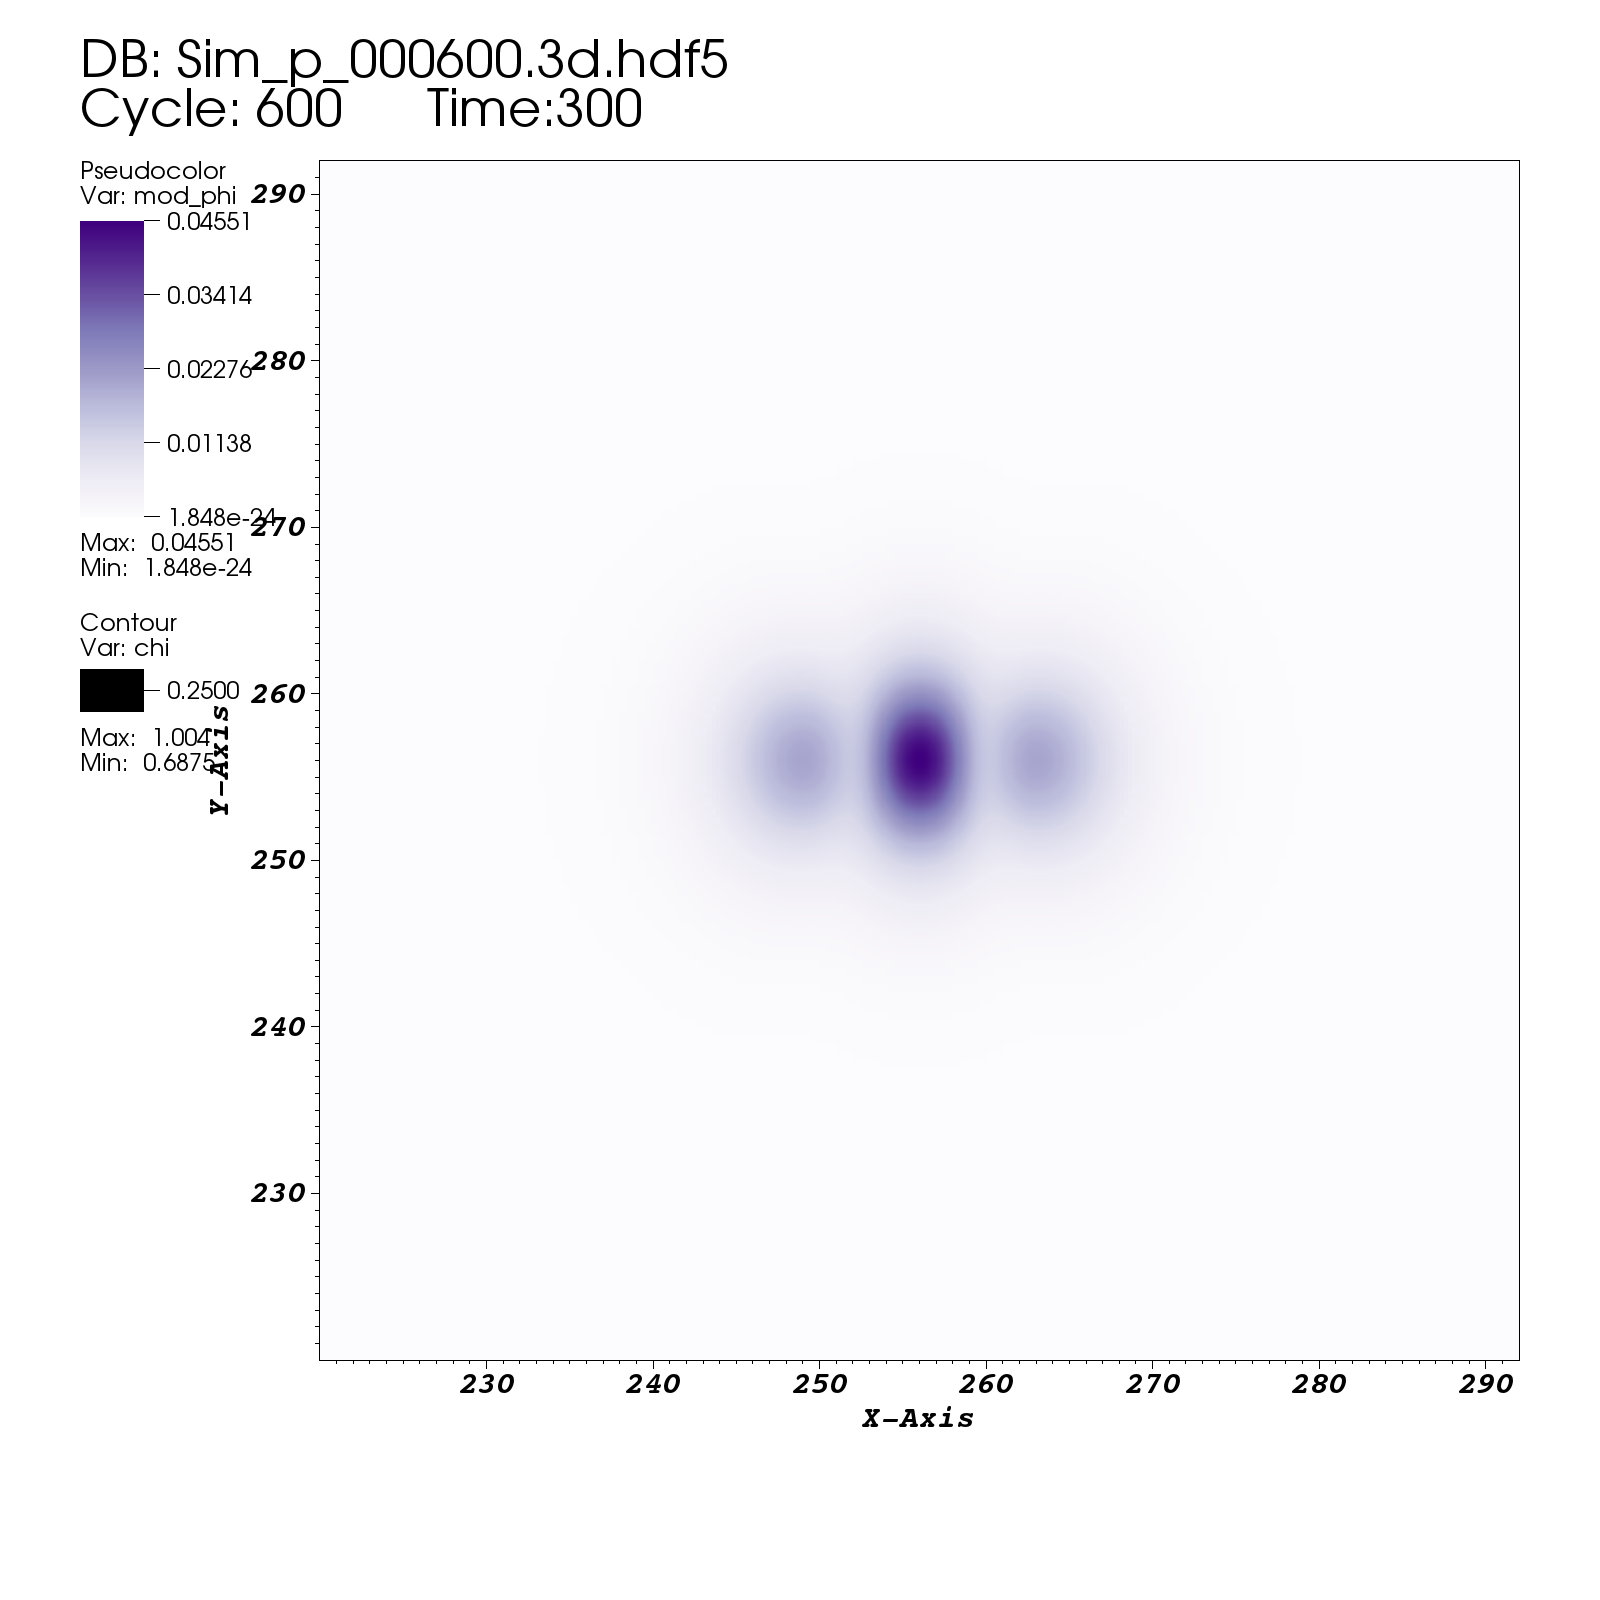
\includegraphics[width=0.50\textwidth]{modphi/headon_mod_phi0012.png}}
  \hspace{0 mm}
  \subfloat{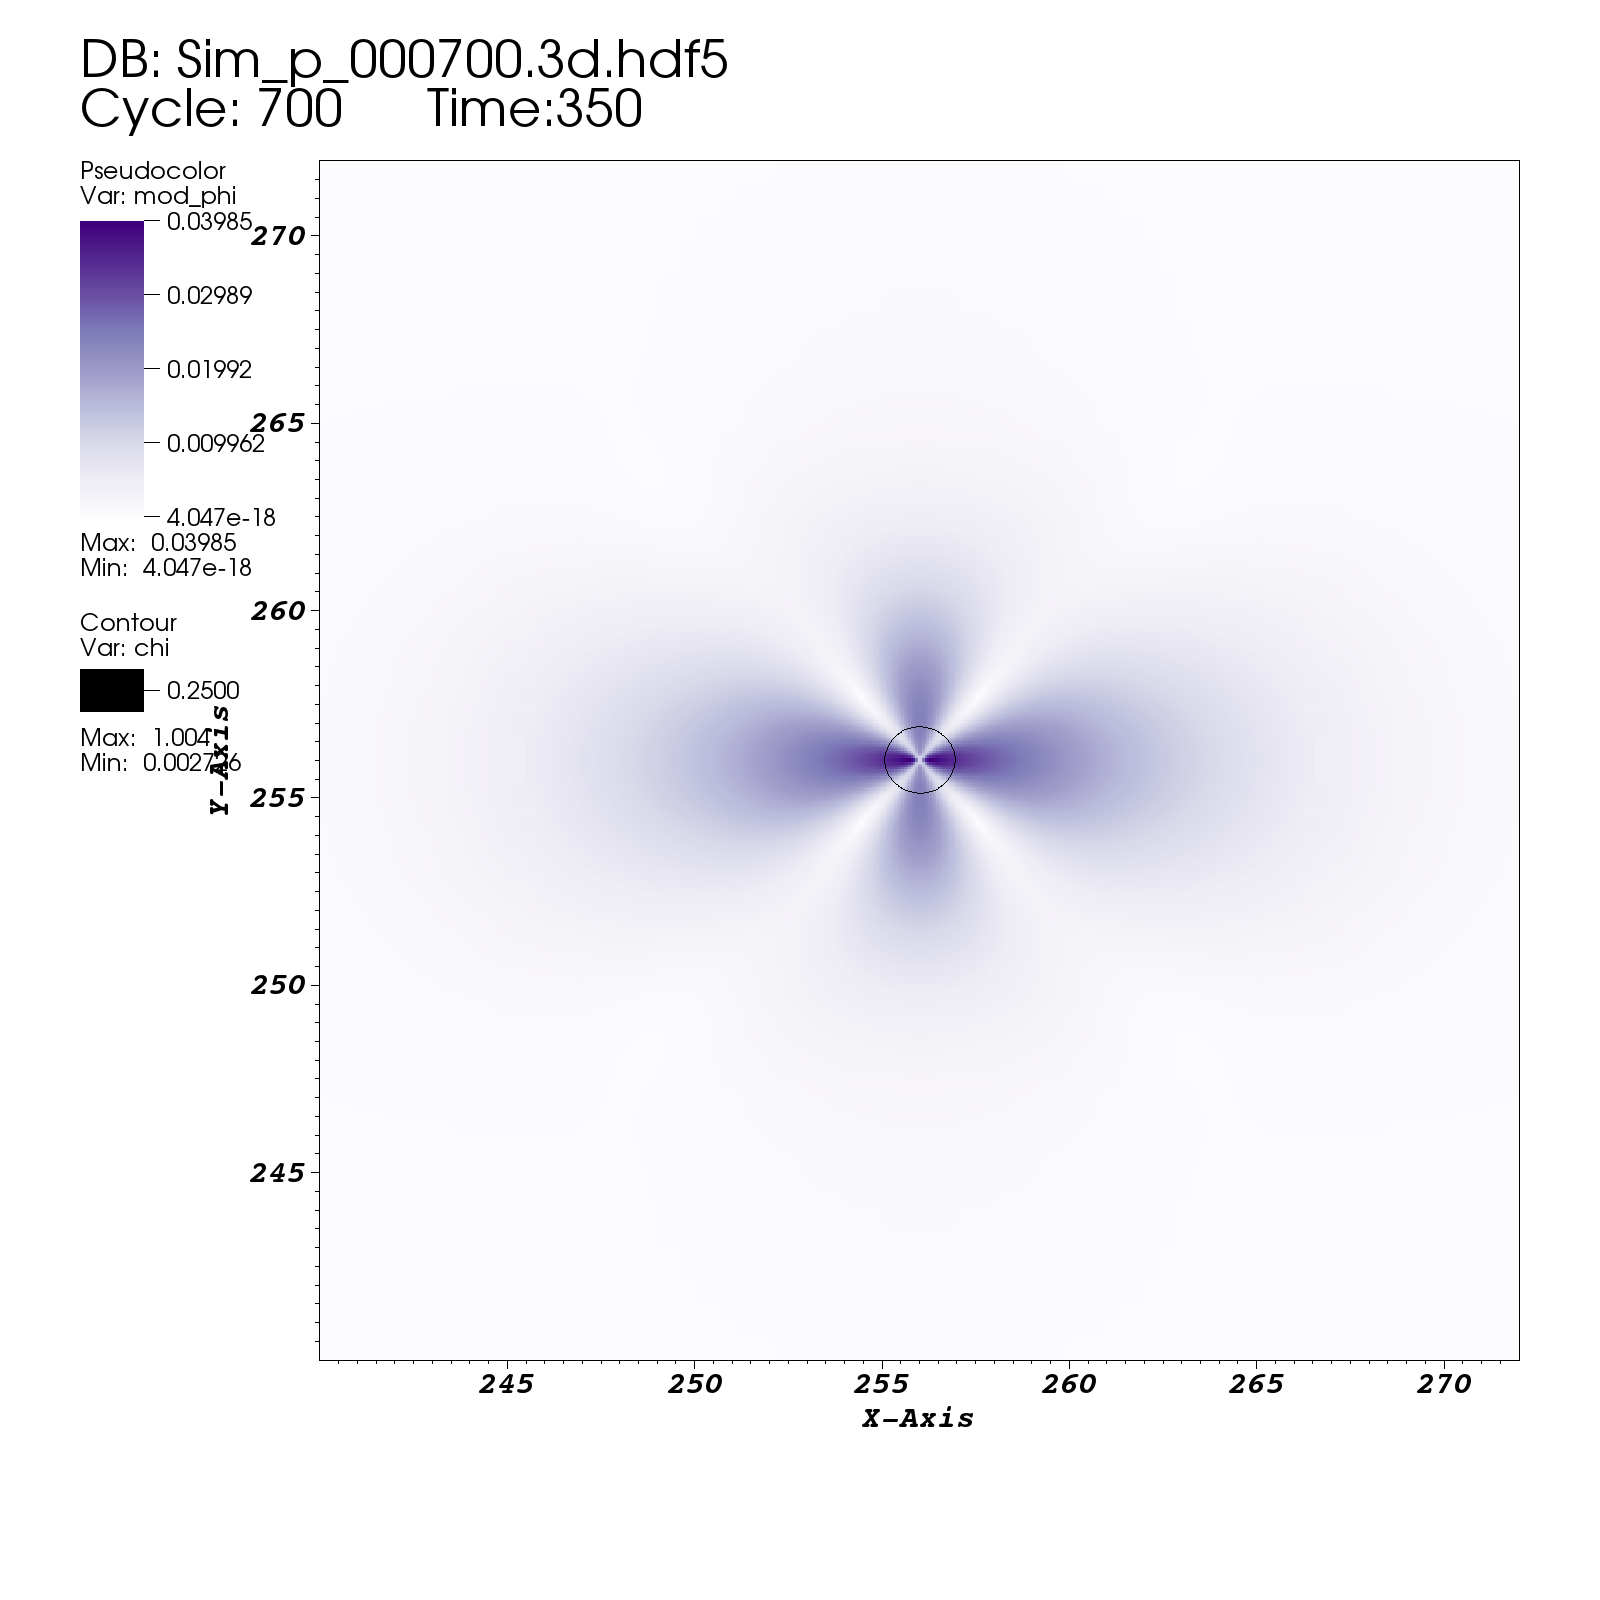
\includegraphics[width=0.50\textwidth]{modphi/headon_mod_phi0014.png}}\hfill
  \subfloat{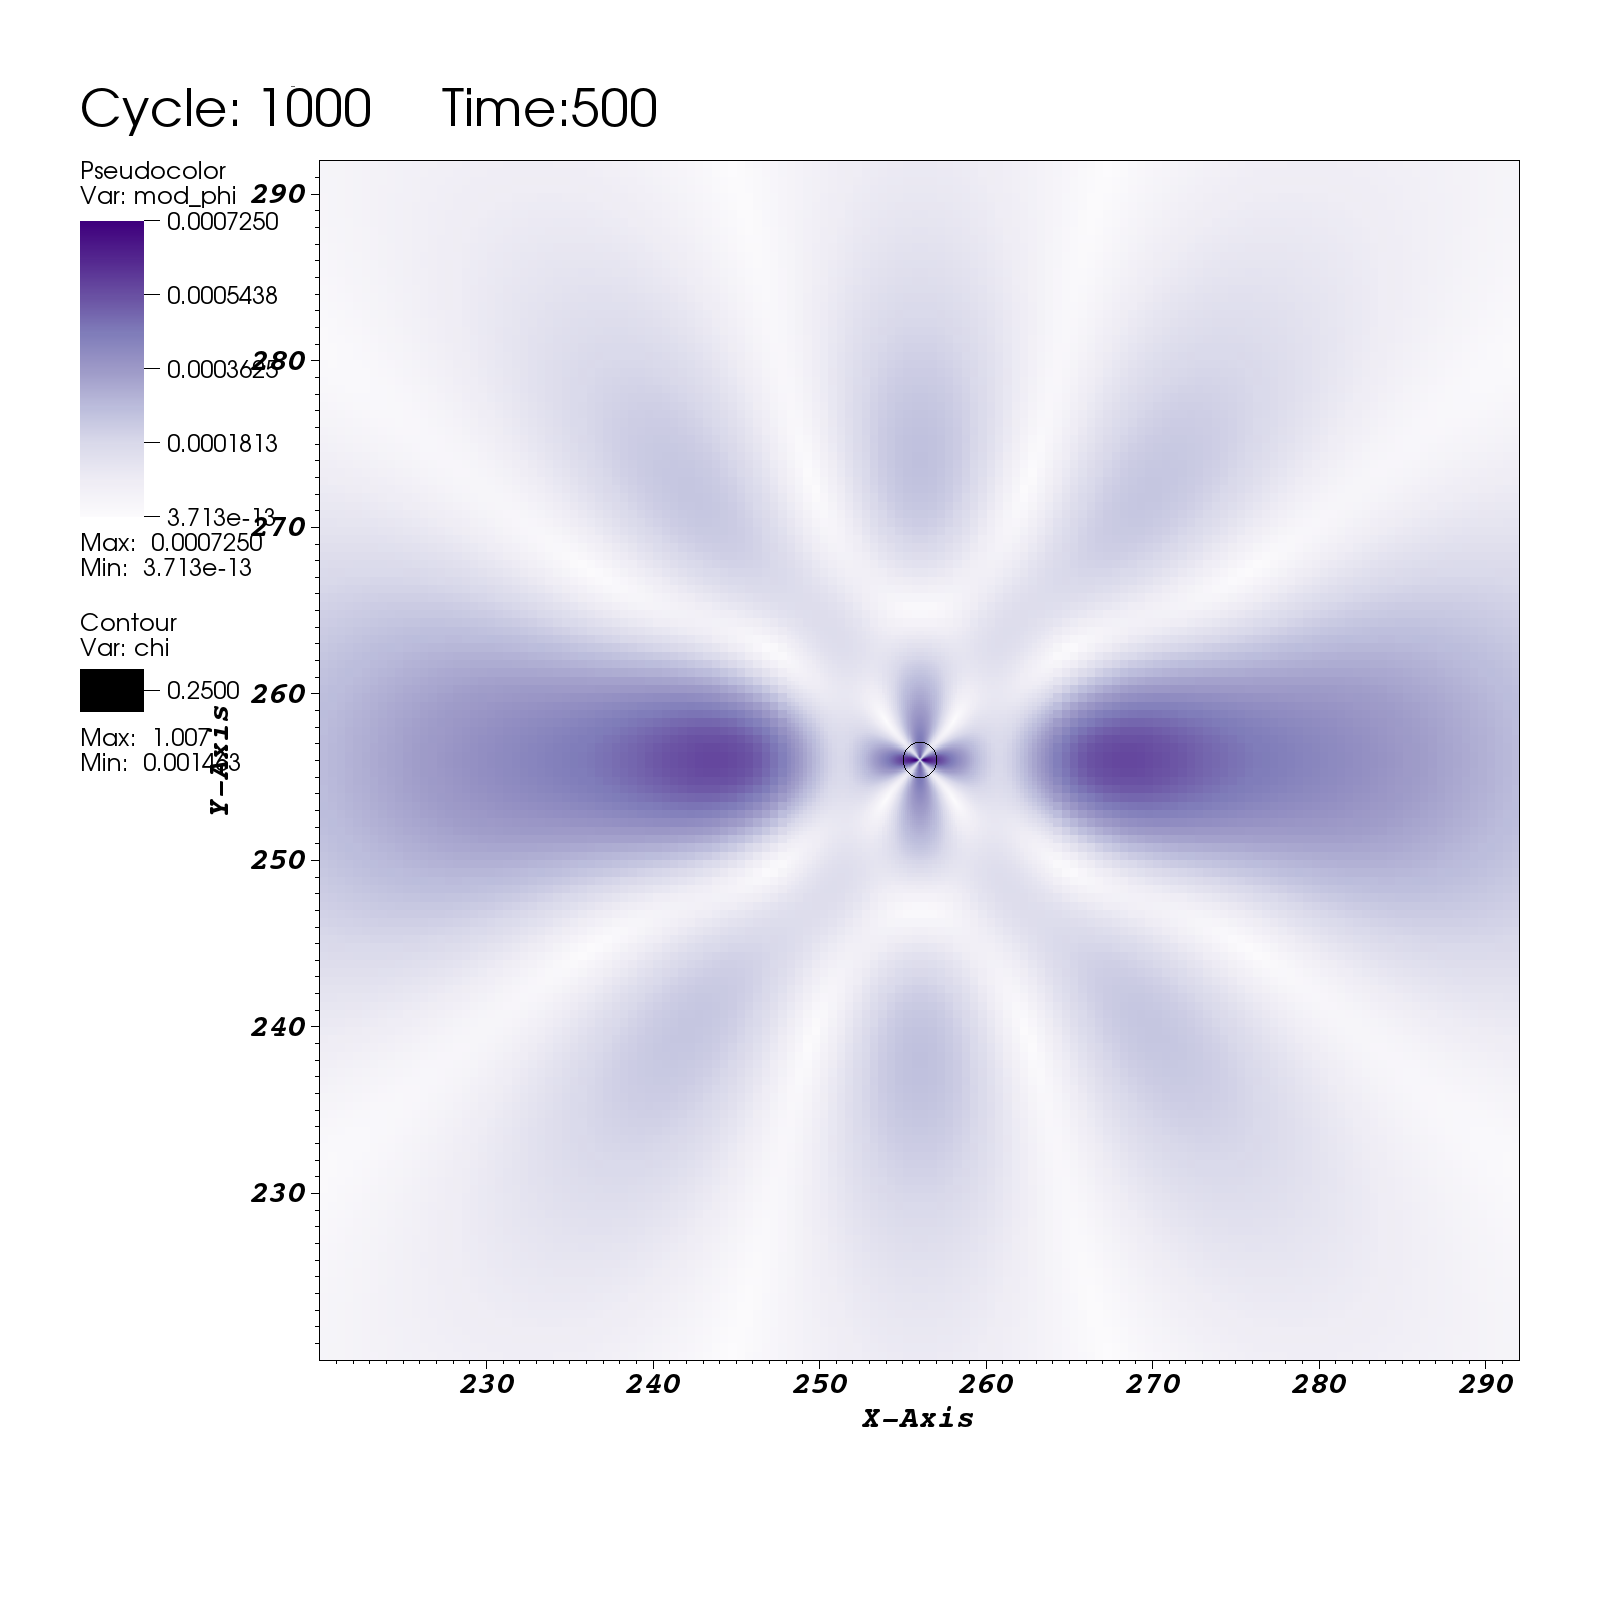
\includegraphics[width=0.50\textwidth]{modphi/headon_mod_phi0020.png}}
  \caption{Field plots of $|\vp|$ during evolution at four different times. Time $t=275~m^{-1}$ and $t=300~m^{-1}$ show snapshots momentarily before and after star collision. Time $t=350~m^{-1}$ shows the scalar field accreting into the recently formed black hole. Time $t= 500~m^{-1}$ shows the scalar field surrounding the black hole a little later; notably the amplitude is lower. Both the plots of $t=350~m^{-1}$ and $t=500~m^{-1}$ include a contour plot of $\chi=0.25$ acting as an approximate marker for the event horizon. The Newtonian estimate of collision time is $t= 287.6~m^{-1}$.}
  \label{boson:fig:ff7}
\end{figure}






\begin{figure}[h!]
\subfloat{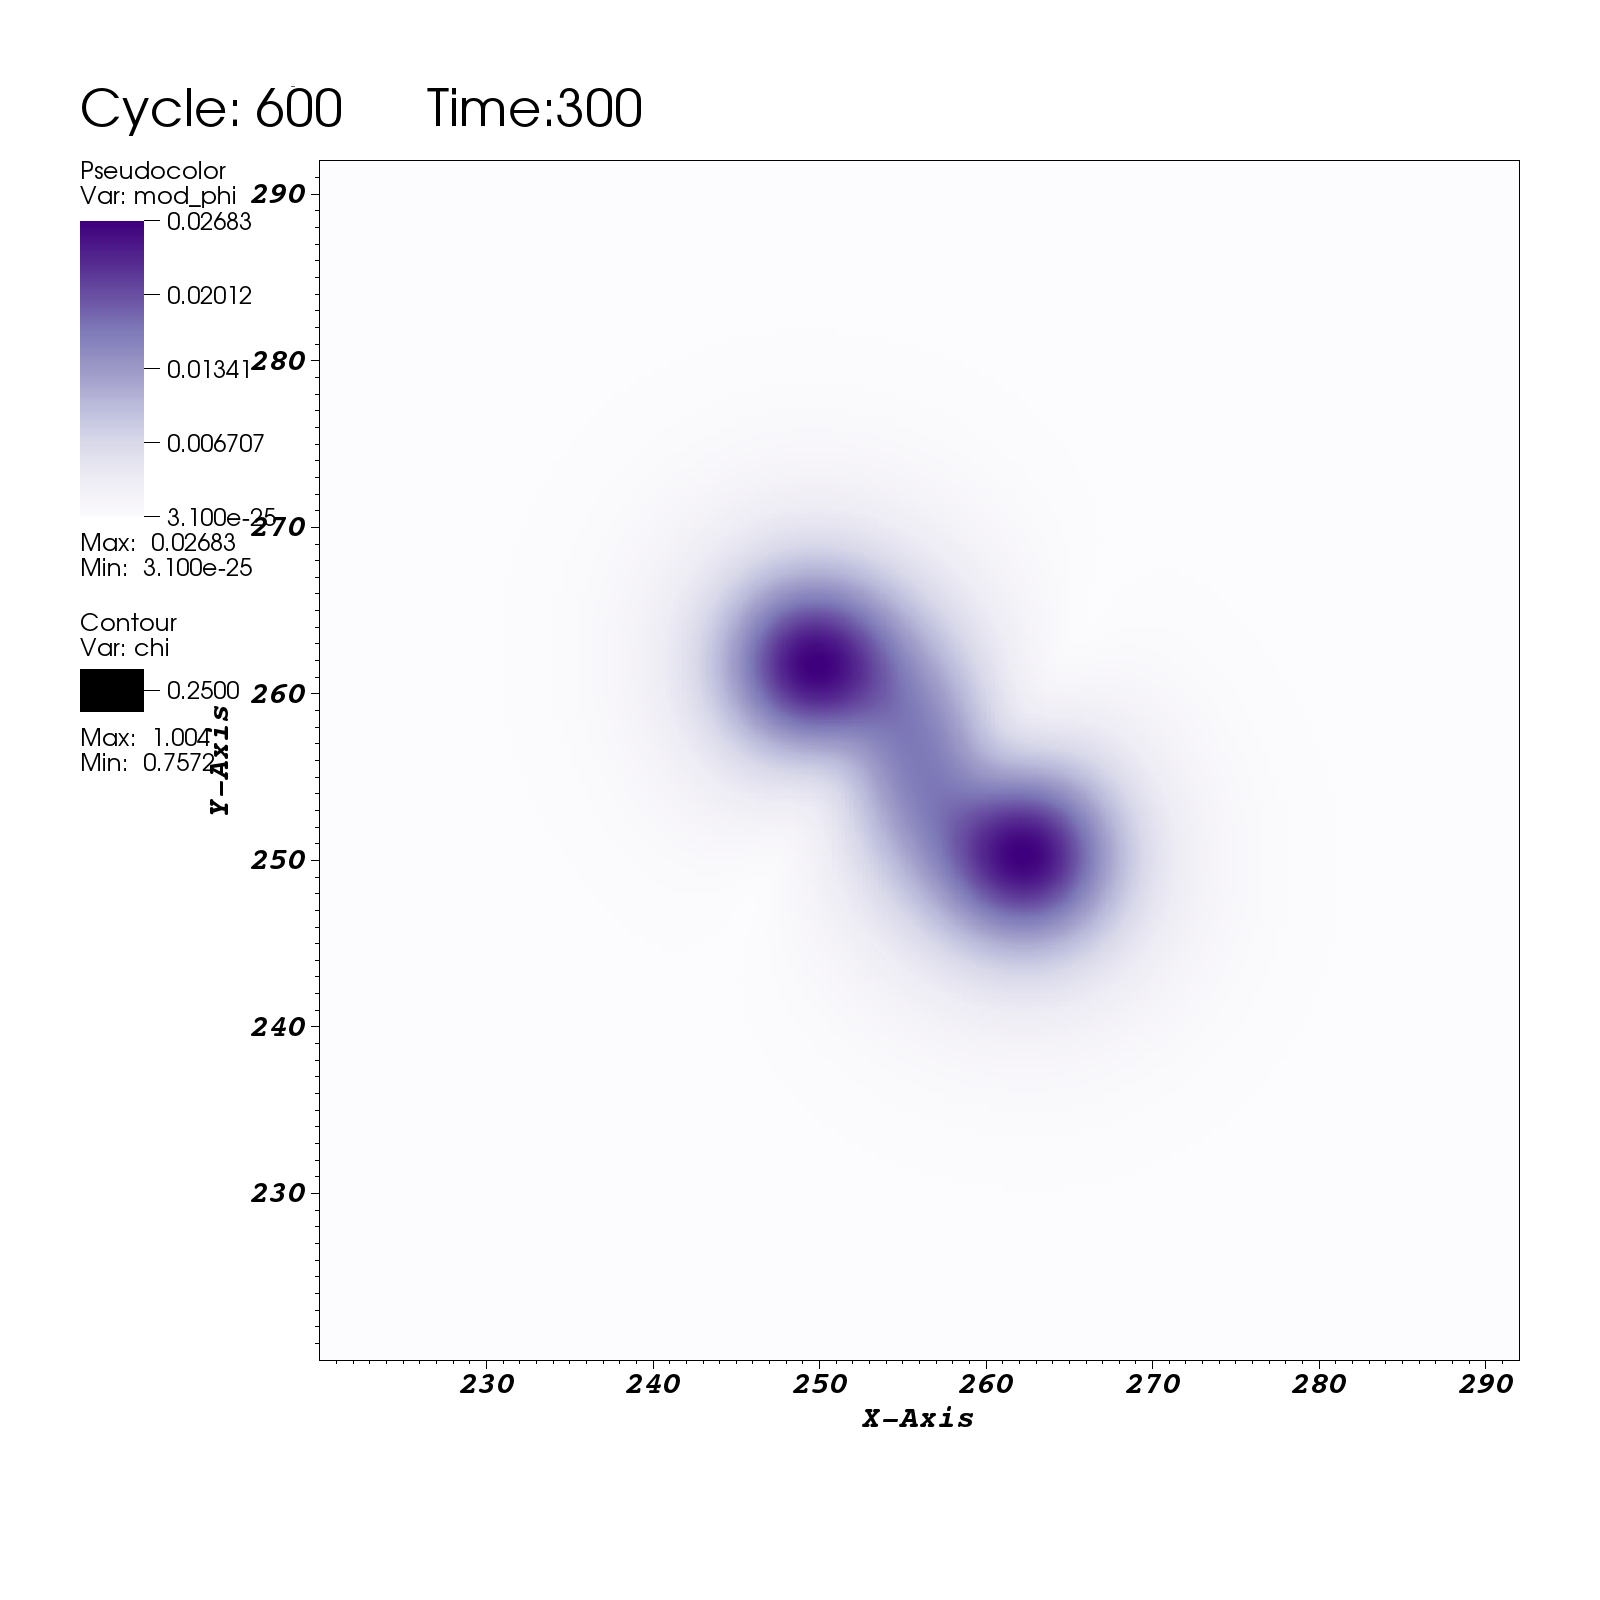
\includegraphics[width=0.5\textwidth]{modphi/graze_mod_phi0012.png}}\hfill
\subfloat{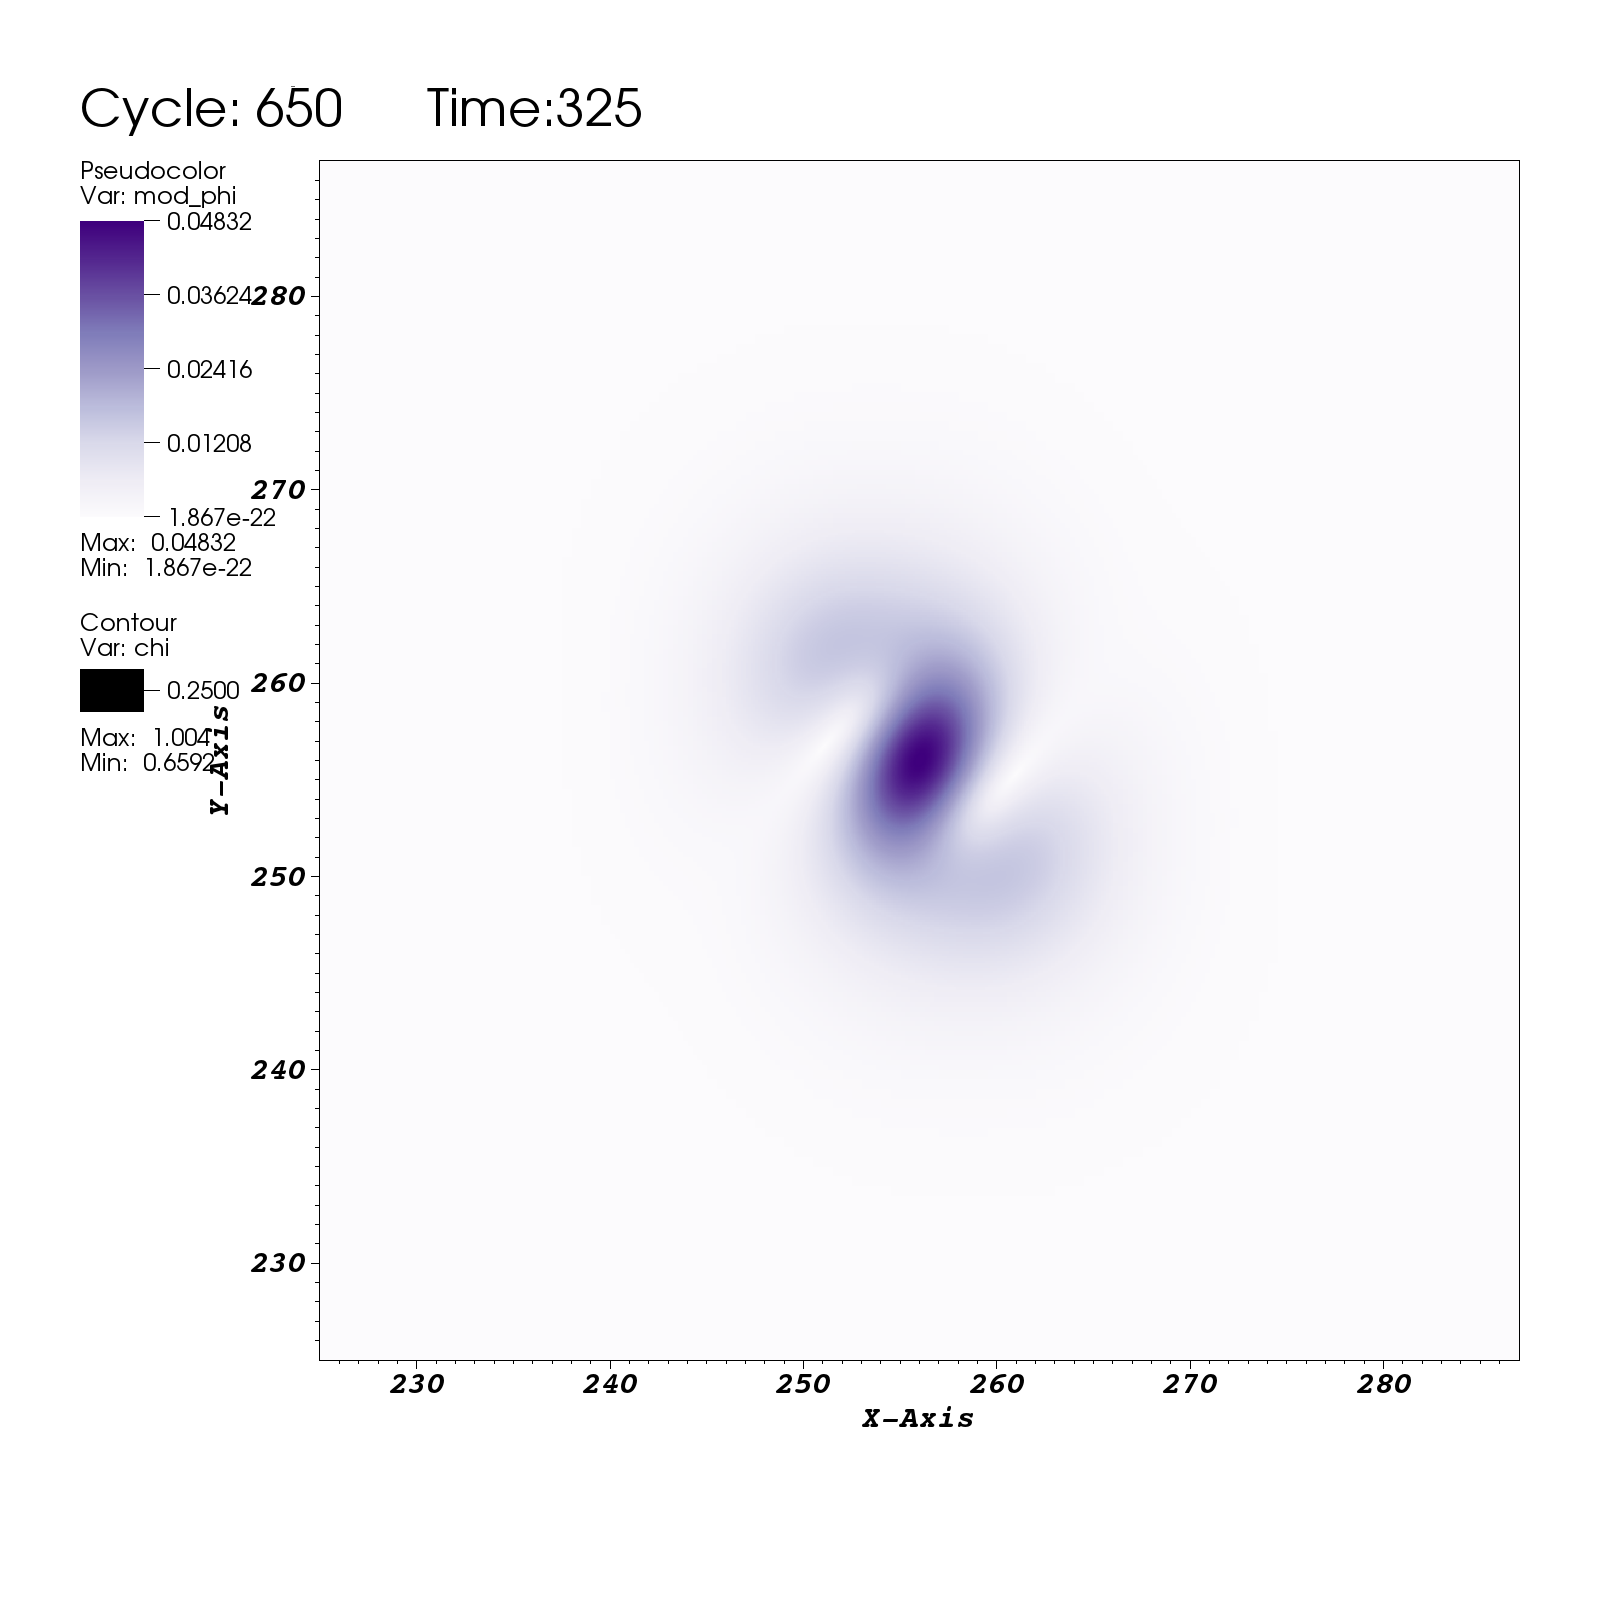
\includegraphics[width=0.5\textwidth]{modphi/graze_mod_phi0013.png}}
\hspace{0 mm}
\subfloat{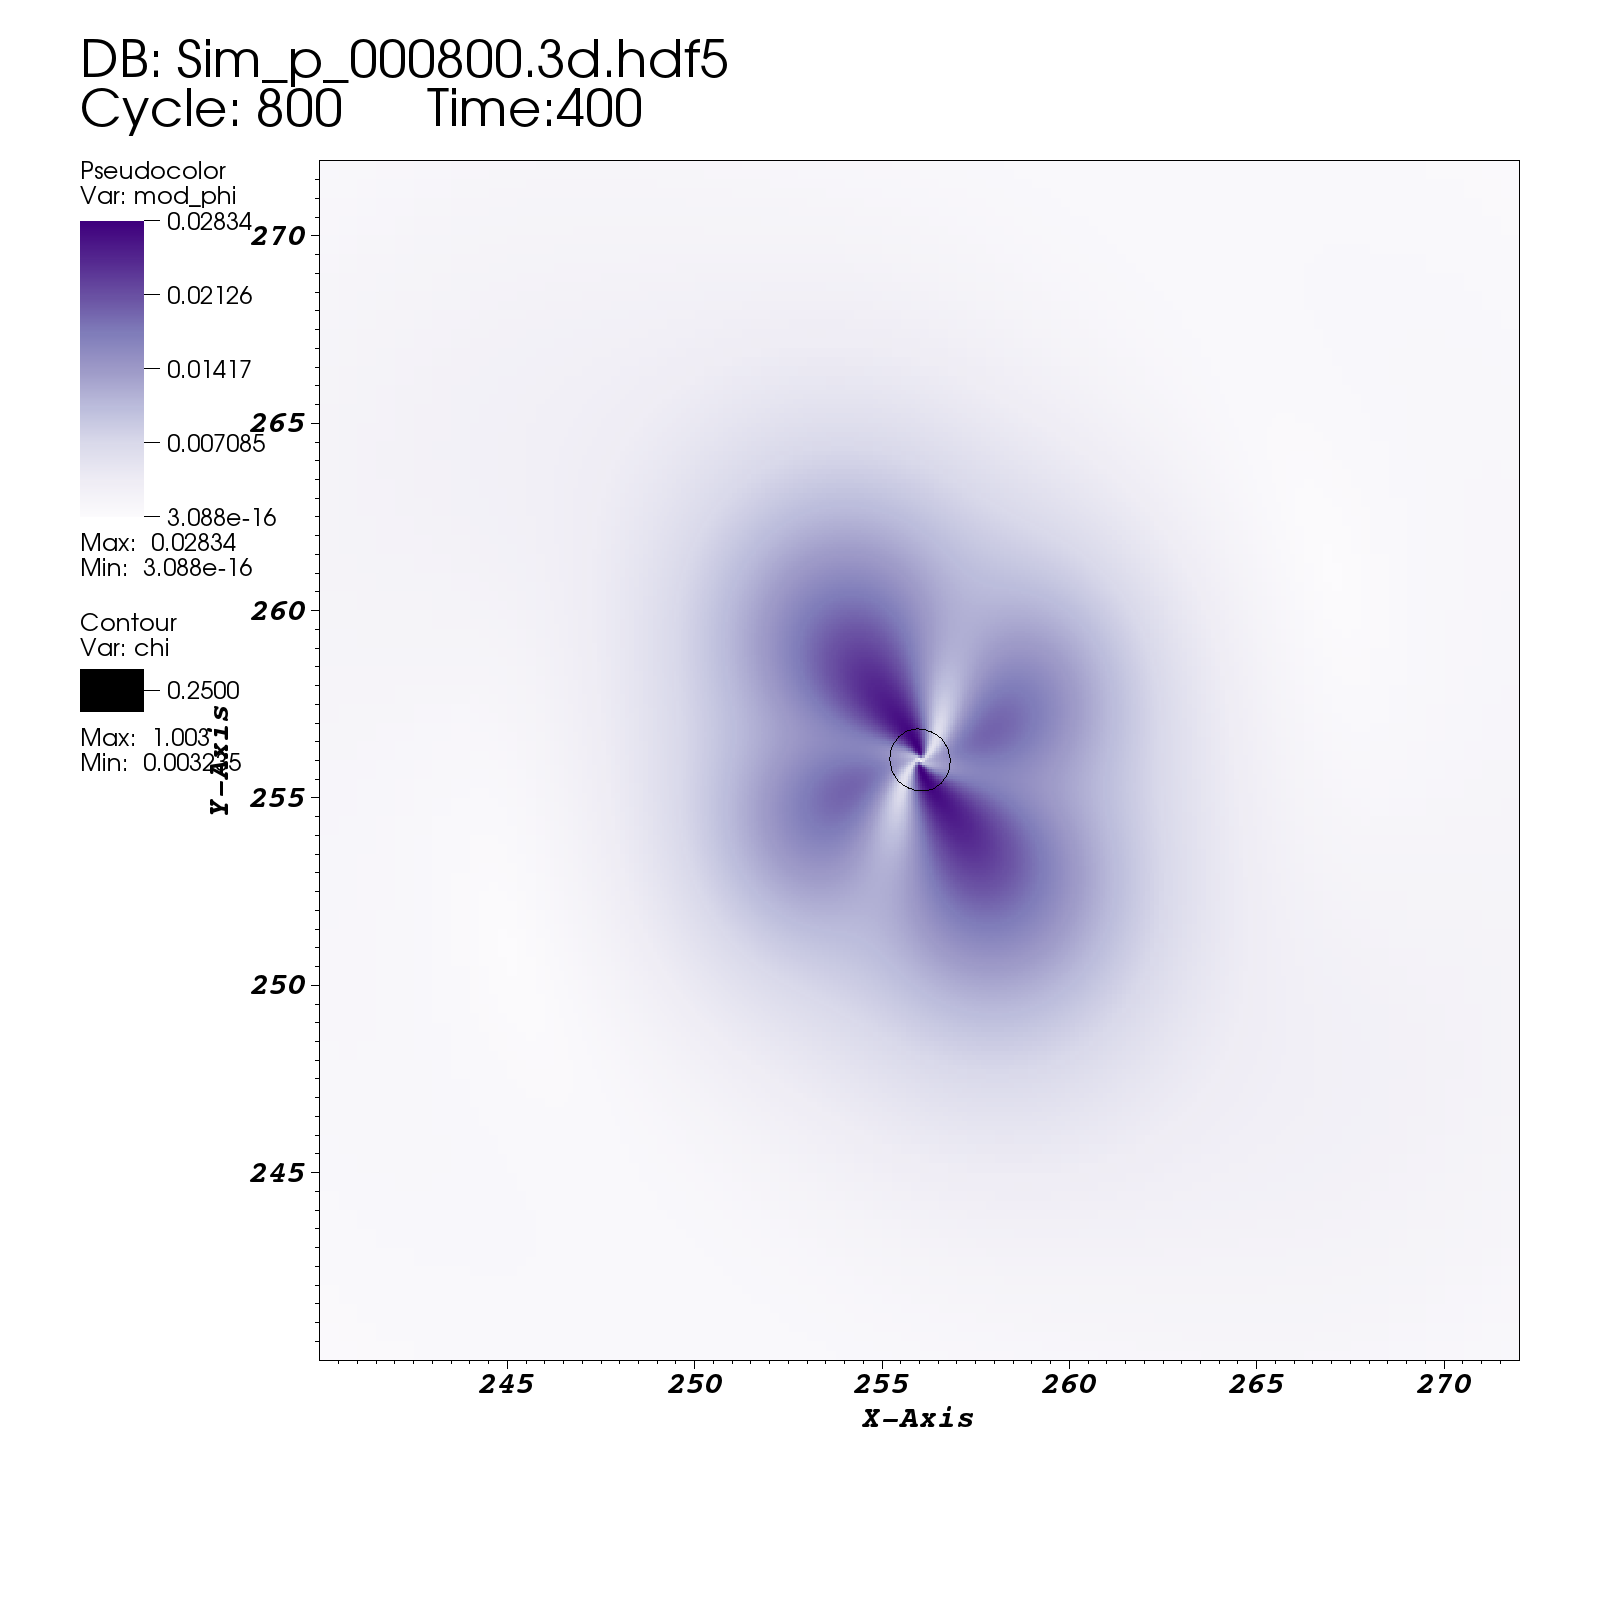
\includegraphics[width=0.5\textwidth]{modphi/graze_mod_phi0016.png}}\hfill
\subfloat{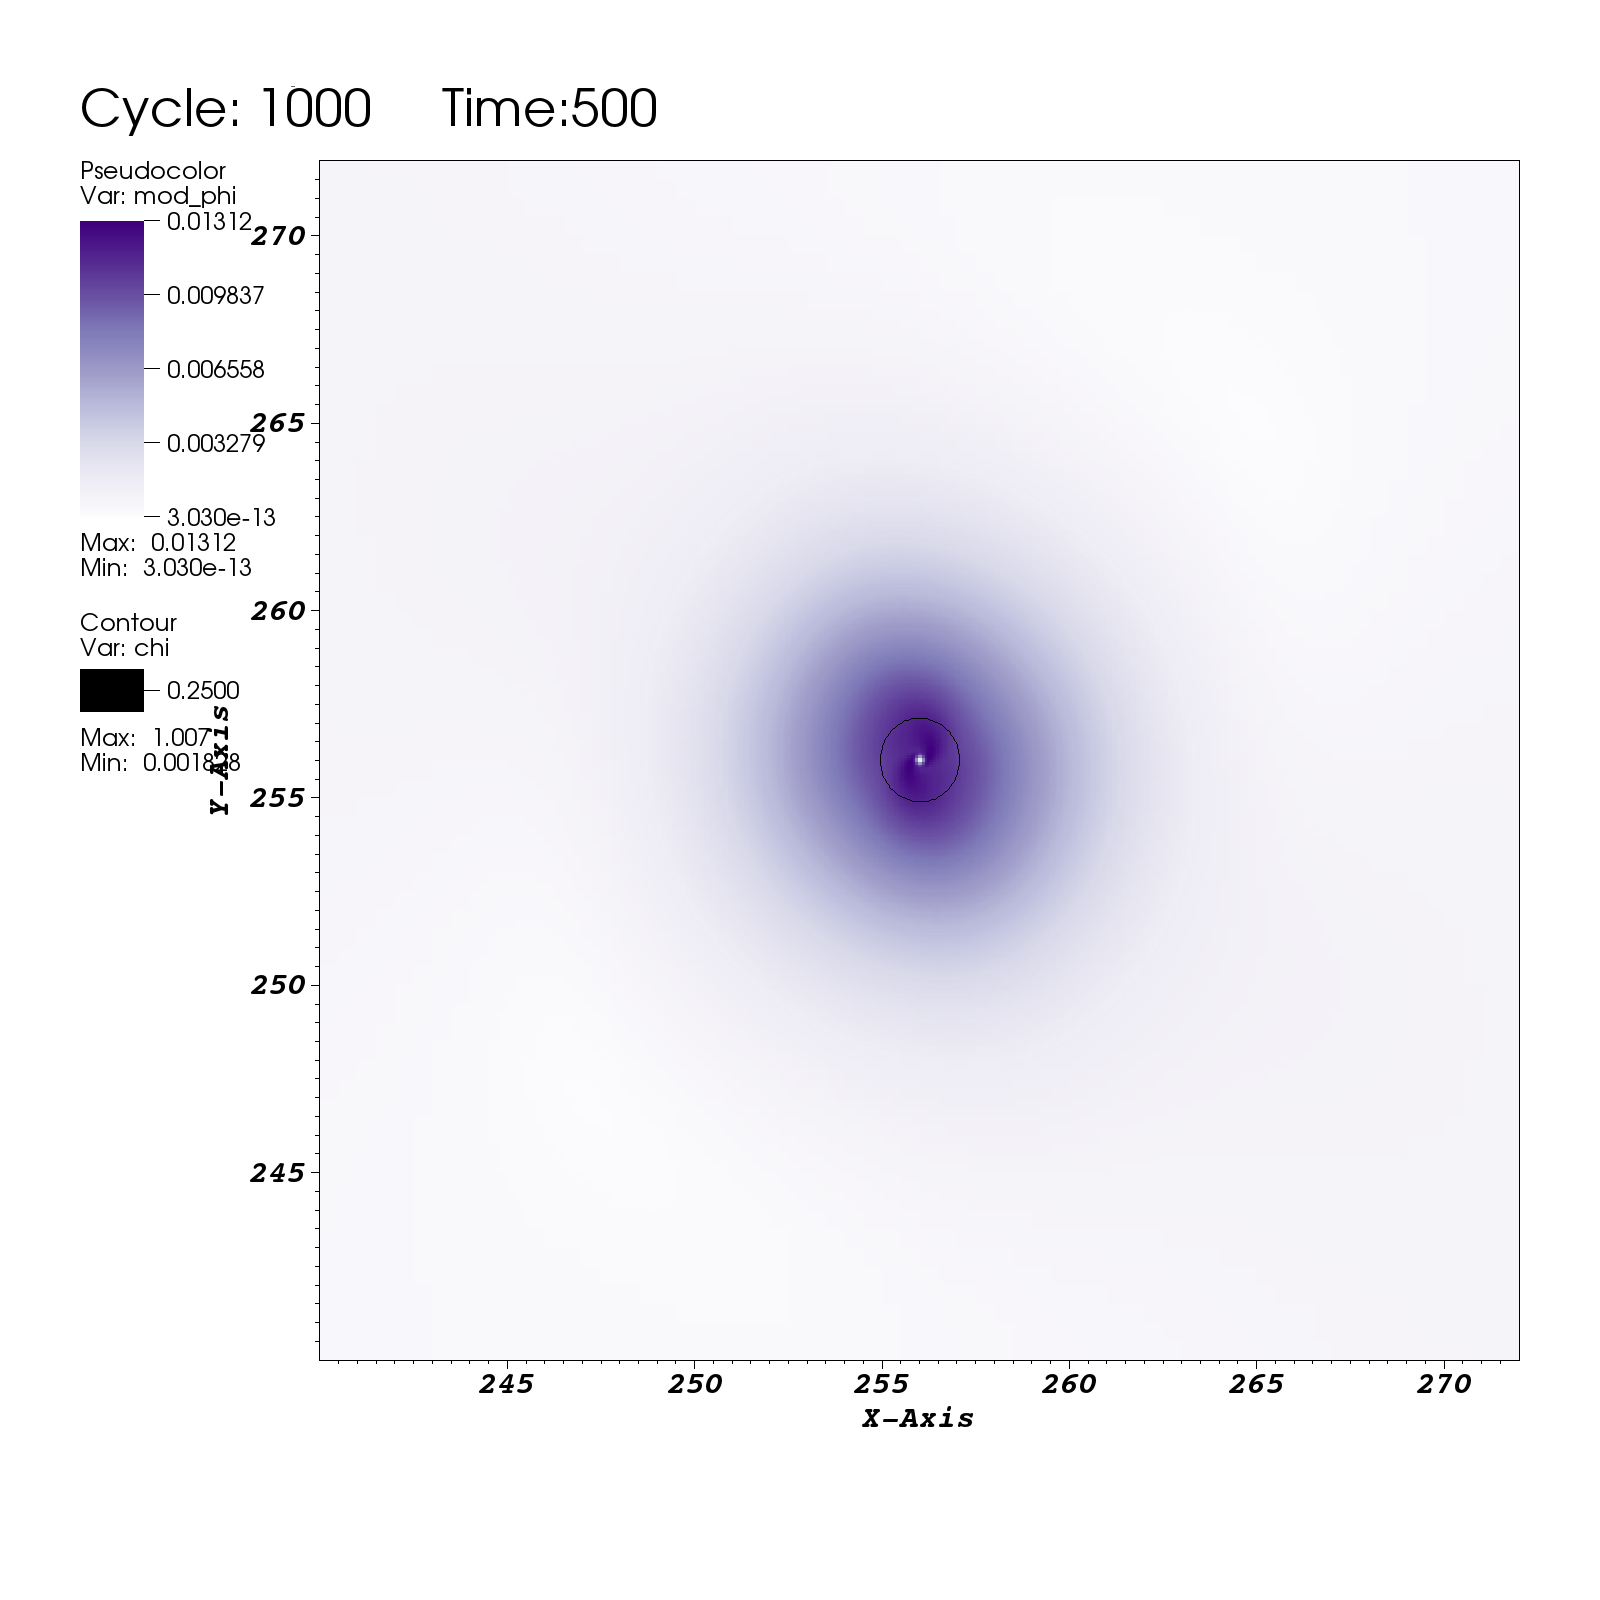
\includegraphics[width=0.5\textwidth]{modphi/graze_mod_phi0020.png}}
\caption{Field plots of $|\vp|$ during evolution at four different times for the grazing boson star collision. Time $t=300~m^{-1}$ and $t=325~m^{-1}$ show snapshots momentarily before and after the collision. The Newtonian estimate of collision time is $t= 315.8~m^{-1}$. Time $t=400~m^{-1}$ shows the scalar field accreting into the recently formed black hole. Time $t= 500~m^{-1}$ shows the scalar field surrounding the black hole a little later; here this is called a {\it toroidal wig}. Both the plots of $t=400~m^{-1}$ and $t=500~m^{-1}$ display a contour plot of $\chi=0.25$ acting as an approximate marker for the event horizon. }
\label{boson:fig:ff10}
\end{figure}



%BLACKHOLESBLACKHOLESBLACKHOLESBLACKHOLESBLACKHOLESBLACKHOLESBLACKHOLESBLACKHOLESBLACKHOLESBLACKHOLESBLACKHOLESBLACKHOLESBLACKHOLESBLACKHOLESBLACKHOLESBLACKHOLESBLACKHOLESBLACKHOLESBLACKHOLESBLACKHOLESBLACKHOLESBLACKHOLESBLACKHOLESBLACKHOLESBLACKHOLESBLACKHOLESBLACKHOLESBLACKHOLESBLACKHOLESBLACKHOLESBLACKHOLESBLACKHOLESBLACKHOLESBLACKHOLESBLACKHOLESBLACKHOLESBLACKHOLESBLACKHOLESBLACKHOLESBLACKHOLESBLACKHOLESBLACKHOLESBLACKHOLESBLACKHOLESBLACKHOLESBLACKHOLESBLACKHOLESBLACKHOLESBLACKHOLESBLACKHOLESBLACKHOLESBLACKHOLESBLACKHOLESBLACKHOLESBLACKHOLESBLACKHOLESBLACKHOLESBLACKHOLESBLACKHOLESBLACKHOLESBLACKHOLESBLACKHOLESBLACKHOLESBLACKHOLES


% \subsection{Collisions of Boson Stars with Black Holes} \label{grchombo:sec:bsbhcollisions}

% Here the headon and grazing collisions of a boson star with a black hole are presented. The superposition scheme is given in section \ref{grchombo:sec:superposition}. Similarly to the previous section on the collision of two identical stars, the star and black hole mass are identical, each with an ADM mass $M=0.532(7)$. The black hole and star are placed at positions $\pm\{40,0,0\}$ in the headon case and $\pm\{40,8,0\}$ in the grazing case and are boosted together with respective velocities $\mp\{0.1,0,0\}$ corresponding to a rapidity of $\psi=0.1003353$ (4 s.f.). The simulations have a physical domain size $L=512$ with $N=256$ gridpoints on AMR level zero, this gives a coarse grid resolution of $\Delta x = 2$. There are up to five extra AMR levels giving a finest grid resolution of $\Delta x = 16$.

% \subsubsection{Headon Collision}
%  \begin{figure}[h!]
%   \caption{Left: Maximum of $|\vp|$ during evolution, Right: Total integrated Noether charge $N$.}
%   \centering
%   \subfloat{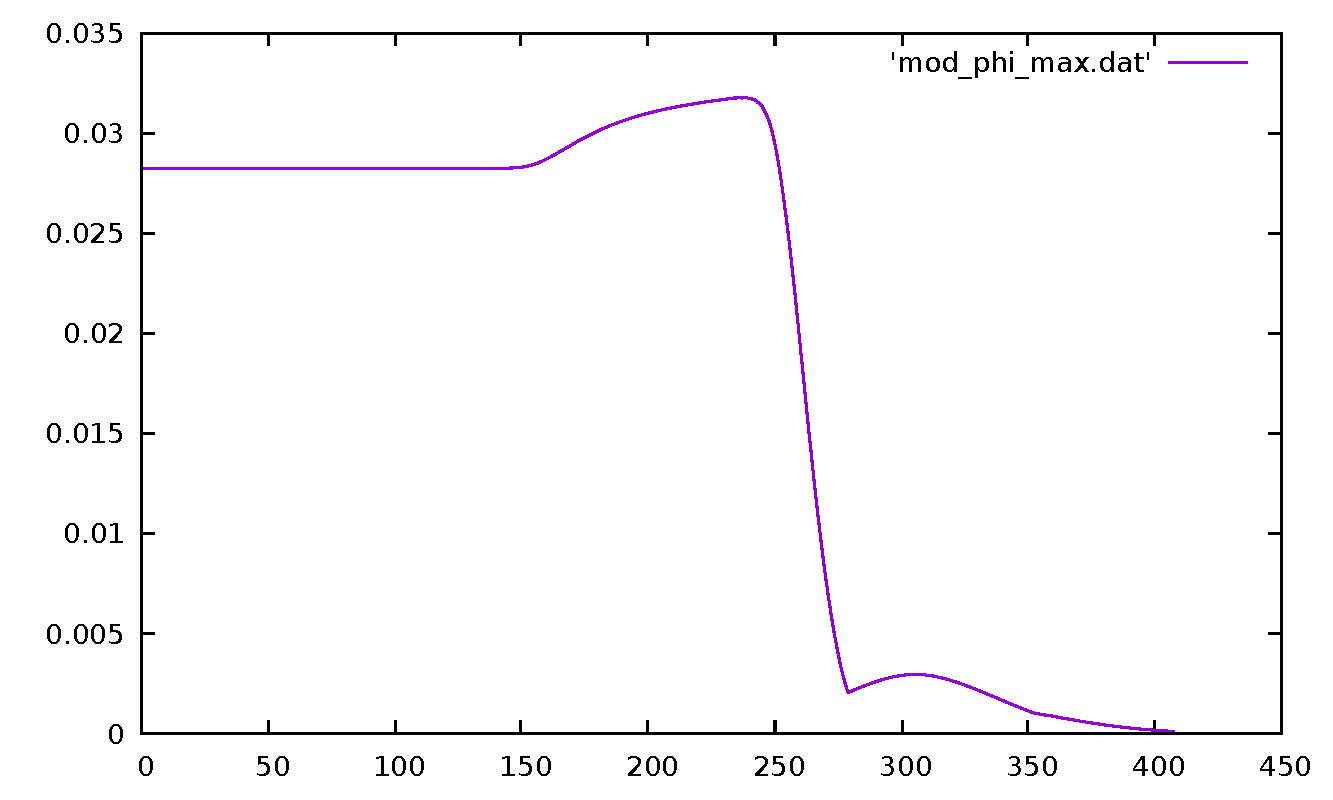
\includegraphics[width=0.5\textwidth]{data/headon_bhbs_modphi.pdf}\label{boson:fig:f12}}
%   \hfill
%   \subfloat{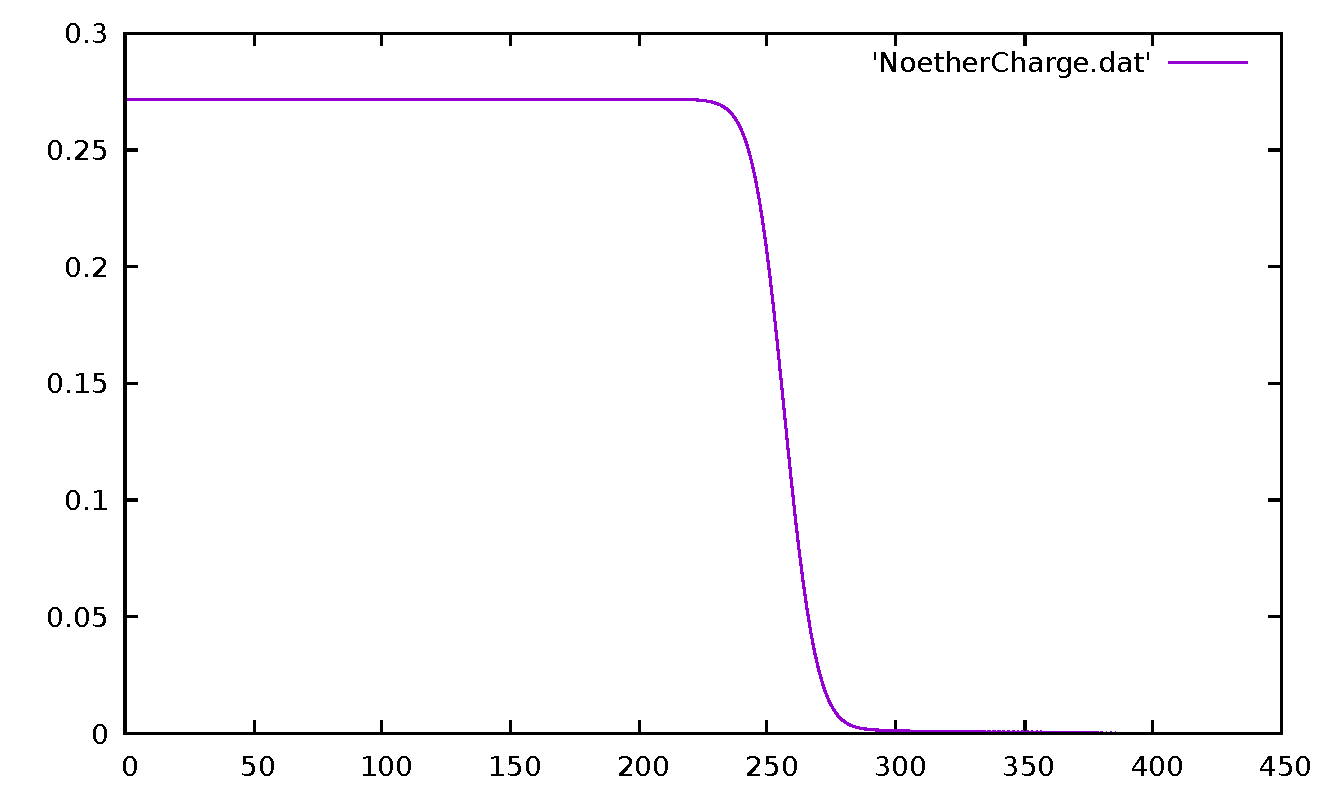
\includegraphics[width=0.5\textwidth]{data/headon_bhbs_n.pdf}\label{boson:fig:f13}}
% \end{figure}

% Figure (\ref{boson:fig:f7}) shows $|\vp|_{\rm max}$, the global maximum value of $|\vp|$, and the total Noether charge as a function of time for the headon collision. At time $t\approx 289 \cdot m$, $|\vp|_{\rm max}$ rapidly increases; a black hole is then formed. At time $t\approx 327 \cdot m$, $|\vp|_{\rm max}$ there is a temporal maximum in $|\vp|_{\rm max}$ as the resolution limit of the simulation is reached and the scalar field is damped away by the Kreiss-Oliger dissipation mentioned in section \ref{grchombo:sec:grchombo}. This damping can also be seen in the Noether charge plot, at a time of $t \approx 326 \cdot m$, where the total charge that should remain constant falls. The lack of sufficient resolution inside the black hole is not disasterous to the external simulation fortunately; the erorrs accumulated are trapped inside the event horizon.

% The gravitational wave extraction at radius $r=140 \cdot m$ is given in figure \ref{boson:fig:f9}. A spin-weighted spherical harmonic decomposition of the Newman-Penrose scalar $\Psi_4$ [REF] has been done and the $m,l = 2,0$ and $m,l = 2,2$ modes are plotted.

% \begin{figure}[h!]
%   \caption{Left: Maximum of $|\vp|$ during evolution, Right: Total integrated Noether charge $N$.}
%   \centering
%   \subfloat{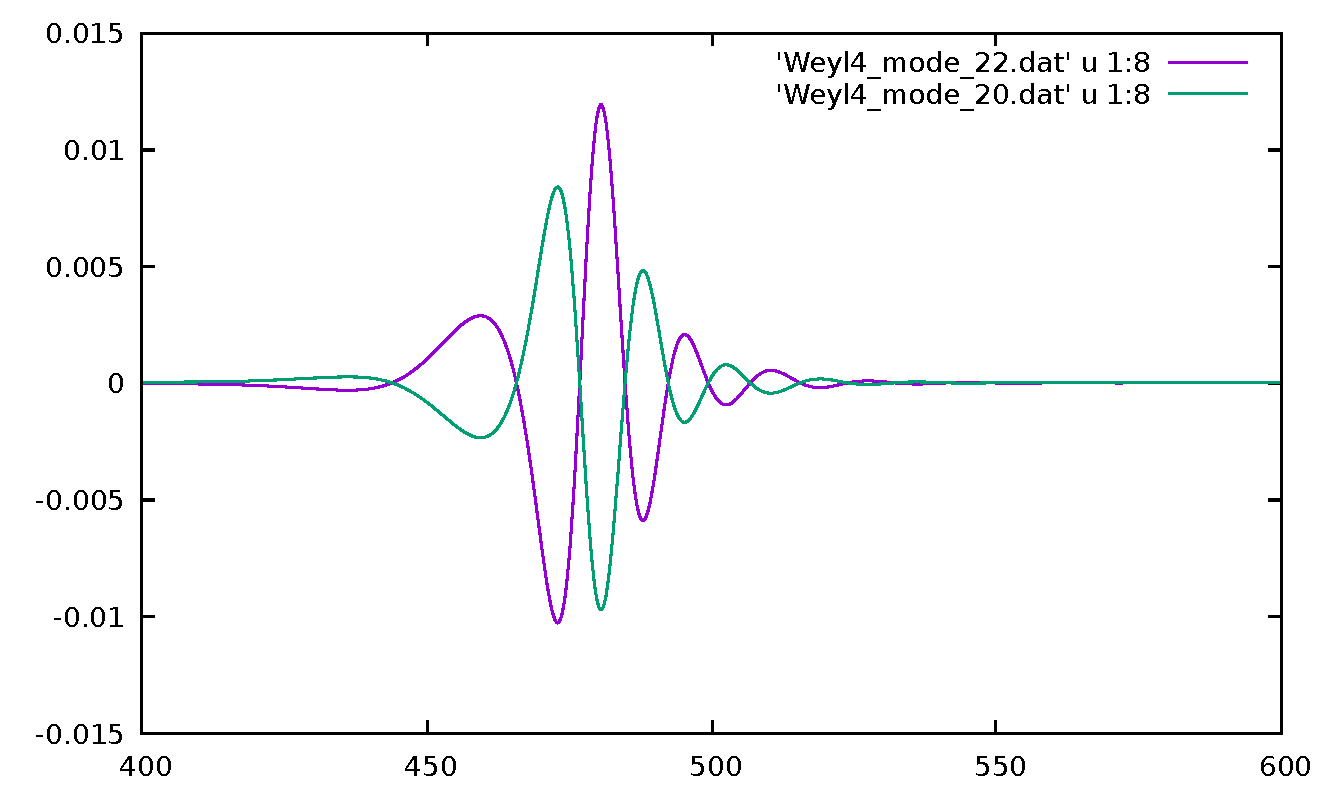
\includegraphics[width=0.5\textwidth]{data/headon_weyl22.pdf}\label{boson:fig:f14}}
% \end{figure}



% The dynamics of the two boson stars are shown in Fig.~(\ref{boson:fig:ff7}) plotting the scalar field modulus $|\vp|$ on the $x,y$ plane. The stars collide at at time $275\cdot m < t < 300 \cdot m$ and soon after an overdensity of scalar field forms collapsing to a black hole. This black hole subsequently accretes the surrouding scalar field; Fig.~(\ref{boson:fig:f7}) shows that the total Noether charge rapidly decays to zero as it falls into the black hole and is dissipated due to finite resolution effects. MAYBE DONT PUT THIS TWICE?

% as can be seen from the remnannt moving in (cvia coordinates) the simaultion is not in the rest frame.







%  \begin{figure}[h!]
%   \caption{Field plots of $|\vp|$ during evolution at four different times. Time $t=200 \cdot m$ and $t=250 \cdot m$ show snapshots momentarily before and after the collision. Time $t=300 \cdot m$ shows the scalar field accreting into the black hole and time $t= 400 \cdot m$ shows the scalar field surrounding the black hole a little later; noteably the amplitude is lower. All plots have a contour plot of $\chi=0.25$ acting as a very approximate marker for the event horizon. The Newtonian estimate of collision time is $t= 287.6 \cdot m$.}
%   \subfloat{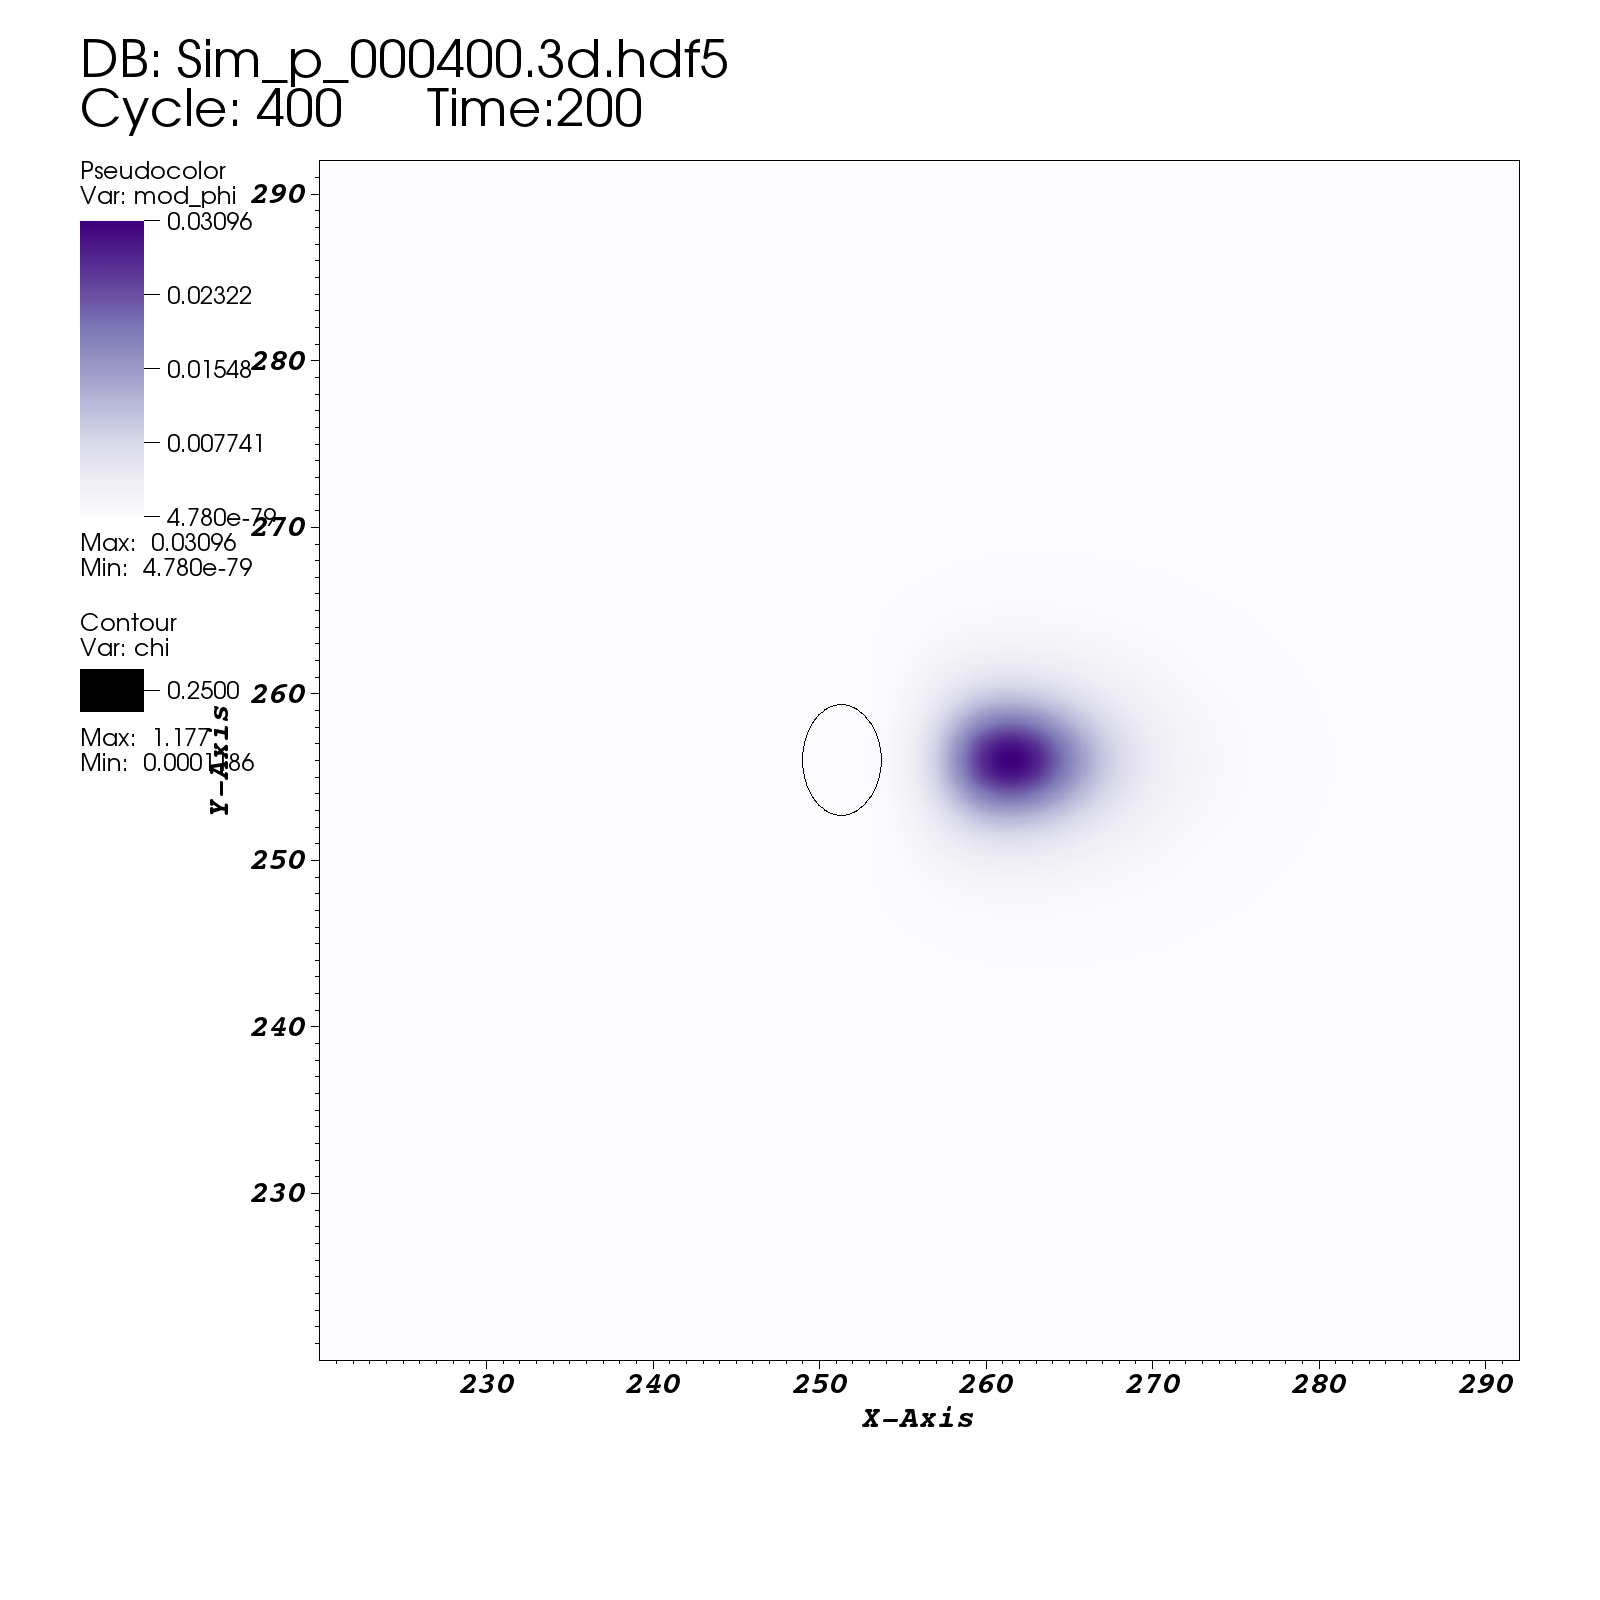
\includegraphics[width=0.45\textwidth]{modphi/headon_bhbs_mod_phi0008.png}\label{boson:fig:ff12}}
%   \subfloat{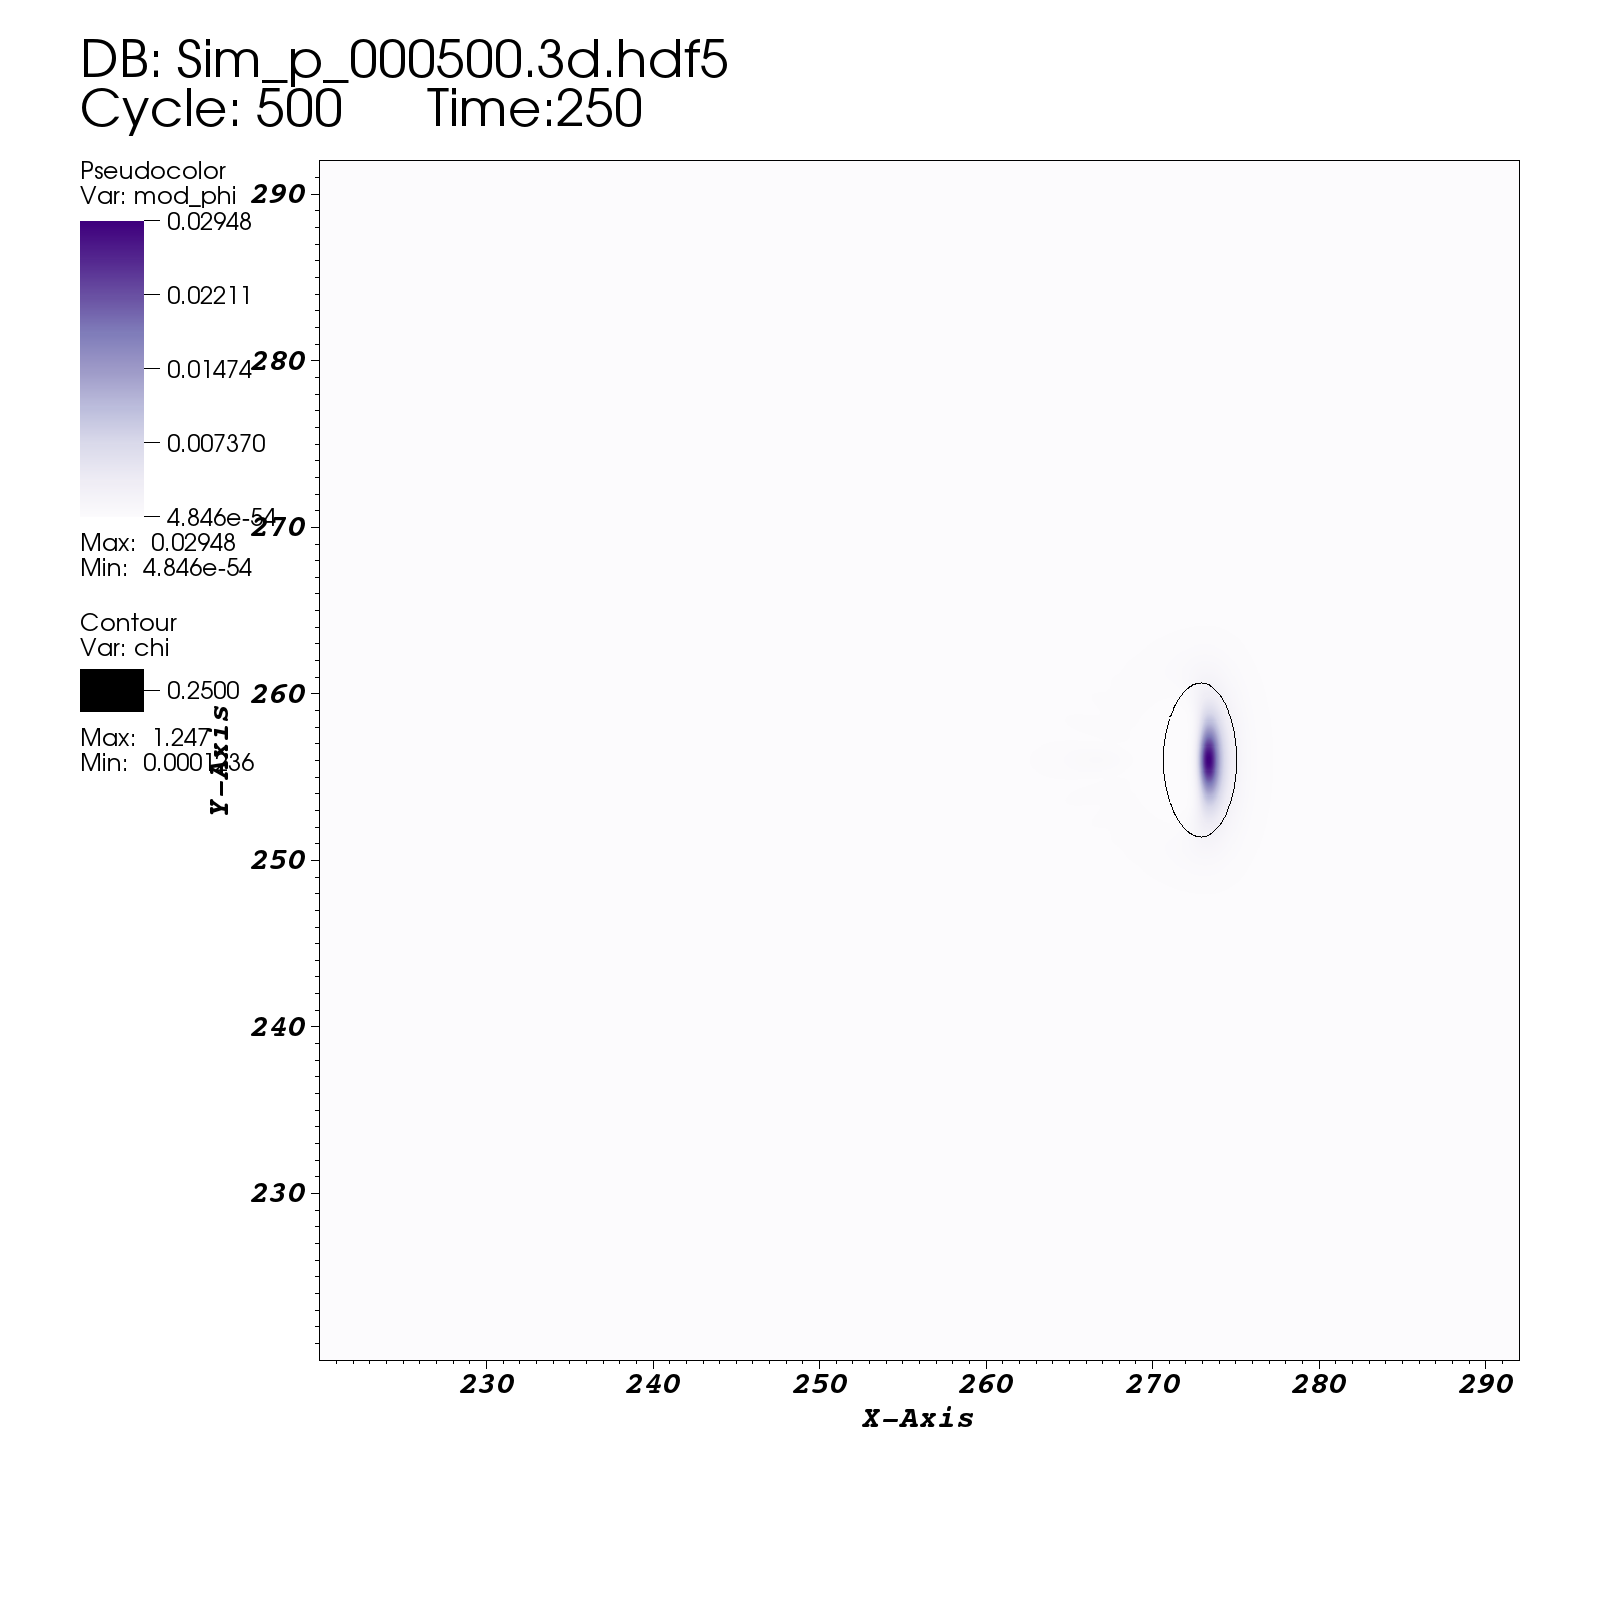
\includegraphics[width=0.45\textwidth]{modphi/headon_bhbs_mod_phi0010.png}}
%   \hfill
%   \subfloat{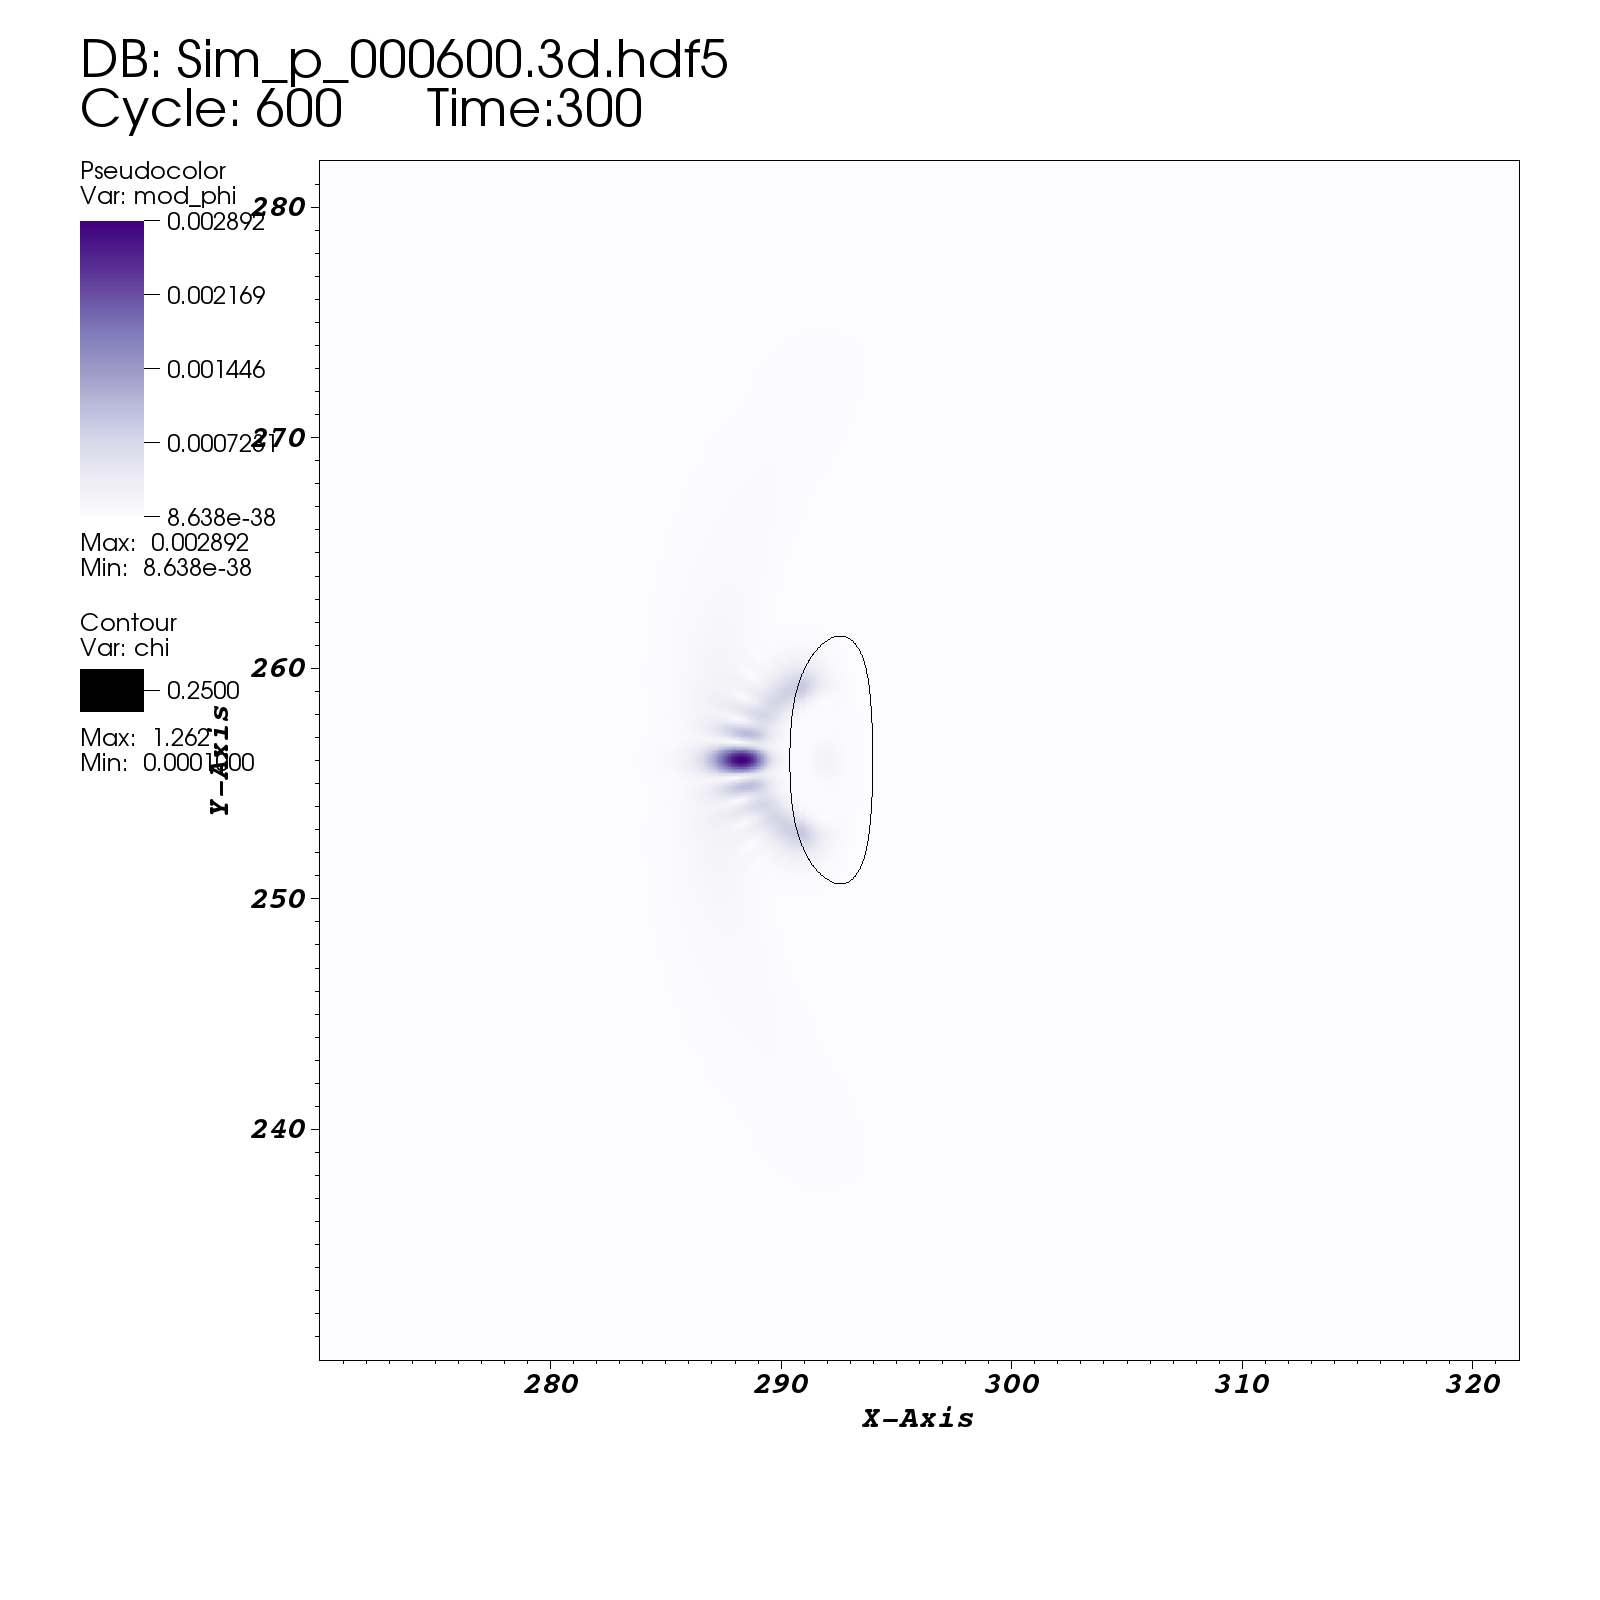
\includegraphics[width=0.45\textwidth]{modphi/headon_bhbs_mod_phi0012.png}}
%   \subfloat{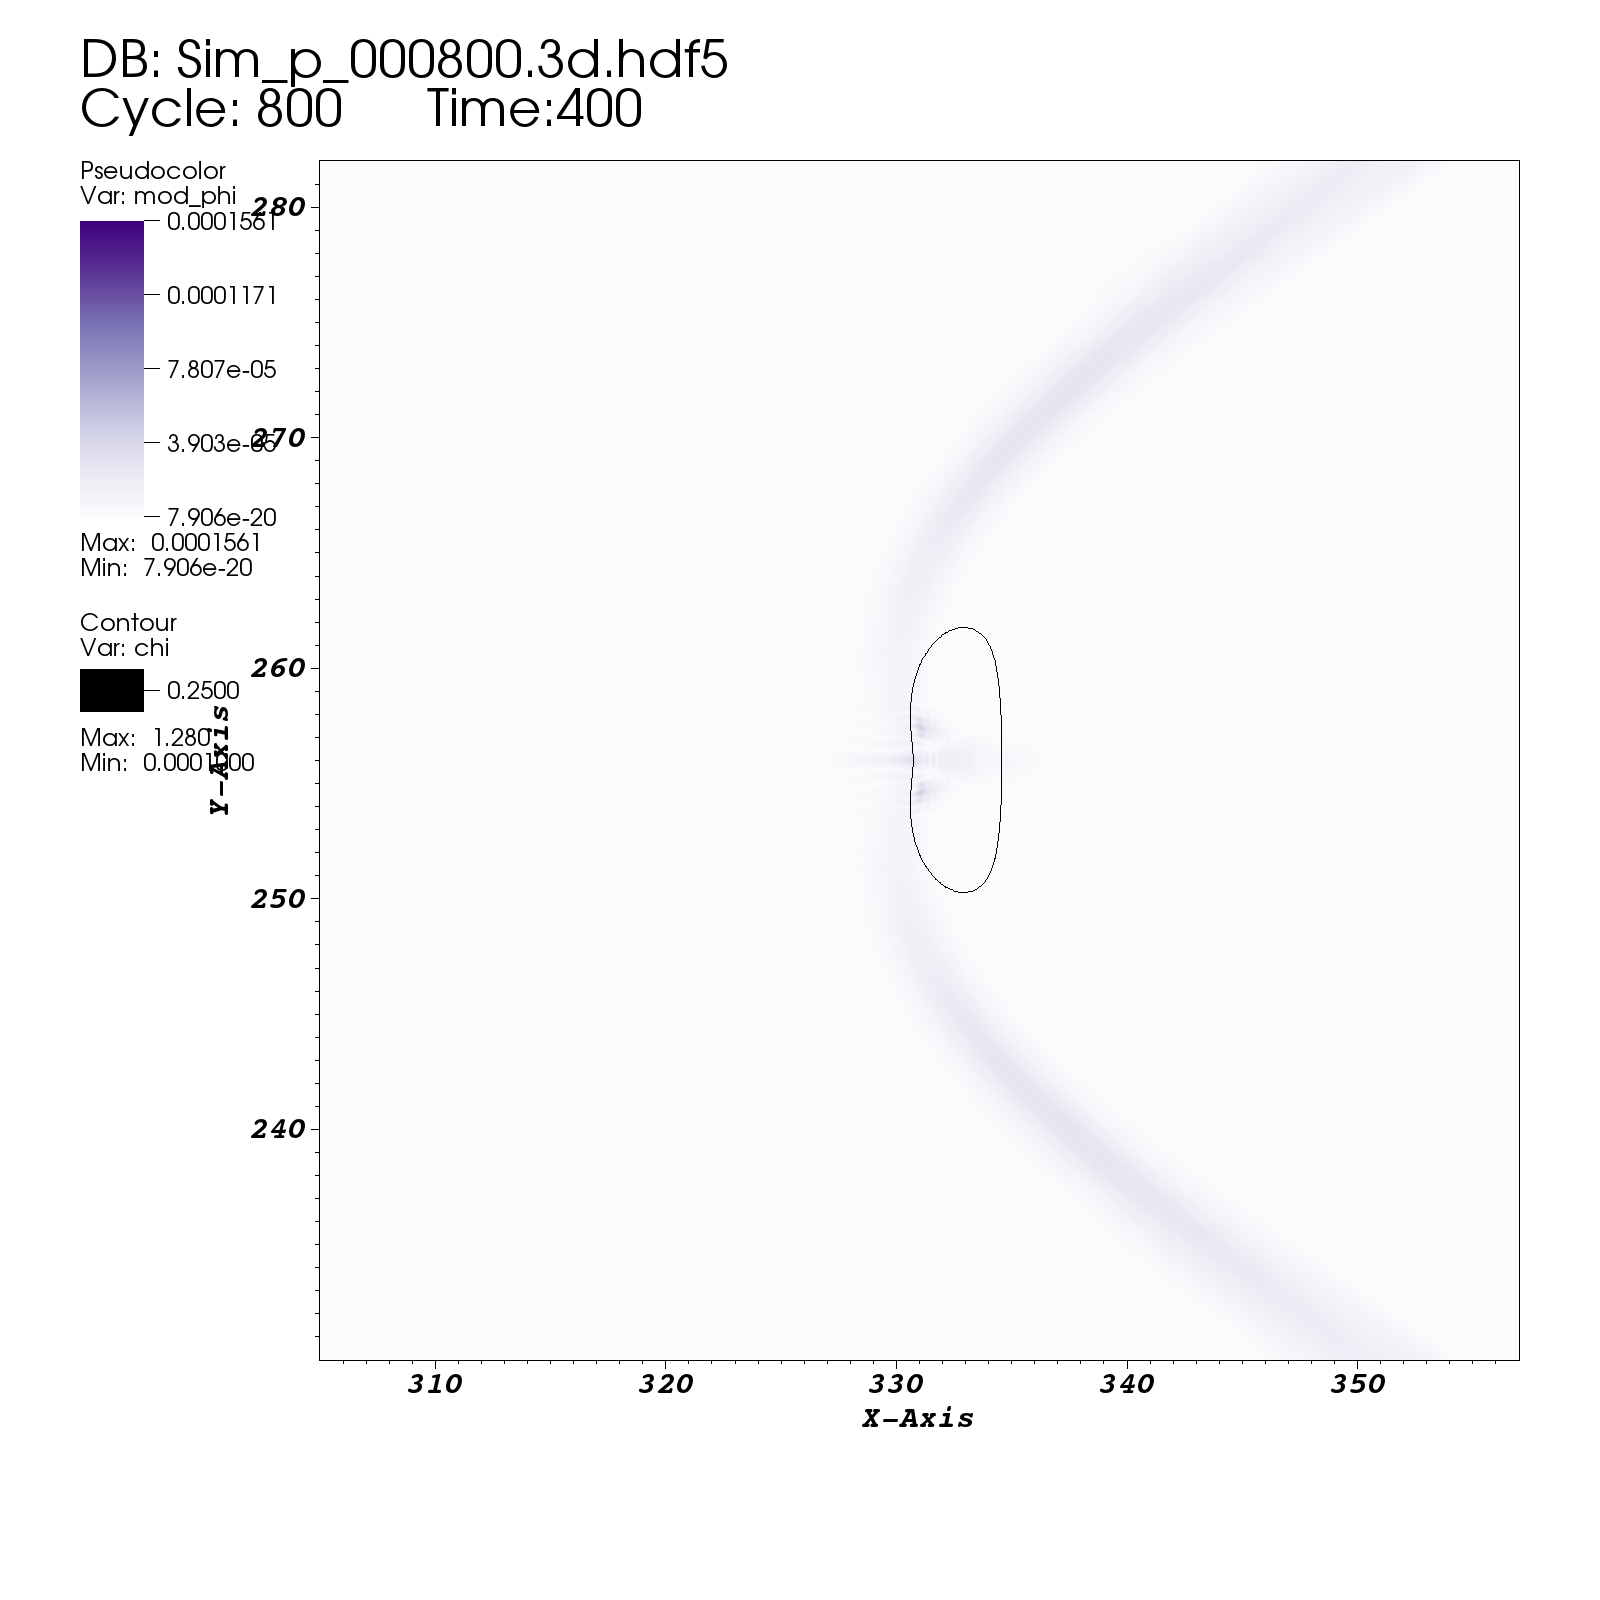
\includegraphics[width=0.45\textwidth]{modphi/headon_bhbs_mod_phi0016.png}}
% \end{figure}




% \subsubsection{Grazing Collision}
%  \begin{figure}[h!]
%   \caption{Left: Maximum of $|\vp|$ during evolution, Right: Total integrated Noether charge $N$.}
%   \centering
%   \subfloat{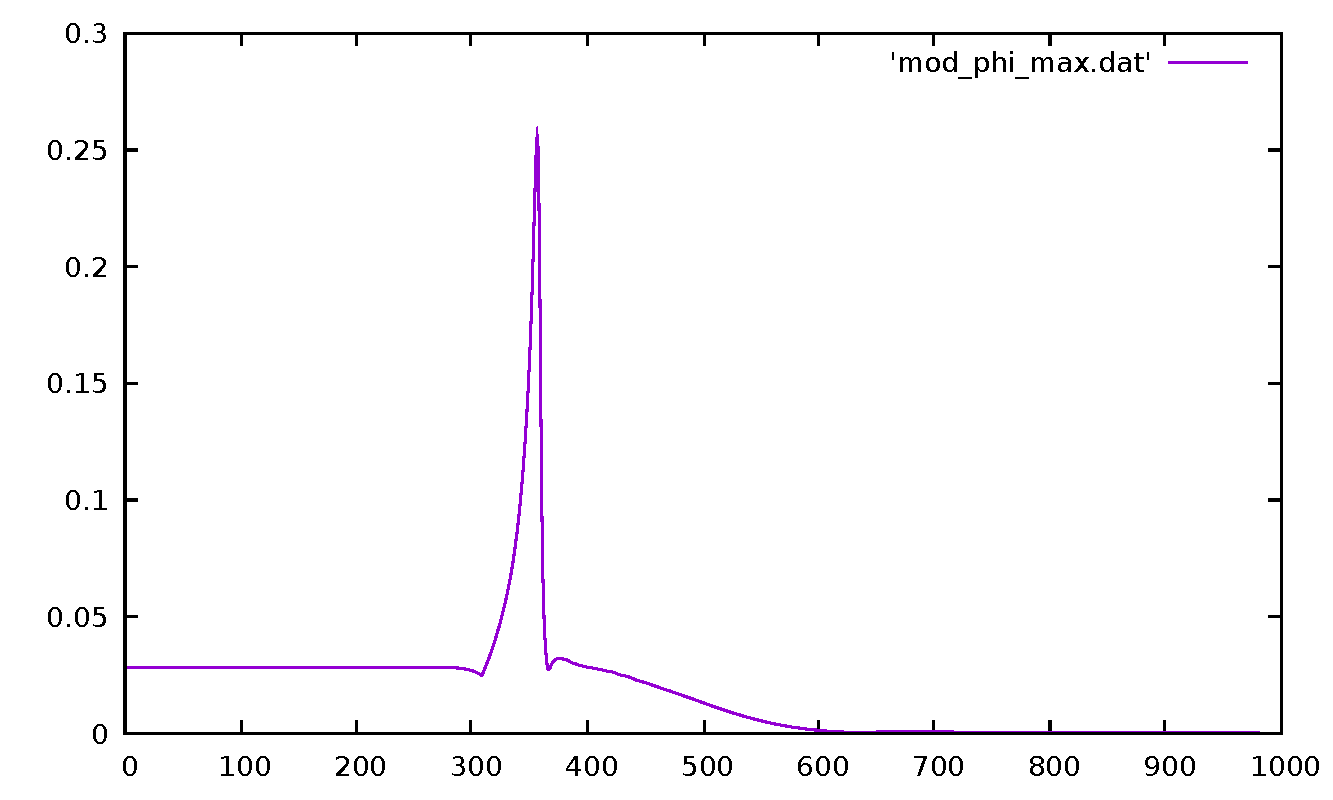
\includegraphics[width=0.5\textwidth]{data/graze_modphi.pdf}\label{boson:fig:f15}}
%   \hfill
%   \subfloat{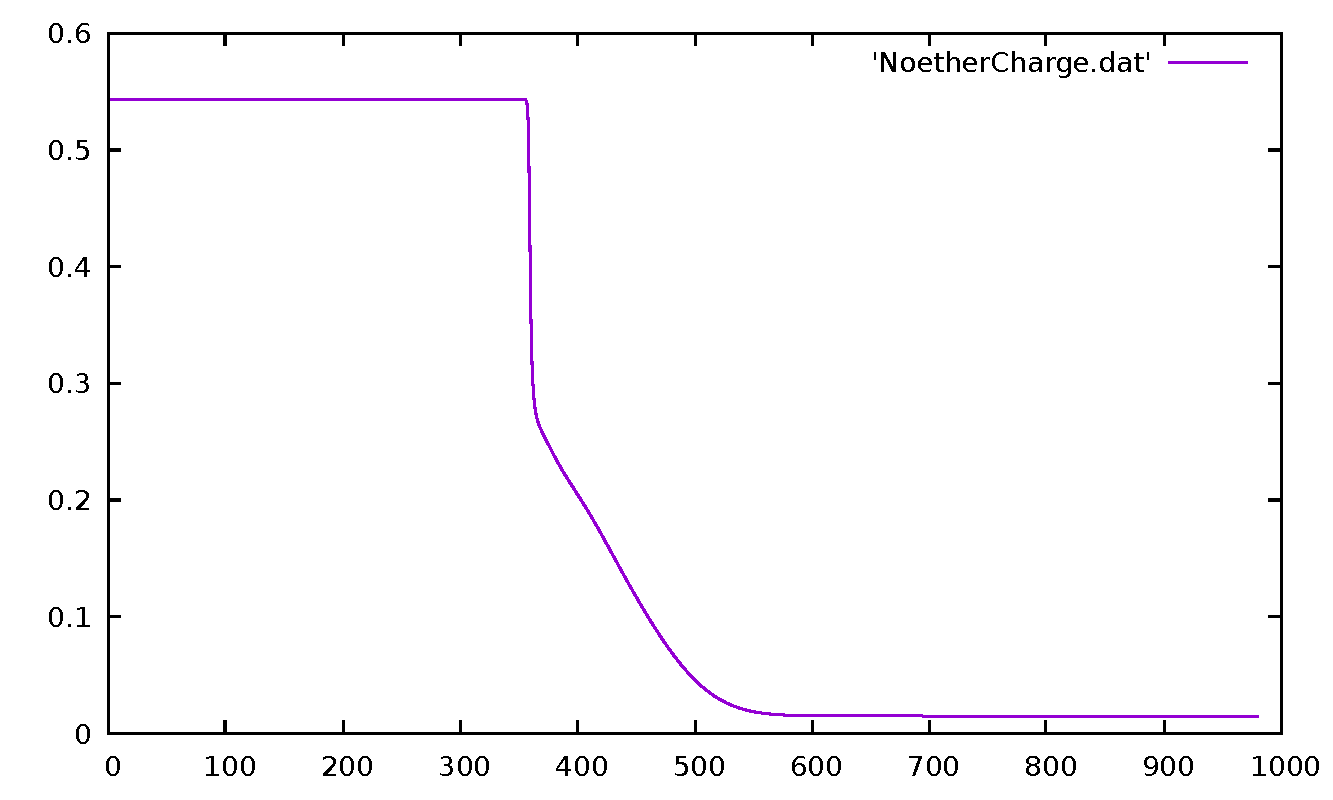
\includegraphics[width=0.5\textwidth]{data/graze_N.pdf}\label{boson:fig:f16}}
% \end{figure}

% Figure (\ref{boson:fig:f7}) shows $|\vp|_{\rm max}$, the global maximum value of $|\vp|$, and the total Noether charge as a function of time for the headon collision. At time $t\approx 289 \cdot m$, $|\vp|_{\rm max}$ rapidly increases; a black hole is then formed. At time $t\approx 327 \cdot m$, $|\vp|_{\rm max}$ there is a temporal maximum in $|\vp|_{\rm max}$ as the resolution limit of the simulation is reached and the scalar field is damped away by the Kreiss-Oliger dissipation mentioned in section \ref{grchombo:sec:grchombo}. This damping can also be seen in the Noether charge plot, at a time of $t \approx 326 \cdot m$, where the total charge that should remain constant falls. The lack of sufficient resolution inside the black hole is not disasterous to the external simulation fortunately; the erorrs accumulated are trapped inside the event horizon.

% The gravitational wave extraction at radius $r=140 \cdot m$ is given in figure \ref{boson:fig:f9}. A spin-weighted spherical harmonic decomposition of the Newman-Penrose scalar $\Psi_4$ [REF] has been done and the $m,l = 2,0$ and $m,l = 2,2$ modes are plotted.


% \begin{figure}[h!]
%   \caption{Left: Maximum of $|\vp|$ during evolution, Right: Total integrated Noether charge $N$.}
%   \centering
%   \subfloat{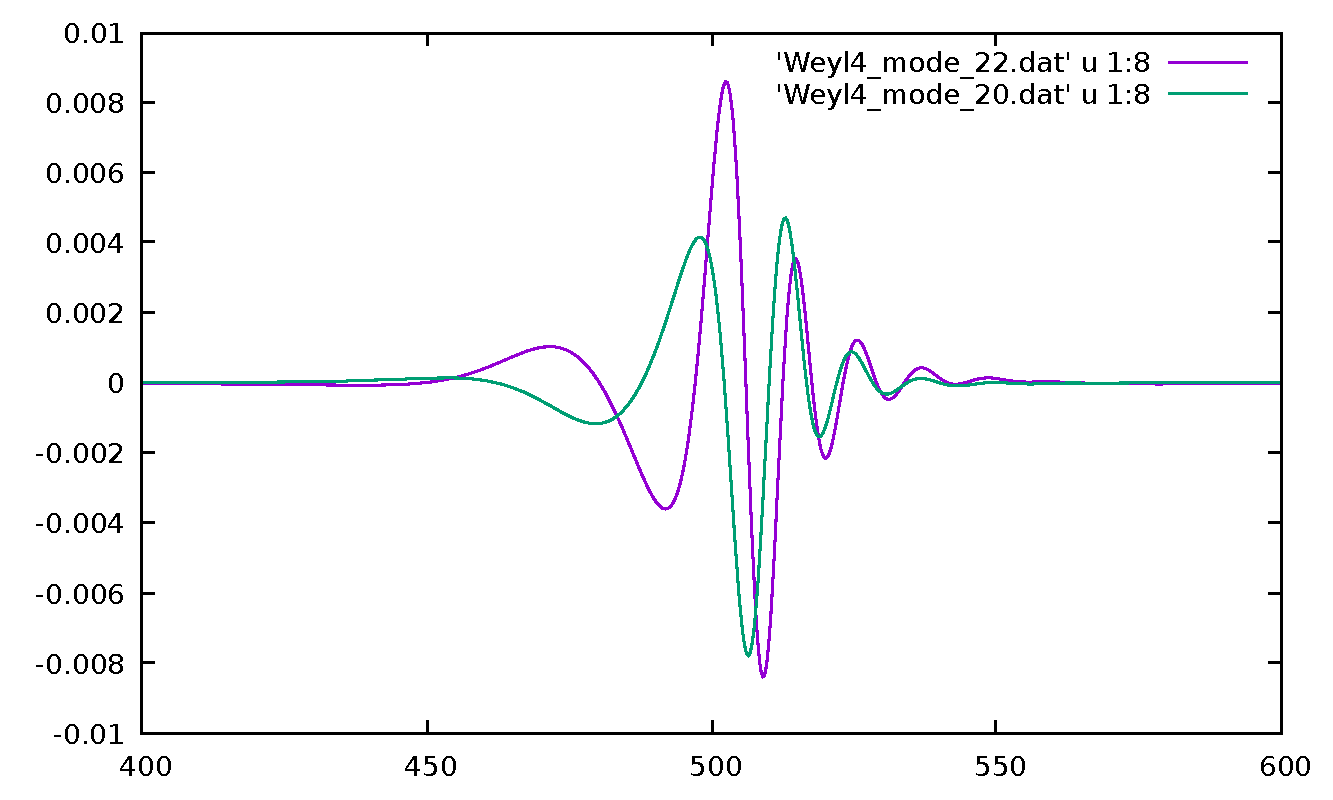
\includegraphics[width=0.5\textwidth]{data/graze_weyl22.pdf}\label{boson:fig:f17}}
% \end{figure}

% The dynamics of the two boson stars are shown in Fig.~(\ref{boson:fig:ff7}) plotting the scalar field modulus $|\vp|$ on the $x,y$ plane. The stars collide at at time $275\cdot m < t < 300 \cdot m$ and soon after an overdensity of scalar field forms collapsing to a black hole. This black hole subsequently accretes the surrouding scalar field; Fig.~(\ref{boson:fig:f7}) shows that the total Noether charge rapidly decays to zero as it falls into the black hole and is dissipated due to finite resolution effects. MAYBE DONT PUT THIS TWICE?



%  \begin{figure}[h!]
%   \caption{Left: Maximum of $|\vp|$ during evolution, Right: Total integrated Noether charge $N$.}
%   \subfloat{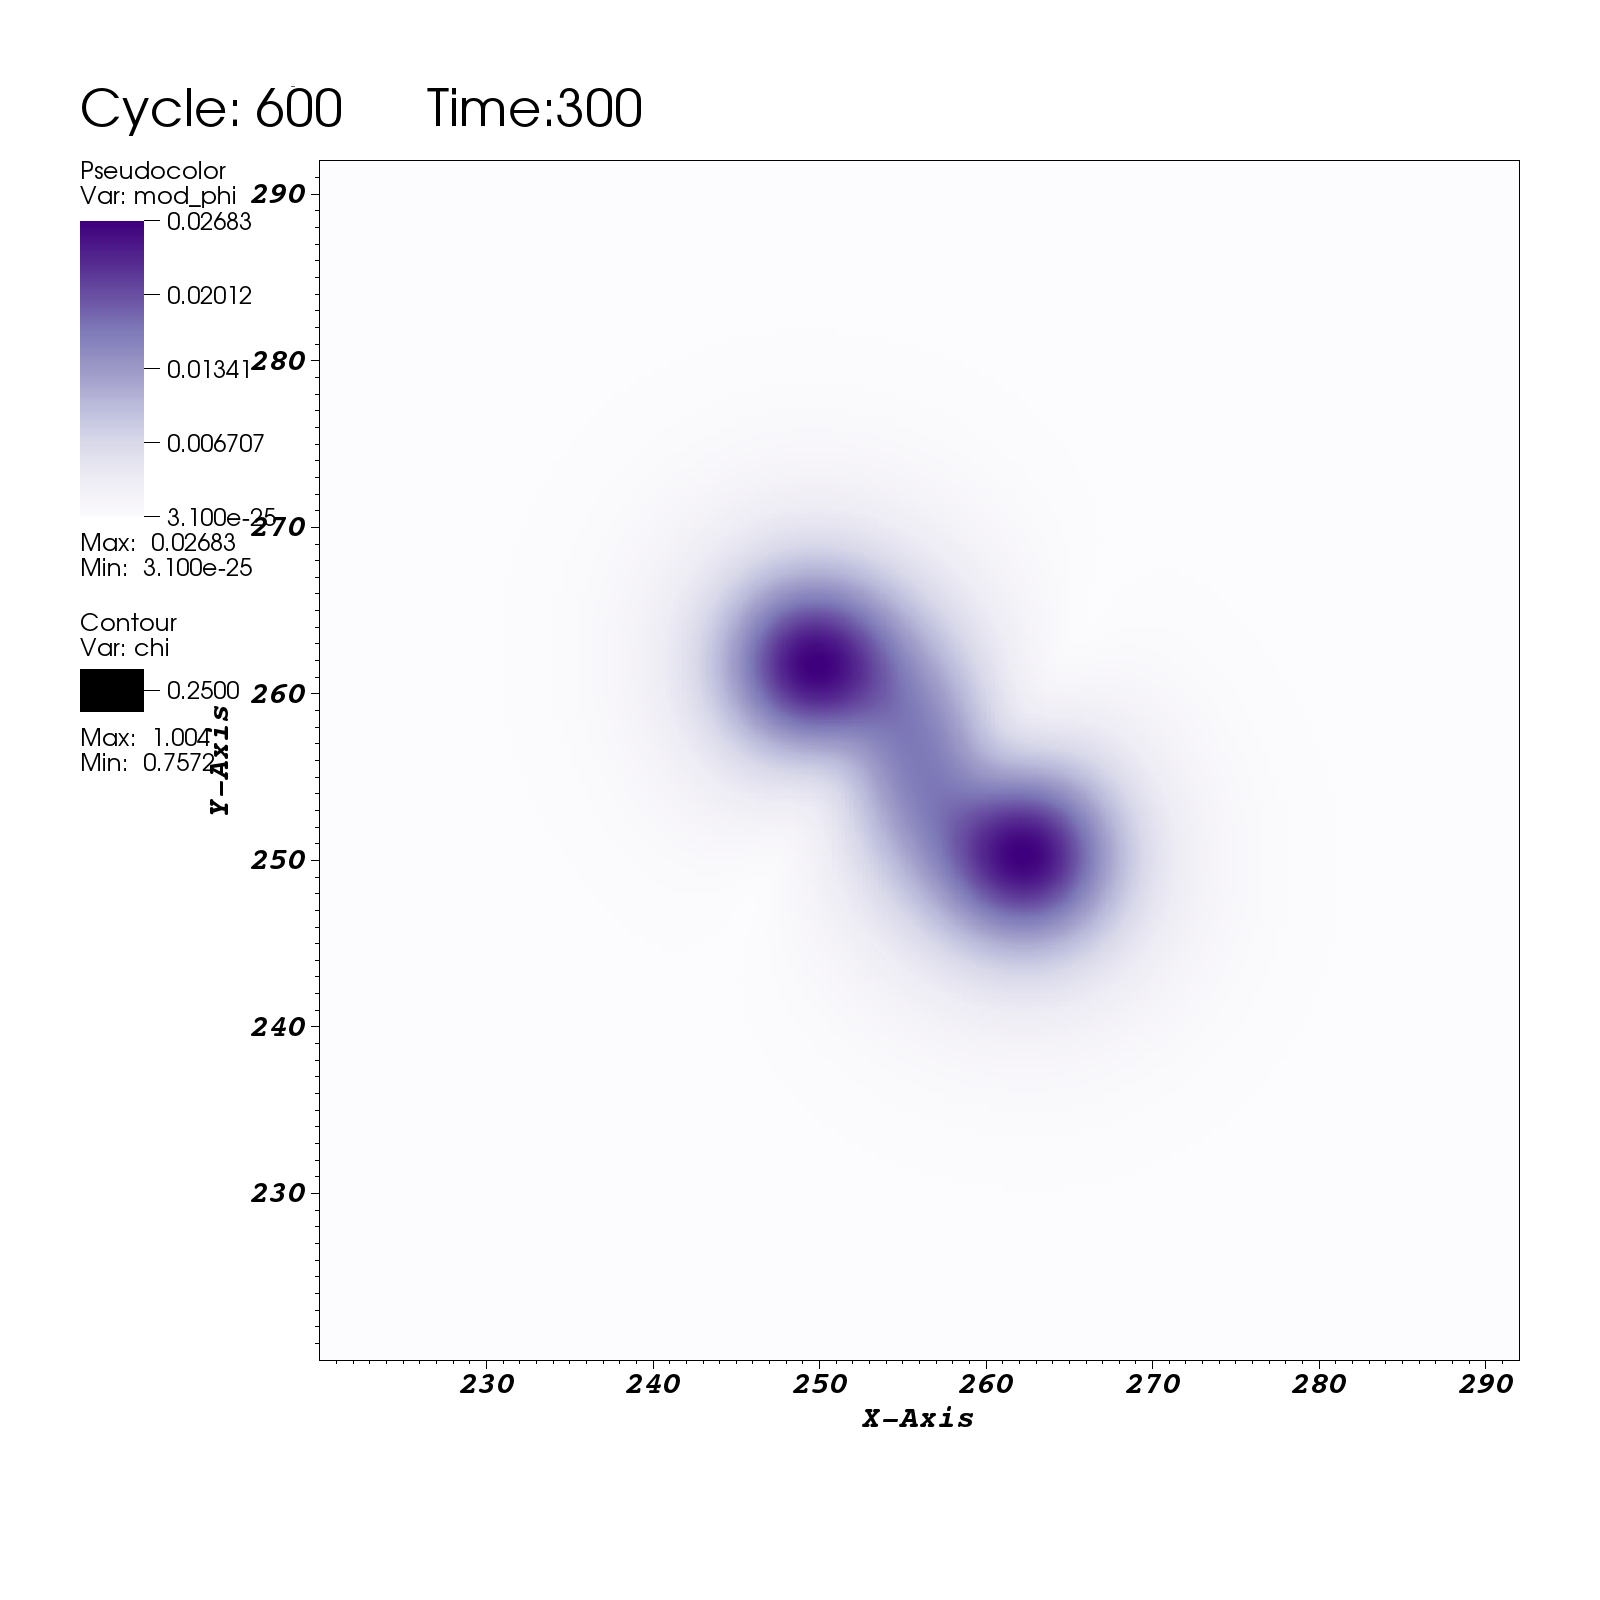
\includegraphics[width=0.45\textwidth]{modphi/graze_mod_phi0012.png}\label{boson:fig:ff15}}
%   \subfloat{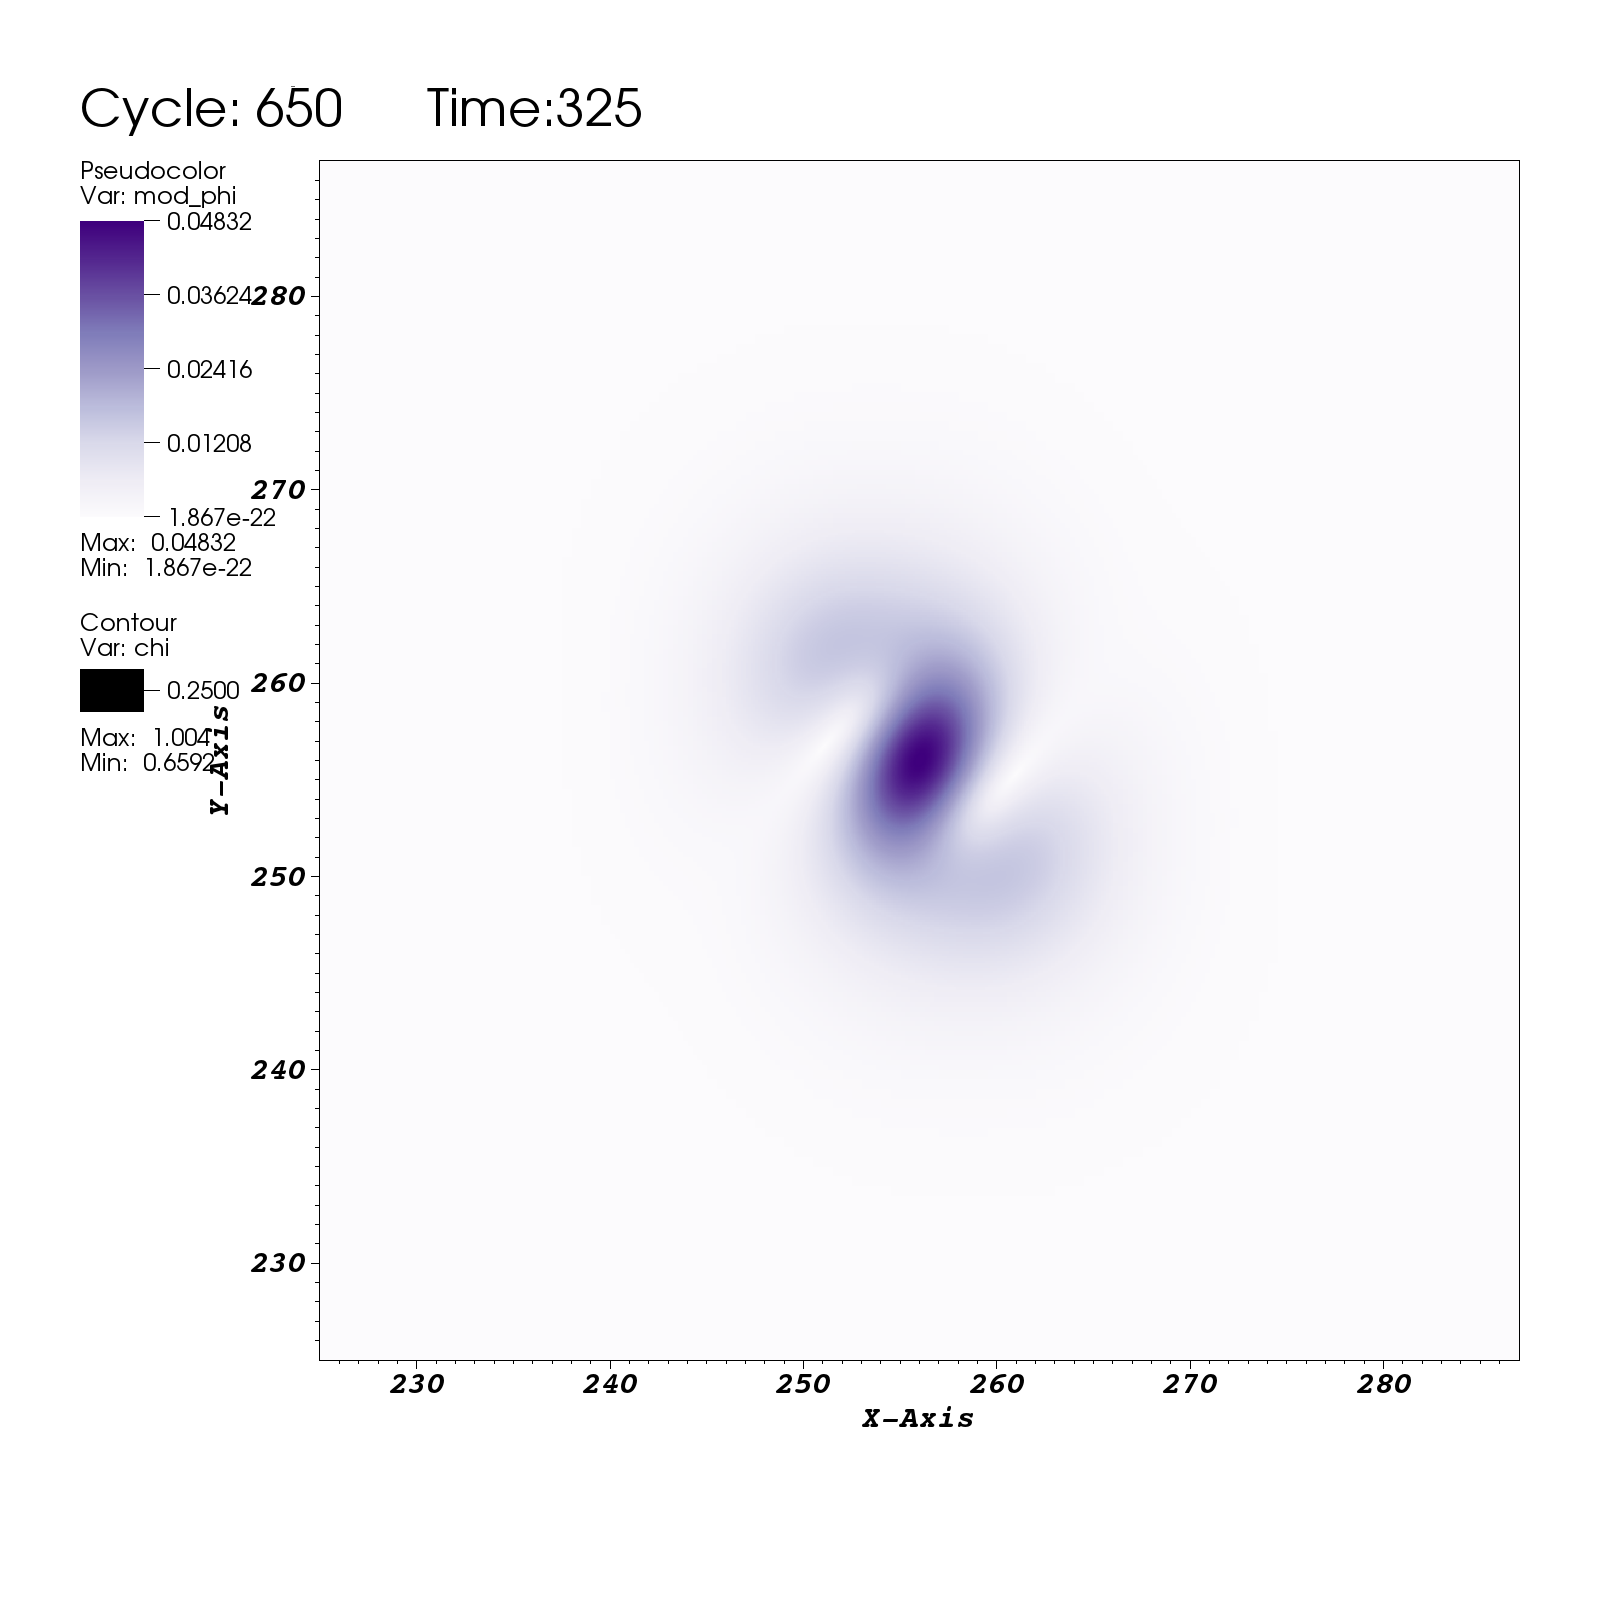
\includegraphics[width=0.45\textwidth]{modphi/graze_mod_phi0013.png}}
%   \hfill
%   \subfloat{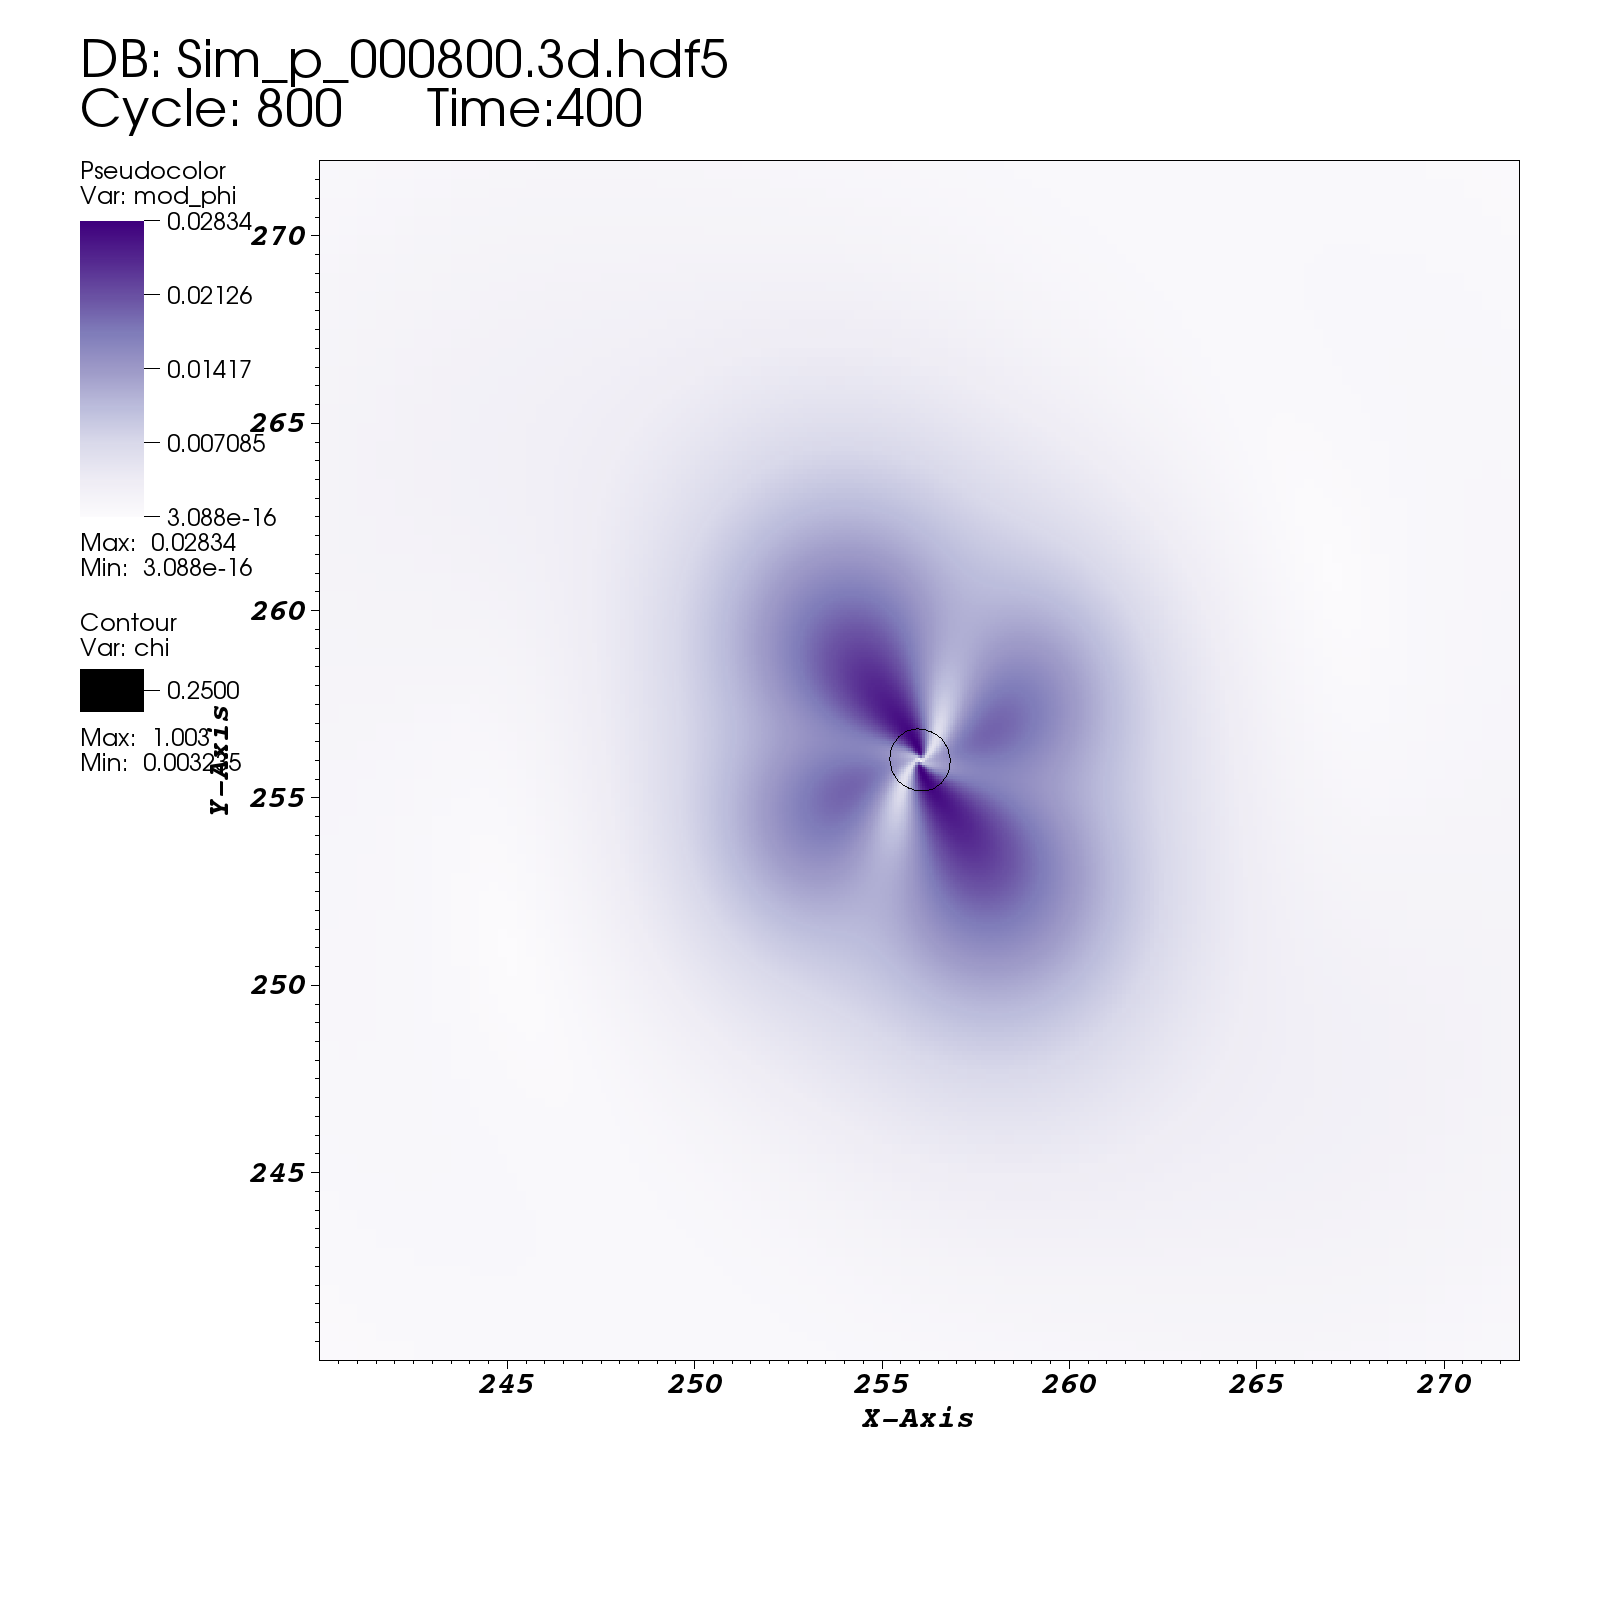
\includegraphics[width=0.45\textwidth]{modphi/graze_mod_phi0016.png}}
%   \subfloat{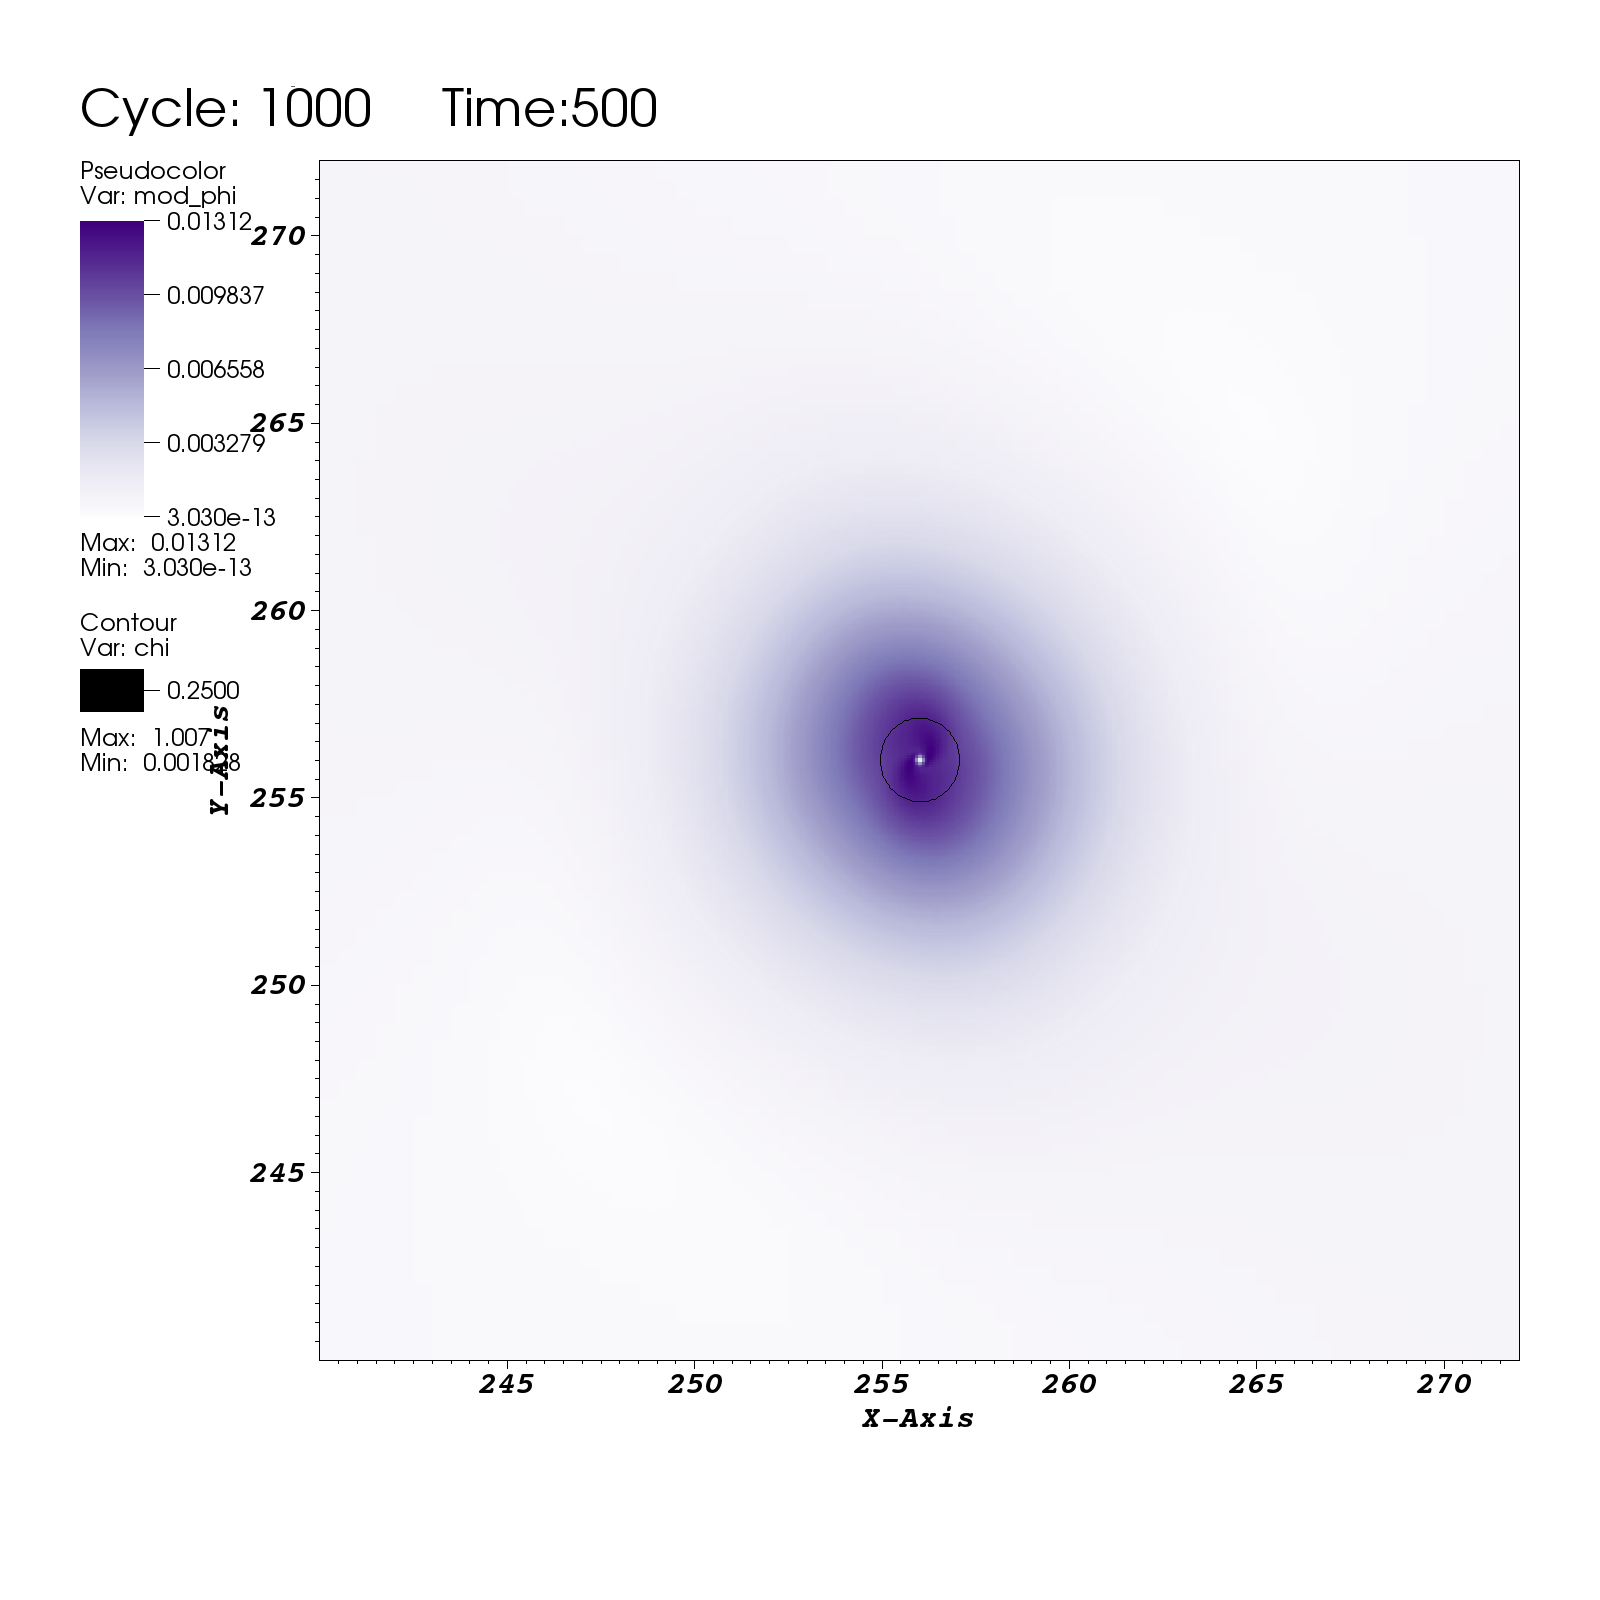
\includegraphics[width=0.45\textwidth]{modphi/graze_mod_phi0020.png}}
% \end{figure}








% THIS WAS ALWAYS UNCOMMENTED, STUFF ABOVE HERE MIGHT BE USEFUL
% THIS WAS ALWAYS UNCOMMENTED, STUFF ABOVE HERE MIGHT BE USEFUL
% THIS WAS ALWAYS UNCOMMENTED, STUFF ABOVE HERE MIGHT BE USEFUL
% THIS WAS ALWAYS UNCOMMENTED, STUFF ABOVE HERE MIGHT BE USEFUL
% THIS WAS ALWAYS UNCOMMENTED, STUFF ABOVE HERE MIGHT BE USEFUL
% THIS WAS ALWAYS UNCOMMENTED, STUFF ABOVE HERE MIGHT BE USEFUL
% THIS WAS ALWAYS UNCOMMENTED, STUFF ABOVE HERE MIGHT BE USEFUL
% THIS WAS ALWAYS UNCOMMENTED, STUFF ABOVE HERE MIGHT BE USEFUL
% THIS WAS ALWAYS UNCOMMENTED, STUFF ABOVE HERE MIGHT BE USEFUL
% THIS WAS ALWAYS UNCOMMENTED, STUFF ABOVE HERE MIGHT BE USEFUL
% THIS WAS ALWAYS UNCOMMENTED, STUFF ABOVE HERE MIGHT BE USEFUL










































% \newpage
% \newpage
% \newpage
% \newpage
% \newpage
% \newpage
% \newpage

% \subsection{After Here is Basically Junk}

% \subsection{Head-on Collisions}
% All the cases studied here are for stationary initial data $\tilde{\A}_{ij}=0,\K=0$ in-falling from an initial separation of $d \cdot m = 32$ due to gravitational attraction. Firstly we consider the equal mass Boson star binary, initial data in figure (). At first they slowly infall creating a short lived object with three maxima, shown in figure (,left), then collapse to a black hole with a decaying spherical harmonic cloud (figures ) outside. As with all the simulations from now on we assume a black hole forms if $\chi \ll 16^{-1}$ where $\chi=16^-1$ is the value taken on the horizon for the isotropic Schwarzschild metric.
%   \begin{figure}[h!]
%   \caption{Initial Data, Left: $\chi$, Right: $|\vp|$.}
%   \centering
%   \subfloat{\includegraphics[width=0.5\textwidth]{headon_bs/chi0000.png}\label{boson:fig:f9}}
%   \hfill
%   \subfloat{\includegraphics[width=0.5\textwidth]{headon_bs/modphi0000.png}\label{boson:fig:f10}}
% \end{figure}
%   \begin{figure}[h!]
%   \caption{Scalar field amplitude before and after black hole formation, Left: Time $t\cdot m = 150$, Right: Time $t \cdot m = 200$.}
%   \centering
%   \subfloat{\includegraphics[width=0.5\textwidth]{headon_bs/modphi0003.png}\label{boson:fig:f11}}
%   \hfill
%   \subfloat{\includegraphics[width=0.5\textwidth]{headon_bs/modphi0004.png}\label{boson:fig:f12}}
% \end{figure}
%    \begin{figure}[h!]
%   \caption{Real part of scalar field after black hole formation, Left: xy plane, Right: yz plane, perpendicular to initial star separation.}
%   \centering
%   \subfloat{\includegraphics[width=0.5\textwidth]{headon_bs/phi_re0004.png}\label{boson:fig:f13}}
%   \hfill
%   \subfloat{\includegraphics[width=0.5\textwidth]{headon_bs/phi_re_perp0004.png}\label{boson:fig:f14}}
% \end{figure}

% The second case considered is the same Boson star outside a black hole parameterised by $M=10M_{BS}$ where $M_{BS}$ is the ADM mass of the Boson star. The scalar field tidally deforms into an ellipsoid with high central density, well beyond Kaup limit of $\vp(0)\sim 0.0764$, and spontaneous collapse to a smaller external black hole is observed. After collapse, figure (), there is an elongated cloud about the new small black hole; there are many nodal lines in $\mathrm{Re}(\vp)$ which focus on the large black hole showing the cloud is in-falling.

%   \begin{figure}[h!]
%   \caption{Initial Data, Left: $\chi$, Right: $|\vp|$.}
%   \centering
%   \subfloat{\includegraphics[width=0.5\textwidth]{LMR/chi0000.png}\label{boson:fig:f15}}
%   \hfill
%   \subfloat{\includegraphics[width=0.5\textwidth]{LMR/modphi0000.png}\label{boson:fig:f16}}
% \end{figure}
%   \begin{figure}[h!]
%   \caption{Final Data at time $t\cdot m = 125$, Left: Conformal factor $\chi$, Right: Scalar field modulus $|\vp|$, Bottom: Real part of scalarfield $\mathrm{Re}(\vp).$}
%   \centering
%   \subfloat{\includegraphics[width=0.5\textwidth]{LMR/chi0005.png}\label{boson:fig:f17}}
%   \hfill
%   \subfloat{\includegraphics[width=0.5\textwidth]{LMR/modphi0005.png}\label{boson:fig:f18}}
%   \\
%    \subfloat{\includegraphics[width=0.5\textwidth]{LMR/phi_re0000.png}\label{boson:fig:f19}}
% \end{figure}
% Final case consists of an equal mass Black Hole and Boson Star, initial configuration in Figure 11. As can be seen from the plot of $\Re(\phi)$ and $|\phi|$, in Figure 12, most of the star falls into the black hole, however some scalar field manages to excite an intricate spherical harmonic cloud pattern.
%   \begin{figure}[h!]
%   \caption{Initial data for equal mass Boson Star and Black Hole, Left: $\chi$, Right: $|\vp|$}
%   \centering
%   \subfloat{\includegraphics[width=0.5\textwidth]{headon/chi0000.png}\label{boson:fig:f20}}
%   \hfill
%   \subfloat{\includegraphics[width=0.5\textwidth]{headon/mod_phi0000.png}\label{boson:fig:f21}}
% \end{figure}
%   \begin{figure}[h!]
%   \caption{Time $t\cdot m=905$ for equal mass Boson Star and Black Hole, Left: $\Re(\vp)$, Right: $|\vp|$}
%   \centering
%   \subfloat{\includegraphics[width=0.5\textwidth]{headon/phi_re0000.png}\label{boson:fig:f22}}
%   \hfill
%   \subfloat{\includegraphics[width=0.5\textwidth]{headon/mod_phi0007.png}\label{boson:fig:f23}}
% \end{figure}

% In all three cases, the Noether charge drops rapidly upon the formation of a black hole; this will be explained in the next section. However some scalar field lingers after collapse, in each case the hair takes the form of spherical harmonics discussed in (). Also observed is the decay of the spherical harmonics to zero amplitude in these simulations with no angular momentum.

% \subsection{Binary Inspiral}
% The only considered case here is the Quasi-circular orbit and inspiral of two equal mass boson stars. The initial boosts were determined by a newtonian calculation yielding
% \begin{equation} v^2 = \frac{M}{2d}\end{equation}
% where $M=0.53(29)$ is the ADM mass of the Boson Star and d is the initial separation. For a relatively low separation of $d\cdot m =32$ code units, shown in Figures 13,14 (Left), we get $v \sim 0.0915$. The boson stars are observed to complete roughly half an orbit before merging and collapse, forming a black hole. Here a Kerr black hole is assumed to have formed as the spacetime has a significant angular momentum which should partially infall with the scalar field.

%   \begin{figure}[h!]
%   \caption{Boson Star $|\vp|$. Left: initial data, Right: later time $t \cdot m = 700$}
%   \centering
%   \subfloat{\includegraphics[width=0.5\textwidth]{inspiral/mod_phi_inspiral_nice0000.png}\label{boson:fig:f24}}
%   \hfill
%   \subfloat{\includegraphics[width=0.5\textwidth]{inspiral/mod_phi_inspiral_nice0002.png}\label{boson:fig:f25}}
% \end{figure}
%   \begin{figure}[h!]
%   \caption{Boson Star $\Re(\vp)$. Left: initial data, Right: later time $t \cdot m = 700$}
%   \centering
%   \subfloat{\includegraphics[width=0.5\textwidth]{inspiral/phi_inspiral_nice0000.png}\label{boson:fig:f26}}
%   \hfill
%   \subfloat{\includegraphics[width=0.5\textwidth]{inspiral/phi_inspiral_nice0002.png}\label{boson:fig:f27}}
% \end{figure}
%   \begin{figure}[h!]
%   \caption{Left: Total Noether charge $\mathcal{N}$ during evolution, Right: $\Psi_4$ over 22 harmonic during evolution.}
%   \centering
%   \subfloat{\includegraphics[width=0.5\textwidth]{inspiral/N.png}\label{boson:fig:f28}}
%   \hfill
%   \subfloat{\includegraphics[width=0.5\textwidth]{inspiral/GW.png}\label{boson:fig:f29}}
% \end{figure}
% Figure 15 shows the total Noether charge, which is no longer conserved. When the black hole forms, the in-falling scalar field moves towards zero radius and gets hugely compressed. The huge compression causes extreme field gradients which induces continuous regridding in the AMR, but this is capped at 7 layers in this simulation to make runtime feasible. When the 8th AMR level is needed it is simply not added and resolution becomes low enough that any Noether charge near the centre is so under-resolved that it seems to fall between the gridpoints. Interestingly, Figures 13,14 (Right) show a scalar field configuration lingering around the black hole, mostly outside the contour $\chi=0.7$, looking like scalar hair. Also Figure 15 (Left) of the Noether charge appears to take significantly longer to decay than in the linear collision simulations. It can be seen in Figure 14 in the plot of $\Re(\vp)$ that the cloud has angular nodes corresponding to angular momentum similarly to boosted stars picking up nodal planes perpendicular to momentum and Figure 10 (Bottom) of the infalling cloud.

% The gravitational wave (GW) signal can be seen in Figure 15 (Right), extracted at a radius $r \cdot m = 90$. At the time $t \cdot m \approx 700$ the gravitational wave signal due to the merger appears; in order to record a longer inspiral simulations with larger initial separations need to be simulated. Currently there appears to be some small problem with the initial data, also observed in the collisions with no angular momentum, that manifests itself in noisy GW extraction and the Hamiltonian constraint initially sharply rising.







%  \chapter{Malaise and Remedy of Binary Boson Star Initial Data}

%  %\documentclass[11pt, book]{report}  %can try book instead  % use "amsart" instead of "article" for AMSLaTeX format
\documentclass[11pt]{report}  %can try book instead   % use "amsart" instead of "article" for AMSLaTeX format
\usepackage[margin = 0.7in, bmargin = 1.1in, tmargin = 0.9in]{geometry}                     % See geometry.pdf to learn the layout options. There are lots.
\geometry{a4paper}                          % ... or a4paper or a5paper or ... 
%\geometry{landscape}                       % Activate for rotated page geometry
\usepackage[parfill]{parskip}           % Activate to begin paragraphs with an empty line rather than an indent
\usepackage{graphicx}               % Use pdf, png, jpg, or eps§ with pdflatex; use eps in DVI mode
                                % TeX will automatically convert eps --> pdf in pdflatex        
\usepackage{amssymb}
\usepackage{amsmath}
\usepackage{amsmath,mathtools}
\usepackage{array}
\usepackage{tabu}
\usepackage{bm}
\usepackage{wrapfig}
\usepackage{multirow}
\usepackage{physics}
\usepackage{hyperref}
\usepackage{listings}
\usepackage[utf8]{inputenc}
\usepackage[T1]{fontenc}
\usepackage{lmodern}
\usepackage{graphicx}
\usepackage{caption}
\usepackage{floatrow}
\usepackage{subfig}
\usepackage{multicol}
\usepackage{xcolor}
\usepackage{pagecolor}
\usepackage{lipsum}  
\usepackage{mdframed}
\usepackage{verbatim}
\usepackage{slashed}
%\usepackage[compat=1.1.0]{tikz-feynman}
%\usepackage{animate}


\newcommand{\G}{\mathcal{G}}
\newcommand{\D}{\mathcal{D}}
\newcommand{\E}{\mathcal{E}}
\renewcommand{\S}{\mathcal{S}}
\newcommand{\M}{\mathcal{M}}
\newcommand{\K}{\mathcal{K}}
\renewcommand{\L}{\mathcal{L}}
\newcommand{\R}{\mathcal{R}}
\renewcommand{\P}{\mathcal{P}}
\newcommand{\vp}{\varphi}
\newcommand{\T}{\mathcal{T}}
\newcommand{\A}{\mathcal{A}}
\newcommand{\bs}{\boldsymbol}
\newcommand{\rspace}{\mathbb{R}}
%\newcommand{\dd}{\mathrm{d}} % is included in physics package??

\newcommand{\mL}{\mathcal{L}} 
\newcommand{\xt}{\tilde{x}}    
\newcommand{\pN}{{}_{\perp}N}
\newcommand{\rmi}{{\rm i}}


\definecolor{purple}{RGB}{38,0,75}
\pagecolor{white}
\color{black}

\renewcommand{\vec}[1]{\boldsymbol{#1}}
\newcommand{\iu}{\mathrm{i}\mkern1mu}
\newcommand{\du}{\mathrm{d}}
\newcommand{\new}[1]{\textcolor{red}{#1}}
\newcommand*{\defeq}{\mathrel{\vcenter{\baselineskip0.5ex \lineskiplimit0pt
                     \hbox{\scriptsize.}\hbox{\scriptsize.}}}%
                     =}
\newcommand*{\invdefeq}{=\mathrel{\vcenter{\baselineskip0.5ex \lineskiplimit0pt
                     \hbox{\scriptsize.}\hbox{\scriptsize.}}}%
                     }

\begin{document}



\begin{abstract}
Through numerical simulations of boson-star head-on collisions,
we explore
the quality of binary initial data obtained from the superposition
of single-star spacetimes. 
Our results demonstrate that evolutions starting from a
plain superposition of individual boosted boson-star spacetimes
are vulnerable to significant unphysical artefacts. These
difficulties can be overcome with a simple modification of the
initial data suggested in \cite{Helfer:2018vtq} for collisions of oscillatons.
%\us{Do we need the remainder of the abstract?}
While we specifically consider massive complex scalar field boson star models up to a 6th-order-polynomial potential, we argue that this vulnerability is universal and present in other kinds of
exotic compact systems and hence needs to be addressed.
%\us{The text is nice, but do we really argue that this is
%a universal problem? I don't think we do...}
%We present numerical simulations of head-on collisions of
%equal-mass, non-spinning boson stars.
%Specifically, we consider two types of boson-star models
%in this analysis, mini boson stars composed of a massive, non-interacting
%complex scalar field, and solitonic boson stars where the scalar field
%obeys a potential also including a fourth and a sixth-order term.
%We cover a wide range of initial separations to identify the suitability
%of different constructions of the binary initial data.
%Our results
%demonstrates that plain superposition of individual boosted boson star
%spacetimes is vulnerable to unphysical artifacts and how these
%difficulties may be overcome with a simple modification of the
%initial data suggested in \cite{Helfer:2018vtq} for collisions of oscillatons.
%We extract as our main diagnostics the gravitational-waves
%radiated in the collisions and the properties of apparent horizons
%if formed.
%\th{We focus very much on Boson Stars, though these ideas might likely show improvements for other compact object? }
%\el{I'll turn the abstract around, and start by saying the main point of linear superposition is bad as soon as we could. At present, the result is only stated more than half way through the abstract and some people doesn't have the patience. maybe something like "We showed in this paper that the oft-used linear superposition ansatz for boosted BS star binaries is vulnerable to unphysical spurious artifacts, which lead significant change in the physical composition of the system. We propose a remedy etc. This is a matter of style of course!}
\end{abstract}

\maketitle

%=============================================================================
\section{Introduction}
\label{sec:intro}

% \rc{Robin adds comments using {\tt \textbackslash rc\{text\}.}}

% \noindent
% \th{Thomas adds comments using {\tt \textbackslash th\{text\}.}}

% \noindent
% \mr{Miren adds comments using {\tt \textbackslash mr\{text\}.}}

% \noindent
% \kc{Katy adds comments using {\tt \textbackslash kc\{text\}.}}

% \noindent
% \el{Eugene adds comments using {\tt \textbackslash el\{text\}.}}

% \noindent
% \us{Uli adds comments using {\tt \textbackslash us\{text\}.}}

The rise of gravitational-wave (GW) physics as an observational field,
marked by the detection of GW150914 \cite{Abbott:2016blz} and followed by about 50 further
compact binary events \cite{LIGOScientific:2018mvr,LIGOScientific:2020ibl}
over the past years, has opened
up unprecedented opportunities to explore gravitational phenomena.
From tests of general relativity
\cite{Berti:2015itd,TheLIGOScientific:2016src,Abbott:2018lct,LIGOScientific:2019fpa,LIGOScientific:2020tif,Moore:2021eok}
to the exploration
of BH populations \cite{Trifiro:2015zda,Belczynski:2017gds,LIGOScientific:2020kqk,Baibhav:2020xdf,Gerosa:2021mno}
or charting the universe with independent
new methods \cite{LIGOScientific:2017adf,LIGOScientific:2019zcs}, GW astronomy offers potential for
revolutionary insight into long-standing open questions;
for a review see \cite{Barack:2018yly}.
Some answers,
such as the association of a soft gamma-ray burst with the neutron star merger GW170817
\cite{TheLIGOScientific:2017qsa,Monitor:2017mdv} have already raised our understanding to new levels.
GW physics furthermore establishes new concrete links to other
fields of research, most notably to particle and high-energy
physics and the exploration of the dark sector of the universe
\cite{Cardoso:2014uka,Barack:2018yly}.
Two important ingredients of this remarkable connection are the
characteristic interaction of fundamental fields with compact
objects through superradiance \cite{Brito:2015oca} and their capacity
to form compact objects through an elaborate balance between
the intrinsically dispersive character of the fields and their
self-gravitation. The latter feature has given rise to the
hypothesis of a distinct class of compact objects as early as the
1950s \cite{Wheeler:1955zz}. In contrast to their well known fermionic counterparts --
stars, white dwarfs or neutron stars -- these compact objects are composed
of bosonic particles or fields and, hence, commonly referred to as
{\em Boson Stars} (BS). GW observations provide the first systematic
approach to search for populations of these objects or to constrain their
abundance. As with all other GW explorations, the success of
this exploration is heavily reliant on the availability of accurate
theoretical predictions for the anticipated GW signals.
%to be expected from these
%compact objects and the binary systems they may form.
This type of
calculation, using numerical relativity techniques
% \mr{Is this book you reviewed now the canonical numerical relativity reference?}
\cite{Baumgarte:2021skc}, is the topic of this work.

The idea of bosonic stars dates back to Wheeler's 1955 study of
gravitational-electromagnetic entities or {\it geons}
\cite{Wheeler:1955zz}.
%Even though these
%configurations do not admit genuinely stationary configurations,
%their scalar analogs, often referred to as oscillatons, admit
%compact configurations with astrophysically long life times
%\cite{Seidel:1991zh,Seidel:1993zk}. By generalizing from real to complex-valued fields,
By generalising from real to complex-valued fundamental fields,
it is even possible to obtain genuinely stationary
solutions to the Einstein-matter equations. First
established for spin 0 or scalar fields
\cite{Feinblum:1968nwc,Kaup:1968zz,Ruffini:1969qy}, this idea has more
recently been extended to spin 1 or vector (aka {\it Proca}
\footnote{Even though the term ``boson star''
generally applies to compact objects formed of any bosonic
fields, it is often used to specifically denote stars made
up of a {\it scalar} field. Stars
composed of vector fields, in contrast, are most commonly
referred to as {\it Proca} stars. Unless specified otherwise,
we shall accordingly assume the term boson star to imply
scalar-field matter.})
fields \cite{Brito:2015pxa}
as well as wider classes of scalar BSs
\cite{Alcubierre:2018ahf,Choptuik:2019zji}.
In the wake of the dramatic progress of numerical
relativity in the simulations of black holes (BHs)
\cite{Pretorius:2005gq,Campanelli:2005dd,Baker:2005vv}
(see \cite{Sperhake:2014wpa} for a review),
the modelling of BSs and binary systems involving BSs has rapidly
gathered pace.

The first BS models computed in the 1960s consisted of a
massive but non-interacting complex scalar field $\varphi$.
This class of stationary BSs,
commonly referred to as {\it mini boson stars}, consists of a 
one parameter family of ground-state
solutions characterised by the central
scalar-field amplitude that reveals a stability structure
analogous to that of Tolman-Oppenheimer-Volkoff
\cite{Tolman:1939jz,Oppenheimer:1939ne} stars:
a stable and an unstable branch of ground-state solutions are
separated by the configuration with maximal mass
\cite{Breit:1983nr,Gleiser:1988ih,Seidel:1990jh}. For each ground-state model,
there furthermore exists a countable hierarchy of
excited states with $n>0$ nodes in the scalar profile
\cite{Lee:1991ax,Jetzer:1991jr,Liddle:1992fmk}. Numerical
evolutions of these excited BSs demonstrate their unstable
character, but also reveal significant variation in the
instability time scales \cite{Balakrishna:1997ej}.

Whereas mini BS models are limited in terms of their maximum
compactness, self-interacting scalar fields
%the addition of self-interaction terms
%of the form $\lambda |\varphi|^4$ or of higher order to the
%scalar potential
can result in significantly more compact stars, even
%above that of 
denser than neutron stars
\cite{Colpi:1986ye,Lee:1986ts,Schunck:1999zu,Hartmann:2012da}. This raises the intriguing
question whether compact BS binaries may reveal themselves
through characteristic GW emission analogous to that from
BHs or NSs \cite{Bustillo:2020syj}. Recent studies
conclude that this may well be within the grasp of
next-generation GW detectors and, in the case of favourable
events, even with advanced LIGO
\cite{Sennett:2017etc,DiGiovanni:2020ror,Toubiana:2020lzd}.

One of the characteristic properties of BSs is
the quantised nature of their spin. The linearised
Einstein equations in the slow-rotation limit lead
to a two-dimensional Poisson equation that does not
admit everywhere regular solutions except for trivial
constants; in consequence BSs cannot rotate perturbatively
\cite{Kobayashi:1994qi}. By relaxing the slow-rotation
approximation, Schunck and Mielke \cite{Schunck:1996he}
computed the first (differentially) rotating BSs
and found that these solutions have an integer
ratio of angular momentum to particle number. The
structure of spinning BS models has been studied extensively
over the years \cite{Ryan:1996nk,Yoshida:1997jq,Yoshida:1997qf,Yoshida:1997nd,Schunck:1999pm,Kleihaus:2005me,Kleihaus:2007vk,Kleihaus:2011sx,Collodel:2017biu}. The quantised nature
of the angular momentum also applies to Proca and
{\it Dirac} (spin $\tfrac{1}{2}$) stars
\cite{Herdeiro:2019mbz}, but numerical studies of the formation
of rotating stars have revealed a striking difference
between the scalar and vector case: while collapsing
scalar fields shed all their angular momentum through an
axisymmetric instability, the collapse of vector fields
results in spinning Proca stars with no indication of an
instability \cite{Sanchis-Gual:2019ljs,DiGiovanni:2020ror}.
This observation is supported by analytic calculations
\cite{Dmitriev:2021utv}, but the instability
may be quenched by self-interaction
terms in the potential function or in the Newtonian limit
\cite{Siemonsen:2020hcg}.
For further reviews of the structure and dynamics of single BSs,
we note the reviews
\cite{Mielke:1997re,Mielke:2000mh,Mundim:2010hi,Liebling:2012fv}.

The first simulations of BS binaries have considered the
head-on collision of configurations with phase differences
between the constituent stars or opposite frequencies
\cite{Palenzuela:2006wp}; see also
\cite{Choptuik:2009ww,Bezares:2017mzk}.
The phase or frequency differences manifest themselves most
pronouncedly in the dynamics and GW emission at late times
around merger. These collisions result in either
a BH, a non-rotating BS or a near-annihilation of the scalar
field in the case of opposite frequencies. BS binaries
with orbital angular momentum generate a GW signal
qualitatively similar to that of BH binaries during the
inspiral phase, but exhibit a much more complex structure around
merger \cite{Palenzuela:2007dm,Palenzuela:2017kcg}.
In agreement with the above mentioned BS formation 
studies, the BS inspirals also seem to avoid the formation
of spinning BSs, although they may settle down into
single nonrotating BSs.

%BS binaries are also the focus of this work.
In spite of the
rapid progress of this field, the computation of GW templates
for BSs still lags considerably behind that of BH binaries,
both in terms of precision and coverage of the parameter space.
Clearly, the presence of the matter fields adds complexity to
this challenge, but also alleviates some of the difficulties
through
the non-singular character of the BS spacetimes. The first main goal
of our study is to highlight the substantial risk of obtaining
spurious physical results due to the use of overly simplistic
initial data constructed by plain superposition of single-BS
spacetimes. Our second main goal is to demonstrate
how an astonishingly
simple modification of the superposition procedure,
first identified by Helfer
{\it et al.}~\cite{Helfer:2018vtq} for oscillatons,
overcomes most of the problems encountered with plain
superposition. We summarise our main findings as follows.
%
\begin{list}{\rm{\bf (\arabic{count})}}{\usecounter{count}
             \labelwidth0.5cm \leftmargin1.0cm \labelsep0.2cm \rightmargin0.0cm
             \parsep0.5ex plus0.2ex minus0.1ex \itemsep0ex plus0.2ex}
  \item An adjustment of the superposition procedure, given 
  by Eq.~(\ref{eq:superposplus}), results in a significant
  reduction of the constraint violations inherent to the initial data;
  see Fig.~\ref{fig:ham}.
  %
  \item In the head-on collision of mini BS binaries with rather low compactness,
  we observe a significant drop of the radiated GW energy with increasing
  distance $d$ if we use plain superposition. This physically unexpected dependence
  on the initial separation levels off only for rather large 
  $d\gtrsim 150\,M$,
  where $M$ denotes the Arnowitt-Deser-Misner (ADM) mass
  \cite{Arnowitt:1962hi}. In contrast, the total radiated energy computed from
  the evolution of our adjusted initial data displays the expected
  behaviour over the entire studied range $75.5\,M\le d\le 176\,M$:
  a very mild increase in the radiated energy with $d$. In the limit of large
  $d \gtrsim 150\,M$, both types of simulations agree within numerical uncertainties;
  see upper panel in Fig.~\ref{fig:erad}.
  %
  \item In collisions of highly compact BSs with solitonic potentials,
  the radiated energy is largely independent of the initial separations
  for both initial data types, but for plain superposition we consistently
  obtain $\sim 10\,\%$ more radiation than for the adjusted initial data;
  see bottom panel in Fig.~\ref{fig:erad}. Furthermore,
  we find plain superposition to result in a slightly faster infall.
  The most dramatic difference, however, is the collapse into individual BHs
  of both BSs well before merger if we use plain superposition. No such collapse
  occurs if we use adjusted initial data. Rather,
  these lead to the expected near-constancy of the central scalar-field amplitude
  of the BSs throughout most of the infall; see Fig.~\ref{fig:soli_ampctr}.
  %
  \item We have verified through evolutions of single boosted BSs that the
  premature collapse into a BH is closely related to the spurious metric
  perturbation (\ref{eq:metricpert}) that arises in the plain superposition
  procedure. Artificially adding the same perturbation to a single BS
  spacetime induces an unphysical collapse of the BS that is in
  qualitative and quantitative agreement with that observed in
  the binary evolution starting with plain superposition;
  see Fig.~\ref{fig:soli_ampctr}.
\end{list}
%

The detailed derivation of these results begins
in Sec.~\ref{sec:formalism} with a review of
the formalism and the computational framework of our
%single BS and binary 
BS simulations. We discuss in more detail
in Sec.~\ref{sec:superposition} the construction of initial
data through plain superposition and our modification of this
method. In Sec.~\ref{sec:results}, we compare the dynamics
of head-on collisions of mini BSs and highly compact solitonic BS
binaries starting from both types of initial data. We note
the substantial differences in the results thus obtained
and argue why we regard the results obtained with our
modification to be correct within numerical uncertainties.
We summarise our findings
and discuss future extensions of this work in
Sec.~\ref{sec:conclusions}.

Throughout this work, we use units where the speed of light and
Planck's constant are set to unity, $c=\hbar=1$. We denote
spacetime indices by Greek letters running from 0 to 3 and
spatial indices by Latin indices running from 1 to 3.

%\us{Need paragraph reviewing the most important work here.
%For now I do bullet points.}
%%
%\begin{itemize}
%  \item Seidel, Suen \cite{Seidel:1990jh,Seidel:1991zh} and Balakrishna et al.
%   \cite{Balakrishna:1997ej}: Single excited BH evolutions;
%   Kaup limit separates stable and unstable branches.
%   \item Balakrishna et al. \cite{Balakrishna:2006ru}: Similar study but
%   with 3+1 evolutions.
%   \item Balakrishna et al. \cite{Balakrishna:2007mr}: Similar study for oscillatons;
%   harder to find gauge, but similar physical behaviour.
%   \item Sanchis-Gual et al. \cite{Sanchis-Gual:2019ljs}: 3D BS and Proca star
%   evolutions. nonaxisymmetric instability for BSs, but not Proca stars.
%   \item Palenzuela et al. \cite{Palenzuela:2006wp}: Head-on BS collisions
%   with different phases or opposite frequencies have very different late-time
%   behaviour and GW output.
%   \item Palenzuela et al. \cite{Palenzuela:2007dm,Palenzuela:2017kcg}: Orbiting
%   BS binaries; inspiral GW signal fiarly simple, but
%   complex behaviour around merger, as it settles down into
%   a nonrotating BS.
%   \item Liebling, Palenzuela \cite{Liebling:2012fv}: LRR.
%   \item Mundim's PhD \cite{Mundim:2010hi}: Numerical BS evolutions; inspiral
%   for up to two orbits (major progress at the time).
%   \item Colpi, Wasserman \cite{Colpi:1986ye}: They found that self-interaction
%   can give much more compact BSs.
%   \item Schunck, Mielke \cite{Schunck:1996he}: First differentially rotating BSs;
%   integer ratio angular momentum to particle number.
%   \item Sennett et al. \cite{Sennett:2017etc}: Estimate how well LIGO and 3G
%   detectors may measure tidal deformation of BSs. Distinction from BH or NS
%   binaries possible for high masses or mass ratios with aLIGO. 3G should
%   distinguish the lot.
%   \item Valdez-Alvaro et al. \cite{ValdezAlvarado:2012xc}:
%   Single stars with fermionic and bosonic fields. Similar structure
%   of stable/unstable branches.
%   \item Yoshida, Eriguchi \cite{Yoshida:1994xi}: QNMs of BSs. Short damping time
%   scale of oscillations compared with fluid stars.
%   \item Kobayashi et al. \cite{Kobayashi:1994qi}: BSs cannot rotate
%   perturbatively. They argue that vortex lines will form for rapid roations (?).
%   \item Gleiser \cite{Gleiser:1988rq}: a $\lambda \varphi^4$ term in the
%   potential can give rise to much denser yet stable stars than mini BSs.
%   \item Gleiser, Watkins \cite{Gleiser:1988ih}: Analytic and numerical
%   proof of the stability threshold at the Kaup limit.
%   \item Bezares et al. \cite{Bezares:2017mzk}: Head-on
%   of BSs and BS-anti-BS binaries. End product is a BS
%   or near annihilation of the BSaBS pair. Orbiting BSs
%   instead form a bar that relaxes into a nonspinning BS.
%   \item Choptuik et al. \cite{Choptuik:2019zji}:
%   multi-oscillating BSs.
%   \item Collodel et al. \cite{Collodel:2017biu}:
%   Analyze excited rotating single-BS models.
%   \item Alcubierre et al. \cite{Alcubierre:2018ahf}:
%   $\ell$ boson stars. \cite{Alcubierre:2019qnh,Alcubierre:2021mvs}: Spherically
%   symmetric evolution of $\ell$ BSs; same stability branches
%   as for normal BSs. \cite{Ontanon:2021hbg}: 3+1 code for
%   computing stationary rotating BSs.
%   \item Sanchis-Gual et al. \cite{Sanchis-Gual:2020mzb}:
%   BSs head-ons can form grav.atoms.
% \end{itemize}
% %



%=============================================================================
\section{Formalism}
\label{sec:formalism}

%=============================================================================
\subsection{Action and covariant field equations}
%
The action for a complex scalar field $\varphi$ minimally coupled to gravity is given by
%
\begin{equation}
S = \int\sqrt{-g}\left\{
  \frac{1}{16\pi G}R - \frac{1}{2}\left[ 
  g^{\mu \nu}\nabla_{\mu}\bar{\varphi}\nabla_{\nu}\varphi
  + V(\varphi)\right] \right\} \du^4 x\,,
  \label{eq:action}
\end{equation}
%
where $g_{\alpha\beta}$ denotes the spacetime metric and $R$ the
Ricci scalar associated with this metric. The characteristics
of the resulting BS models depend on the scalar potential
$V(\varphi)$; in this work, we consider {\it mini boson stars}
and {\it solitonic boson stars}, obtained respectively
for the potential functions
%
\begin{equation}
  V_{\rm min} = \mu^2 |\varphi|^2\,,~~~~~~~~~~
  V_{\rm sol} = \mu^2 |\varphi|^2\left(1-2\frac{|\varphi|^2}{\sigma_0^2}
  \right)^2\,.
  \label{eq:pot}
\end{equation}
%
Here, $\mu$ denotes the mass of the scalar field and $\sigma_0$
describes the self-interaction in the solitonic potential
which can result in highly compact stars
\cite{Lee:1986ts}. Note that $V_{\rm sol}\rightarrow 
V_{\rm min}$ in the limit $\sigma_0\rightarrow \infty$.

Variation of the action (\ref{eq:action}) with respect to the
metric and the scalar field yield the Einstein and matter
evolution equations
%
\begin{eqnarray}
  &&G_{\alpha\beta} = 8\pi G T_{\alpha\beta}
  = 8\pi G\left[
  \partial_{(\alpha}\bar{\varphi}\partial_{\beta)}\varphi
  -\frac{1}{2}g_{\alpha\beta}
  \big(
  g^{\mu\nu}\partial_{\mu}
  \bar{\varphi}\partial_{\nu}\varphi+ V(\varphi)
  \big)
  \right]\,, \label{eq:Einstein} \\
  &&\nabla^{\mu}\nabla_{\mu}\varphi = \varphi V'
  \defeq \varphi \frac{\du}{\du |\varphi|^2}
  V\,.
  \label{eq:Boxvarphi}
\end{eqnarray}
%
Readers who are mainly interested in the results of our work
and/or are familiar with the equations governing BS spacetimes
may proceed directly to Sec.~\ref{sec:superposition}.

%\th{I think the rest of this section should be moved to appendix?}
%\us{The problem with that is that a lot of basic variables are
%defined throughout this part and I don't want to introduce them
%several times. How about the following compromise: We can add
%here a sentence that readers interested in the main results
%can move on to Sec.~3.}
%=============================================================================
\subsection{3+1 formulation}
%
For all simulations performed in this work, we employ the
3+1 spacetime split of ADM \cite{Arnowitt:1962hi} and York \cite{York1979}; see also
\cite{Gourgoulhon:2007ue}. Here, the spacetime metric is
decomposed into the physical 3-metric $\gamma_{ij}$, the
shift vector $\beta^i$ and the lapse function $\alpha$ according to
%
\begin{equation}
  \du s^2 = g_{\alpha\beta}\du x^{\alpha}\du x^{\beta}
  = -\alpha^2 \du t^2 + \gamma_{mn}(\du x^m+\beta^m \du t)
  (\du x^n + \beta^n \du t)\,,
\end{equation}
%
%\mr{The English seems slightly off here as 
%$t=\text{const}$ sounds like it should be singular.}
%\us{Slightly modified. Does that work?}
where the level sets $x^0=t=\mathrm{const}$ represent three-dimensional
spatial hypersurfaces with timelike unit normal $n_{\mu}$.
Defining the extrinsic curvature
%
\begin{equation}
  K_{ij} = -\frac{1}{2\alpha}(\partial_t \gamma_{ij}
  -\beta^m\partial_m \gamma_{ij} -\gamma_{im}\partial_j
  \beta^m-\gamma_{mj}\partial_i \beta^m)\,,
  \label{eq:Kij}
\end{equation}
%
the Einstein equations result in a first-order-in-time
set of differential equations for $\gamma_{ij}$ and $K_{ij}$
that is readily converted into the conformal
Baumgarte-Shapiro-Shibata-Nakamura-Oohara-Kojima (BSSNOK)
formulation
\cite{Baumgarte:1998te,Shibata:1995we,Nakamura:1987zz}.
More specifically, we define
%
\begin{eqnarray}
  &&\chi = \gamma^{-1/3}\,,~~~~
  K=\gamma^{mn}K_{mn}\,,~~~~
  \tilde{\gamma}_{ij}=\chi \gamma_{ij}\,, \nonumber \\
  &&
  \tilde{A}_{ij}=\chi\left(K_{ij}-\frac{1}{3}\gamma_{ij}K\right)\,,~~~~
  \tilde{\Gamma}^i=\tilde{\gamma}^{mn}\tilde{\Gamma}^i_{mn}\,,
\end{eqnarray}
%
where $\gamma=\det \gamma_{ij}$, and $\tilde{\Gamma}^i_{mn}$
are the Christoffel symbols associated with $\tilde{\gamma}_{ij}$.
The Einstein equations are then given by (see for example
Sec.~6 in \cite{Cardoso:2014uka} for more details)
%
\begin{align}
  \partial_t \chi &= \beta^m\partial_m \chi
  + \frac{2}{3}\chi( \alpha K-\partial_m \beta^m)\,,
  \label{eq:chit} \\
  %
  \partial_t \tilde{\gamma}_{ij} &=
  \beta^m\partial_m \tilde{\gamma}_{ij}
  + 2 \tilde{\gamma}_{m(i}\partial_{j)}\beta^m
  - \frac{2}{3}\tilde{\gamma}_{ij}\partial_m \beta^m
  -2\alpha \tilde{A}_{ij}\,, \\
  %
  \partial_t K &=
  \beta^m\partial_m K
  -\chi \tilde{\gamma}^{mn}D_m D_n\alpha
  +\alpha \tilde{A}^{mn}\tilde{A}_{mn}
  +\frac{1}{3}\alpha K^2
  +4\pi G \alpha (S+\rho)\,, \\
  %
  \partial_t \tilde{A}_{ij} &=
  \beta^m\partial_m \tilde{A}_{ij}
  +2\tilde{A}_{m(i}\partial_{j)}\beta^m
  -\frac{2}{3}\tilde{A}_{ij}\partial_m \beta^m
  +\alpha K \tilde{A}_{ij}
  -2\alpha\tilde{A}_{im}\tilde{A}^{m}{}_j
  \nonumber \\
  &~~
  +\chi (\alpha \mathcal{R}_{ij}-D_i D_j \alpha -8\pi G
        \alpha S_{ij})^{\rm TF}\,, \\
  %
  \partial_t \tilde{\Gamma}^i &=
  \beta^m \partial_m \tilde{\Gamma}^i
  +\frac{2}{3}\tilde{\Gamma}^i\partial_m \beta^m
  -\tilde{\Gamma}^m\partial_m \beta^i
  +\tilde{\gamma}^{mn}\partial_m\partial_n \beta^i
  +\frac{1}{3}\tilde{\gamma}^{im}\partial_m\partial_n\beta^n
  \nonumber \\
  &~~~
  -\tilde{A}^{im}\left( 3\alpha \frac{\partial_m \chi}{\chi}
        +2\partial_m \alpha\right)
  +2\alpha\tilde{\Gamma}^i_{mn}\tilde{A}^{mn}
  -\frac{4}{3}\alpha\tilde{\gamma}^{im}\partial_m K
  -16\pi G \frac{\alpha}{\chi}j^i\,,
  \label{eq:Gammait}
\end{align}
%
where `TF' denotes the trace-free part and auxiliary expressions
are given by
%
\begin{align}
  \Gamma^i_{jk} &=
  \tilde{\Gamma}^i_{jk}
  -\frac{1}{2\chi}( \delta^i{}_k\partial_j \chi
        +\delta^i{}_j\partial_k \chi
        -\tilde{\gamma}_{jk}\tilde{\gamma}^{im}\partial_m \chi)
        \,, \nonumber\\
  %
  \mathcal{R}_{ij} &= \tilde{R}_{ij}+ \mathcal{R}^{\chi}_{ij}
  \,, \nonumber\\
  %
  \mathcal{R}^{\chi}_{ij} &=
  \frac{\tilde{\gamma}_{ij}}{2\chi}
  \left[
  \tilde{\gamma}^{mn}\tilde{D}_m\tilde{D}_n \chi
  -\frac{3}{2\chi}\tilde{\gamma}^{mn}\partial_m \chi\,\partial_n \chi
  \right]
  +\frac{1}{2\chi}
  \left(
  \tilde{D}_i \tilde{D}_j \chi
  -\frac{1}{2\chi}\partial_i \chi \,\partial_j \chi
  \right)
  \,, \nonumber\\
  %
  \tilde{R}_{ij} &=
  -\frac{1}{2}\tilde{\gamma}^{mn}\partial_m \partial_n\tilde{\gamma}_{ij}
  +\tilde{\gamma}_{m(i}\partial_{j)}\tilde{\Gamma}^m
  +\tilde{\Gamma}^m\tilde{\Gamma}_{(ij)m}
  +\tilde{\gamma}^{mn}
  \left[
  2\tilde{\Gamma}^k_{m(i}\tilde{\Gamma}_{j)kn}
  +\tilde{\Gamma}^k_{im}\tilde{\Gamma}_{kjn}
  \right]\,,\nonumber\\
  %
  D_i D_j \alpha &=
  \tilde{D}_i \tilde{D}_j \alpha
  + \frac{1}{\chi}\partial_{(i}\chi \partial_{j)}\alpha
  -\frac{1}{2\chi}\tilde{\gamma}_{ij}\tilde{\gamma}^{mn}
        \partial_m \chi \,\partial_n \alpha\,.
\end{align}
%
Here, $\tilde{D}$ and $\tilde{\mathcal{R}}$ denote the covariant
derivative and the Ricci tensor of the conformal metric
$\tilde{\gamma}_{ij}$, respectively.

The matter terms in Eqs.~(\ref{eq:chit})-(\ref{eq:Gammait})
are defined by
%
\begin{equation}
  \rho = T_{\mu\nu}n^{\mu}n^{\nu}\,,~~~
  j_{\alpha} = -\bot^{\nu}{}_{\alpha} T_{\mu\nu} n^{\mu}\,,~~~
  S_{\alpha\beta} = \bot^{\mu}{}_{\alpha} \bot^{\nu}{}_{\beta}
        T_{\mu\nu}\,,~~~
  \bot^{\mu}{}_{\alpha}=\delta^{\mu}{}_{\alpha}+n^{\mu}n_{\alpha}\,.
\end{equation}
%
In adapted coordinates, we only need $\rho$ and
the spatial components $j^i$, $S_{ij}$ which are determined
by the scalar field through Eq.~(\ref{eq:Einstein}),
Defining, in analogy to the extrinsic curvature (\ref{eq:Kij}),
%
\begin{equation}
  \Pi = -\frac{1}{2\alpha}
  (
  \partial_t \varphi - \beta^m \partial_m \varphi
  )
  ~~~~~\Leftrightarrow~~~~~
  \partial_t \varphi = \beta^m\partial_m \varphi-2\alpha \Pi\,,
  \label{eq:Pi}
\end{equation}
%
we obtain
%
\begin{eqnarray}
  \rho &=&
  2\Pi \,\bar{\Pi}
  +\frac{1}{2}\partial^m \bar{\varphi}\,\partial_m\varphi
  +\frac{1}{2}V\,,~~~~~
  S+\rho = 8\bar{\Pi}\,\Pi-V\,, \nonumber \\
  %
  j_i &=&
  \bar{\Pi}\partial_i \varphi
  +\Pi \partial_i \bar{\varphi}\,, \nonumber\\
  %
  S_{ij} &=& \partial_{(i}\bar{\varphi}\partial_{j)}\varphi
  - \frac{1}{2}\gamma_{ij}
  \left(
  \gamma^{mn}\partial_m \bar{\varphi}\,\partial_n \varphi
  -4\bar{\Pi} \,\Pi
  +V
  \right)\,. \label{eqn:projectionofstressenergy}
\end{eqnarray}
%
The evolution of the scalar field according to
Eq.~(\ref{eq:Boxvarphi}) in terms of our 3+1 variables
is given by Eq.~(\ref{eq:Pi}) and
%
\begin{equation}
  \partial_t \Pi =
  \beta^m \partial_m \Pi
  + \alpha
  \left[
  \Pi K
  + \frac{1}{2}V'\varphi
  + \frac{1}{4} \tilde{\gamma}^{mn}
  \left(
  \partial_m \varphi\partial_n\chi
  -2\chi\tilde{D}_m\tilde{D}_n \varphi
  \right)
  \right]
  -\frac{1}{2} \chi\tilde{\gamma}^{mn}\partial_m\varphi
  \partial_n \alpha
  \,,
\end{equation}
%
where $V'=\du V/\du (|\varphi|^2)$

Finally, we evolve the gauge variables $\alpha$ and $\beta^i$
with 1+log slicing and the $\Gamma$-driver condition
(the so-called moving puncture conditions
\cite{Campanelli:2005dd,Baker:2005vv}),
%
%\mr{I thought you use the first order Gamma driver shift condition?}
%\us{I do for Bowen-York BH binaries. But for the boosted isotropics,
%I typically use the 2nd order version.}
\begin{equation}
  \partial_t \alpha = \beta^m \partial_m \alpha
  -2\alpha K
  \,,~~~
  %
  \partial_t \beta^i = \beta^m\partial_m \beta^i
  +\frac{3}{4}B^i
  \,,~~~
  %
  \partial_t B^i = \beta^m \partial_m B^i
  +\partial_t \tilde{\Gamma}^i
  -\eta B^i\,,
\end{equation}
%
%%
%\begin{eqnarray}
%  \partial_t \alpha &=& \beta^m \partial_m \alpha
%  -2\alpha K
%  \,, \nonumber \\
%  %
%  \partial_t \beta^i &=& \beta^m\partial_m \beta^i
%  +\frac{3}{4}B^i
%  \,, \nonumber \\
%  %
%  \partial_t B^i &=& \beta^m \partial_m B^i
%  -\eta B^i\,,
%\end{eqnarray}
%%
where $\eta$ is a constant we typically set to $M\eta\approx 1$
in units of the ADM mass $M$.

Additionally to the evolution equations (\ref{eq:chit})-(\ref{eq:Gammait}),
the Einstein equations also imply four equations that do not contain time
derivatives, the Hamiltonian and momentum constraints
%
\begin{align}
  &\mathcal{H} \defeq \mathcal{R}+K^2-K^{mn}K_{mn} - 16\pi \rho = 0\,,
  \label{eq:ham} \\
  &\mathcal{M}_i\defeq D_i K - D_m K^m{}_i + 8\pi j_i = 0\,.
  \label{eq:mom}
\end{align}
%
While the constraints are preserved under time evolution in the continuum limit,
some level of violations is inevitable due to numerical noise or imperfections
of the initial data. We will return to this point in more detail in
Sec.~\ref{sec:superposition} below.

For the time evolutions discussed in Sec.~\ref{sec:results},
we have implemented the equations of this section in the
{\sc lean} code \cite{Sperhake:2006cy} which is based on the
{\sc cactus} computational toolkit \cite{Allen:1999}. The
equations are integrated in time with the method of lines
using the fourth-order Runge-Kutta scheme with a
Courant factor $1/4$ and fourth-order
spatial discretisation. Mesh refinement is provided by
{\sc carpet} \cite{Schnetter:2003rb} in the form of ``moving
boxes'' and we compute apparent horizons with
{\sc AHFinderDirect} \cite{Thornburg:1995cp,Thornburg:2003sf}.

%=============================================================================
\subsection{Stationary boson stars and initial data}
%
The initial data for our time evolution are based on single stationary
BS solutions in spherical symmetry.
% The computation of these
% single-star models is a well understood problem
% \cite{Mundim:2010hi,Liebling:2012fv}, but we note the more
% recent extensions to a wider range of configurations such as
% multioscillating boson stars \cite{Choptuik:2019zji}
% and $\ell$ boson stars \cite{Alcubierre:2018ahf}.
%In spherical symmetry,
Using spherical polar coordinates,
areal radius and polar slicing, the
line element can be written as
%
\begin{equation}
  \du s^2 =
  -e^{2\Phi} \du t^2
  + \left(1-\frac{2m}{r}\right)^{-1} \du r^2
  + r^2
  (
  \du \theta^2
  + \sin^2\theta \du \phi^2
  )\,.
  \label{eq:ds2sym}
\end{equation}
%
where $\Phi$ and $m$ are functions of $r$ only.
%We will shortly rescale these variables and therefore mark %them by a tilde at this point.
It turns out convenient to express the complex
scalar field in terms of amplitude and frequency,
%
\begin{equation}
  \varphi(t,r) =
  A(r)
  e^{\iu \omega t}\,,~~~~~\omega = \mathrm{const}\in \mathbb{R}\,.
\end{equation}
%
At this point, our configurations are characterised by two
scales, the scalar mass $\mu$ and the gravitational
constant\footnote{Or, equivalently, the Planck mass
$M_{\rm Pl}=\sqrt{\hbar c/G}=1/\sqrt{G}$ for $\hbar=c=1$.} $G$.
In the following, we absorb $\mu$ and $G$ by rescaling all
dimensional variables according to
%
\begin{equation}
  \hat{t}=\mu t\,,~~~
  \hat{r}=\mu r\,,~~~
  \hat{m}=\mu m\,,~~~
  \hat{A}=\sqrt{G} A\,,~~~
  \hat{\omega}=\omega/\mu\,;
  \label{eq:rescaling}
\end{equation}
%
note that $\mu$ has the dimension of a frequency or wave number
and $\sqrt{G}$ is an inverse mass. Using the Planck mass
$M_{\rm Pl}=1/\sqrt{G}=1.221\times10^{19}\,{\rm GeV}$, we
can restore SI units from the dimensionless numerical variables
according to
%
\begin{equation}
  r = \hat{r} \times
  \left(
  \frac{\mu}{1.937\times 10^{-10}\,{\rm eV}}
  \right)^{-1}\,{\rm km}\,,~~~
  %
  \omega = \hat{\omega}\times
  \frac{\mu}{6.582\times 10^{-16}\,{\rm eV}}\,{\rm Hz}
  \,,~~~
  A=\hat{A}\,M_{\rm Pl}\,,
  \nonumber
\end{equation}
%
and likewise for other variables. The rescaled version
of the potential (\ref{eq:pot}) is given by
%
\begin{equation}
  \hat{V}_{\rm min} = \hat{A}^2\,,~~~~~~~~~~
  \hat{V}_{\rm sol} =
  \hat{A}^2
  \left(
  1-2\frac{\hat{A}^2}{\hat{\sigma}_0^2}
  \right)^2~~\text{with}~~\hat{\sigma}_0=\sqrt{G}\sigma_0\,.
  \label{eq:potentials}
\end{equation}
%
In terms of the rescaled variables, the Einstein-Klein-Gordon
equations in spherical symmetry become
%
\begin{align}
  \partial_{\hat{r}}\Phi &=
  \frac{\hat{m}}{\hat{r}(\hat{r}-2\hat{m})}
  +
  2\pi \hat{r}
  \left(
  \hat{\eta}^2
  +\hat{\omega}^2e^{-2\Phi}\hat{A}^2
  -\hat{V}
  \right)\,, \label{eq:Phir} \\
  %
  \partial_{\hat{r}}\hat{m} &=
  2\pi \hat{r}^2
  \left(
  \hat{\eta}^2
  +\hat{\omega}^2e^{-2\Phi}\hat{A}^2
  +\hat{V}
  \right)\,,
  \\
  %
  \partial_{\hat{r}}\hat{A} &=
  \left(
  1-\frac{2\hat{m}}{\hat{r}}
  \right)^{-1/2}
  \hat{\eta}\,, \\
  %
  \partial_{\hat{r}} \hat{\eta} &=
  -2\frac{\hat{\eta}}{\hat{r}}
  -\hat{\eta}\partial_{\hat{r}}\Phi
  +\left(
  1-\frac{2\hat{m}}{\hat{r}}
  \right)^{-1/2}
  (\hat{V}'-\hat{\omega}^2e^{-2\Phi})\hat{A}~~~
  \text{with}~~
  \hat{V}'=\frac{\du \hat{V}}{\du (\hat{A})^2}\,.
  \label{eq:etar}
\end{align}
%
By regularity, we have the following boundary conditions
at the origin $\hat{r}=0$ and at infinity,
%
\begin{equation}
  \hat{A}(0) = \hat{A}_{\rm ctr} \in \mathbb{R}^+\,,~~~~~
  \hat{m}(0) = 0\,,~~~~~
  \hat{\eta}(0) = 0\,,~~~~~
  \Phi(\infty) = 0\,,~~~~~
  \hat{A}(\infty) = 0\,.
\end{equation}
%
This two-point-boundary-value problem has two free
parameters, the central amplitude $\hat{A}_{\rm ctr}$ and the frequency
$\hat{\omega}$. For a given value $\hat{A}_{\rm ctr}$, however, only
a discrete (albeit infinite) number of frequency values
$\hat{\omega}$ will result in models with $\hat{A}(\infty)=0$;
all other frequencies lead to an exponentially divergent scalar
field as $r\rightarrow \infty$. The ``correct'' frequencies
are furthermore ordered by $\hat{\omega}_n<\hat{\omega}_{n+1}$,
where $n\ge 0$ is the number of zero crossings of the scalar
profile $\hat{A}(\hat{r})$; $n=0$ corresponds to the ground state
and $n>0$ to the $n^{\rm th}$ excited state
\cite{Balakrishna:1997ej}.
Finding the frequency for a
regular star for user-specified $\hat{A}_{\rm ctr}$ and $n$ is
the key challenge in computing BS models. We obtain
these solutions through a shooting algorithm, starting with
the integration of
Eqs.~(\ref{eq:Phir})-(\ref{eq:etar}) outwards for
$\hat{A}(0)=\hat{A}_{\rm ctr}$ specified, $\Phi(0)=1$, and our
``initial guess'' $\hat{\omega}=1$. Depending on the number
of zero crossings in this initial-guess model, we repeat
the calculation by increasing or decreasing $\hat{\omega}$
by one order of magnitude until we have obtained an upper and
a lower limit for $\hat{\omega}$. Through iterative bisection,
we then rapidly converge to the correct frequency. Because
we can only determine $\hat{\omega}$ to double precision,
we often find it necessary to capture the scalar field
behaviour at large radius by matching to its asymptotic behaviour
%
\begin{equation}
  \varphi \sim \frac{1}{\hat{r}}
  \exp\left( {-\sqrt{1-\hat{\omega}^2e^{-2\Phi}}}\right)\,,
\end{equation}
%
outside a user-specified radius $\hat{r}_{\rm match}$. Finally,
we can use an additive constant to shift the function $\Phi(\hat{r})$
to match its outer boundary condition. In practice, we impose
this condition in the form of the Schwarzschild relation
$e^{2\Phi}=(1-2\hat{m}/\hat{r})$ at the outer edge of our
grid; in vacuum this is exact even
at finite radius, and we can safely ignore the scalar field
at this point thanks to its exponential falloff.
%
\begin{figure}[b]
    \centering
    \includegraphics[width=250pt]{statBS.eps}
    \caption{One parameter families of mini BSs (black solid) with a
    non-interacting potential $\hat{V}_{\rm min}$ and solitonic BSs (red dashed) with
    potential $\hat{V}_{\rm sol}$ and $\hat{\sigma}_0=0.2$
    as given in Eq.~(\ref{eq:potentials}). In Sec.~\ref{sec:results}
    we simulate head-on collisions of two specific models
    marked by the circles and with parameters listed in
    Table \ref{tab:models}.
    %{\tt fig:statBS}
    }
    \label{fig:statBS}
\end{figure}
%

For a given potential, the solutions computed with this method
form a one-parameter family characterised
by the central scalar field amplitude $\hat{A}_0$. In
Fig.~\ref{fig:statBS} we display two such families for the
potentials (\ref{eq:potentials}) with $\hat{\sigma}_0=0.2$ in the
mass-radius diagram using the areal radius $\hat{r}_{99}$ containing
$99\,\%$ of the BS's total mass. In that figure, we have also marked
by circles two specific models, one mini BS and one solitonic BS,
which we use in the head-on collisions in Sec.~\ref{sec:results} below.
We have chosen these two models to represent one highly compact and
one rather squishy BS; note that both models are located
to the right of the maximal $\hat{M}(\hat{r})$ and, hence, stable stars.
Their parameters and properties are summarised in Table
\ref{tab:models}.
%
\begin{table}
    \centering
    \begin{tabular}{l|cccccc}
    \hline
    Model & $\sqrt{G}A_{\rm ctr}$ & $\sqrt{G}\sigma_0$ & $\mu M_{\rm BS}$ & $\omega/\mu$ & $\mu r_{99}$ & $\max\frac{m(r)}{r}$  \\
    \hline
    mini & 0.0124 & $\infty$ & $0.395$ & $0.971$ & $22.31$ & $0.0249$ \\
    soli & 0.17 & $0.2$ & $0.713$ & $0.439$ & $3.98$ & $0.222$ \\
    \hline
    \end{tabular}
    \caption{Parameters of the two single, spherically symmetric
    ground state BS models employed for our simulations of
    head-on collisions. Up to the rescaling with the scalar mass
    $\mu$, each BS is determined by the central amplitude
    $A_{\rm ctr}$ of the scalar field and the potential parameter
    $\sigma_0$ of Eq.~(\ref{eq:pot}). The mass $M_{\rm BS}$ of the boson star,
    the scalar field frequency $\omega$, the areal radius $r_{99}$ containing
    $99\,\%$ of the total mass $M_{\rm BS}$ and the compactness, defined here
    as the maximal ratio of the mass function to radius, represent
    the main features of the stellar model.}
    \label{tab:models}
\end{table}
%

The formalism discussed so far provides us with BS solutions
in radial gauge and polar slicing. 
In order to reduce the degree of gauge
adjustment in our moving puncture time evolutions, however,
we prefer using conformally flat
BS models in isotropic gauge. In isotropic coordinates, the line
element of a spherically symmetric spacetime has the form
%\mr{Technically there should probably be a $1/\mu^2$ multiplying 
%the RHS. I guess you can can write $\du \hat{s}^2$ on the LHS...}
%\us{I've also been thinking about $d\hat{s}^2$.
%Maybe you are right and we should do that.}
%
\begin{equation}
  \mu^2 \du s^2 = -e^{2\Phi}\du \hat{t}^2+\psi^4 (\du \hat{R}^2 + \hat{R}^2\du \Omega^2)\,,
  \label{eq:ds2iso}
\end{equation}
%
where $\du \Omega^2=\du\theta^2+\sin^2\theta\,\du \phi^2$. Comparing this
with the polar-areal line element (\ref{eq:ds2sym}), we obtain
two conditions,
%
\begin{equation}
  \psi^4 \hat{R}^2 = \hat{r}^2\,,~~~~~~~~
  \psi^4\du \hat{R}^2=
  X^2 \du \hat{r}^2~~~\text{with}~~~
  X=\left(1-\frac{2\hat{m}}{\hat{r}}\right)^{-1/2}\,.
\end{equation}
%
In terms of the new variable $f(\hat{r})=\hat{R}/\hat{r}$, we obtain the differential equation
%
\begin{equation}
  \frac{\du f}{\du \hat{r}} = \frac{f}{\hat{r}}(X-1)\,,
\end{equation}
%
which we integrate outwards by assuming $\hat{R}\propto \hat{r}$ near $\hat{r}=0$. The
integrated solution can be rescaled by a constant factor to ensure that
at large radii -- where the scalar field has dropped to a negligible level --
we recover the Schwarzschild value
$\psi = 1+\frac{\hat{m}}{2\hat{R}}$, in accordance with Birkhoff's theorem.
Bearing in mind that $\psi^4\hat{R}^2=\hat{r}^2$, this directly leads to
the outer boundary condition
%
\begin{equation}
  \hat{R}_{\rm ob} =
  \frac{\hat{r}_{\rm ob}-\hat{m}_{\rm ob}}{2}
  \left[
  1+
  \sqrt{1-\frac{\hat{m}_{\rm ob}^2}{(\hat{r}_{\rm ob}-\hat{m}_{\rm ob})^2}}
  \right]\,,
\end{equation}
%
end, hence, the overall scaling factor applied to the function $\hat{R}(\hat{r})$.

In isotropic coordinates, the resulting spacetime metric is trivially
converted from spherical to Cartesian coordinates $\hat{x}^i=(\hat{x},\hat{y},\hat{z})$ using
$\du \hat{R}^2 + \hat{R}^2\du \Omega^2=\du \hat{x}^2+\du \hat{y}^2+\du \hat{z}^2$, so that
%
\begin{equation}
  \mu^2 \du s^2 = -e^{2\Phi} \du \hat{t}^2 + \psi^4 \delta_{ij}\du \hat{x}^i \,\du \hat{x}^j
  \,.
\end{equation}
%
For convenience, will drop the caret on the rescaled coordinates
and variables from now on and implicitly assume
that they represent dimensionless quantities to be
converted into dimensional form according to
Eq.~(\ref{eq:rescaling}).

%=============================================================================
\subsection{Boosted boson stars}
%
The single BS solutions can be converted into boosted stars through
a straightforward Lorentz transformation. For this purpose, we denote
the star's rest frame by $\mathcal{O}$ with Cartesian
3+1 coordinates $x^{\alpha}=(t,\,x^k)$
and consider a second frame $\tilde{\mathcal{O}}$ with Cartesian 3+1 coordinates
$\tilde{x}^{\tilde{\alpha}}=(\tilde{t},\,\tilde{x}^{\tilde{k}})$
that moves relative to $\mathcal{O}$ with
constant velocity $v^i$. These two frames are related by the transformation
%
\begin{equation}
  \Lambda^{\tilde{\alpha}}{}_{\mu} = \left( \begin{array}{c|c}
        \gamma & -\gamma v_j \\
        \hline
        -\gamma v^i & \delta^i{}_j+(\gamma-1)\frac{v^i v_j}{|\vec{v}|^2}
  \end{array} \right)~~~~\Leftrightarrow~~~~
  \Lambda^{\mu}{}_{\tilde{\alpha}} = \left( \begin{array}{c|c}
        \gamma & \gamma v_j \\
        \hline
        \gamma v^i & \delta^i{}_j+(\gamma-1)\frac{v^i v_j}{|\vec{v}|^2}
  \end{array} \right)
  \,.
  \nonumber%\label{eq:Lorentzgen}
\end{equation}
%
Starting with the isotropic rest-frame metric (\ref{eq:ds2iso})
and the complex scalar field
$\varphi(t,R)=A(R)e^{\iu \omega t + \vartheta_0}$ with $R=\sqrt{\delta_{mn}x^mx^n}$,
we obtain a general boosted model in terms of the 3+1 variables
in Cartesian coordinates $\tilde{x}^{\tilde{k}}$ as follows.
%
\begin{list}{\rm{\bf (\arabic{count})}}{\usecounter{count}
             \labelwidth0.5cm \leftmargin1.0cm \labelsep0.2cm \rightmargin0.0cm
             \parsep0.5ex plus0.2ex minus0.1ex \itemsep0ex plus0.2ex}
  \item A straightforward calculation leads to the first derivatives of the
  metric, its inverse and the scalar field in Cartesian coordinates $x^i$ in the rest frame,
  %
  \begin{eqnarray}
    \partial_t g_{\mu\nu}=\partial_t g^{\mu\nu}=0\,,~~~&&
    \partial_t \varphi_R = -\omega \varphi_I\,,~~~
    \partial_t \varphi_I = \omega \varphi_R\,,
    \nonumber \\[5pt]
    \partial_i g_{00} = -2e^{2\Phi}\frac{\du \Phi}{\du R} \frac{x^i}{R}\,,
    ~~~~~&&
    \partial_i g^{00} = 2e^{-2\Phi} \frac{\du \Phi}{\du R}\frac{x^i}{R}\,,
    \nonumber \\[5pt]
    \partial_i g_{kk} = 4\psi^3 \frac{\du \psi}{\du R} \frac{x^i}{R}\,,
    && \partial_i g^{kk} = -4\psi^{-5} \frac{\du \psi}{\du R}
          \frac{x^i}{R}\,,
    \nonumber \\[5pt]
    \partial_i \varphi_R = \frac{\eta}{f} \cos(\omega t + \phi_0)\,
        \frac{x^i}{R}\,,~~~~&&
  \partial_i \varphi_I = \frac{\eta}{f} \sin(\omega t + \phi_0)\,
        \frac{x^i}{R}\,,
  \end{eqnarray}
  %
  where $\varphi_R$ and $\varphi_I$ are the real and imaginary part of the
  scalar field, and
  %\mr{I feel like I'm being really stupid but can you 
  %explain how you have no derivatives on the RHS below.}
  %\us{Maybe we should discuss, but if I understand your question
  %correctly, the answer is that we use the Einstein equations
  %for the radial derivatives of $\psi$ and $\Phi$.}
  %
  \begin{equation}
    \frac{\du \psi}{\du R} = -\frac{1}{2}
        \frac{X-1}{X} \frac{\psi}{R}\,,~~~~~
        \displaystyle \frac{\du \Phi}{\du R}=
        \frac{X^2-1}{2XR}+\frac{2\pi R}{f^2}X(\eta^2+\omega^2
        e^{-2\Phi}A^2-V)\,.
  \end{equation}
  %
  \item We Lorentz transform the spacetime metric, the scalar field and their
  derivatives to the boosted frame $\tilde{\mathcal{O}}$ according to
  %\mr{Why is there no tilde on the boosted scalar field? Also, I think you're missing a $\partial_\mu$ in the final equation.}
  %\us{I didn't put one on the scalar field since a scalar doesn't change under trafos. You are totally right about the $\partial$; fixed.}
  %
  \begin{gather}
    \tilde{g}_{\tilde{\alpha}\tilde{\beta}}=
      \Lambda^{\mu}{}_{\tilde{\alpha}}\Lambda^{\nu}{}_{\tilde{\beta}}g_{\mu\nu}
      \,,~~~
    \tilde{g}^{\tilde{\alpha}\tilde{\beta}}=
    \Lambda^{\tilde{\alpha}}{}_{\mu}\Lambda^{\tilde{\beta}}{}_{\nu}g^{\mu\nu}
    \,,~~~
    \partial_{\tilde{\gamma}}\tilde{g}_{\tilde{\alpha}\tilde{\beta}}=
    \Lambda^{\lambda}{}_{\tilde{\gamma}}\Lambda^{\mu}{}_{\tilde{\alpha}}
    \Lambda^{\nu}{}_{\tilde{\beta}}\partial_{\lambda}g_{\mu\nu}
    \,, \nonumber\\
     \tilde{\varphi}(\tilde{x}^{\alpha}) = \varphi(x^{\mu})\,,~~~
    \partial_{\tilde{\alpha}}\tilde{\varphi}=
    \Lambda^{\mu}{}_{\tilde{\alpha}} \partial_{\mu}\varphi\,.
  \end{gather}
  %
  \item We construct the 3+1 variables in the boosted frame from these
  quantities according to
  %
  \begin{align}
    &\tilde{\alpha} = \left(-\tilde{g}^{\tilde{0}\tilde{0}}\right)^{-1/2}
    \,,~~~
    \tilde{\beta}_{\tilde{k}}=\tilde{g}_{\tilde{0}\tilde{k}}
    \,,~~~
    \tilde{\gamma}_{\tilde{k}\tilde{l}}=\tilde{g}_{\tilde{k}\tilde{l}}
    \,,~~~
    \tilde{\beta}^{\tilde{k}}=\tilde{\gamma}^{\tilde{k}\tilde{m}}
    \tilde{\beta}_{\tilde{m}}
    \,, \\
    & \tilde{K}_{\tilde{k}\tilde{l}}=
    -\frac{1}{2\tilde{\alpha}}
    \left(
    \partial_{\tilde{t}}\tilde{\gamma}_{\tilde{k}\tilde{l}}
    -\tilde{\beta}^{\tilde{m}}\partial_{\tilde{m}}\tilde{\gamma}_{\tilde{k}\tilde{l}}
    -\tilde{\gamma}_{\tilde{m}\tilde{l}}\partial_{\tilde{k}}\tilde{\beta}^{\tilde{m}}
    -\tilde{\gamma}_{\tilde{k}\tilde{m}}\partial_{\tilde{l}}\tilde{\beta}^{\tilde{m}}
    \right)\,, \nonumber \\
    &\tilde{\Pi} = -\frac{1}{2\tilde{\alpha}}
    \left(
    \partial_{\tilde{t}}\tilde{\varphi}
    - \tilde{\beta}^{\tilde{m}} \partial_{\tilde{m}}\tilde{\varphi}
    \right)\,,
  \end{align}
  %
  with
  %
  \begin{equation}
    \partial_{\tilde{t}}\tilde{\gamma}_{\tilde{k}\tilde{l}}=
    \partial_{\tilde{0}}\tilde{g}_{\tilde{k}\tilde{l}}
    \,,~~~~~
    \tilde{\gamma}_{\tilde{k}\tilde{m}}
    \partial_{\tilde{l}}\tilde{\beta}^{\tilde{m}}
    =
    \partial_{\tilde{l}}\tilde{g}_{\tilde{0}\tilde{k}}
    - \tilde{\beta}^{\tilde{m}}
    \partial_{\tilde{l}}\tilde{g}_{\tilde{k}\tilde{m}}\,.
  \end{equation}
  %
  \item In addition to these expressions, we need to bear in mind the coordinate
  transformation. The computational domain of our time evolution corresponds
  to the boosted frame $\tilde{\mathcal{O}}$. A
  point $\tilde{x}^{\tilde{\alpha}}=(\tilde{t},\,\tilde{x}^{\tilde{k}})$
  in that domain therefore has rest-frame coordinates
  %
  \begin{equation}
     (t,\,x^k) = x^{\mu} = \Lambda^{\mu}{}_{\tilde{\alpha}}\tilde{x}^{\tilde{\alpha}}\,.
  \end{equation}
  %
  It is at $(t,\,x^k)$, where we need to evaluate the rest frame variables
  $\Phi(R)$, $X(R)$, the scalar field $\varphi(t,R)$ and their
  derivatives. In particular, different points on our initial
  hypersurface $\tilde{t}=0$ will in general correspond to different
  times $t$ in the rest frame.
\end{list}
%

%=============================================================================
\section{Boson-star binary initial data}
\label{sec:superposition}
%
%The construction of boson-star binary initial data also forms part of
%our formalism. The details of this construction, however, are the central
%focus of our work and we therefore
The single BS models constructed according to the procedure of the
previous section are exact solutions of the Einstein equations, affected
only by a numerical error that we can control by increasing the resolution,
the size of the computational domain and the degree of precision of the floating
point variable type employed. The construction of binary initial data is
conceptually more challenging due to the non-linear character of the
Einstein equations; the superposition of two individual solutions will,
in general, not constitute a new solution. Instead, such a superposition
incurs some violation of the constraint equations (\ref{eq:ham}),
(\ref{eq:mom}). The purpose of this section is to illustrate
how we can substantially reduce the degree of constraint
violation with a relatively simple adjustment in the
superposition. Before introducing this ``trick'', we first
summarise the superposition as it is commonly used in numerical
simulations.

%=============================================================================
\subsection{Simple superposition of boson stars}
%
\label{sec:superpossimple}
The most common configuration involving more than one BS
is a binary system, and this is the scenario we will
describe here. We note, however, that the method
generalises straightforwardly to any number of stars.
Let us then consider two individual BS solutions
with their centres located at $x^i_{\rm A}$ and $x^i_{\rm B}$,
velocities $v_{\rm A}^i$ and $v_{\rm B}^i$.
The two BS spacetimes are
described by the 3+1 (ADM) variables $\gamma_{ij}^{\rm A}$,
$\alpha_{\rm A}$, $\beta_{\rm A}^i$ and $K_{ij}^{\rm A}$,
the scalar field variables $\varphi_{\rm A}$ and $\Pi_{\rm A}$,
and likewise for star B. We can construct from these
individual solutions an approximation for a binary BS system
via the pointwise superposition
%
\begin{align}
  &\gamma_{ij} =
  \gamma_{ij}^{\rm A}
  +\gamma_{ij}^{\rm B}
  -\delta_{ij}\,,~~~~~~
  K_{ij} = \gamma_{m(i}
  \left[
  K^{\rm A}_{j)n}
  \gamma_{\rm A}^{nm}
  +K^{\rm B}_{j)n}
  \gamma_{\rm B}^{nm}
  \right]\,,
  \nonumber \\
  %&\alpha =
  %\left(
  %\alpha_{\rm A}^{-2}
  %+\alpha_{\rm B}^{-2}
  %\right)^{-1/2}\,,~~~~~
  %%
  %\beta^i=
  %\gamma^{im}
  %(\beta_m^{\rm A}
  %+\beta_m^{\rm B})\,,
  %\nonumber \\[8pt]
  %%
  &\varphi = \varphi_{\rm A} + \varphi_{\rm B}\,,
  \hspace{0.85cm}~~~~~~~~~~
  \Pi = \Pi_{\rm A} + \Pi_{\rm B}\,.
  \label{eq:superpossimple}
\end{align}
%
One could similarly construct a superposition for the lapse
$\alpha$ and shift vector $\beta^i$, but their values do not
affect the physical content of the initial hypersurface.
In our simulations we instead initialise them by
$\alpha=\sqrt{\chi}$ and $\beta^i=0$.

A simple superposition approach along the lines
of Eq.~(\ref{eq:superpossimple}) has been used in
numerous studies of BS as well as BH binaries
including higher-dimensional BHs
\cite{Palenzuela:2006wp,Palenzuela:2007dm,Shibata:2008rq,Okawa:2011fv,Palenzuela:2017kcg,Sperhake:2019oaw}. For BHs and higher-dimensional
spacetimes in particular, this leading-order approximation
has proved remarkably successful and in some limits
a simple superposition is
exact, such as infinite initial separation,
in Brill-Lindquist initial data for non-boosted
\setcounter{footnote}{6}
BHs\footnote{Note that for Brill-Lindquist one superposes the conformal
factor $\psi$ rather than $\psi^4$ as in the
method discussed here.}
\cite{Brill:1963yv}
%\mr{This isn't quite right since the superposition occurs in 
%$\psi$ rather than $\psi^4$? Maybe add a footnote?}
%\us{Yes, I think you are right. Want to have a go?}
or in the superposition of
Aichelburg-Sexl shockwaves \cite{Aichelburg:1970dh}
for head-on collisions of BHs at the speed of light.
It has been noted in Helfer {\em et al.}~\cite{Helfer:2018vtq}, however,
that this simple
construction can result in spurious low-frequency
amplitude modulations in the
time evolution of binary oscillatons (real-scalar-field cousins of BSs); cf.~their Fig.~7. Furthermore, they have proposed a
straightforward remedy that essentially eliminates this spurious
modulation. As we will see in the next section, the repercussions
of the {\it simple superposition} according to Eqs.~(\ref{eq:superpossimple})
can be even more dramatic for BS binaries, but they can
be cured in the same way as in the oscillaton case.
We note in this context that BSs may be more vulnerable
to superposition artefacts near their centres
due to the lack of a horizon and
its potentially protective character in the superposition of
BHs.
%\el{I would also argue that BH spacetimes have the horizons to protect them from the worse of any superposition effects which is focused on the high energy densities in the center.}

The key problem of the construction (\ref{eq:superpossimple})
is the equation for the spatial metric $\gamma_{ij}$. This is best
illustrated by considering the centre $x_{\rm A}^i$ of star A.
In the limit of infinite separation, the metric field of its
companion star B becomes $\gamma_{ij}^{\rm B}\rightarrow \delta_{ij}$.
This is, of course, precisely the contribution we subtract in
the third term on the right-hand-side and all would be well.
In practice, however, the BSs start from initial positions
$x_{\rm A}^i$ and $x_{\rm B}^i$ with finite separation
$d=||x_{\rm A}^i-x_{\rm B}^i||$ and we consequently perturb
the metric at star A's centre by
%
\begin{equation}
  \delta \gamma_{ij} = \gamma_{ij}^{\rm B}(x^i_{\rm A})
  -\delta_{ij}
  \label{eq:metricpert}
\end{equation}
%
away from its equilibrium value $\gamma_{ij}^{\rm A}(x_{\rm A}^i)$.
This metric perturbation can be interpreted as a distortion of
the volume element $\sqrt{\gamma}$
%$=\sqrt{\det\gamma_{ij}}$
at the centre of star A. More specifically, the volume element
at star A's centre is enhanced by $\mathcal{O}(1)\,\%$ for initial
separations $\mathcal{O}(100)\,M$ and likewise for the centre of
star B (by symmetry); see appendix A of Ref.~\cite{Helfer:2018vtq}
for more details.\footnote{Due to the slow decay of this effect $\propto 1/\sqrt{d}$ \cite{Helfer:2018vtq},
a simple cure in terms of using larger $d$ is often not practical.}
%Bearing in mind that the far field of BS B is well approximated by
%the Schwarzschild metric in isotropic coordinates, we can
%estimate the magnitude of this effect as
%$\delta\gamma_{ij}= $
The energy density $\rho$, on the other hand, is barely altered by the
presence of the other star, because of the exponential fall-off of
the scalar field. The leading-order error therefore consists in a
small excess mass that has been added to each BS's central region.
We graphically illustrate this effect in the upper half of
%
\begin{figure}[t]
    \centering
    \includegraphics[width=350pt]{BosonStarTrick.png}
    \caption{
    Graphical illustration of the spurious dynamics that
    may be introduced by the simple superposition
    procedure (\ref{eq:superpossimple}). {\it Upper panel}:
    The spurious
    increase in the volume element mimics a squeezing of the
    stellar core that effects a pulsation of the star or
    may even trigger gravitational collapse to a BH.
    {\it Lower panel}: No such squeezing occurs with the
    adjusted superposition (\ref{eq:superposplus}),
    and the binary evolution starts with approximately
    unperturbed stars.
    }
    \label{fig:Overview}
\end{figure}
%
Fig.~\ref{fig:Overview} together with some of the possible
consequences.
As we will see, this qualitative interpretation is fully borne out
by the phenomenology we observe in the binaries' time evolutions.

Finally, we would like to emphasise that, while evaluating the constraint violations is in general a good rule of thumb to check whether the field configuration is a solution of the system, it does \emph{not} inform one whether it is \emph{the intended} solution; a system with some constraint violation may have drifted closer to a different, unintended solution. In the present case, in addition to the  increased constraint violation, the constructed BS solutions possess significant excitations. Thus, while applying a constraint damping system like conformal Z4
\cite{Bernuzzi:2009ex,Alic:2011gg}
may eventually drive the system to a solution, it may no longer be what was originally intended to be the initial condition of an unexcited BS star.


%=============================================================================
\subsection{Improved superposition}
%
The problem of the simple superposition is encapsulated
by Eq.~(\ref{eq:metricpert}) and the resulting deviation
of the volume elements at the stars' centres away from their
equilibrium values. At the same time, the equation presents us
with a concrete recipe to mitigate this error: we merely need
to replace in the simple superposition (\ref{eq:superpossimple})
the first relation $\gamma_{ij}=\gamma_{ij}^{\rm A}+\gamma_{ij}^B
-\delta_{ij}$ by
%
\begin{equation}
  \boxed{
  \gamma_{ij}=\gamma_{ij}^{\rm A}+\gamma_{ij}^{\rm B}
  -\gamma_{ij}^{\rm B}(x^i_{\rm A})
  =\gamma_{ij}^{\rm A}+\gamma_{ij}^{\rm B}
  -\gamma_{ij}^{\rm A}(x^i_{\rm B})\,.}
  \label{eq:superposplus}
\end{equation}
%
The two expressions on the right-hand side are indeed equal thanks
to the symmetry of our binary: its constituents have equal mass,
no spin and their velocity components satisfy
$v_{\rm A}^i v_{\rm A}^j=v_{\rm B}^i v_{\rm B}^j$ for all
$i,\,j=1,\,2,\,3$ in the centre-of-mass frame.
Equation (\ref{eq:superposplus}) manifestly ensures that at
positions $x_{\rm A}^i$ and $x_{\rm B}^i$ we now recover
the respective star's equilibrium metric and, hence, volume element.
We graphically illustrate this improvement in the bottom panel
of Fig.~\ref{fig:Overview}.

A minor complication arises from the fact that the resulting
spatial metric does not asymptote towards $\delta_{ij}$
as $R\rightarrow \infty$. We accordingly impose
outgoing Sommerfeld boundary conditions on the asymptotic
background metric $2\delta_{ij}-\gamma_{ij}^{\rm A}(x^i_{\rm B})$;
in a set of test runs, however, we find this correction to result
in very small changes well below the simulation's discretisation errors.

Finally, we note that the leading-order correction to the superposition
as written in Eq.~(\ref{eq:superposplus}) does not work for asymmetric
configurations with unequal masses or spins. Generalising the method
to arbitrary binaries requires the subtraction of 
a spatially varying term rather than a constant
$\gamma_{ij}^{\rm B}(x^i_{\rm A})=\gamma_{ij}^{\rm A}(x^i_{\rm B})$
or $\delta_{ij}$. Such a generalisation may consist, for example,
of a weighted sum of the terms $\gamma_{ij}^{\rm A}(x^i_{\rm B})$
and $\gamma_{ij}^{\rm B}(x^i_{\rm A})$. Leaving this
generalisation for future work, we will focus on equal-mass
systems in the remainder of this study and explore
the degree of improvement achieved with
Eq.~(\ref{eq:superposplus}).

%\el{We should also mention that since the effect scales as $\sqrt{r}$, increasing the distance of the initial separation \emph{may} not help as much, and may increase other inaccuracies associated with a long infall evolution. The argument for $\sqrt{r}$ is described in the \cite{Helfer:2018vtq}, i.e. using a Schwarzchild ansatz, the determinant scales like $\sqrt{r}$ for small perturbations.}

%=============================================================================
\section{Models and results}
\label{sec:results}
%
For our analysis of the two types of superposed initial data,
we will now discuss time evolutions of binary BS head-on collisions.
A head-on collision is characterised
by the two individual BS models and three further parameters,
the initial separation in units of the ADM mass,
$d/M$,
%\mr{Worth defining $M$ here?}
%\us{I thought I had defined it, but maybe I didn't. Might be
%worth redefining anyway. Done.}
and the initial velocities $v_{\rm A}$ and
$v_{\rm B}$ of the BSs. We perform all our simulations in the centre-of-mass
frame, so that for equal-mass binaries, $v_{\rm A}=-v_{\rm B}\invdefeq v$.
One additional parameter arises from the type of superposition
used for the initial data construction: we either use the
``plain'' superposition of Eq.~(\ref{eq:superpossimple}) or
the ``adjusted'' method (\ref{eq:superposplus}).

For all our simulations, we
set $v=0.1$; this value
allows us to cover a wide range of initial separations 
without the simulations becoming prohibitively long.
%
\begin{table}[t]
    \centering
    \caption{The four types of BS binary head-on collisions simulated
    in this study. The individual BSs A and B are given either
    by the mini or solitonic model of Table \ref{tab:models},
    and start with initial
    velocity $v$ directed towards each other. The initial data
    is constructed either by plain superposition
    (\ref{eq:superpossimple}) or by adjusting
    the superposed data according to Eq.~(\ref{eq:superposplus}).
    %Appendix A in Ref.~\cite{Helfer:2018vtq}.
    For each type of binary, we perform five collisions with
    initial separations $d$ listed in the final column.
    %\us{For my own use: The convergence sequences are
    %{\tt mBShod080\_h,~~tmBShod080\_h,~~lsBShod16\_h,~~tlsBShod%16\_h.}}
    }
    \begin{tabular}{r|ccccc}
    \hline
    Label & star A & star B & $v$ & initial data & $d/M$ \\
    \hline
    {\tt mini} & mini & mini & $0.1$ & plain &
    75.5,~101,~126,~151,~176 \\
    {\tt +mini}& mini & mini & $0.1$ & adjusted &
    75.5,~101,~126,~151,~176 \\
    {\tt soli} & soli & soli & $0.1$ & plain &
    16.7,~22.3,~27.9,~33.5,~39.1 \\
    {\tt +soli} & soli & soli & $0.1$ &
    adjusted &
    16.7,~22.3,~27.9,~33.5,~39.1 \\
    \hline
    \end{tabular}
    \label{tab:hods}
\end{table}
%
The BS binary configurations
summarised in Table \ref{tab:hods} then result
in four sequences of head-on collisions labelled
{\tt mini}, {\tt +mini}, {\tt soli} and {\tt +soli},
depending in the nature of the constituent BSs and
the superposition method. For each sequence, we vary the
BSs initial separation $d$ to estimate the dependence of the
outcome on $d$. First, however, we test our interpretation
of the improved superposition (\ref{eq:superposplus})
by computing the level of constraint violations in the
initial data.
%%
%\begin{table}[ht]
%    \centering
%    \begin{tabular}{r|ccccc}
%    \hline
%    Label & BS 1 & BS 2 & $v$ & initial data & initial grid \\
%    \hline
%    {\tt mini} & mini & mini & $0.1$ & plain &
%    $\{(645,322,161)\times(40,20,10),\,h\}$ \\
%    {\tt +mini}& mini & mini & $0.1$ & adjusted &
%    $\{(645,322,161)\times(40,20,10)$,\,h\} \\
%    {\tt soli} & soli & soli & $0.1$ & plain &
%    $\{(357,179,89,45)\times(5.6,2.8,1.4),\,h\}$ \\
%    {\tt +soli} & soli & soli & $0.1$ &
%    adjusted &
%    $\{(357,179,89,45)\times(5.6,2.8,1.4),\,h\}$ \\
%    \hline
%    \end{tabular}
%    \caption{The four types of BS binary head-on %collisions simulated
%    in this study. The individual BSs 1 and 2 are %given either
%    by the mini or solitonic model of Table \ref{tab:models},
%    and start with initial
%    velocity $v$ directed towards each other. The initial data
%    is constructed either by plain superposition
%    (\ref{eq:superpossimple} or by adjusting
%    the superposed data according to Eq.~(\ref{eq:superposplus}).
%    %Appendix A in Ref.~\cite{Helfer:2018vtq}.
%    The initial grid setup consists
%    of $N_1$ nested boxes centered on the origin and $N_2$
%    pairs of boxes centered around one boson star center,
%    respecitvely. The half widths of the boxes are specified
%    as $(r_1,\ldots,r_{N_1})\times(r_{N_1+1},\ldots,r_{N_1+N_2})$.
%    The grid spacing is $h$ in the innermost levels and increases
%    by a factor 2 consecutively on each outer refinement level.
%    Within each type of collisions, we vary the initial separation of the boson stars as listed in
%    Table \ref{tab:results}. Label: {\tt tab:hods}
%    %\us{For my own use: The convergence sequences are
%    %{\tt mBShod080\_h,~~tmBShod080\_h,~~lsBShod16\_h,~~tlsBShod%16\_h.}}
%    }
%    \label{tab:hods}
%\end{table}
%%

%The set of head-on collisions simulated in this work is given in
%Table \ref{tab:hods}. A further parameter arises from the
%construction of the initial data by either superposing the
%individual BS spacetimes according to Eq.~(??) or by correcting
%the volume element according to the method of Appendix A of
%Ref.~\cite{Helfer:2018vtq}.





%%
%\begin{table}
%    \centering
%    \begin{tabular}{l|cccccc}
%    \hline
%    Model & $\sqrt{G}A_{\rm ctr}$ & $\sqrt{G}\sigma_0$ & $\mu M_{\rm BS}$ & $\omega/\mu$ & $\mu R_{90}$ & $\max\frac{m(r)}{r}$  \\
%    \hline
%    mini & 0.0124 & $\infty$ & $0.395$ & $0.971$ & $15.24$ & $0.0249$ \\
%    soli & 0.17 & $0.2$ & $0.713$ & $0.439$ & $2.93$ & $0.222$ \\
%    \hline
%    \end{tabular}
%    \caption{Parameters of the two single, spherically symmetric
%    ground state boson star models employed for our simulations of
%    head-on collisions. Up to the rescaling with the scalar mass
%    $\mu$, each boson star is determined by the central amplitude
%    $A_{\rm ctr}$ of the scalar field and the potential parameter
%    $\sigma_0$ of Eq.~(\ref{eq:pot}). The mass $M_{\rm BS}$ of the boson star,
%    the scalar field frequency $\omega$, the radius $R_{90}$ containing
%    $90\,\%$ of the total mass $M_{\rm BS}$ and the compactness, defined here
%    as the maximal ratio of the mass function to radius, represent
%    the main features of the stellar model.}
%    \label{tab:models}
%\end{table}
%%
%by the two individual BS models and three further parameters,
%the initial separation $d/M$ and the initial velocities $v_1$ and
%$v_2$ of the BSs. We perform all out simulations in the center-of-mass
%frame, so that for equal-mass binaries, $v_1=-v_2\invdefeq v$.
%The set of head-on collisions simulated in this work is given in
%Table \ref{tab:hods}. A further parameter arises from the
%construction of the initial data by either superposing the
%individual BS spacetimes according to Eq.~(??) or by correcting
%the volume element according to the method of Appendix A of
%Ref.~\cite{Helfer:2018vtq}.

%=============================================================================
\subsection{Initial constraint violations}
%
As discussed in Sec.~\ref{sec:superpossimple} and in Appendix
A of Ref.~\cite{Helfer:2018vtq},
the main shortcoming of the plain superposition procedure
consists in the distortion of the volume element near the
individual BSs' centres and the resulting perturbation
of the mass-energy inside the stars away from their equilibrium
values. If this interpretation is correct, we would expect
this effect to manifest itself in an elevated level of violation
of the Hamiltonian constraint
(\ref{eq:ham}) which relates the energy density to the
spacetime curvature. Put the other way round, we would
expect our improved method (\ref{eq:superposplus}) to reduce the
Hamiltonian constraint violation. This is indeed the case
as demonstrated in the upper panels of
Fig.~\ref{fig:ham} where we plot the
Hamiltonian constraint violation of the initial data
along the collision axis for the configurations
{\tt mini} and {\tt +mini} with $d=101\,M$ and 
the configurations {\tt soli} and {\tt +soli} with
$d=22.3\,M$.
%
\begin{figure}
  \centering
  \includegraphics[width=300pt]{constraints.eps}
  \caption{Upper row: The Hamiltonian constraint violation $\mathcal{H}$ --
  Eq.~(\ref{eq:ham}) -- normalised by the respective BS's
  central energy density $16\pi \rho_{\rm ctr}$
  is plotted along the collision
  axis of the binary configurations {\tt mini}, {\tt +mini}
  with $d=101\,M$ (left) and {\tt soli}, {\tt +soli} with $d=22.3\,M$ (right).
  The degree of violations is substantially reduced in the
  BS interior by using
  the improved superposition (\ref{eq:superposplus})
  for {\tt +mini} and {\tt +soli} relative to their plain
  counterparts; the maxima of $\mathcal{H}$ have dropped by
  over an order of magnitude in both cases.
  Bottom row: The same analysis for the momentum constraint
  $\mathcal{M}_x$
  normalised by the central BS's momentum density
  $8\pi j_x$. Here the improvement is less dramatic,
  but still yields a reduction by a factor of a few
  in the BS core.
  }
  \label{fig:ham}
\end{figure}
%

In the limit of zero boost velocity $v=0$, this effect is even
tractable through an analytic calculation which confirms
that the improved superposition (\ref{eq:superposplus})
ensures $\mathcal{H}=0$ at the BS's centres in isotropic
coordinate; see \ref{sec:hamanalytic} for more details.

Our adjustment (\ref{eq:superposplus}) also leads to
a reduction of the momentum constraint violations of the
initial data, although the effect is less dramatic here.
The bottom panels of Fig.~\ref{fig:ham} display the
momentum constraint $\mathcal{M}_x$ of Eq.~(\ref{eq:mom})
along the collision axis normalised by the momentum
density $8\pi j_x$; we see a reduction by a factor of a few
over large parts of the BS interior for the modified
data {\tt +mini} and {\tt +soli}.

The overall degree of initial constraint violations is
rather small in all cases, well below $0.1\,\%$ for
our adjusted data. These data should therefore also
provide a significantly improved initial guess for
a full constraint solving procedure. We leave such an
analysis for future work and in the remainder of the
work explore the impact of the adjustment
(\ref{eq:superposplus}) on the physical results
obtained from the initial data's time evolutions.

%=============================================================================
\subsection{Convergence and numerical uncertainties}
%
In order to put any differences in the time evolutions
into context, we need to understand the uncertainties
inherent to our numerical simulations. For this purpose,
we have studied the convergence of the GW radiation
generated by the head-on collisions of mini and solitonic
BSs.
%with $d=101\,M$ and $d=22.3\,M$, respectively.

Figure \ref{fig:conv_tmBS_Erad} displays the convergence
of the radiated energy $E_{\rm rad}$ as a function
of time for the {\tt +mini} configuration with $d=101\,M$ of
Table \ref{tab:models} obtained for grid resolutions
$h_1=M/6.35$, $h_2=M/9.53$ and $h_3=M/12.70$ on the
innermost refinement level and corresponding grid 
spacings on the other levels. The functions
$E_{\rm rad}(t)$ and their differences are shown in the
bottom and top panel, respectively, of Fig.~\ref{fig:conv_tmBS_Erad}
together with an amplification of the high-resolution
differences by the factor $Q_2=2.86$ for second-order
convergence. The observation of second-order convergence
is compatible with the second-order ingredients of the
{\sc Lean} code, prolongation in time and the outgoing
radiation boundary conditions. We believe that this
dominance is mainly due to the smooth behaviour
of the BS centre as compared with the case of black holes
\cite{Husa:2007hp}. By using the second-order
Richardson extrapolated result, we determine the
discretisation error of our energy estimates as
$0.9\,\%$ for $h_3$ which is the resolution employed
for all remaining mini BS collisions. We have performed
the same convergence analysis for the plain-superposition
counterpart {\tt mini} and for the dominant $(\ell,m)=(2,0)$
multipole of the Newman-Penrose scalar of both configurations
and obtained the same convergence and very similar relative
errors.
%
%\begin{figure}
%    \centering
%    \includegraphics[width=250pt]{conv_mBS_psi20.eps}
%    \caption{Convergence analysis of the $(\ell,m)=(2,0)$ multipole
%    of $\Psi_4$ extracted at $r=200$ from the collision
%    {\tt mBS\_hod080} using resolutions $h_1=1/8$, $h_2=1/12$
%    and $h_3=1/16$. The dotted line represents the
%    second-order Richardson extrapolation. In the top panel, the difference between
%    the higher-resolution results has been amplified by
%    $Q_2=2.857$ corresponding to second-order convergence.
%    \us{Convert to correct units involving the mass and add
%    table of our set of runs.} For reference, we show in the
%    bottom panel
%    the $(2,0)$ multiple obtained at high resolution.
%    Label: {\tt fig:conv\_mBS\_psi20}}
%    \label{fig:conv_mBS_psi20}
%\end{figure}
%
%\begin{figure}
%    \centering
%    \includegraphics[width=250pt]{conv_mBS_Erad.eps}
%    \caption{Convergence analysis for gravitational-wave
%    energy extracted at $R_{\rm ex}=200$
%    from the head-on collision {\tt mBShod100} of Table
%    \ref{tab:hods}. For the resolutions
%    $h_1=1/8$, $h_2=1/12$ and $h_3=1/16$, we obtain convergence
%    close to second order (upper panel). The numerical error,
%    obtained by comparing our results
%    with the second-order Richardson extrapolated values
%    (bottom panel), is $0.8\,\%$ ($1.5\,\%$, $3.3\,\%$) for
%    our high (medium, coarse) resolutions.
%    Label: {\tt fig:conv\_mBS\_Erad}}
%    \label{fig:conv_mBS_Erad}
%\end{figure}
%%

In Fig.~\ref{fig:conv_tsBS_Erad}, we show the same
convergence analysis for the solitonic collision
{\tt +soli} with $d=22.3\,M$ and resolutions
$h_1=M/22.9$, $h_2=M/45.9$, $h_3=M/68.8$. We observe
second-order convergence during merger and ringdown and
slightly higher convergence in the earlier infall phase.
%
\begin{figure}[t]
    \centering
    \includegraphics[width=250pt]{conv_tmBS_Erad.eps}
    \caption{
    Convergence analysis for the GW energy extracted at
    $R_{\rm ex}=252\,M$ from the head-on collision
    {\tt +mini} of Table \ref{tab:models} with
    $d=101\,M$. For the resolutions
    $h_1=M/6.35$, $h_2=M/9.53$ and $h_3=12.70$
    (on the innermost refinement level),
    we obtain convergence close to second order
    (upper panel). The numerical error,
    obtained by comparing our results
    with the second-order Richardson extrapolated values
    (bottom panel), is $0.9\,\%$ ($1.6\,\%$, $3.6\,\%$) for
    our high (medium, coarse) resolutions.
    %Label: {\tt fig:conv\_tmBS\_Erad}
    }
    \label{fig:conv_tmBS_Erad}
\end{figure}
%
%
\begin{figure}[t]
    \centering
    \includegraphics[width=250pt]{conv_tsBS_Erad.eps}
    \caption{Convergence analysis as in
    Fig.~\ref{fig:conv_tmBS_Erad} but for the configuration
    {\tt +soli} of Table \ref{tab:models} with
    $d=22.3\,M$ and
    resolutions $h_1=M/22.9$, $h_2=M/45.9$ and $h_3=M/68.8$.
    The numerical error,
    obtained by comparing our results
    with the second-order Richardson extrapolated values
    (bottom panel),
    %is $0.02\,\%$ ($0.04\,\%$, $0.2\,\%$) for
    is $0.03\,\%$ ($0.07\,\%$, $0.6\,\%$) for
    our high (medium, coarse) resolutions.
    %Label: {\tt fig:conv\_tsBS\_Erad}
    }
    \label{fig:conv_tsBS_Erad}
\end{figure}
%
For the uncertainty estimate we conservatively use
the second-order Richardson extrapolated result and
obtain a discretisation error of about $0.07\,\%$ for
our medium resolution $h_2$ which is the value
we employ in our solitonic production runs. Again,
we have repeated this analysis for the plain
{\tt soli} counterpart and the $(2,0)$ GW multipole
observing the same order of convergence and similar uncertainties. Our error estimate for the solitonic
configurations is rather small in comparison to the
mini BS collisions and we cannot entirely rule out a
fortuitous cancellation of errors in our simulations.
From this point on, we therefore use a conservative
discretisation error estimate of $1\,\%$ for all
our BS simulations.


A second source of uncertainty in our results is due
to the extraction of the GW signal at finite radii
rather than $\mathcal{I}^+$. We determine this error
by extracting the signal at multiple radii, fitting
the resulting data by the series expansion
$f=f_0+f_1/r$, and comparing the result at our outermost
extraction radius with the limit $f_0$. This procedure
results in errors in $E_{\rm rad}$ ranging between $0.5\,\%$
and $3\,\%$. With the upper range, we arrive at
a conservative total error budget for discretisation and
extraction of about $4\,\%$.
As a final test, we have repeated the {\tt mini} and
{\tt +mini} collisions for $d=101\,M$
with the independent {\sc GRChombo}
code \cite{Clough:2015sqa,Radia:2021} using the CCZ4 formulation \cite{Alic:2011gg} and obtain the same results within $\approx 1.5\,\%$.
Bearing in mind these tests and a $4\,\%$ error budget,
we next study the dynamics of the BS head-on collisions
with and without our adjustment of the initial data.
%%
%\begin{figure}
%    \centering
%    \includegraphics[width=250pt]{conv_sBS_Erad.eps}
%    \caption{Convergence analysis as in
%    Fig.~\ref{fig:conv_tmBS_Erad} but for the configuration
%    {\tt sBS\_hod022} of Table \ref{tab:hods} and using
%    resolutions $h_1=1/16$, $h_2=1/32$ and $h_3=1/48$.
%    The numerical error,
%    obtained by comparing our results
%    with the third-order Richardson extrapolated values
%    (bottom panel), is $0.03\,\%$ ($0.07\,\%$, $0.6\,\%$) for
%    our high (medium, coarse) resolutions.
%    Label: {\tt fig:conv\_sBS\_Erad}
%    }
%    \label{fig:conv_sBS_Erad}
%\end{figure}
%%


%=============================================================================
\subsection{Radiated gravitational-wave energy}
%
For our first test, we compute the total radiated
GW energy for all our head-on collisions focusing
in particular on its dependence on the initial separation
$d$ of the BS centres. In this estimate we exclude
any spurious or ``junk'' radiation content
of the initial data by starting the integration
at $t=R_{\rm ex}+40\,M$. Unless specified otherwise,
all our results are extracted at $R_{\rm ex}=300\,M$ for
mini BS collisions and $R_{\rm ex}=84\,M$ for the
solitonic binaries.
%
\begin{figure}
    \centering
    \includegraphics[width=250pt]{erad.eps}
    \caption{The GW energy $E_{\rm rad}$ generated in
    the head-on collision of mini (upper panel) and solitonic (lower panel) BS binaries starting
    with initial separation $d$ and velocity $v=0.1$ towards
    each other.
    For comparison, a non-spinning, equal-mass BH binary
    colliding head-on with the same boost velocity $v=0.1$ radiates $E_{\rm rad}=6.0\times 10^{-4}\,M$
    \cite{Sperhake:2019oaw}.
    %Label: {\tt fig:erad}
    } 
    \label{fig:erad}
\end{figure}
%

The main effect of increasing the initial separation is a
reduction of the (negative) binding energy of the binary and a corresponding
increase of the collision velocity around merger. In the large
$d$ limit, however, this effect becomes negligible. For the
comparatively large initial separations chosen in our
collisions, we would therefore
expect the function $E_{\rm rad}$ to be approximately constant,
possibly showing a mild increase with $d$. The mini BS collisions
shown as black $\times$ symbols in the upper panel of
Fig.~\ref{fig:erad} exhibit a rather different behaviour:
the radiated energy rapidly decreases with $d$ and only levels
off for $d\gtrsim 150\,M$. We have verified that the excess
energy for smaller $d$ is not due to an elevated level of
junk radiation which consistently contribute well below 
%\mr{Change to \%?} \us{Not sure this will look better... Is
%$0.1\,\%$ an improvement over $10^{-3}$?}
$0.1\,\%$ of $E_{\rm rad}$ in all our mini BS collisions and has
been excluded from the results of Fig.~\ref{fig:erad} anyway.
The {\tt +mini} BS collisions,
in contrast, results in an approximately constant $E_{\rm rad}$
with a total variation approximately at the level of the
numerical uncertainties. For $d\gtrsim 150\,M$, both types of
initial data yield compatible results, as is expected.
The key benefit of our adjusted initial data is that they provide
reliable results even for smaller initial separations suitable
for starting BS inspirals.

The discrepancy is less pronounced for the head-on collisions
of solitonic BS collisions; both types of initial data result
in approximately constant $E_{\rm rad}$. They differ, however,
in the predicted amount of radiation at a level that
is significant compared to
the numerical uncertainties. As we will see below, this difference
is accompanied by drastic differences in the BS's dynamics during the
long infall period. We furthermore note that the mild but
steady increase obtained for the adjusted {\tt +soli} agrees
better with the physical expectations.

The differences in the total radiated GW energy also manifest themselves
in different amplitudes of the $(2,0)$ multipole of the Newman-Penrose
scalar $\Psi_4$. This is displayed in Figs.~\ref{fig:mini_psi20}
and \ref{fig:soli_psi20} where we show the GW modes for the mini and
solitonic collisions, respectively. The most prominent difference
between the results for plain and adjusted initial data is the
significant variation of the amplitude of the $(2,0)$ mode in the
plain mini BS collisions in the upper panel of Fig.~\ref{fig:mini_psi20}.
In contrast, the differences in the amplitudes in Fig.~\ref{fig:soli_psi20}
for the solitonic collisions are very small. In fact, the differences
in the radiated energy of the {\tt soli} and {\tt +soli} collisions mostly
arise from a minor stretching of the signal for the {\tt soli} case; this
effect is barely perceptible in Fig.~\ref{fig:soli_psi20} but is amplified
by the integration in time when we calculate the energy. Finally, we note
the different times of arrival of the main pulses in Fig.~\ref{fig:soli_psi20};
especially for larger initial separation, the merger occurs earlier for
the {\tt soli} configurations than for their adjusted counterparts
{\tt +soli}.
We will discuss this effect together with the evolution
of the scalar field amplitude in the next subsection.
%\us{Do we wish to keep these two figures and the discussion? Let's gather our thoughts...}
% \mr{I'm in favour of keeping it. 
% Are you just concerned that you have too many figures? If so,
% I would be inclined to drop a convergence figure 
% (e.g. Fig.~\ref{fig:conv_tmBS_Erad}).}
% \us{It was not so much the number of figures but whether the
% waveforms told us anything beyond the total radiated energy.
% Initially I was convinced that they did not, but when I added
% the discussion about the different arrival times, I wasn't so
% sure and also inclined more towards keeping them...}
%\us{Add GRChombo simulations somewhere; gotta read the whole thing to
%find the best place...}
%\us{We might drop these two figures; and merely keep one sentence saying
%that ``the observed dependence of the radiated GW energy on the type
%of initial data and/or the initial separation is mirrored by corresponding
%differences in the amplitudes of the $(2,0)$ multipole of the Newman-Penrose
%scalar $\Psi_4$.'' Let me know your thoughts.}



%%
%\begin{table}[]
%    \centering
%    \begin{tabular}{r|cc}
%      \hline
%      Label & $d/M$ & $E_{\rm rad}/M$ \\
%      \hline
%      {\tt mini} & 75.5 & $9.78\times 10^{-5}$
%      \\
%      {\tt mini} & 101 & $8.39\times 10^{-5}$
%      \\
%      {\tt mini} & 126 & $7.39\times 10^{-5}$
%      \\
%      {\tt mini} & 151 & $6.84\times 10^{-5}$
%      \\
%      {\tt mini} & 176 & $6.88\times 10^{-5}$
%      \\
%      \hline
%      {\tt +mini} & 75.5 & $7.14 \times 10^{-5}$
%      \\
%      {\tt +mini} & 101 & $6.83\times 10^{-5}$
%      \\
%      {\tt +mini} & 126 & $6.72\times 10^{-5}$
%      \\
%      {\tt +mini} & 151 & $6.63\times 10^{-5}$
%      \\
%      {\tt +mini} & 176 & $6.67\times 10^{-5}$
%      \\
%      \hline
%    \end{tabular}
%    %
%    \hspace{0.5cm}
%    \begin{tabular}{r|ccc}
%      \hline
%      Label & $d/M$ & $E_{\rm rad}/M$ & $(t_{\rm peak}-t_{\rm AH})/M$ \\
%      \hline
%      {\tt soli} & 16.7 & $7.34\times 10^{-4}$ & 126.3
%      \\
%      {\tt soli} & 22.3 & $7.21\times 10^{-4}$ & 139.9
%      \\
%      {\tt soli} & 27.9 & $7.15\times 10^{-4}$ & 152.4
%      \\
%      {\tt soli} & 33.5 & $7.18\times 10^{-5}$ & 164.1
%      \\
%      {\tt soli} & 39.1 & $7.32\times 10^{-5}$ & 172.0
%      \\
%      \hline
%      {\tt +soli} & 16.7 & $6.17 \times 10^{-4}$ & 93.5
%      \\
%      {\tt +soli} & 22.3 & $6.28\times 10^{-4}$ & 94.7
%      \\
%      {\tt +soli} & 27.9 & $6.36\times 10^{-4}$ & 95.8
%      \\
%      {\tt +soli} & 33.5 & $6.43\times 10^{-4}$ & 96.1
%      \\
%      {\tt +soli} & 39.1 & $6.50\times 10^{-4}$ & 96.5
%      \\
%      \hline
%    \end{tabular}
%    \caption{Results from the sequences of boson star collisions

%   with initial separation $d$. $E_{\rm rad}$ denotes the
%    energy radiated in gravitational waves, $u_{\rm mer}$ is
%    the (retarded) time of the maximal GW amplitude of $\psi_{20}$
%    and $u_{\rm AH}$ the retarded time of the first formation
%    of an apparent horizon. For mini boson star collisions, no
%    apparent horizons form and we leave the latter entry empty.
%    For comparison, a non-spinning, equal-mass BH binary
%    colliding head-on with the same boost velocity $v=0.1$ radiates $E_{\rm rad}=6.0\times 10^{-4}\,M$
%    \cite{Sperhake:2019oaw}.
%    Label: {\tt tab:results}
%    }
%    \label{tab:results}
%\end{table}
%
%
\begin{figure}
    \centering
    \includegraphics[width=250pt]{mini_psi20.eps}
    \caption{The $(2,0)$ mode of the Newman-Penrose scalar
    for the mini boson star collisions of Table \ref{tab:models}.
    %Label: {\tt fig:mini\_psi20}
    }
    \label{fig:mini_psi20}
\end{figure}
%
%
\begin{figure}
    \centering
    \includegraphics[width=250pt]{soli_psi20.eps}
    \caption{The $(2,0)$ mode of the Newman-Penrose scalar
    for the solitonic boson star collisions of Table \ref{tab:models}.
    %Label: {\tt fig:soli\_psi20}
    }
    \label{fig:soli_psi20}
\end{figure}
%

%=============================================================================
\subsection{Evolution of the scalar amplitude and gravitational collapse}
%
The adjustment (\ref{eq:superposplus}) in the superposition of oscillatons
was originally developed in Ref.~\cite{Helfer:2018vtq} to reduce
spurious modulations in the scalar field amplitude; cf.~their
Fig.~7. In our simulations, this effect manifests itself
most dramatically in the collisions of our solitonic BS
configurations {\tt soli} and {\tt +soli}.
From Fig.~\ref{fig:statBS}, we recall that the single-BS constituents
of these binaries are stable, but highly compact stars, located
fairly close to the instability threshold. We would therefore expect
them to be more sensitive to spurious modulations in their central
energy density. This is exactly what we observe in all time evolutions
of the {\tt soli} configurations starting with plain-superposition
initial data. As one example, we show
in Fig.~\ref{fig:soli_ampctr} the scalar amplitude
at the individual BS centres and the BS trajectories
as functions of time for the
{\tt soli} and {\tt +soli} configurations starting with initial
separation $d=22.3\,M$.
%
\begin{figure}
    \centering
    \includegraphics[width=250pt]{ampctr_sBS.eps}
    \caption{The central scalar-field amplitude $|\varphi_{\rm ctr}|$ 
    as a function of time for one BS in the head-on
    collisions of solitonic BSs with distance $d=22.3\,M$
    (black solid and red long-dashed) as well as a single
    BS spacetime with the same parameters (green dashed)
    and the same single BS spacetime ``poisoned'' with
    the metric perturbation (\ref{eq:metricpert}) that would arise in a simple
    superposition (see text for details). The dotted
    vertical lines mark the first location of an
    apparent horizon in the simulation of the same colour;
    as expected, no horizon ever forms in the evolution
    of the unpoisoned single BS.
    In the bottom panel, we show for reference the coordinate
    trajectories of the BS centres as obtained from locally
    Gauss-fitting the scalar profile. Around merger this procedure
    becomes inaccurate, so that the values around $t\approx 70\,M$
    should be regarded as qualitative measures, only.
    %Label: {\tt fig:soli\_ampctr}
    }
    \label{fig:soli_ampctr}
\end{figure}
%
Let us first consider the {\tt soli} configuration using plain
superposition displayed by the solid (black) curves. In the upper
panel of Fig.~\ref{fig:soli_ampctr}, we clearly see
that the scalar amplitude steadily increases, reaching a maximum
around $t\approx 30\,M$ and then rapidly drops to a near-zero level.
Our interpretation of this behaviour as a collapse to a BH is confirmed
by the horizon finder which reports an apparent horizon of irreducible
mass $m_{\rm irr}=0.5\,M$ just before the scalar field amplitude
collapses; the time of the first identification of an apparent horizon
is marked by the vertical dotted black line at $t\approx 30\,M$.
For reference we plot in the bottom panel the trajectory of the BS centres
along their collision (here the $x$) axis. In agreement with the
horizon mass $m_{\rm irr}=0.5\,M$, the trajectory clearly indicates
that around $t\approx 30\,M$, the BSs are still far away from merging
into a single BH; in units of the ADM mass,
the individual BS radius is $r_{99}=2.78\,M$. We interpret
this early BH collapse as a spurious feature due to the use of
plain superposition in the initial data construction.
This behaviour is also seen in the case of the real scalar
field oscillatons in \cite{Helfer:2018vtq}.

We have tested this hypothesis with the evolution
of the adjusted initial data.
These exhibit a drastically different behaviour
in the collision {\tt +soli} displayed by the dashed (red) curves in
Fig.~\ref{fig:soli_ampctr}.
Throughout most of the infall, the central scalar amplitude
is constant, it increases mildly when the BS trajectories meet near $x=0$,
and then rapidly drops to zero. Just as the maximum amplitude is reached,
the horizon finder first computes an apparent horizon, now with 
%\mr{In terms of $M$?} \us{Oh yes! Fixed.}
$m_{\rm irr}=0.99\,M$, as expected for a BH resulting from the merger;
see the vertical red line in the figure.

As a final test of our interpretation, we compare the behaviour
of the binary constituents with that of single BSs boosted with the
same velocity $v=0.1$. As expected, the scalar field amplitude at
the centre of such a single BS remains constant within high precision,
about $\mathcal{O}(10^{-5})$, on the timescale of our collisions.
We have then repeated the single BS evolution by poisoning the initial
data with the very same term (\ref{eq:metricpert}) that is also
added near a single BS's centre by the plain-superposition procedure.
The resulting scalar amplitude at the centre of this poisoned
BS is shown as the dash-dotted (blue) curve in
Fig.~\ref{fig:soli_ampctr} and nearly overlaps with the corresponding
curve of the {\tt soli} binary. Furthermore, the poisoned single
BS collapses into a BH after nearly the same amount of time as indicated
\setcounter{footnote}{4}
by the vertical blue dotted curve in the figure\footnote{
Recall that this BS model is stable but fairly close
to the stability threshold in Fig.~\ref{fig:statBS}
and therefore does not require a large perturbation to be
toppled over the edge.}.
Clearly this
behaviour of the single boosted BS is unphysical, and strongly
indicates that the plain superposition of initial data introduces
the same unphysical behaviour to our {\tt soli} binary constituents.
%\mr{Is it worth pointing to the proximity of the stability threshold
%to the chosen model in Fig.~\ref{fig:statBS} as explanation 
%for why a small perturbation ``topples it over the edge''?}
%\us{Yes, might be good to ref to the figure.}
We have repeated this analysis for our entire sequence of
{\tt soli} binaries with very similar results: the individual
BSs always collapse to distinct BHs about $\Delta t\approx 50\,M$
before the binary merger.

Finally, the trajectories in the bottom panel of
Fig.~\ref{fig:soli_ampctr} indicate that the BS merger occurs a bit later
for the {\tt +soli} case than its plain-superposition counterpart
{\tt soli}. This is indeed a systematic effect we see for all
initial separations $d$ and which agrees with the different arrival
times of the peak GW signals that we have already noticed in
Fig.~\ref{fig:soli_psi20}. We do not have a rigorous explanation
of this effect, but note that the two trajectories in
Fig.~\ref{fig:soli_ampctr} start diverging right at the time of
spurious BH formation in the {\tt soli} binary. Perhaps some of the
binding energy in BS collisions is converted into deformation 
%\mr{Is it worth reminding the reader that BHs have no 
%tidal deformability?} \us{Good point; does anyone know a reference
%for that? I've always felt a bit uncertain about the mathematical
%rigor of the statement that BHs don't have tidal deformability, but
%maybe I am paranoid (well, of course I am, but I mean maybe I also am here...)}
energy rather than simply kinetic energy of the stars' centres of mass,
slowing down the infall compared to the BH
case\footnote{We note that the relativistic Love numbers
(which measure the tidal deformability)
of non-rotating BHs are zero
\cite{Binnington:2009bb}.}.
Another explanation
may consider the generally repulsive character of the scalar field
which endows it with support against gravitational collapse. When the
infalling BSs collapse to BHs, the scalar field essentially disappears
as a potentially repulsive ingredient and the ensuing collision
is sped up. Whatever ultimately generates this effect, the key
observation of our study is that even rather mild imperfections in the initial
data can drastically affect the physical outcome of the time evolution.


%\el{Explanation for larger $E_{\rm rad}$ for smaller distance: We reduce the volume element at the BS center, so increase energy density and hence increase the mass of the BSs.}
%\el{Argument why collapsed BSs ``soli'' infall faster than ``+soli'': Scalar gradients introduce pressure which is what supports BSs in the first place. So when the BSs collapse to a BH, they loose the scalar field and, hence, a bit of the scalar pressure. So they collide faster.}

%=============================================================================
\section{Conclusions}
\label{sec:conclusions}
%
We have simulated head-on collisions of equal-mass,
non-spinning boson stars and the GW radiation generated in the process.
The main focus of our study is the construction of BS binary initial
data and the ensuing impact of systematic errors on the physical
results of the simulations. In particular, we have contrasted the
relatively common method of
plain superposition according to Eq.~(\ref{eq:superpossimple}) with
the adjusted procedure (\ref{eq:superposplus})
first identified in Ref.~\cite{Helfer:2018vtq} for oscillatons.
%We summarize our main findings as follows.

%In summary, 
Our results demonstrate that
the adjustment (\ref{eq:superposplus}) in the construction of initial
data leads to major improvements in the initial constraint violations and the
time evolutions of binary BS collisions. In contrast, we find that the use of plain
superposition for BS binary initial data may not only result in quantitatively
wrong physical diagnostics but can even result in completely spurious physical behaviour
such as premature gravitational collapse. In spite of the great simplicity of the
adjustment (\ref{eq:superposplus}) and its success in overcoming the most
severe errors in the ensuing evolution, it is not free of shortcomings.
(i) In its present form, the adjustment only works for a restricted class of
binaries, namely equal-mass systems with no spin and velocity vectors
satisfying $v_{\rm A}^i v_{\rm A}^j=v_{\rm B}^i v_{\rm B}^j$. (ii) Even with
the adjustment, the initial data contain some residual constraint violations;
it should therefore primarily be regarded as an improved initial guess for
a constraint solving procedure rather than the ``real deal'' in its own right.
These shortcomings clearly point towards the most urgent generalisations of our
work, overcoming the symmetry restrictions and adding a numerical constraint
solver.


%=============================================================================
\section*{Acknowledgments}
We thank Andrew Tolley, Serguei Ossokine and Richard Brito for fruitful discussions.
This work is supported by
STFC Consolidator Grant Nos.~ST/V005669/1 and ST/P000673/1,
NSF-XSEDE Grant No.~PHY-090003,
STFC Capital Grant Nos.~ST/P002307/1, ST/R002452/1,
STFC Operations Grant No.~ST/R00689X/1 (project ACTP 186),
PRACE Grant No.~2020225359,
and
DIRAC RAC13 Grant No.~ACTP238.
Computations were performed on
the San Diego Supercomputing Center's clusters Comet and Expanse,
the Texas Advanced Supercomputing Center's Stampede2,
the Cambridge Service for Data Driven Discovery (CSD3) system, Durham COSMA7 system
and
the Juwels cluster at GCS@FZJ, Germany.
T.H. is supported by NSF Grants No. PHY-1912550 and AST-2006538, NASA ATP Grants No. 17-ATP17-0225 and 19-ATP19-0051, NSF-XSEDE Grant No. PHY-090003, and NSF Grant PHY-20043. This work has received funding from the European Union’s Horizon 2020 research and innovation programme under the Marie Skłodowska-Curie grant agreement No. 690904. This research project was conducted using computational resources at the Maryland Advanced Research Computing Center (MARCC).
The authors acknowledge the Texas Advanced Computing Center (TACC) at The University of Texas at Austin for providing HPC resources that have contributed to the research results reported within this paper. URL: http://www.tacc.utexas.edu \cite{10.1145/3311790.3396656}

%=============================================================================
\section*{References}
%
\bibliography{newuli}
\bibliographystyle{unsrt}

\appendix

\section{Analytic treatment of the Hamiltonian constraint}
\label{sec:hamanalytic}
For the case of two non-boosted BSs, we can analytically
compute the Hamiltonian constraint violation
at the stars' centres. Let us consider for this purpose
the metric ansatz (\ref{eq:ds2iso}). From this line
element, we directly extract the spatial metric
% In this section we consider derive the vanishing
% of the Hamiltonian
% constraint violation of a binary spacetime of two non-boosted
% BSs at the stars' centres. 
%
% at the two
% We assume the metric ansatz as in Eq. \ref{eq:ds2iso}
%for a spherically symmetric compact object's spatial metric
%
\begin{equation}
    \gamma_{ij}^{A} = \psi_{\rm A}^4 \delta_{ij}\,.\label{eqn:appendixansatzmetric}
\end{equation}
%
for a non-boosted BS at position $x_{\rm A}^i$.
This metric is time-independent,
so that for zero shift vector the extrinsic curvature vanishes,
%and we also assume 
%
%\begin{equation}
$K_{ij}^{\rm A} = 0$. 
%\end{equation}
%
For the second binary member, we likewise obtain a
%we also choose an identical
metric $\gamma^{\rm B}_{ij}$ and extrinsic curvature
$K^{\rm B}_{ij}=0$, now centred at position $x_{\rm B}^i$.

For sufficiently large initial separation $d=||x_{\rm B}^i
-x_{\rm A}^i||$, the exponential falloff of the scalar field
implies
%We put the objects centers $x_{B}^i$ and $x_{A}^i$ far enough apart, such that 
\begin{equation}
\begin{aligned}
    \phi_{\rm A}(x_{\rm B}) &= \phi_{\rm B}(x_{\rm A}) \approx 0\,, \\
     \Pi_{\rm A}(x_{\rm B}) &= \Pi_{\rm B}(x_{\rm A}) \approx 0\,.
\end{aligned}
\label{eq:apptmp1}
\end{equation}
%which is doesn't require much distance for boson-stars, since their energy-density decays exponentially towards infinity. When calculating the energy-density from Eq. \ref{eqn:projectionofstressenergy} for the superposed objects matter field 
The superposition of the two stars' scalar fields results in
%
\begin{align}
  &\varphi = \varphi_{\rm A} + \varphi_{\rm B}\,,
  \hspace{0.85cm}~~~~~~~~~~
  \Pi = \Pi_{\rm A} + \Pi_{\rm B}\,,
\end{align}
%
and, combined with Eqs.~(\ref{eq:apptmp1}),
\begin{equation}
\begin{aligned}
  \rho(x_{\rm A}) &= \rho_A(x_{\rm A})\,, \\
  \rho(x_{\rm B}) &= \rho_B(x_{\rm B})\,.
\end{aligned}\label{eqn:energydensityconditon}
\end{equation}
%where we use $\partial_i \phi_{B} (x_{A}) = \partial_i \phi_{B} (x_{B}) = 0$ due to spherical symmetry. 
The single BS spacetimes are solutions to the Einstein equations;
by using Eq.~(\ref{eqn:appendixansatzmetric}), their individual
Hamiltonian constraints (\ref{eq:ham}) simplify to
%
%Assuming that each single-star spacetime fulfills Einstein's equation in isolation and thus the Hamiltonian constraint from Eq. \ref{eq:ham} is equal zero 
\begin{equation}
    \mathcal{H}_{\rm A} = 8 \delta^{ij} \partial_i\partial_j  \psi_{\rm A} +  16\pi \psi_{\rm A}^5\rho_{\rm A} = 0\,,
    \label{eq:hamA}
\end{equation}
%
and likewise for star B.
%where we used Eq. \ref{eqn:appendixansatzmetric} to simplify the expression. Similarly, this equation is also fulfilled for the 2nd object space-time. To get a binary space-time we superpose the metric and recompute 

Next, we construct a binary spacetime by superposing the metric
which leads to
%
\begin{equation}
    \psi^4 = \psi_{\rm A}^4 + \psi_{\rm B}^4-c^4\,,
\end{equation}
%
where $c$ is a constant which we keep arbitrary for the moment.
For the Hamiltonian constraint of the superposed spacetime
at the centre of star A, we find
%
\begin{equation}
\begin{aligned}
    \mathcal{H}(x_{\rm A}^{i}) &=  8 \delta^{ij} \partial_i\partial_j{\psi_{\rm A}({x_{\rm A}^{i}})} + 8 \delta^{ij} \partial_i\partial_j{\psi_{\rm B}({x_{\rm A}^{i}})}\\ &+  16\pi \left[{\psi_{A}({x_{\rm A}^{i}})}^4 + {\psi_{\rm B}({x_{\rm A}^{i}})}^4-c^4\right]^{5/4}\rho(x_{\rm A}^{i})\,.
\end{aligned}
\end{equation}
%
We can now choose the constant $c$ in
accordance with the ``trick'' in Eq.~(\ref{eq:superposplus}),
namely
%
\begin{equation}
   c = \psi_B(x_A^{i})\,,
\end{equation}
%
and the constraint simplifies to
\begin{equation}
\begin{aligned}
    \mathcal{H}(x_{\rm A}^{i}) &=  8 \delta^{ij} \partial_i\partial_j{\psi_{\rm A}({x_{\rm A}^{i}})} + 8 \delta^{ij} \partial_i\partial_j{\psi_{\rm B}({x_{\rm A}^{i}})}\\ &+  16\pi {\psi_{\rm A}({x_{\rm A}^{i}})}^4 \rho(x_{\rm A}^{i})\,.
\end{aligned}
\end{equation}
%
By Eq.~(\ref{eq:hamA}), the derivative of the conformal factor
$\psi_{\rm A}$ cancels out the density $\rho_{\rm A}$,
so that
%where using the Hamiltonian constraint for object A and Eq. \ref{eqn:energydensityconditon} gives 
%
\begin{equation}
\begin{aligned}
    \mathcal{H}(x_{\rm A}^{i}) &=   8 \delta^{ij} \partial_i\partial_j{\psi_{\rm B}({x_{\rm A}^{i}})}\,.
\end{aligned}
\end{equation}
%
Using the analogue of Eq.~(\ref{eq:hamA}) for star B, we trade
the right-hand side for the energy density,
%using the Hamiltonian constraint for 2nd object with index B
%
\begin{equation}
\begin{aligned}
    \mathcal{H}(x_{\rm A}^{i}) &=   - 16\pi {\psi_{\rm B}({x_{\rm A}^{i}})}^4 \rho_{\rm B}(x_{\rm A}^{i})\,.
\end{aligned}
\end{equation}
%
For sufficiently large separation $d$ of the stars, however,
this vanishes by Eq.~(\ref{eq:apptmp1}) which is the result
we wished to compute. By symmetry, we likewise obtain
$\mathcal{H}(x_{\rm B}^i)=0$, which concludes our calculation.

% where we put the stars far apart such that their energy-density $\rho_B(x_A^{i})$ vanishes and so thus then the constraint in the center of the star. The same argument can be repeated for the other the 2nd spacetime and we find 
% \begin{equation}
% \begin{aligned}
%     \mathcal{H}(x_A^{i}) = \mathcal{H}(x_B^{i}) = 0~.
% \end{aligned}
% \end{equation}


% Concluding, this argument does not guarantee that the Hamiltonian constraint will inside too, as well as for more general cases, like non-isotropic or non-spherical cases. However, in Fig. \ref{fig:ham} we see that we have excellent improvements for a case that breaks the simplifying assumptions made in this proof, indicating that this ``trick'' is more general. 


\end{document}







%  \chapter{Local Continuity of Angular Momentum and Noether Charge for
%  Matter in General Relativity}

% 

%\begin{abstract}
% Conservation laws have many applications in numerical relativity. However, it is not straightforward to define local conservation laws for general dynamic spacetimes due the lack of coordinate translation symmetries. In flat space, the rate of change of energy-momentum within a finite spacelike volume is equivalent to the flux integrated over the surface of this volume; for general spacetimes it is necessary to include a volume integral of a source term arising from spacetime curvature. In this work a study of continuity of matter in general relativity is extended to include angular momentum of matter and Noether currents associated with gauge symmetries. Expressions for the Noether charge and flux of complex scalar fields and complex Proca fields are found using this formalism. Expressions for the angular momentum density, flux and source are also derived which are then applied to a numerical relativity collision of boson stars in 3D with non-zero impact parameter as an illustration of the methods.

%\end{abstract}
%\pacs{}


\label{q:sec:q}




\section{Local Continuity of Angular Momentum and Noether Charge for Matter in General Relativity}
%%%%%%%%%%%%%%%%%%%%%%%%%%%%%%%%%%%%%%%%%%%%%%%%%%%%%%%%%%%%%%%%%%





\subsection{Introduction} \label{q:sect:intro}

Conservation laws play an important role in many areas of physics. For a general Lagrangian density $\mathcal{L}$, dependent on fields $\phi_i$ and derivatives $\partial_k \phi_i$ for $i \in \{1,2,...,m \}$ and $k \in \{1,2,...,n \}$, if a field transformation $\phi_i \rightarrow \phi_i + \delta \phi_i$ leaves the Lagrangian constant the Euler-Lagrange equations imply there is a conserved current $\boldsymbol{J}$, with zero divergence, given by
\begin{equation}
J^k = \sum_i \frac{\partial \mathcal{L}}{\partial (\partial_k \phi_i)}\delta \phi_i.
\end{equation}
In curved space a conserved current $\bs{J}$ satisfies $\nabla_\mu J^\mu = 0$. A charge $Q$ within 3-volume $V$ and a flux $F$ though $\partial V$, the boundary of $V$, can be associated with $\bs{J}$ as described later in Eqs.~(\ref{q:eq:Q_def_int}) and (\ref{q:eq:F_def_int}). If $\bs{J}$ is conserved then $Q$ is a conserved charge satisfying
\begin{equation}
\label{q:first_qf}\partial_t Q = {F}.
\end{equation}
This says the rate of change of a charge in a volume $V$ is equal to the flux across the boundary $\partial V$ of $V$. In the case that $\bs{J}$ has a non-zero divergence, $\nabla_\mu J^\mu \neq 0$, Eq.~(\ref{q:first_qf}) generalises to the continuity equation
\begin{equation}
\label{q:first_qfs}\partial_t {Q} = {F} - {S},
\end{equation}
where $S$ is defined in Eq.~(\ref{q:eq:S_def_int}); ${S}$ is the source of $\bs{J}$ in $V$ which can be understood as the destruction or creation of charge $Q$. Eq.~(\ref{q:first_qfs}) is a simplified version of Eq.~(\ref{q:qfs_system}), later referred to as the QFS system.


Evaluation of the continuity equations above, and their corresponding charges ${Q}$, have many uses in the study of fundamental fields in Numerical Relativity. One such use is the measurement of the Noether current $\bs{J}$ of a complex scalar/vector field which arises from a $U(1)$ gauge symmetry of the matter fields $\psi_j$ of the form $\psi_j \rightarrow \psi_j e^{\mathrm{i}a} \sim \psi_j +
{\rm i} a \psi_j$ for some small constant $a$ and $j \in \{1,2,...,n\}$. The total charge $Q$, also called Noether charge in this case, is useful to track during numerical simulations as it gives insight into the numerical quality of a simulation. A violation of Noether charge conservation can arise from insufficient resolution in some region of the simulation or due to boundary conditions in a finite volume simulation. In the case of Sommerfeld (outgoing wave) boundary conditions \cite{Alcubierre:2002kk} we might expect charge to be transported out of a finite computational domain and the total charge $Q$ in the simulation should decrease. Monitoring only ${Q}$ within some volume $V$, it is impossible to tell whether Noether charge violation is due to a flux ${F}$ through the surface $\partial V$ or undesirable numerical inaccuracies such as dissipation. It is more useful to check whether the continuity Eq.~(\ref{q:first_qf}) (or equivalently Eq.~(\ref{q:first_qfs}) if there were a non-zero source term) is obeyed for a finite domain $V$; if this fails there is likely a problem as the continuity equations should be exactly observed for general spacetimes.

Another use of the continuity equations is to measure the amount of energy-momentum belonging to matter fields within a volume $V$. This has many possible applications such as calculating the total energy or momentum of compact objects such as boson stars and neutron stars. The energy-momentum of matter obeys a conservation law in General Relativity as given by Penrose \cite{10.2307/2397365} where the considered spacetime is assumed to admit a Killing vector. In the case a Killing vector exists then a conserved current $\bs{J}$ associated with the energy-momentum tensor $\bs{T}$ can be identified. The current is $J^\mu = T^\mu_\nu \xi^\nu$ for some Killing vector $\bs{\xi}$ and satisfies $\nabla_\mu J^\mu = 0$. If $\bs{\xi}$ is a Killing vector then Eq.~(\ref{q:first_qf}) is the correct continuity equation and the charge $Q$ is conserved. In General Relativity the existence of Killing vectors is rare, reserved for spacetimes with special symmetries. Generic dynamic spacetimes with no symmetries, such as inspirals and grazing collisions of compact objects, have no Killing vector fields. If there is no Killing vector the divergence of $\bs{J}$ becomes $\nabla_\mu J^\mu = T^{\mu\nu}\nabla_\mu \xi_\nu$ and the source term ${S}$ is non-zero. Now Eq.~(\ref{q:first_qfs}) is the correct continuity equation and the charge $Q$ is no longer conserved. In section \ref{q:sect:mattercont} we will show how the choice of $\bs{\xi}$ affects the type of current $\bs{J}$, and therefore charge $Q$, obtained. While measures of energy or momentum are interesting in their own right, the measure of Eq.~(\ref{q:first_qfs}) within some volume ${V}$ can be a good measure of numerical quality of a simulation in a similar fashion to the measure of Noether charge mentioned already.

When dealing with black hole spacetimes resolution requirements typically become very strict towards the singularity and lead to a local violation of Eqs.~(\ref{q:first_qf}) and (\ref{q:first_qfs}). This might not doom a simulation as for most physical applications in GR singularities are contained by an event horizon and are therefore causally disconnected from the rest of the simulation; a resolution problem in the vicinity of a singularity therefore may not propagate to the exterior. It could be helpful instead to consider a volume $\bar{V}$ equal to $V$ but removing a set of finite volumes $\tilde{V}_i$ which surround any singularities. Testing Eqs.~(\ref{q:first_qf}) and (\ref{q:first_qfs}) in volume $\bar{V}$ would then give a measure of the simulation resolution untainted by the resolution issues at a singularity.

Currently in Numerical Relativity it is common to measure energy-momentum in a localised region with with Eq.~(\ref{q:eq:Q_def_int}) for the charge $Q$ where the charge density $\mathcal{Q}$ is given in section \ref{q:sect:mattercont}. Examples of this can be seen in \cite{Sanchis_Gual_2019}, \cite{Di_Giovanni_2020},  \cite{PhysRevD.103.044059} and \cite{PhysRevD.96.024004}. While this is a good measure it neglects any radiation and the transfer of energy-momentum between matter and spacetime curvature; if the spacetime does not contain the corresponding Killing vector the charge cannot be treated as a conserved quantity. Instead the combination of variables $Q-S$, where $S$ is defined in Eq.~(\ref{q:eq:S_def_int}) and $\mathcal{S}$ in section \ref{q:sect:mattercont}, should be treated as a conserved quantity. Other popular methods to obtain the energy-momentum of a system include integrating asymptotic quantities such as the ADM mass and momentum, however these can not be used locally as they are defined in the limit of large radii only.

Recent work by Clough \cite{Clough_2021} evaluates $Q$, $F$ and $S$ for energy and linear momentum with the assumption that the approximate Killing vector $\bs{\xi}$ is a coordinate basis vector satisfying ${\partial_i \xi^j} =0$. Successful numerical tests of Eq.~(\ref{q:first_qfs}) are given for fixed and dynamic background simulations.

This chapter builds on the work of \cite{Clough_2021} and generalises the system to measure angular momentum conservation and the conservation of Noether charges of complex scalar fields and spin-1 complex Proca fields. The assumption that the approximate Killing vector $\bs{\xi}$ is a basis vector satisfying $\partial_i \xi^j = 0$ is dropped and leads to a more general source term $\mathcal{S}$. The QFS system for angular momentum is also tested using fully non-linear numerical Relativity simulations of a spacetime consisting of two boson stars colliding in a grazing fashion.

This chapter is organised as follows. In section \ref{q:sect:derive} the QFS system for a general non-conserved current is derived and section \ref{q:sect:sphere} explicitly expands the results for use with a spherical extraction surface. Even though no other extraction surfaces are considered, the results of \ref{q:sect:sphere} are easily adaptable  to other shapes. Section \ref{q:sect:noether} is a standalone derivation of the well known Noether charge density from the QFS perspective and goes on to find the flux variable; results for complex scalar fields and complex Proca fields are given. The application of the QFS system to energy momentum currents, angular momentum and energy are given in section \ref{q:sect:mattercont}. A fully non-linear test of the QFS system for angular momentum, using {\sc GRChombo} \cite{clough2015grchombo} \cite{Andrade2021} to perform Numerical Relativity simulations, is presented in section \ref{q:sect:results} along with a convergence analysis.











\subsection{Derivation of the QFS System} \label{q:sect:derive}
For a spacetime $(\mathcal{M},\bs{g})$ we start by defining a vector field $\bs{J}$ and subjecting it to the following continuity equation,
\begin{align}
\label{q:continuity_eqn_def}\nabla_\mu J^\mu = S,
\end{align}
where $S$ is a source term and describes the non-conservation of $\bs{J}$. In the case $S=0$ the current is conserved. We are interested in the charge density $\mathcal{Q}$ and source density $\mathcal{S}$ associated with $\bs{J}$ in a spatial 3-volume $V\in_t$. Here $\Sigma_t$ is the usual 3-dimensional spacelike manifold consisting of the set of all points with constant time coordinate $t$, equipped with metric $\bs{\gamma}$. We are also interested in the flux density $\mathcal{F}$ through $\partial V$, the boundary of $V$ with metric $\bs{\sigma}$. $\Sigma_t$ is spanned by spatial coordinates $x^i$ related to the full spacetime coordinates $x^\mu$ by $ x^\mu = \{t,x^i \}$. The normal to $\Sigma_t$ is the unit co-vector $\bf{n}$ defined as,
\begin{align}
\label{q:n_def}
n_\mu :&= \frac{\nabla_\mu t}{\sqrt{g^{\rho\sigma}\nabla_\rho t \nabla_\sigma t}} = -(\alpha,0,0,0), \\
\label{q:n_def2} n^\mu &= \frac{1}{\alpha}\left(t^\mu - \beta^\mu \right)= \frac{1}{\alpha} (1, -\beta^i ) ,
\end{align}
where $(\alpha,\beta^i)$ are the usual lapse and shift from the ADM 3+1 spacetime decomposition \cite{2008}. The reader is directed to section~\ref{nr:sec:nr} or \cite{gourgoulhon20073+} for a comprehensive introduction to the $3+1$ decomposition. In Eq.~(\ref{q:n_def2}), $t^\mu = (1,0,0,0)$ is the future directed vector and is distinct from $n^\mu$. Time vector $\bs{t}$ is useful as its integral curves form lines of constant spatial coordinates. With this knowledge we can define the 4-volume $M$, the spatial 3-volume $V$ evolved along integral curves of $\bs{t}$ between times $t_0\leq t\leq t_0 + \delta t$ in the limit $\delta t\rightarrow 0$. Finally we define the 3-dimensional volume $H$, with metric $\bs h$. $H$ is the evolution of $\partial V$ along integral curves of $\bs{t}$ between times $t_0\leq t \leq t_0 + \delta t$ and is the 3-volume the flux crosses; clearly our definition of $H$ will affect our definition of flux density. There is no reason to choose the timelike vector $\bs{t}$, rather than $\bs{n}$, to evolve $V$ and $\partial V$ in time and both will result in a different definition of flux density. However, it is shown in section~\ref{q:sect:generality} that these two choices result in the same total integrated flux. A diagram summarising the relevant geometry can be found in Fig.~\ref{q:fig:qfs_geometry}.

\begin{figure}[h]
{\includegraphics[width=0.6\columnwidth]{png/qfs_simple.png}}
\caption{Diagram of relevant geometry for derivation of QFS system in section \ref{q:sect:derive} on manifold $\mathcal{M}$. $\Sigma_t$ is the spatial hypersurface at time $t$ and $\Sigma_{t+\delta t}$ is the the spatial hypersurface at a later time $t+\delta t$. $V$ is the coordinate volume, with surface $\partial V$, that we wish to use as an extraction volume on $\Sigma_t$. The sides of the red cylinder are $H$, defined by $\partial V$ evolved along integral curves of $\bs{t}=\bs{\partial_t}$. The interior of $H$ between times $t$ and $t+\delta t$ is $M$. Evolving $\partial V$ forward in time with $\bs n$, as demonstrated with the long black arrow, gives a different coordinate volume on $\Sigma_{t+\delta t}$ than on $\Sigma_t$.}
\label{q:fig:qfs_geometry}
\end{figure}

With the relevant geometry discussed we can derive the QFS system, Eq.~(\ref{q:first_qfs}), by integrating Eq.~(\ref{q:continuity_eqn_def}) over $M$;
\begin{align} \label{q:master_integral}
\int_{M } \bs{\nabla}\cdot \bs{J} \sqrt{-g} \;\dd x^4 &= \int_{M } S \sqrt{-g} \;\dd x^4.
\end{align}
Let us start by using Gauss' theorem for curved space, discussed in section~\ref{intro:sec:div} or~\cite{baumgarte_shapiro_2010}, on the left hand side,
\begin{align} \label{q:master_gauss}
\int_{M } \bs{\nabla}\cdot \bs{J} \sqrt{-g}\;\dd x^4  = \int_{\partial M } \hat{\bs{s}} \cdot \bs{J} \sqrt{{}^{(3)}{g}} \;\dd x^3 ,
\end{align}
with $\sqrt{{}^{(3)}g}$ being the volume element of a generic 3-surface and $\hat{\bs{s}}$ being the corresponding unit normal. Note that $\hat{\bs s}$ is outward directed when spacelike and inward directed when timelike. The integral of  $\bs{\nabla} \cdot \bs{J}$ over $M$ is now transformed to a surface integral of $\bs{J}$ over the compound 3-volume $\partial M$. This surface is split into an integral over $H$ and two integrals over $V$ at times $t_0$ and $t_0 + \delta t$. The integrals over $V$ give,
\begin{align}
&\left(\int^{(t=t_0)}_{V} - \int^{(t=t_0+\delta t)}_{V} \right)\bs{n} \cdot \bs{J} \sqrt{\gamma} \,\dd^3 x ,\nonumber \\
&=-\int_{V}\left[\left(\bs{n} \cdot \bs{J} \sqrt{\gamma}\right)_{t+\delta t} - \left(\bs{n} \cdot \bs{J} \sqrt{\gamma}\right)_{t}\right] \,\dd^3 x, \\
\label{q:q_int}&=-\delta t\,\partial_t \int_{V} \bs{n} \cdot \bs{J} \sqrt{\gamma}\,\dd^3 x ,
\end{align}
where we made use of the fact that the coordinate volume $V$ is constant for all times due to it evolving in time with $t^\mu$. Here $\sqrt{\gamma}$ is the volume element on the spacelike manifold $\Sigma_t$. Now let us evaluate the integral over $H$, with metric $\bs{h}$ of signature $\{-,+,+\}$,
\begin{align}
&\int_{H} \bs{N} \cdot \bs{J} \sqrt{-h} \,\dd^2 x\,\dd t, \nonumber \\
&=\int_{\partial V}  \bs{N} \cdot \bs{J} \sqrt{-h} \,\dd^2 x\int_t^{t+\delta t}\dd t, \\
\label{q:f_int}&=\delta_t \int_{\partial V} \bs{N} \cdot \bs{J} \sqrt{-h} \,\dd^2 x,
\end{align}
where $\bs{N}$ is the unit normal to $H$ as shown in Fig.~\ref{q:fig:qfs_geometry}. Given that $\bs{n}$ is not tangent to $H$ (but the time vector $\bs{t}$ is) we have $\bs{N} \cdot \bs{n} \neq 0$ and $\bs{N} \cdot \bs{t} =0$. This means we must normalise $\bs{N}$ with metric $\bs{g}$ and not $\bs{\gamma}$ as $\bs{N}$ is not tangent to $\Sigma_t$ and $\bs{g}(\bs{N},\bs{N})\neq \bs{\gamma}(\bs{N},\bs{N})$. In other words, $\bs{N}$ is a 4-vector in the case we time evolve $V$ with time vector $\bs{t}$ but $\bs{N}$ is a 3-vector if we time evolve with $\bs{n}$. Finally the right hand side source integral from (\ref{q:master_integral}) becomes,
\begin{align}
&\int_{M} S \sqrt{-g} \;\dd x^4 , \nonumber \\
&=\int_V S \sqrt{-g} \;\,\dd x^3 \int_t^{t+\delta t} \dd t,\\
 \label{q:s_int}&=\delta t \int_V S \alpha\sqrt{\gamma} \;\dd x^3 .
\end{align}
Combining Eqs.~(\ref{q:q_int}), (\ref{q:f_int}) and (\ref{q:s_int}) transforms Eq.~(\ref{q:master_integral}) into,
\begin{equation} \label{q:qfs_system}
\partial_t \int_{V} \mathcal{Q} \sqrt{\gamma} \,\dd^3 x  = \int_{\partial V} \mathcal{F} \sqrt{\sigma} \,\dd^2 x
 - \int_{V} \mathcal{S} \sqrt{\gamma} \,\dd^3 x,
\end{equation}
where the density, flux density and source density ($\mathcal{Q}, \mathcal{F}, \mathcal{S}$) of angular momentum are defined as,
\begin{align}
\label{q:q_def}\mathcal{Q} :&= J^\mu n_\mu , \\
\label{q:flux_def}\mathcal{F} :&= \frac{\sqrt{-h}}{\sqrt{\sigma}}J^\mu N_\mu , \\
\label{q:source_def}\mathcal{S} :&= \alpha S.
\end{align}
The integrated version of these quantities can be written as
\begin{align}
\label{q:eq:Q_def_int}{Q} :&= \int_V \mathcal{Q}\sqrt{\gamma}\,\dd^3 x , \\
\label{q:eq:F_def_int}{F} :&= \int_{\partial V}  \mathcal{F}\sqrt{\sigma}\,\dd^2 x , \\
\label{q:eq:S_def_int}{S} :&= \int_V \mathcal{S}\sqrt{\gamma}\,\dd^3 x.
\end{align}
For later sections it is useful to split the normal vector $\bs{N}$ into its spacelike and timelike parts,
\begin{align}
\label{q:3plus1n}N_\mu = \pN_\mu - \bs{n} \cdot \bs{N} n_\mu,
\end{align}
where $\pN_\mu = \perp^\nu_\mu N_\nu$ is the projected part of $\bs{N}$ onto $\Sigma_t$ with $\bs{n}\cdot \bs{\pN}=0$ and $\bs{\perp}$ is the projection operator onto $\Sigma_t$,
\begin{align}
\label{q:perp} \perp^\nu_\mu = \delta^\nu_\mu + n^\mu n_\nu.
\end{align}
Using Eqs.~(\ref{q:3plus1n}) and (\ref{q:perp}) the flux term becomes,
\begin{align}
\mathcal{F} &= \frac{\sqrt{-h}}{\sqrt{\sigma}}J^\mu (\pN_\mu - \bs{n} \cdot \bs{N} n_\mu), \\
  \label{q:3plus1f} &= \frac{\sqrt{-h}}{\sqrt{\sigma}} (\gamma^{\mu\nu} J_\mu N_\nu - \bs{n} \cdot \bs{N} \mathcal{Q}).
\end{align}
The term on the left arises from flux through the surface $\partial V$ and the term on the right is a consequence of the coordinate volume $V$ moving with respect to a normal observer with worldline traced by $\bs{n}$. Writing the flux term as above makes it obvious how the definition of flux depends on the 3-volume $H$ which determines $\sqrt{-h}$, $\sqrt{\sigma}$ and $\bs{N}$. Equivalently it can be seen that the density (\ref{q:q_def}) and source (\ref{q:source_def}) terms do not depend on the extraction surface.










\subsection{Application to Spherical extraction} \label{q:sect:sphere}
The numerical application of the QFS system in section \ref{q:sect:results} chooses a spherical coordinate volume $V$ to extract the angular momentum flux. Using standard Cartesian and spherical polar coordinates, $x^i_{\rm{cart}} = \{x,y,z\}$ and $x^i_{\rm{polar}}=\{r,\theta,\phi\}$ respectively, we can define $H$ as the coordinate volume $r=r_0$, $t_0\leq t \leq t+\delta t$. Thus, the normal $\bs{N}$ to $H$ is proportional to $\bs{\nabla}(r-r_0) = \bs{\nabla}(\sqrt{x^2 + y^2 + z^2}-r_0)$. Explicitly calculating the components $N_\mu$, and normalising to unity, with spherical polar spacelike coordinates gives,
\begin{align}
N_\mu &= \frac{\nabla_\mu r}{\sqrt{g^{\rho\sigma} \nabla_\rho r \nabla_\sigma r}}, \\
     \label{q:radial_N} &= \frac{1}{\sqrt{g^{rr}}}(0,1,0,0).
\end{align}
Note that if we had chosen $H$, the future evolution of $\partial V$, to be evolved along the unit vector $\bs{n}$ rather than time vector $\bs{t}$ then we would have obtained a different definition of $\bs{N}$ perpendicular to $\bs{n}$ rather than $\bs{t}$. The consequences of the alternate choice of $H$ are explored in section \ref{q:sect:generality}.

The density and source terms $\mathcal{Q}$ and $\mathcal{S}$ do not depend on the integration domain $V$, but the flux term $\mathcal{F}$ does. The calculation of the Flux term requires the evaluation of the volume element $\sqrt{-h}$ of $H$. Due to the choice that $H$ is the surface of constant radial coordinate, finding the metric of this surface is straightforward. Here we define spherical polar coordinates $x^\mu = \{t,r,\theta, \phi \}$ on $\mathcal{M}$ and $X^m = \{t,\theta, \phi \}$ spanning $H$. Projecting the 4-metric $\bs g$ onto $H$ we can write
\begin{equation}
\label{q:eqn:projmetric}{}^{(4)}h_{\mu\nu} = g_{\mu\nu}-N_\mu N_\nu,
\end{equation}
where ${}^{(4)}\bs{h}$ belongs to $\mathcal{M}$. The line element of a curve residing in $H$ can be equivalently evaluated in $\mathcal{M}$ or $H$; the pullback of ${}^{(4)}\bs{h}$ from $\mathcal{M}\vert_{r=r_0}$ to $H$ gives the 3-metric $\bs h$ belonging to $H$,
\begin{align}
\label{q:induced_metric}h_{mn}  &= {}^{(4)}h_{\mu\nu}\,\frac{\partial x^\mu}{\partial X^m} \frac{\partial x^\nu}{\partial X^n}, \\
 \label{q:eqn:hmn}&= \begin{pmatrix} g_{tt} & g_{t\theta} & g_{t\phi} \\ g_{\theta t} &  g_{\theta\theta}& g_{\theta\phi} \\ g_{\phi t} & g_{\phi\theta} & g_{\phi\phi} \end{pmatrix}.
\end{align}
A similar argument can be made for $\partial V$, the set of all points satisfying $r=r_0$ and $t=t_0$, with metric $\bs{\sigma}$. The metric components and volume element are
\begin{align}
\label{q:sigma metric}\sigma_{ab} &= \begin{pmatrix} g_{\theta\theta} & g_{\theta\phi} \\ g_{\phi\theta} & g_{\phi\phi} \end{pmatrix}, \\
\label{q:sigma det}\sqrt{\sigma}  &= \sqrt{g_{\theta\theta}g_{\phi\phi} - g_{\phi\theta}g_{\theta\phi}}\,.
\end{align}
Using Cramer's rule for the inverse of a matrix with Eqs.~(\ref{q:eqn:hmn}) and (\ref{q:sigma metric}) we get
\begin{align}
\label{q:eqn:htt}h^{tt} = \frac{{\sigma}}{h},
\end{align}
and reading from Eq.~(\ref{q:eqn:projmetric}) gives
\begin{align}
{}^{(4)}h^{tt} &=      g^{tt} - N^t N^t, \\
\label{q:eqn:htt2}&= -\frac{1}{\alpha^2}\left(\frac{\gamma^{rr}}{g^{rr}} \right).
\end{align}
Similarly to Eq.~(\ref{q:induced_metric}), the pushforward of $\bs h$ on $H$ to ${}^{(4)}\bs h$ on $\mathcal{M}\vert_{r=r_0}$ gives
\begin{align}
{}^{(4)} h^{\mu\nu}  &= h^{mn}\,\frac{\partial x^\mu}{\partial X^m} \frac{\partial x^\nu}{\partial X^n}, \\
 &= \begin{pmatrix} h^{tt}&0&h^{t\theta }&h^{t\phi} \\ 0&0&0&0 \\ h^{\theta t}&0&h^{\theta \theta }&h^{\theta \phi} \\ h^{\phi t}&0&h^{\phi\theta }&h^{\phi\phi} \end{pmatrix},
\end{align}
which shows that $h^{tt}={}^{(4)}h^{tt}$. Combining Eqs.~(\ref{q:eqn:htt}) and (\ref{q:eqn:htt2}) it can be shown that
\begin{align}
     \label{q:rootminushexpand}\sqrt{-h} = \alpha \sqrt{\sigma} \sqrt{\frac{g^{rr}}{\gamma^{rr}}}.
\end{align}
Using this with Eq.~(\ref{q:radial_N}) we can expand Eq.~(\ref{q:flux_def}) for the flux term $\mathcal{F}$,
\begin{align}
 \label{q:spherical_flux}\mathcal{F}&=  \frac{\sqrt{-h}}{\sqrt{\sigma}} J^\mu N_\mu = \frac{\alpha}{\sqrt{\gamma^{rr}}} J^r,
 \end{align}
 but for practical purposes it is helpful to decompose this in terms of 3+1 variables as in Eq.~(\ref{q:3plus1f}),
 \begin{align}
   \mathcal{F} &= \alpha\frac{\sqrt{g^{rr}}}{\sqrt{\gamma^{rr}}} \left(\gamma^{\mu\nu}J_\nu {N}_\mu - \bs{n} \cdot \bs{N} \mathcal{Q}\right), \\
                   &=  \alpha\frac{\sqrt{g^{rr}}}{\sqrt{\gamma^{rr}}}\left(\gamma^{r\nu}J_\nu \frac{1}{\sqrt{g^{rr}}} +\alpha^{-1}\beta^r\frac{1}{\sqrt{g^{rr}}} \mathcal{Q}\right), \\
\label{q:3plus1fluxspherical}   &= \frac{1}{\sqrt{\gamma^{rr}}}\left(\alpha\gamma^{r\nu}J_\nu  + \beta^r \mathcal{Q}\right).
\end{align}
It is straightforward to re-derive the results of this section for other extraction volume shapes,
such as cylinders or cubes/rectangles, with a redefinition of spacelike volume $V$
giving rise to different $\bs{N}$, $H$ and $\partial V$. It is wise to pick suitable
coordinates adapted to the asymptotic symmetry of the problem.











\subsection{Noether Currents} \label{q:sect:noether}

In this section we apply the previous results of the QFS system Eq.~(\ref{q:qfs_system})
to the continuity of Noether charge for both a complex scalar and the Proca field. The charge $\mathcal{Q}$ represents the number density of particles. Since the total particle number minus antiparticle number is always conserved the conservation law is exact and the source term $\mathcal{S}$ vanishes.

Globally the total Noether charge should be conserved, however in numerical simulation this might not always be the case. Two common ways for non-conservation to occur are for the matter to interact with the simulation boundary conditions (often unproblematic) or some region of the simulation being insufficiently resolved (often problematic). Without knowledge of the Noether flux it is difficult to know what a change in Noether charge should be attributed to. If a large extraction volume containing the relevant physics shows a violation of Eq.~(\ref{q:qfs_system}) then the change in total Noether charge being due to boundary conditions can be ruled out and resolution is likely the culprit.

When considering black hole spacetimes it is common for Noether charge to be dissipated as matter approaches the singularity; this is due to resolution requirements typically becoming very high in this region. The violation of Eq.~(\ref{q:qfs_system}) inside a black hole horizon might not cause any resolution problems for the black hole exterior however due to causal disconnection. If the extraction volume is modified to exclude finite regions containing any black hole singularities then Eq.~(\ref{q:qfs_system}) could be used to monitor the conservation of Noether charge away from troublesome singularities. This would be a good way of checking the resolution of a matter field in situations such as boson/Proca stars colliding with black holes or scalar/vector accretion onto a black hole.




\subsubsection{Complex Scalar Fields} \label{q:sect:noether1}
In this section we consider the conserved Noether current associated with a complex scalar field $\vp$ with Lagrangian
\begin{equation}
\label{q:csfl}\mathcal{L} = \left(\frac{1}{16 \pi }R -\frac{1}{2}g^{\mu\nu}\nabla_\mu \bar{\vp} \nabla_\nu \vp - \frac{1}{2}V(\vp \bar{\vp}) \right)\sqrt{-g},
\end{equation}
where $V$ is some real potential function. There is a U(1) symmetry where a complex rotation of the scalar field $\vp \rightarrow \vp e^{\rmi a}$, for constant $a$, leaves the action unchanged. The associated Noether current $\bs{J}$ can be found in \cite{liebling2017dynamical},
\begin{align}
J^\mu = \rmi g^{\mu\nu}(\vp\partial_\nu \bar\vp - \bar\vp\partial_\nu \vp),
\end{align}
and satisfies $\bs{\nabla}\cdot\bs{J} = 0$. The conservation is exact here which tells us the source term vanishes. In this case the Noether charge density (\ref{q:q_def}) and flux density (\ref{q:3plus1f}) are,
\begin{align}
\mathcal{Q}&= n_\mu J^\mu, \\
           &= \rmi (\vp n^\mu\partial_\mu \bar\vp - \bar\vp n^\mu\partial_\mu \vp), \\
           & = \rmi(\bar\vp \Pi - \bar\Pi \vp), \\
\mathcal{F} &= \frac{\sqrt{-h}}{\sqrt{\sigma}}(\rmi\gamma^{\nu \mu}N_\mu (\vp \partial_\nu \bar\vp - \bar\vp \partial_\nu \vp) - \bs{n} \cdot \bs{N}  \mathcal{Q}),
\end{align}
where $\Pi = -\bs{n} \cdot\bs{\nabla}\vp$ is the momentum of the scalar field.
This is not quite the same as the canonical conjugate momentum $p_\vp$ is defined by,
\begin{equation}
p_\vp := \frac{\delta \L}{\delta \dot{\vp}} = -\frac{1}{2}\sqrt{-g} g^{t\mu}\partial_\mu \bar{\vp} = \frac{1}{2\alpha} \sqrt{-g}n_\nu g^{\nu\mu} \partial_\mu \bar{\vp} =  -\frac{1}{2\alpha} \sqrt{-g}\bar{\Pi} =  -\frac{1}{2} \sqrt{\gamma}\,\bar{\Pi}.
\end{equation}
Using Eq.~(\ref{q:3plus1fluxspherical}) for a spherical extraction surface, and spherical polar spacelike coordinates $\{r,\theta,\phi\}$, this explicitly becomes
\begin{align}
\mathcal{F} &= \frac{1}{\sqrt{\gamma^{rr}}}(\rmi\alpha\gamma^{\nu r} (\vp \partial_\nu \bar\vp - \bar\vp \partial_\nu \vp) + {\beta^r} \mathcal{Q}).
       \end{align}




\subsubsection{Complex Vector Fields} \label{q:sect:noether2}
The Complex vector field $\bs{A}$, also called a Proca field, has Lagrangian
\begin{equation}
\mathcal{L} = \left(\frac{1}{16 \pi }R -\frac{1}{4}F^{\mu\nu}\bar{F}_{\mu\nu} - \frac{1}{2}V(A^\mu \bar{A}_\mu) \right)\sqrt{-g},
\end{equation}
where $F_{\mu\nu} = \nabla_\mu A_\nu - \nabla_\nu A_\mu$. Again $V$ is some real potential function. The action is invariant under a similar $U(1)$ complex rotation of the vector field $A^\mu \rightarrow A^\mu e^{\rmi a}$ for constant $a$. Following \cite{Minamitsuji_2018} this leads to the following Noether current $\bs{J}$,
\begin{align}
J_\mu = \rmi\left(\bar{A}^\nu F_{\mu\nu} - A^\nu \bar{F}_{\mu\nu} \right),
\end{align}
which again satisfies $\bs{\nabla}\cdot \bs{J} =0$ and the source term vanishes. Defining a $3+1$ decomposition compatible with \cite{Zilh_o_2015} gives,
\begin{align}
A_\mu &:= n_\mu \Phi + a_\mu, \\
\Phi &= -A_\mu n^\mu, \\
a_\mu &= \perp^\nu_\mu A_\nu, \\
F_{\mu\nu} &:= n_\mu E_\nu - n_\nu E_\mu + B_{\mu\nu}, \\
E_\mu &= \perp^\nu_\mu F_{\nu\alpha}n^\alpha, \\
B_{\mu\nu} &= \perp^\alpha_\mu \perp^\beta_\nu F_{\alpha\beta} = D_\mu a_\nu - D_\nu a_\mu,
\end{align}
where $\phi$, $\bs{E}$, $\bs{a}$ and $\bs{B}$ all belong to $\Sigma_t$. Additionally $\bs{D}$ is the covariant 3-derivative of $\Sigma_t$. Note that $\bs{F}$ has no time-time component as $n_\mu n_\nu F^{\mu\nu} =0$ from the anti-symmetry of $\bs{F}$. Using these, the Noether charge (\ref{q:q_def}) becomes,
\begin{align}
\mathcal{Q}&= n_\mu J^\mu, \\
           &=\rmi\left( n^\mu \bar{A}^\nu F_{\mu\nu} - n^\mu A^\nu \bar{F}_{\mu\nu}  \right), \\
           &=\rmi\left( n^\mu \bar{a}^\nu n_\mu E_\nu - n^\mu a^\nu n_\mu \bar{E}_{\nu}  \right), \\
           &=\rmi\left( a^\nu \bar{E}_{\nu}  - \bar{a}^\nu E_\nu  \right).
\end{align}
 Using Eq.~(\ref{q:3plus1f}), the Noether flux is,
\begin{align}
\mathcal{F} &= \frac{\sqrt{-h}}{\sqrt{\sigma}}(\overrightarrow{N}^\mu j_\mu - \bs{n} \cdot \bs{N}  \mathcal{Q}), \\
 &= \frac{\sqrt{-h}}{\sqrt{\sigma}} ( \rmi\overrightarrow{N}^\mu (\bar{A}^\nu F_{\mu\nu} - A^\nu \bar{F}_{\mu\nu}) - \bs{n} \cdot \bs{N}  \mathcal{Q}).
 \end{align}
 Expanding $\overrightarrow{N}^\mu \bar{A}^\nu F_{\mu\nu}$ using the 3+1 split,
 \begin{align}
 \overrightarrow{N}^\mu \bar{A}^\nu F_{\mu\nu} &= \overrightarrow{N}^\mu \bar{a}^\nu B_{\mu\nu} - \overrightarrow{N}^\mu\bar{\Phi} n^\nu n_\nu E_\mu, \\
                            &= \gamma^{\mu\rho }{N}_\rho( \bar{a}^\nu B_{\mu\nu} +  \bar{\Phi}E_\mu),\\
                            &= \gamma^{\mu\rho }{N}_\rho( \bar{a}^\nu (\partial_\mu a_\nu - \partial_\nu a_\mu) +  \bar{\Phi}E_\mu),
 \end{align}
 where the Christoffel symbols from $D_\mu$ in $B_{\mu\nu}$ cancel out. Putting this into the expression for the Proca Noether flux we get,
 \begin{align}
  \begin{split}\mathcal{F}&= \frac{\sqrt{-h}}{\sqrt{\sigma}} \{ \rmi\gamma^{\mu\rho}{N}_\rho [\bar{\Phi} E_\mu  -\Phi  \bar{E}_{\mu} +\bar{a}^\nu (\partial_\mu a_\nu - \partial_\nu a_\mu) \\ &\quad\quad\quad\quad\quad-  a^\nu (\partial_\mu \bar{a}_\nu - \partial_\nu \bar{a}_\mu)] - \bs{n} \cdot \bs{N}  \mathcal{Q}\},\end{split}
 \end{align}
 and equation (\ref{q:3plus1fluxspherical}) gives the flux term for a spherical extraction surface,
 \begin{align} \begin{split}
\mathcal{F}&= \frac{1}{\sqrt{\gamma^{rr}}} ( \rmi\alpha\gamma^{\mu r} ( \bar{\Phi} E_\mu - {\Phi} \bar{E}_\mu + \bar{a}^\nu (\partial_\mu a_\nu - \partial_\nu a_\mu)  \\&\quad\quad\quad\quad\quad- {a}^\nu (\partial_\mu \bar{a}_\nu - \partial_\nu \bar{a}_\mu) ) + \beta^r  \mathcal{Q}),
 \end{split}\end{align}
 where spherical polar spacelike coordinates $\{r,\theta,\phi\}$ used.













\subsection{Energy-Momentum Currents} \label{q:sect:mattercont}
To find the current associated with energy-momentum we consider a vector field $\bs{J}$ defined with respect to a second vector field $\bs{\xi}$ and the stress tensor $\bs{T}$ by
\begin{align}
\label{q:Killing current}J^\mu := T^\mu_\nu \xi^\nu.
\end{align}
Calculating the divergence of this vector leads to the following continuity equation,
\begin{align}
\nabla_\mu J^\mu &= \underbrace{(\nabla_\mu T^\mu_\nu )}_{=0}\xi^\nu + T^\mu_\nu \nabla_\mu  \xi_\nu, \\
\label{q:divJ}\nabla_\mu J^\mu &= T^{\mu\nu} \nabla_{(\mu}  \xi_{\nu)},
\end{align}
where (\ref{q:divJ}) shows the divergence vanishes if $\bs{\xi}$ is a Killing vector of the spacetime; a vanishing divergence corresponds to a conserved current with a zero source term. For more general spacetimes where $\bs{\xi}$ is not Killing, the right hand side of (\ref{q:divJ}) leads to a non-zero source term accounting for the transfer of energy-momentum between matter and spacetime curvature \cite{Clough_2021}. The choice of $\bs{\xi}$ dictates the type of energy-momentum current retrieved; for instance $\bs{\xi} = \bs{\partial_t}$ will correspond to an energy current $J^\mu = T^\mu_\nu (\partial_t)^\nu = T^\mu_t$ and the spatial choice $\bs{\xi} = \bs{\partial_i}$ gives a momentum current $J^\mu = T^\mu_\nu (\partial_i)^\nu=T^\mu_i$ corresponding to the coordinate $x^i$. For an account of energy and linear momentum continuity see \cite{Clough_2021}.




\subsubsection{Angular Momentum} \label{q:sect:angmom}
The numerical test of the QFS system (\ref{q:qfs_system}) in section \ref{q:sect:results} measures the conservation of angular momentum. To do this we choose $\bs{\xi} = \bs{\partial_\phi}$, used in Eq.~(\ref{q:Killing current}), which is the coordinate basis vector of some azimuthal coordinate $\phi$. The angular momentum current is
\begin{align}
\label{q:angmomcurrent} J^\mu = T^\mu_\nu (\partial_\phi)^\nu=T^\mu_\phi.
\end{align}
Any spacetime with azimuthal symmetry (e.g. the Kerr spacetime) will have a vanishing source term as $\bs{\partial_\phi}$ is a Killing vector. This includes numerical simulations of matter in a fixed background. The example simulation in section \ref{q:sect:results} is the fully nonlinear grazing collision of two boson stars and $\bs{\xi}$ is not a Killing vector for finite distances from the collision centre. In this case the source term is non-zero. Using the standard 3+1 decomposition of the stress tensor \cite{gourgoulhon20073+}, \cite{alcubierre2008introduction} and explicitly expanding the density term from Eq.~(\ref{q:q_def}) gives,
\begin{align}
 \label{q:q_def_angmom}\mathcal{Q} &= T^\mu_\nu n_\mu ({\partial_\phi})^\nu, \\
       &= (S^\mu_\nu + S^\mu n_\nu + S_\nu n^\mu + n_\nu n^\mu) n_\mu (\partial_\phi)^\nu, \\
       &=  S_\nu n^\mu  n_\mu (\partial_\phi)^\nu, \\
       \label{q:bigq}&= -S_\phi, \\
       \label{q:q_explicit}&= y S_x - x S_y,
\end{align}
where $x$ and $y$ are Cartesian coordinates related to spherical polar coordinates in the usual way. Combining Eqs.~(\ref{q:3plus1f}), (\ref{q:angmomcurrent}) and (\ref{q:bigq}) we can get the angular momentum flux through a spherical extraction surface,
\begin{align}
 \mathcal{F} &= \frac{\sqrt{-h}}{\sqrt{\sigma}} (\gamma^{\mu\nu} T_{\rho\mu} (\partial_\phi)^\rho N_\nu + \bs{n} \cdot \bs{N} S_\phi),\\
             &= \frac{\sqrt{-h}}{\sqrt{\sigma}} (\gamma^{\mu\nu} S_{\phi\mu} N_\nu + \bs{n} \cdot \bs{N} S_\phi).
\end{align}
Using Eq.~(\ref{q:3plus1fluxspherical}), for a spherical extraction surface, the flux term becomes,
\begin{align}
 \mathcal{F} &= \alpha\frac{\sqrt{g^{rr}}}{\sqrt{\gamma^{rr}}} (\gamma^{\mu r} S_{\phi\mu} N_r -\frac{\beta^r}{\alpha}N_r S_\phi), \\
 &= \alpha\frac{\sqrt{g^{rr}}}{\sqrt{\gamma^{rr}}} (\gamma^{\mu r} S_{\phi\mu} N_r -\frac{\beta^r}{\alpha}N_r S_\phi), \\
  \label{q:final_flux} &= \frac{1}{\sqrt{\gamma^{rr}}}\left(\alpha \gamma^{\mu r}S_{\phi\mu} -\beta^r S_\phi\right)
\end{align}
in spherical polar coordinates. The explicit expansion of the source term $\mathcal{S}$ is left for the section \ref{q:sect:source}, but the result is given here,
\begin{align}\label{q:s_explicit_angmom}
\begin{split}\mathcal{S} &= \alpha S^\mu_{\nu}{}^{(3)}\partial_\mu \xi^\nu + \alpha S^\mu_{\nu} {}^{(3)}\Gamma^\nu_{\,\,\,\mu \sigma} \xi^\sigma \\&\quad- S_\nu \beta^i \partial_i \xi^\nu  + S_\nu \xi^\mu \partial_\mu \beta^\nu - \rho \xi^\mu \partial_\mu \alpha.
\end{split}
\end{align}
As noted in section~\ref{q:sect:source}, when choosing a coordinate system to evaluate $\mathcal{S}$, if $\bs{\xi}$ is a coordinate basis vector then the $\partial_i \xi^j$ terms vanish.

It would be simple to re-derive these results for linear momentum, by using $\bs{\xi} = \bs{\partial_i}$ for momentum in the $x^i$ direction for example, where $x^i$ is some Cartesian spatial coordinate. Results for linear momentum can be found in \cite{Clough_2021}.





\subsubsection{Energy} \label{q:sect:energy}
A local conservation system can also be applied to energy with the choice of an approximate Killing vector $\bs{\xi}$, $\xi^\mu = (\partial_t)^\mu = t^\mu =(1,0,0,0)$, and energy current
\begin{align}
\label{q:energycurrent} J^\mu = T^\mu_\nu t^\nu = T^\mu_t.
\end{align}
 Using the standard 3+1 decomposition of the stress-energy tensor from \cite{gourgoulhon20073+} or \cite{alcubierre2008introduction} the energy density $\mathcal{Q}$ is,
\begin{align}
\mathcal{Q} &= T^\mu_\nu n_\mu \xi^\nu, \\
            &= T^\mu_\nu n_\mu (\alpha n^\nu+ \beta^\nu), \\
            &= \alpha \rho - S_\mu \beta^\mu,
\end{align}
from Eq.~(\ref{q:q_def}). Similarly, combining Eqs.~(\ref{q:flux_def}) and (\ref{q:3plus1n}), the energy flux is,
\begin{align}\mathcal{F} &= \frac{\sqrt{-h}}{\sqrt{\sigma}}T^\mu_\nu N_\mu \xi^\nu, \\
            &= \frac{\sqrt{-h}}{\sqrt{\sigma}}T^\mu_\nu (\pN_\mu - \bs{n}\cdot \bs{N} n_\mu) (\alpha n^\nu + \beta^\nu), \\
    \begin{split} &= \frac{\sqrt{-h}}{\sqrt{\sigma}}(-\bs{n}\cdot \bs{N}\alpha\rho -  \pN_\mu S^\mu \alpha \\&\quad\quad\quad+ \bs{n}\cdot \bs{N} S_\mu \beta^\mu + \pN^\mu \beta^\nu S_{\mu\nu}), \end{split}
\end{align}
and Eqs.~(\ref{q:radial_N}) and (\ref{q:rootminushexpand}) can be used for a spherical extraction surface,
\begin{align}
 \mathcal{F} = \frac{1}{\sqrt{\gamma^{rr}}}(\alpha \rho \beta^r - \alpha^2 S^r   +  \alpha S^r_\mu\beta^\mu - \beta^\mu S_\mu \beta^r ).
\end{align}
 The source term is omitted here as the expression derived in section~\ref{q:sect:source} assumes that $\bs{\xi}$ is spatial. For energy continuity a timelike approximate Killing vector $\bs{\xi}$ is used and leads to a different expression for the source term that can be found in \cite{Clough_2021} along with the above density $\mathcal{Q}$ and flux term $\mathcal{F}$.
















\subsection{Numerical Application} \label{q:sect:results}
To numerically test the QFS system, given in Eq.~(\ref{q:qfs_system}), for angular momentum an example spacetime consisting of colliding boson stars is simulated in 3D using {\sc GRChombo} \cite{clough2015grchombo} \cite{Andrade2021}. {\sc GRChombo} is a modern, open source, Numerical Relativity code with fully Adaptive Mesh Refinement (AMR) using the Berger-Rigoutsos block-structured adaptive
mesh algorithm \cite{PhysRevD.67.104005}. The CCZ4 constraint damping formulation \cite{PhysRevD.67.104005,PhysRevD.85.064040} is used with the moving puncture gauge \cite{PhysRevLett.96.111101,PhysRevLett.96.111102}. Time integration is done with 4th order Runge-Kutta method of lines.




\subsubsection{Numerical Setup of Simulations}

Boson stars are self-gravitating solutions of the Einstein-Klein-Gordon
system in curved space with the Lagrangian given in
Eq.~(\ref{q:csfl}); for a detailed review of boson stars
see \cite{liebling2017dynamical}. The boson stars
considered in this work are stable and spherically symmetric with
the Klein-Gordon potential chosen to be $V=m^2 \vp \bar{\vp}$, where $m$
is the mass of a bosonic particle, leading to so called {\it mini boson stars}.
The Kaup limit for the maximum stable mass of a mini boson star can be found numerically
as approximately
\begin{equation} M_{\mathrm{Kaup}} \sim 0.633 ~\frac{\hbar c}{G m} =
0.633 ~M_{pl}^2 ~m^{-1}, \end{equation}
where the physical constants are included for completeness, but have numerical
value $1$ in Planck units. Notably, the maximum mass of a mini boson star scales
inversely with the boson particle mass $m$.

The Lagrangian in Eq.~(\ref{q:csfl}) with potential $V=m^2 \vp \bar{\vp}$ is unchanged up to an overall constant under a rescaling of the boson mass like $m \rightarrow b m$, for some dimensionless constant $b$, while simultaneously rescaling $x^\mu \rightarrow b^{-1} x^\mu$ for coordinates with dimension length/time. Consequently a mini boson star solution, categorised by the central scalar field amplitude $\vp_c$, represents a one parameter family of solutions with ADM mass and radius inversely proportional to $m$. To keep the choice of $m$ arbitrary the coordinates used in the simulation are $m x^\mu$, which are exactly Planck units in the case $m=1$ (i.e. the Planck mass).


To measure the charge associated with angular momentum, the following angular momentum measures are considered,
\begin{align}
\label{q:eq:Q_def_num}Q &:= \int_V \mathcal{Q} \sqrt{\gamma}\,\dd^3 x, \\
\label{q:eq:F_def_num}F &:= \int_{\partial V} \mathcal{F}\sqrt{\gamma}\,\dd^2 x,\\
\label{q:eq:S_def_num}S &:= \int_V \mathcal{S} \sqrt{\gamma}\,\dd^3 x , \\
\tilde{Q} &:= Q(t=0) + \int_0^{t} F \,\dd t, \\
\delta Q_S &:= \int_0^{t}S\,\dd t, \\
\label{q:eq:Q_hat_def_num}\hat{Q}&:= Q + \delta Q_S, \\
\bar{Q}&:= \tilde{Q} - \delta Q_S,
\end{align}
where $\mathcal{Q}$, $\mathcal{F}$ and $\mathcal{S}$ are defined in Eqs.~(\ref{q:q_def_angmom}), (\ref{q:final_flux}) and (\ref{q:s_explicit_angmom}) respectively. $\hat{Q}$ is the angular momentum modified by $\delta Q_S$; this is equivalent to absorbing the source term into $Q$. $\tilde{Q}$ is the initial angular momentum modified by the time integrated total flux. Equation~(\ref{q:qfs_system}) implies $\hat{Q}=\tilde{Q}$ exactly, and we define the relative numerical error measure $e_1$ by
\begin{align}\label{q:eq:r1def}
e_1&:= \frac{\hat{Q}-\tilde{Q}}{\hat{Q}},
\end{align}
which converges to zero in the continuum limit.
We can alternatively define a different relative error
\begin{align}\label{q:eq:r2def}
e_2&:= \frac{{Q}-\bar{Q}}{{Q}},
\end{align}
where the source term is not absorbed into $Q$. Again, Eq.~(\ref{q:qfs_system})
implies that $Q = \bar{Q}$, or $e_2=0$, in the continuum limit.

\begin{figure}[h!]
{\includegraphics[width=0.6\columnwidth]{png/Qplot_20_0.png}}
\caption{ Integrated angular momentum within radius $r<20 ~m^{-1}$. $Q$ is the  angular momentum integral in Eq.~(\ref{q:eq:Q_def_num}) and $\hat{Q}$ includes the source term as in Eq.~(\ref{q:eq:Q_hat_def_num}). The black dashed line indicates the Newtonian calculation for the angular momentum given in Eq.~(\ref{q:eq:newtQ}). The boson stars initially start outside the extraction radius. }
\label{q:fig:Q_20}
\end{figure}

\begin{figure}[h!]
{\includegraphics[width=0.6\columnwidth]{png/Qplot_40_0.png}}
\caption{ Integrated angular momentum within radius $r<40 ~m^{-1}$. Quantities plotted are identical to Fig.~\ref{q:fig:Q_20}. The boson stars initially start intersecting the extraction radius.  }
\label{q:fig:Q_40}
\end{figure}

\begin{figure}[h!]
{\includegraphics[width=0.6\columnwidth]{png/Qplot_60_0.png}}
\caption{ Integrated angular momentum within radius $r<60 ~m^{-1}$. Quantities plotted are identical to Figs.~\ref{q:fig:Q_20} and \ref{q:fig:Q_40}. The boson stars initially start inside the extraction radius.  }
\label{q:fig:Q_60}
\end{figure}


The initial data of the numerical simulations consists of two boson stars, each with mass $M=0.395(0)~m^{-1}$, boosted towards each other in a grazing configuration. The data for two single boosted stars are superposed as in Ref.~\cite{helfer2021malaise} to minimise errors in the Hamiltonian and momentum constraints and spurious oscillations in the scalar field amplitudes of the stars.
The physical domain is a cube of size $L=1024 ~m^{-1}$, the centre of this domain locates the origin of the Cartesian coordinates $x$, $y$ and $z$. The stars are placed at $x_0^i=\pm(40,4,0)~m^{-1}$ with respect to the centre of the physical domain, giving an initial impact parameter $d=8~m^{-1}$, and the boost velocity is $v^i=\mp(0.1,0,0)$ along the $x$ axis. The stars travel towards each other and undergo a grazing collision to form a short lived dense object at time $t \sim 375 ~m^{-1}$. Afterwards, much of the scalar field (and angular momentum) leaves the extraction radii as it is ejected to spatial infinity. Figures.~\ref{q:fig:Q_20}, \ref{q:fig:Q_40} and \ref{q:fig:Q_60} show the angular momentum within radii $r = \{20,40,60\}~m^{-1}$. The Newtonian angular momentum for this configuration is
\begin{equation}\label{q:eq:newtQ}Mdv=0.316(0) m^{-2}\end{equation}
 which is in close agreement with $Q$ and $\hat{Q}$ in Figs.~\ref{q:fig:Q_20}, \ref{q:fig:Q_40} and \ref{q:fig:Q_60} while the matter is contained by the extraction radii. Given that we are dealing with a fully non-linear spacetime in general relativity there is no reason why the naive Newtonian angular momentum should agree so well with the numerically integrated values $Q$ or $\hat{Q}$; this could be due to the mass of the stars being $M=0.395(0) ~m^{-1}$, well below the Kaup limit $M_{\rm{Kaup}} \sim 0.633 ~m^{-1}$ and the mild boost velocities $v=0.1$. In the case that the star masses/densities and velocities tend to zero we expect general relativity to approach the Newtonian limit; conversely for large masses/densities and boost velocities the Newtonian estimate likely becomes less accurate.

 Finally we note in Figs.~\ref{q:fig:Q_20}, \ref{q:fig:Q_40} and \ref{q:fig:Q_60} that the source-corrected density variable $\hat{Q}$ is less prone to oscillations than $Q$ and is closer to being constant at early times when no angular momentum flux is radiated. $\hat{Q}$ has another advantage over $Q$; at extraction radii sufficiently far from any matter $\hat{Q}$ will remain constant due to the flux $\mathcal{F}$ vanishing. $Q$ will only remain constant if the source term integral $\delta Q_S$ also remains constant which does not happen in general dynamic spacetimes, even for large extraction radii.






\subsubsection{Convergence Analysis}\label{q:sect:conv}

\begin{figure}[h]
{\includegraphics[width=0.65\columnwidth]{png/paper_conv40_2.png}}
\caption{ Relative error $e_1$, from Eq.~(\ref{q:eq:r1def}), for the modified total angular momentum at extraction radius $r=40 ~m^{-1}$; the modified total angular momentum $\hat{Q}$ includes the source term. Figure includes four convergence simulations with $N\in\{320,384,448\}$ gridpoints along the coarse grid.}
\label{q:fig:r1}
\end{figure}
\begin{figure}[h]
{\includegraphics[width=0.65\columnwidth]{png/paper_conv40.png}}
\caption{ Relative error $e_2$, from Eq.~(\ref{q:eq:r2def}), for the total angular momentum at extraction radius $r=40 ~m^{-1}$; the total angular momentum ${Q}$ excludes the source term. Figure includes four convergence simulations with $N\in\{320,384,448\}$ gridpoints along the coarse grid.}
\label{q:fig:r2}
\end{figure}

Three numerical simulations are used to test the convergence of the angular momentum
measures as the continuum limit is approached. They have $N\in\{320,384,448\}$
gridpoints on the coarsest level, named level $0$ with grid spacing $\Delta x_0 = L/N$.
Each finer level, named level $n$, has grid spacing $\Delta x_n = 2^{-n} \Delta x_0$.
Any gridpoints that fall inside radius $r= 200 ~m^{-1}$ are forced to be resolved
by at least AMR level 1. Similarly, any points within radius $r<60 ~m^{-1}$ are
resolved by at least AMR level 3; this modification quadruples the default resolution
for $r<60 ~m^{-1}$ compared to level 1. These two radii have a $20\%$ extra buffer
zone to ensure that AMR boundaries are outside and away from the desired radii.
On top of this the AMR is triggered to regrid when a tagging criterion is exceeded;
a description of the algorithm can be found in section \ref{grchombo:sec:grchombo} or  2.2.2 of \cite{Clough_2015}.
The tagging criteria used in this chapter involve gradients of the scalar field
and spatial metric determinant; this loosely means as a region of spacetime becomes
more curved, or matter becomes denser, the region is resolved with higher resolution.
Figs.~\ref{q:fig:r1} and \ref{q:fig:r2} show the relative errors $e_1$ and $e_2$
for the convergence sequence; it can be seen that $e_1$, the relative error of
$\hat Q$, is less prone to oscillations than $e_2$, the relative error of $Q$.
The choice of enforcing AMR regridding to level 3 within $r<60 ~m^{-1}$ is very
problem specific and the grid structure has been chosen carefully for the particular
physical scenario to give higher resolution around the late time scalar field
configuration at the origin; this enables accurate simulation of the extended
object after merger. Simulations prior to this modification showed approximately
five times higher relative error $e_1$ and much worse Noether charge conservation.
The highest resolution simulation, with $N=448$, shows that the relative error
$e_1$ is $3\%$ after $8000 ~m^{-1}$ time units.




We now obtain the order of convergence $\omega$ of $e_1$. It is convenient to express $e_1$ as three functions $\{f_1,f_2,f_3\}$ corresponding to the three different resolution simulations with $N=\{320,384,448\}$ and $f_\infty$ to denote the continuum limit solution. A traditional convergence analysis, as in \cite{PresTeukVettFlan92}, assumes that the numerical error of a function (i.e. difference from $f_\infty$) is dominated by a term proportional to $\Delta x_i^\omega$ for an order of convergence $\omega$; thus we can write
\begin{equation}\label{q:eq:convdef}f_i + E (\Delta x_i)^\omega = f_\infty\end{equation}
for some constant coefficient $E$ for all resolutions $i$. Equation (\ref{q:eq:convdef}) with $i=\{1,2,3\}$ can be used to eliminate both $E$ and $f_\infty$ giving the well known result
\begin{equation}
\label{q:eq:trad_conv_def}\frac{f_3-f_2}{f_2-f_1} = \frac{ \Delta x_3^\omega-\Delta x_2^\omega }{ \Delta x_2^\omega-\Delta x_1^\omega }
\end{equation}
for ideal convergence. Figure~\ref{q:fig:234} shows $f_3-f_2$ and
$(f_2-f_1 )(\Delta x_3^\omega - \Delta x_2^\omega)/(\Delta x_2^\omega - \Delta x_1^\omega)$
for three orders of convergence $\omega=\{2,3,4\}$; the two expressions should
be equal for an ideal order of convergence $\omega$. It can be seen by eye that
$\omega=3$
\footnote{\color{orchid} The code uses a mix of 4th order accurate operations such as spatial
derivatives and time evolution schemes along with 3rd order accurate interpolation
methods at AMR boundaries.} is approximately
\footnote{\color{orchid} Obtaining a strict convergence series with
AMR is difficult as the regions chosen for extra refinement by the tagging criterion
are chosen dynamically at runtime. This means the grid structure of different resolution
runs will typically not be identical. Care was taken when choosing a tagging criterion
to match this grid structure
as much as possible. Due to the fact that regridding is done using cuboidal boxes
of sidelengths 16 or 32 gridpoints it is impossible to match perfectly at different resolutions.}
true.
\begin{figure}[h]
{\includegraphics[width=0.65\columnwidth]{png/paper_conv123.png}}
\caption{Estimating the order of convergence $\omega$ of the angular momentum error $e_1$ in Fig.~\ref{q:fig:r1} at extraction radius $r=40 ~m^{-1}$. The black curve shows the difference between $f_3$ and $f_2$; the relative error $e_1$ of the two highest resolution simulations in Section \ref{q:sect:conv}. The three coloured curves show the difference between the two lowest resolution simulations $f_2$ and $f_1$, but modified by $(\Delta x_3^\omega - \Delta x_2^\omega)/(\Delta x_2^\omega - \Delta x_1^\omega)$ in accordance with Eq.~(\ref{q:eq:trad_conv_def}), for three idealised orders of convergence $\omega=\{2,3,4\}$. The black curve is in best agreement with the green curve giving an estimate of $\omega=3$ for the order of convergence. }
\label{q:fig:234}
\end{figure}



To quantify the order of convergence, rather than guessing, we define the deviation factor $\mathcal{D}$ as
\begin{align}\label{q:eq:tradconv}
\mathcal{D}(\omega) = \int_{t_0}^{t_1}\left(\frac{f_3-f_2}{f_2-f_1} - \frac{ \Delta x_3^\omega-\Delta x_2^\omega }{ \Delta x_2^\omega-\Delta x_1^\omega }\right)^2\,\dd t,
\end{align}
which averages the violation of Eq.~(\ref{q:eq:trad_conv_def}) between times $t_0\leq t\leq t_1$. Figure \ref{q:fig:D} plots $\mathcal{D}$ versus $\omega$ with a red curve and the order of convergence can be estimated by minimising $\mathcal{D}(\omega)$ with respect to $\omega$. As can be seen in Fig.~\ref{q:fig:D}, the traditional order of convergence is approximately $3.2$.

Given that $e_1$ vanishes in the continuum limit we can set $f_\infty=0$ to find the order of convergence to zero. Using Eq. (\ref{q:eq:convdef}) with the two highest resolutions $i=\{2,3\}$, and setting $f_\infty=0$, $E$ can be eliminated to give
\begin{equation}\label{q:eq:conv_to_zero}
\frac{f_3}{f_2} = \frac{\Delta x_3^\omega}{\Delta x_2^\omega}.
\end{equation}
Similarly to before, we can define a deviation factor $\tilde{\mathcal{D}}$,
\begin{equation}\label{q:eq:zeroconv}
\tilde{\mathcal{D}}(\omega) = \int_{t_0}^{t_1}\left(\frac{f_3}{f_2} - \frac{\Delta x_3^\omega}{\Delta x_2^\omega}\right)^2\,\dd t,
\end{equation}
which time averages the violation of Eq.~(\ref{q:eq:conv_to_zero}). The black curve in Fig.~\ref{q:fig:D} plots Eq.~(\ref{q:eq:zeroconv}) versus $\omega$ and the order of convergence to zero can be estimated by minimising $\tilde{\mathcal{D}}(\omega)$ with respect to $\omega$. As can be seen in Fig.~\ref{q:fig:D}, the order of convergence convergence to zero is approximately $1.9$.
\begin{figure}[h]
{\includegraphics[width=0.65\columnwidth]{png/conv_order_40_0.png}}
\caption{Estimating the order of convergence $\omega$ of the angular momentum error $e_1$ in Fig.~\ref{q:fig:r1} at extraction radius $r=40 ~m^{-1}$. The red curve gives the deviation from ideal traditional convergence $\mathcal{D}$, defined by Eq. (\ref{q:eq:tradconv}), as a function of $\omega$. The black curve shows the deviation from ideal convergence to zero $\tilde{\mathcal{D}}$, using the definition given in Eq. (\ref{q:eq:zeroconv}), as a function of $\omega$.  For both curves the estimated order of convergence is found by minimisation with respect to $\omega$; this gives $\omega=3.2$ for traditional convergence and $\omega=1.9$ for convergence to zero. }
\label{q:fig:D}
\end{figure}














%An exact convergence analysis is hard for a few reasons. Firstly, even though the tagging criterion for regridding was chosen to give as similar grid structure as possible between the different resolution simulations, getting a perfect match is impossible due to the unpredictable nature of AMR. Having a different grid structure between two different resolution simulations means we are not executing a traditional convergence analysis for all points in the simulation, just an approximation to one. The AMR uses interpolation at the boundary of each level, to calculate ghost zones, that introduces errors that depend on the grid structure. This means the variation of grid structure between convergence runs also introduces errors in a way that do not arise in traditional convergence testing. Gridpoints occupy different physical positions for each different resolution, as well as individual levels within one simulation, as the code uses cell centred gridpoints. This means that the set of gridpoints used in volume integrals of the density and source terms will depend on the finest AMR level being used aswell as the overall resolution. This is particularly problematic when an extraction surface intersects a region being frequently regrid - this was found to render the extraction radius $r=20~m^{-1}$ too noisy to calculate the relative errors $e_1$ and $e_2$. Finally the flux integral is done over a spherical surface with an interpolation method which is close but not exactly the same as the surface of the \enquote{Lego sphere} volume that density and source are integrated over. This difference should vanish in the continuum limit.

\subsection{Conclusion} \label{q:sect:conclusion}


A derivation of the QFS system (\ref{q:qfs_system}) for continuity equations, valid locally for general spacetimes, is derived and applied to spherical integration surfaces. Although spherical extraction surfaces are used, the methods of section \ref{q:sect:sphere} can be applied to general extraction surfaces with minor adjustments. The QFS system is used to calculate the well known Noether charge densities for complex scalar and complex vector (Proca) fields along with novel expressions for the flux variable $\mathcal{F}$ in section \ref{q:sect:noether}. Next the QFS system for energy momentum currents associated with matter are found and the main result of this chapter is the explicit derivation of the angular momentum QFS variables $\mathcal{Q}$,  $\mathcal{F}$ and $\mathcal{S}$. The three variables can be used to measure the angular momentum of matter within a region, the flux of angular momentum of matter through the boundary of that region and the transfer of angular momentum between matter and curvature; they can also be used with Eq.~(\ref{q:qfs_system}) to determine the numerical quality of a simulation as the QFS system is exactly satisfied in the continuum limit. In section \ref{q:sect:results} the combination of variables $\mathcal{Q}$ and $\mathcal{S}$ is shown to be a superior measure of angular momentum than integrals of only the charge density $\mathcal{Q}$ in two ways; firstly its measurement is less prone to oscillations and secondly it is conserved in the large radius limit.

The QFS system for angular momentum is numerically tested on a dynamic non-linear spacetime consisting of two colliding boson stars; the collision has a small impact parameter giving rise to a non-zero total angular momentum. The stars promptly collide and form a highly perturbed, localised scalar field configuration partially retaining angular momentum. The total angular momentum of the spacetime is measured using the QFS variables (Eqs.~(\ref{q:bigq}), (\ref{q:final_flux}) and (\ref{q:s_explicit_angmom})) and is shown to agree well with the Newtonian approximation. This is a good check on the normalisation of the QFS variables as they should return the Newtonian calculation in the low energy limit; even though we simulate a fully non-linear spacetime the density and boost velocity of the stars are mild. The final numerical result is the convergence test of the QFS system which measures the relative error described in \ref{q:sect:results}. The relative error converges to zero with order $\omega\approx 1.9$ in the continuum limit and the highest resolution simulation gives a fractional error of approximately $3 \%$ in the total angular momentum after $8000$ time units.

The QFS system is straightforward to implement and it is hoped these results will be useful to the Numerical Relativity community for better measurement of local energy-momentum of matter and Noether charge aswell as powerful check on simulation resolution.


% \subsection*{Acknowledgements} \label{q:sect:thanks}
% I would like to thank Katy Clough, Bo-Xuan Ge, Thomas Helfer, Eugene Lim, Miren Radia and Ulrich Sperhake for many helpful conversations. This work is supported by STFC-CDT PhD funding, PRACE Grant No. 2020225359 and DIRAC RAC13 Grant
% No. ACTP238. Computations were performed on the Cambridge Service for Data Driven Discovery (CSD3) system, the Data Intensive at Leicester (DIaL3) and the Juwels cluster at GCS@FZJ, Germany.








\subsection{Source Term Calculation} \label{q:sect:source}

Here we expand the source term $\mathcal{S}$ from section \ref{q:sect:derive},
\begin{align}
\mathcal{S} &= \alpha T_{\mu\nu} \nabla^\mu \xi^\nu.
\end{align}
Note that $\bs{\xi}$ is assumed spatial, $\xi^\mu n_\mu = 0\rightarrow \xi^0=0$. If the reader is interested in a timelike $\bs{\xi}$, for calculating the source term of energy, it can be found in \cite{Clough_2021}. Expanding the stress tensor with the usual 3+1 components \cite{gourgoulhon20073+}, \cite{alcubierre2008introduction} $(S_{\mu\nu}, S_{\mu}, \rho)$, gives
\begin{align}
\frac{1}{\alpha}\mathcal{S} &= S_{\mu\nu}\nabla^\mu \xi^\nu + S_\mu n_\nu \nabla^\mu \xi^\nu + S_\nu n_\mu \nabla^\mu \xi^\nu + \rho n_\mu n_\nu\nabla^\mu \xi^\nu.
\end{align}
Let us decompose each piece separately. Starting with the spatial tensor $S_{\mu\nu}$ term,
\begin{align}
S_{\mu\nu}\nabla^\mu \xi^\nu &= (S_{\rho \sigma}\perp^\rho _\mu \perp^\sigma_\nu )\nabla^\mu ( \perp^\nu_n \xi^n ),  \\
&= S_{\rho \sigma}(\perp^\rho _\mu \perp^b_\nu \nabla^\mu ( \perp^\nu_n \xi^n )),  \\
&= S_{\mu\nu} D^\mu \xi^\nu, \\
&= S^i_{j}\partial_i \xi^j + S^i_{j} {}^{(3)}\Gamma^j_{\,\,\,i k} \xi^k,
\label{q:eq:S1}
\end{align}
where we used the idempotence of the projector $\bs{\perp}$ on components
$S_{\mu\nu}$ and $\xi^\mu$ which are already projected onto $\Sigma_t$.
Here $\bs{D}$ and ${}^{(3)}\Gamma^j_{\,\,\,i k}$ are the covariant derivative
and Christoffel symbol components of $\Sigma_t$. Some algebra shows that the terms containing $S_\mu$ become
\begin{align}
\label{q:eq:S2}S_\nu n^\mu \nabla_\mu \xi^\nu + S^\mu n_\nu \nabla_\mu \xi^\nu  &= S_\nu \mathcal{L}_n \xi^\nu,
\end{align}
where we used the fact that $S^0 = 0$, $n_{i\neq0}=0$ and that the we are free to swap between $\partial_\mu \leftrightarrow \nabla_\mu$ derivatives in a Lie derivative. Finally the $\rho$ term simplifies, using $\nabla_\mu (n^\nu n_\nu) = 0$, to
\begin{align} \label{q:eq:S3}
\rho n_\mu n_\nu\nabla^\mu \xi^\nu &= \rho n_\nu \mathcal{L}_n \xi^\nu.
\end{align}
Combining Eqs.~(\ref{q:eq:S1}), (\ref{q:eq:S2}) and (\ref{q:eq:S3}) we can write the source term as,
\begin{align}
\frac{1}{\alpha}\mathcal{S} &= S^i_{j}\partial_i \xi^j + S^i_{j} {}^{(3)}\Gamma^j_{\,\,\,i k} \xi^k + S_\nu \mathcal{L}_n \xi^\nu + \rho n_\nu \mathcal{L}_n \xi^\nu,
\end{align}
We can expand the Lie derivatives to partial derivatives, for ease of numerical implementation, with the following assumptions $n_\mu S^\mu = 0$, $\xi^0 = 0$, $n_{i\neq0}=0$ and $\partial \xi^0 = 0$.
\begin{align}
S_\nu \mathcal{L}_n \xi^\nu &= -\frac{1}{\alpha} S_\nu \beta^i \partial_i \xi^\nu  + \frac{1}{\alpha}S_\nu \xi^\mu \partial_\mu \beta^\nu \\
\rho n_\nu \mathcal{L}_n \xi^\nu &= -\frac{1}{\alpha} \rho \xi^\mu \partial_\mu \alpha
\end{align}
This gives us our final form for the angular momentum source density,
\begin{align}\label{q:s_explicit}
\begin{split}
\mathcal{S} &= \alpha S^\mu_{\nu}{}^{(3)}\partial_\mu \xi^\nu + \alpha S^\mu_{\nu} {}^{(3)}\Gamma^\nu_{\,\,\,\mu \sigma} \xi^\sigma \\&\quad- S_\nu \beta^i \partial_i \xi^\nu  + S_\nu \xi^\mu \partial_\mu \beta^\nu - \rho \xi^\mu \partial_\mu \alpha.
\end{split}
\end{align}
If we pick a coordinate basis vector as our approximate Killing vector, for example with components $\xi^\mu = (\partial_\phi)^\mu =(0,0,0,1)^\mu$ in polar coordinates, then the $\partial_\mu \xi^\nu$ terms will vanish. However if we wish to work in Cartesian coordinates, which is very common for numerical codes, then the vector components $\tilde\xi^\mu$ become,
\begin{align}
\tilde \xi ^\mu  &= (\partial_\phi)^\nu \frac{\partial \tilde x^\mu}{\partial x^\nu}=  (0,-y,x,0),
\end{align}
where $\tilde x^\mu$ are Cartesian coordinates and $x^\mu$ are spherical polar coordinates.








\subsection{Generality of Result} \label{q:sect:generality}
Here we demonstrate that the choice of 4-volume $M$ integrated in Eq.~(\ref{q:master_integral}) does not change the resulting QFS system (\ref{q:first_qfs}). We start by defining the extraction 3-volume $V_1\in\Sigma_t$ at time $t=t_0$. The boundary of $V_1$ is the 2-volume $\partial V_1$ with metric $\bs{\sigma}$. As in section \ref{q:sect:derive}, $\Sigma_t$ is the 3-manifold defined by the set of all points with constant time coordinate $t$, equipped with metric $\bs{\gamma}$ and unit normal $\bs{n}$ like Eq.~(\ref{q:n_def}). We now choose to define a 4-volume $\tilde{M}$, different to $M$, as the evolution of $V_1$ along integral curves of $\bs{n}$ between times $t_0 \leq t \leq t_0 + \delta t$ in the limit $\delta t \rightarrow 0$. The boundary of $\tilde{M}$, $\partial \tilde M$, is composed of three coordinate 3-volumes, $V_1\in\Sigma_t$, $V_2\in\Sigma_{t+\delta t}$ and $\tilde{H}$. Here $V_2=V_1 + \delta V$ and is the future of $V_1$, at time $t=t_0 +\delta t$, found by following integral curves of $\bs{n}$. $\tilde{H}$ is the 3-volume defined by the time evolution of 2-volume $\partial V_1$ with $\bs{n}$. A diagram showing the differences between the choices of time evolution vectors $\bs{n}$ and $\bs{t}$ is given in Fig.~\ref{q:fig:qfs_comparison}.


\begin{figure}[h]
{\includegraphics[width=0.6\columnwidth]{png/qfs_coloured.png}}
\caption{Comparison of two possible geometries for derivation of QFS system in section \ref{q:sect:derive} on manifold $\mathcal{M}$. $\Sigma_t$ is the spatial hypersurface at time $t$ and $\Sigma_{t+\delta t}$ is the the spatial hypersurface at a later time $t+\delta t$. $V_1$ is the coordinate volume, with surface $\partial V_1$ (not labelled), that we wish to use as an extraction volume on $\Sigma_t$. The red cylinder, defined by $\partial V_1$ evolved along integral curves of $\bs{t}=\bs{\partial_t}$, is the same as in Fig.~\ref{q:fig:qfs_geometry}. Evolving $\partial V_1$ forward in time with $\bs n$, as demonstrated with the blue cylinder, gives a different coordinate volume $\partial V_2$ (not labelled) on $\Sigma_{t+\delta t}$. Similarly to the red cylinder, the blue cylinder has sides labelled by $\tilde{H}$ and an interior $\tilde{M}$. The difference in the volumes $V_1$ and $V_2$ on $\Sigma_{t+\delta t}$ is denoted by $\delta V.$ }
\label{q:fig:qfs_comparison}
\end{figure}

We start again by using Gauss' theorem like in Eq.~(\ref{q:master_gauss}) which results in three surface integrals over $V_1\in\Sigma_t$, $V_2\in\Sigma_{t+\delta t}$, and $\tilde{H}$,
\begin{align} \begin{split}
\int_{\tilde{M}} \bs{\nabla} \cdot \bs{J} \sqrt{-g} \, \dd^4 x =& -\int^{t=t_0+\delta t}_{V_2} \bs{n} \cdot \bs{J} \sqrt{\gamma} \,\dd^3 x \\
                                                             & +\int^{t=t_0}_{V_1} \bs{n} \cdot \bs{J} \sqrt{\gamma} \,\dd^3 x \\
                                                             & +\int_{\tilde{H}} \tilde{\bs N} \cdot \bs{J} \sqrt{-\tilde{h}} \, \dd x^2 \dd t,
\end{split}\end{align}
where $\bs{\tilde{N}}$ is the unit normal to $\tilde{H}$. Starting with the integrals over $V_1$ and $V_2 = V_1 + \delta V$ we get,
\begin{align}
-\int^{t=t_0+\delta t}_{V_2} \bs{n} \cdot \bs{J} \sqrt{\gamma} \,\dd^3 x  &+\int^{t=t_0}_{V_1} \bs{n} \cdot \bs{J} \sqrt{\gamma} \,\dd^3 x, \\
 \label{q:dsigma dt bit}=-\delta t \,\partial_t \int_{V_1} \bs{n} \cdot \bs{J} \sqrt{\gamma} \,\dd^3 x  &-\int_{\delta V} \bs{n} \cdot \bs{J} \sqrt{\gamma} \,\dd^3 x,
\end{align}
with the new integral over $\delta V$ appearing because $V_1\neq V_2$ as $V_1$ is evolved along integral curves of $\bs{n}$ rather than time basis vector $\bs{t}=\bs{\partial_t}$; this is demonstrated in Fig.~\ref{q:fig:qfs_comparison}. In the limit that $\delta t \rightarrow 0$ it can be seen that,
\begin{align} \label{q:deltasigmabit}
\int_{\delta V} \bs{n} \cdot \bs{J} \sqrt{\gamma} \,\dd^3 x = -\delta t \int_{\partial V_1} \beta^i s_i\, \bs{n} \cdot \bs{J} \sqrt{\gamma} \,\dd^2 x,
\end{align}
where $s_i$ are the components of the unit normal to the coordinate surface $\partial V_1$ in $\mathbb{R}^3$ rather than $\Sigma_t$. The overall negative sign in Eq.~(\ref{q:deltasigmabit}) comes from the defined direction of the shift vector $\bs{\beta}$ as seen Fig.~\ref{q:fig:qfs_comparison}. Addressing the integral over $\tilde{H}$ gives,
\begin{align}
 \int_{\partial V_1}\int_{t_0}^{t_0 + \delta t}\tilde{\bs N} &\cdot \bs{J} \sqrt{-\tilde{h}} \, \dd x^2 \dd t, \nonumber \\
 \label{q:htildepart}=\delta t \int_{\partial V_1} \tilde{\bs N} &\cdot \bs{J} \sqrt{-\tilde{h}} \, \dd x^2.
\end{align}
Combining Eqs.~(\ref{q:dsigma dt bit}), (\ref{q:deltasigmabit}) and (\ref{q:htildepart}) and a source term like in (\ref{q:master_integral}) we get,
\begin{align}
 \partial_t &\int_{V_1} \bs{n} \cdot \bs{J} \sqrt{\gamma} \,\dd^3 x =\nonumber \\
 &\quad\quad\int_{\partial V_1} \left( \beta^i s_i\, \bs{n} \cdot \bs{J} \sqrt{\gamma}  + \tilde{\bs N} \cdot \bs{J} \sqrt{-\tilde{h}} \right) \, \dd x^2 \nonumber \\
 &\quad-\int_{V_1} S \alpha \sqrt{\gamma} \, \dd^3 x,
\end{align}
which is in the same form as Eq.~(\ref{q:qfs_system}) with definitions,
\begin{align}
\mathcal{Q} :&= J^\mu n_\mu, \\
\label{q:unfinished_flux}\mathcal{F} :&= \frac{\sqrt{-\tilde h}}{\sqrt{\sigma}}J^\mu \tilde N_\mu +  \frac{\sqrt{\gamma}}{\sqrt{\sigma}}\beta^i s_i\, \mathcal{Q} , \\
\mathcal{S} :&= \alpha S,
\end{align}
where we used $\bs{n} \cdot \bs{J} = \mathcal{Q}$ for the flux term. The density term $\mathcal{Q}$ and source term $\mathcal{S}$ are agnostic to our choice of extraction surface and its time evolution so have turned out the same as Eqs.~(\ref{q:q_def}) and (\ref{q:source_def}). At first glance the flux term $\mathcal{F}$ seems different to Eq.~(\ref{q:3plus1f}) but evaluating this term in a coordinate basis will show otherwise.


Choosing a spherical extraction surface as in Section \ref{q:sect:sphere} and using spherical polar coordinates, $x^\mu = \{t,r,\theta,\phi\}$, $V_1$ becomes the coordinate 3-volume $r\leq r_0$, $t=t_0$. The unit normal $\bs{\tilde{N}}$ satisfies $\bs{\tilde{N}}\cdot \bs{n} =0$ so $\tilde N^\mu = (0,\tilde N^i)$ where,
\begin{align}
\tilde N_i &= \frac{\nabla_i (r-r_0)}{\sqrt{\gamma^{jk}\nabla_j (r-r_0) \nabla_k (r-r_0)}}, \\
 &= (\frac{1}{\sqrt{\gamma^{rr}}},0,0),
\end{align}
and the flat space normal has components is $s^i = s_i = (1,0,0)$ with respect to spherical polar coordinates over a different flat manifold. Using Eqs.~(\ref{q:sigma metric}) and (\ref{q:sigma det}) with Cramer's rule for matrix inverse, it can be shown that,
\begin{align}
\gamma^{rr} &= \frac{\det \sigma_{ab}}{ \det \gamma_{ij}} = \frac{\sqrt{\sigma}^2}{\sqrt{\gamma}^2}, \\
\label{q:htt}\tilde{h}^{tt} &= \frac{\det \sigma_{ab}}{\det \tilde h_{ij}} = -\frac{\sqrt{\sigma}^2}{\sqrt{-\tilde h}^2},
\end{align}
where it should be noted that $\tilde h < 0$ and $\sigma > 0$. Deriving Eq.~(\ref{q:htt}) uses the fact that $\tilde H$ intersects $\Sigma_t$ on $\partial V_1$ and therefore must have the same line element for variations in angular coordinates; hence $g_{\theta\theta}=\tilde{h}_{\theta\theta}$, $g_{\theta\phi}=\tilde{h}_{\theta\phi}$ and $g_{\phi\phi}=\tilde{h}_{\phi\phi}$. The final component we need is to calculate $\tilde h^{tt}$ which can be done by projecting the 4-metric $\bs g$ onto $\tilde H$ as,
\begin{align}
{}^{(4)}\tilde{h}^{\mu\nu} &= g^{\mu\nu} - \tilde{N}^\mu \tilde{N}^\nu,\\
{}^{(4)}\tilde{h}^{tt} &= g^{tt} - \tilde{N}^t\tilde{N}^t,\\
         \label{q:htt_lapse}      &= -\alpha^{-2},
\end{align}
where ${}^{(4)}\tilde{\bs{h}}$ is a 4-tensor belonging to $\mathcal{M}$ and $\tilde{N}^t=0$. Using the pushforward of $\tilde{\bs h}$ on $\tilde H$ to ${}^{(4)}\tilde{\bs h}$ on $\mathcal{M}\vert_{p\in{\tilde H}}$, similarly to Sec.~\ref{q:sect:sphere}, it can be shown that ${}^{(4)}h^{tt}=h^{tt}$. Equations ~(\ref{q:htt}) and (\ref{q:htt_lapse}) combine to give,
\begin{align}
  \sqrt{-\tilde{h}} &= \alpha \sqrt{\sigma},
\end{align}
again noting $\tilde h<0$. Now we can re-write the flux (\ref{q:unfinished_flux}) term as,
\begin{align}
\mathcal{F} &= \alpha J_\mu \tilde N^\mu +  \frac{1}{\sqrt{\gamma^{rr}}}\beta^i s_i\, \mathcal{Q} , \\
\mathcal{F} &= \alpha\gamma^{ r\nu} J_\nu \tilde N_r +  \frac{1}{\sqrt{\gamma^{rr}}}\beta^r \, \mathcal{Q} , \\
            &= \frac{1}{\sqrt{\gamma^{rr}}}( \alpha \gamma^{ r\nu} J_\nu +  \beta^r \, \mathcal{Q} ),
\end{align}
and this is identical to Eq.~(\ref{q:3plus1fluxspherical}) found earlier.







%%%%%%%%%%%%%%%%%%%%%%%%%%%%%%%%%%%%%%%%%%%%%%%%%%%%%%%%%%%%%%%%%%%%%%%%%%%%%%%%%%%%%%%%%%
%%%%%%%%%%%%%%%%%%%%%%%%%%%%%%%%%%%%%%%%%%%%%%%%%%%%%%%%%%%%%%%%%%%%%%%%%%%%%%%%%%%%%%%%%%
%%%%%%%%%%%%%%%%%%%%%%%%%%%%%%%%%%%%%%%%%%%%%%%%%%%%%%%%%%%%%%%%%%%%%%%%%%%%%%%%%%%%%%%%%%
%%%%%%%%%%%%%%%%%%%%%%%%%%%%%%%%%%%%%%%%%%%%%%%%%%%%%%%%%%%%%%%%%%%%%%%%%%%%%%%%%%%%%%%%%%
%%%%%%%%%%%%%%%%%%%%%%%%%%%%%%%%%%%%%%%%%%%%%%%%%%%%%%%%%%%%%%%%%%%%%%%%%%%%%%%%%%%%%%%%%%



%  \chapter{The Gravitational Afterglow of Boson Stars}

%  
%     In this work we study the long-lived post-merger gravitational wave signature of a boson-star binary coalescence.  We use full numerical relativity to simulate the post-merger and track the  gravitational afterglow
%     over an extended period of time. We implement recent innovations for the binary initial data, which significantly reduce spurious initial excitations of the scalar field profiles, as well as a
%     measure for the angular momentum that allows us to track the total momentum of the spatial volume, including the curvature contribution.
%     Crucially, we find the afterglow to
%     last much longer than the spin-down timescale.
%     This prolonged \emph{gravitational wave afterglow} provides a characteristic signal that
%     may distinguish it from other astrophysical sources.


% %%%%%%%%%%%%%%%%%%%%%%%%%%%%%%%%%%%%%%%%%%%%%%%%%%%%%%%%%%%%%%%%%%

\section{The Gravitational Afterglow of Boson Stars}
\subsection{Introduction} \label{ag:sect:intro2}



Gravitational waves (GWs) were first predicted by Einstein in 1916 as
a consequence of general relativity.  Their recent detection by the
LIGO and Virgo observatories has opened up a new window on the
Universe. This window has led to new probes of the nature of black holes
(BHs) and to a wealth of astrophysical findings, challenging our
understanding of stellar evolution and binary population models \cite{LIGOScientific:2016aoc,LIGOScientific:2018jsj,LIGOScientific:2020kqk,LIGOScientific:2021psn}.
However, one of the most exciting and as yet unrealized prospects is
to use GWs to shed light on the nature of the dark matter (DM)
component of the Universe's energy budget. In the absence of direct
couplings between dark and baryonic matter, gravitational interactions will be the only way to
probe fundamental characteristics of DM - i.e.~mass, spin and strength
of self-interactions.  With weakly interacting massive particles (WIMPs)
proving elusive in direct detection experiments, there has been a resurgence in the interest of other DM
candidates, particularly those with low masses ($m \leq $ eV) and bosonic in nature.
Promising alternatives of this type include the QCD axion, axion-like particles
(ALPs) motivated by string theory compactifications, and ``dark
photons'' \cite{Arkani-Hamed:2008hhe,Feng:2010gw,Marsh:2015xka,Svrcek:2006yi,Kim:1986ax,Arvanitaki:2009fg,Ringwald:2012cu,Wilczek:1977pj,Peccei:1977hh,Weinberg:1977ma}.

These bosonic distributions may condense, for example from localised overdensities \cite{Widdicombe:2018oeo}, into gravitationally bound compact objects, which are referred to as boson stars (BS) \cite{Amin:2018xfe,PhysRev.172.1331,PhysRev.187.1767,PhysRev.97.511,Visinelli:2021uve,Liebling:2012fv,Schunck:2003kk,Guerra:2019srj,Vaglio:2022flq,Cardoso:2022vpj,Amin:2021tnq,Zhang:2020bec}. Stationary equilibrium solutions of this type have been
found for different types of bosons, including scalars \cite{Sanchis-Gual:2020mzb,Alcubierre:2021psa,Boskovic:2021nfs,Astefanesei:2003qy,Kaup:1968zz,Ruffini:1969qy,Colpi:1986ye,Lee:1986ts,Friedberg:1986tq,Schunck:1999zu,Jetzer:1989av,Pugliese:2013gsa,Hawley:2002zn,Urena-Lopez:2012udq,Muia:2019coe,Helfer:2016ljl,Alcubierre:2018ahf,Coleman:1985ki,Guerra:2019srj,Kleihaus:2005me,Kleihaus:2011sx,Cardoso:2014sna,Amin:2014fua,Amin:2011hj,Amin:2010dc}, vector fields \cite{Brito:2015pxa,Minamitsuji:2018kof,Brito:2015yga,Zhang:2021xxa,CalderonBustillo:2022cja,March-Russell:2022zll,Gorghetto:2022sue,Herdeiro:2021lwl,Bustillo:2020syj,Minamitsuji:2017pdr,Sanchis-Gual:2017bhw,Duarte:2016lig,SalazarLandea:2016bys,Zilhao:2015tya} or higher-spin fields \cite{Jain:2021pnk}.

Binary coalescences involving BSs
represent a promising channel to observationally
identify or constrain their populations. Their potentially high compactness implies that mergers can generate GWs detectable with present GW observatories. Most present work in the literature on BSs focusses on the GW signatures generated during the pre-merger infall or inspiral
\cite{Herdeiro:2020kba,Cardoso:2017cfl,Sennett:2017etc,Diamond:2021dth,Pacilio:2020jza} and during the
merger phase itself \cite{Amin:2020vja,Sanchis-Gual:2018oui,Sanchis-Gual:2020mzb,Sanchis_Gual_2019,Widdicombe:2019woy,
Helfer:2018vtq,Palenzuela:2017kcg,Bezares:2018qwa,Liebling:2012fv,Choptuik:2009ww,Palenzuela:2007dm,Bezares:2017mzk,
Palenzuela:2006wp,Dietrich:2018jov,Dietrich:2018bvi,Jaramillo:2022zwg,Bezares:2022obu,Macedo:2013jja}; these are, of course, the regimes of most notable
interest in the GW observation of neutron-star and black-hole
binary coalescences. The main focus of our work, however, is
the long-lived post-merger GW emission or {\it afterglow} resulting
from the merger of two BSs into a single compact but horizon-free
remnant (see \ref{ag:fig:GW_signal}).
First indications of such an afterglow were noted in Ref.~\cite{Helfer:2018vtq} in the case of a head-on collision resulting in a highly perturbed BS. Here, we demonstrate that this afterglow can be very long lived, with barely any decay in amplitude following a transient burst during the merger phase itself. The characteristics of this post-merger afterglow contrast sharply with the corresponding GW signatures of most BH or NS mergers, which, if
resulting in BH formation, are dominated by the exponential quasi-normal ringdown. 



We illustrate and explore in detail the gravitational afterglow
of BSs for the case of the inspiral and merger 
of two equal-mass BSs in a collision with a non-zero impact parameter. For the moderate compactness of the initial binary constituents chosen in our simulations, the final state of the collision
is a highly perturbed BS with decreasing spin. Crucially, this spin-down occurs on a time scale {\it much longer} than a single GW oscillation time period.  The associated long-lived GW afterglow may exhibit information about the post-merger dynamics of such systems. In particular, we find an intriguing correlation between the phases of different GW multipoles and the dynamical spin amplitude. 



The results of this work suggest that using standard merger templates consisting mostly of the inspiral and merger contributions may be insufficient to capture fundamental dynamics of a boson-star merger event. Rather, comprehensive BS searches likely require extended waveform templates which also capture the rich post-merger GW afterglow phenomenology.

In \ref{ag:section:inital_data} we 
briefly summarize our computational framework, list the parameters
of our initial configurations and the grid setups employed in their
time evolution, and introduce the diagnostics specific
to our simulations. In Sec.~\ref{ag:sec:Remannt},
we list the key features of the post-merger
remnant. The corresponding GW signal is discussed in more detail
in Sec.~\ref{ag:sec:GWs} and we conclude in Sec.~\ref{ag:sec:conclusion}.
Technical details of the calculation
of angular momentum, and the estimate of numerical uncertainties
are relegated to
Sec.~\ref{ag:sec:methods} and Sec.~\ref{ag:sec:numacc}.

%=====================================================================
\begin{figure*}[h!]
\begin{center}{
    {\includegraphics[width=1.0\columnwidth]{ag_fig/modphi_plot_axes_log.png}}
\caption{
    Snapshots of the scalar field amplitude $|\varphi|$
    in the orbital plane for a
    grazing collision of two boson stars
    of equal mass $M=0.395~{M_{\rm pl}}^2 m^{-1}$ starting with initial horizontal distance $80~m^{-1}$, impact
    parameter $b=8~m^{-1}$ (vertical center to center distance) and initial velocity $v=\pm 0.1$
    in the $x$ (horizontal) direction. A video of the merger can be found at \url{https://youtu.be/JE5FRG7kgvU}.}}
\label{ag:fig:Panellog}
\end{center}
\end{figure*}




\subsection{Simulation Setup}\label{ag:section:inital_data} 

Throughout this work, we model BSs as a complex scalar field
minimally coupled to the gravitational sector of a Lorentzian
manifold with metric $g_{\alpha\beta}$. The corresponding
Lagrangian is given by the Einstein-Hilbert action plus a
matter term for a complex scalar field, as in section \ref{boson:sec:action},
%
\begin{align}
  \mathcal{L} &= \frac{1}{16\pi}R + \mathcal{L}_{\rm m}, \\
  \mathcal{L}_{\rm m} &=-\frac{1}{2}g^{\mu\nu}\nabla_{\mu}{\bar{\varphi}}\nabla_{\nu}{\varphi}-\frac{1}{2} V(\varphi).
\end{align}
 The potential function for a non-interacting scalar of mass $m$,
\begin{equation}
    V(\varphi) = m^2 \bar{\varphi} \varphi;
\end{equation}
 this choice of potential results in BS solutions that are referred to as {\it mini-boson stars}
\cite{ Kaup:1968zz,Gleiser:1988rq,Jetzer:1988vr}. 




Our construction of boson-star binary initial data can loosely
be summarized in the following three steps.
\begin{enumerate}
    \item Generate a stationary, non-rotating solution for a single boson star (\ref{boson:sec:soliton}).
    \item Apply a Lorentz boost to obtain a single star with linear momentum (\ref{boson:sec:boost}).
    \item Superpose two such solutions
    according to the procedure described in section \ref{mal:sec:improvedsuperposition}, or
    Refs.~\cite{Helfer:2018vtq,Helfer:2021brt}, which
    substantially reduces spurious initial oscillations of the
    individual BSs as compared to the more common procedure
    of plain superposition.
\end{enumerate}

Most of our results are obtained from
simulating a grazing collision of two stable BSs, each with mass\footnote{This mass is obtained for a central scalar-field amplitude $|\varphi(0)|/{M_{\rm pl}} =0.0124$ and results in a compactness estimate
$\mathcal{C} := \max (m(r)/r) = 0.024$ in radial gauge.
For comparison the Kaup limit configuration has
$M=0.633~{M_{\rm pl}}^2 m^{-1}$ and $\mathcal{C} = 0.12$.}  $M = 0.3950
~{M_{\rm pl}}^2 m^{-1}$ and
initial velocity $v = \mp(0.1,0,0)$.



%
The stars are initially located $d_{\text{init}} = 80~m^{-1}$
apart in the $x$ direction and also offset by an impact parameter
$b=8~m^{-1}$ perpendicular to this axis; it is through this offset
(rather than a velocity component off the $x$ direction) that
the binary is endowed with initial orbital angular momentum.
The Newtonian point-particle estimate for the angular momentum
of this configuration,
%
\begin{equation}
    L_{ \rm N} =  M b v_x = 0.316~{M_{\rm pl}}^2/m^2,
\end{equation}
%
agrees remarkably well with the relativistic measurement which only deviates by 1.1 \%.
A summary of this binary's initial data together with the main parameters of the numerical setup are given in Table \ref{ag:tab:Overview Runs}. We have simulated numerous other
binary configurations -- different boson star masses, initial velocities $v$ and impact parameters $b$ -- that display qualitatively
the same behaviour. The main features of the binary dynamics
that we will report in the following are thus {\it not} a
consequence of any fine tuning of initial data.


\begin{table}[h!]
    \centering
    \begin{tabular}{ c  c  c  c  c  c  c  c  c}
     \hline \\[-10pt]
      & Run & $N$      & $d_{\text{init}}~[m^{-1}]$   & $b~[m^{-1}]$  & $v_x$ &  $M~[{M_{\rm pl}}^2~m^{-1}]$  \\[3pt] 
     \hline \\[-10pt]
     low &  1    & 256 & 80 & 8  & 0.1 & 0.395(0) \\ 
     medium &  2   & 320 & 80 & 8 & 0.1 & 0.395(0) \\ 
     high &  3    & 384 & 80 & 8 & 0.1 &  0.395(0)\\ 
     ultra-high &  4    & 448 & 80 & 8 & 0.1 &  0.395(0) \\[2pt] 
     \hline
    \end{tabular}
    \caption{{\bf Overview} of the simulations. Here, $M$ is the individual mass of each boson star, $v_x$ the initial velocity, $b$ the impact parameter, $d_{\rm init}$ the initial distance in the $x$ direction, $b$ the vertical offset or {\it impact parameter} and $N$ is the number of cells on the coarsest AMR Level (which sets the resolution of the respective runs). We allow for seven extra refinement levels. } 
    \label{ag:tab:Overview Runs}
\end{table}




For all simulations, we use a square box of width $D = 1024~m^{-1}$, employing the adaptive mesh refinement (AMR) capabilities of {\sc GRChombo} \cite{Radia:2021smk,Andrade:2021rbd,Clough:2015sqa}. Besides the standard computation of the Newman-Penrose scalar
whose implementation in {\sc GRChombo} is described in detail in
Ref.~\cite{Radia:2021smk}, we compute in our simulations
two diagnostic quantities specific to the BS systems under study.

First, we introduce the mass measure 
 \begin{equation}
    M = \int_{\Omega} \rho \sqrt{\gamma} dV~,\label{ag:eqn:Massmeasure}
\end{equation}
where $\rho = T_{\mu\nu}n^{\mu}n^{\nu}$ is the energy density as measured
by observers moving along the normal vector $n^\mu$ to the
spatial hypersurfaces. 
The second
is a time dependent
measure $\tilde{L}$, defined in Eq.~(\ref{ag:eqn:DefAngMom}),
for the angular momentum contained
inside a specified volume $V$. This quantity is obtained
by adding to the initial angular momentum the time integrated
rate of change due to the source of momentum that crucially
includes contributions from the spacetime dynamics; the details
for computing this quantity $\tilde{L}$ are given in
section \ref{ag:sec:methods}.

%===============================================================
\subsection{The Merger Remnant}\label{ag:sec:Remannt}



When colliding two BSs with angular momentum, we
expect one of the following outcomes:
\begin{enumerate}
    \item A toroidal spinning BS
        \cite{PhysRevD.90.024068,Yoshida:1997qf,1996rscc.conf..138S,Siemonsen:2020hcg},
    \item A non-spinning BS with perturbations carrying away the angular
        momentum
        \cite{Macedo:2013jja,Macedo:2016wgh,Yoshida:1994xi,Flores:2019iwp},
    \item A black hole \cite{Helfer:2018vtq,Palenzuela:2017kcg,Bezares:2018qwa}, or,
    \item Total dispersion of all matter.
\end{enumerate}
For sufficiently small compactness of the progenitors the merger does not form a black hole. While we have observed black-hole
formation in some of our calibration runs starting with more compact
BSs (for example in section \ref{grchombo:sec:bscollisions}), in the remainder of this chapter we focus on the scenario
where the merger results in a compact bosonic configuration
without a horizon as shown in Fig.~\ref{ag:fig:Panellog}.
The scalar-amplitude profiles in this figure (nor at any other
times during the evolution) display no signs
of a toroidal structure and we therefore interpret the merger
outcome as a perturbed non-spinning BS corresponding to the
second item in the above list; cf.~also
Refs.~\cite{Palenzuela:2017kcg,Bezares:2018qwa}.


\begin{figure*}[h!]
\begin{center}
{\includegraphics[width=1.0\columnwidth]{ag_fig/ang_integrated_flux_with_radius_60}}
\caption{
    {\bf Angular momentum of the scalar field}: We show the angular
    momentum $\tilde{L}$ (see definition in  \ref{ag:eqn:DefAngMom}) inside a coordinate sphere of radius $60~m^{-1}$ as a function of time. We compute
    $\tilde{L}$ in two ways, (i) via integrating the outgoing flux -- solid lines (see \ref{ag:eqn:DefAngMomFlux}) -- and (ii) as a volume-integral --
    dotted lines. This was plotted using run 2 of Table~\ref{ag:tab:Overview
    Runs}}
\label{ag:fig:AngMom}
\end{center}
\end{figure*}
In Fig.~\ref{ag:fig:AngMom}, we display
the angular momentum $\tilde{L}$ of the BS configuration
inside a coordinate sphere of radius $60~m^{-1}$ throughout
inspiral, merger and the afterglow phase. Up to the time
of merger around $t\approx 300~m^{-1}$, the angular momentum
remains approximately constant before rapidly decreasing
in the post-merger phase. To leading order,
the tail of the resulting curve
$\tilde{L}(t)$ is approximated by an exponential decay with
half-life $4\times10^3~m^{-1}$, as obtained from an exponential
fit to the data of Run 2 (of Table~~\ref{ag:tab:Overview Runs}) starting at $t=2\,000~m^{-1}$.
Translated into SI units, the half-life is
\begin{equation}
    t_{\text{half}} = 83 \text{ years}  \left(\frac{10^{-21}
    \text{eV}}{m}\right)~\label{ag:eqn:decay_time}.
\end{equation}


%
For a scalar mass $m =  10^{-14}$ eV, for example,
the dominant frequency of the $\ell=2$, $m=0$ signal
falls into the most sensitive region of the LISA noise curve (see Eq.~\ref{ag:eqn:freqGW}) and we obtain a half-life of $\sim4~{\rm min}$. For scalar masses in or above this regime, this implies
that a delayed formation of a black hole, should it occur,
will result in a black hole with negligible spin. With regard to
the possibility of the formation of a black-hole population
through isolated BS progenitors
\cite{Helfer:2016ljl,Muia:2019coe}, this implies that
spinning black holes are unlikely to have formed this way unless
the BS progenitors are composed of ultra light scalar particles.
More quantitatively, we see from
Eq.~(\ref{ag:eqn:decay_time}), that
astrophysically large decay times for the angular momentum
of order
$\mathcal{O}({\rm Myr})$ require ultra light
scalars with mass\footnote{Note that candidates below $m\lesssim 10^{-22}\,{\rm eV}$ are ruled out as constituting 100\% of the DM by structure formation constraints but may still form some proportion of the DM \cite{Marsh:2015xka}}
$m\lesssim 10^{-25}\,{\rm eV}$ .



The rapid drop in the angular momentum of rotating
scalar soliton stars has been noticed as early as the mid 1980s
\cite{Lee:1986ts,Friedberg:1986tq},
but we note that the post-merger evolution of our $\tilde{L}$,
besides an approximately exponential drop, also exhibits
significant oscillations on a time scale of about
$2\,000~m^{-1}$. We conjecture that these oscillations
arise from the complex dynamics of the post-merger remnant
and may carry memory of its formation process.

We also observe significant oscillations in the time evolution
of the merger remnant's mass $M$ as defined in Eq.~(\ref{ag:eqn:Massmeasure}). As demonstrated in
Fig.~\ref{ag:fig:energy}, however, the mass evolution differs
significantly from that of the angular momentum.
First, the mass gradually levels off
at $M \sim 0.57~{M_{\rm pl}}^2 m^{-1}$ or $\sim 72$ \% of the initial mass instead of decaying over time.
Second, the oscillations occur on a much shorter time scale.

\begin{figure}[h!]
\begin{center}
    {\includegraphics[width=0.7\columnwidth]{ag_fig/mass_over_time.pdf}}
    \caption{{\bf The estimated mass} using \ref{ag:eqn:Massmeasure} 
    contained inside a box $\Omega$ with side length $40~m^{-1}$ as computed for the ``medium'' 
    resolution run 2 of Table \ref{ag:tab:Overview Runs}. 
    Since the BSs are
    not initially inside this box, the mass at $t = 0$ is close to zero. The small fluctuations after merger
   are due to the gauge-dependence of the measure.
   }
\label{ag:fig:energy}
\end{center}
\end{figure}







\subsection{Gravitational wave signal}\label{ag:sec:GWs}



We now turn our attention to the GW signal generated by the
BS coalescence. We find this signal to be dominated by the
$(l,m)=(2,\pm 2)$ and $(2,0)$ quadrupole modes which are
displayed in Fig.~\ref{ag:fig:GW_signal} for Run 2 in Table~\ref{ag:tab:Overview Runs}) using an extraction
radius $220~m^{-1}$. The large burst around merger at $t\approx300~m^{-1}$ (see the upper left inset of the figure)
closely resembles the corresponding features
regularly seen in the merger of black-hole binaries.
The ensuing long-lived, semi-regular radiation clearly visible
with barely any signs of diminuition up to the end of our
simulation, however, drastically
differs from the familiar ringdown of a merged black hole. This
{\it afterglow} signal is the main result of our study. We
emphasize that this signal is well resolved (rather than
merely displaying numerical noise), and also persists with
negligible variation under changes in the numerical resolution
of our grid. As discussed in more detail in
\ref{ag:sec:numacc}, we estimate the numerical uncertainty
of the $r\Psi_4$ signal at about $7\,\%$ during the afterglow phase
with most of this error budget being due to the finite extraction radius.
The GW signals of the higher-resolution Runs 3 and 4, if added
to Fig.~\ref{ag:fig:GW_signal}, would almost overlap with
that shown in the figure for Run\footnote{Run 2 is our second longest simulation, run for nearly as long as the low resolution Run 1,
and used for most of our analysis.} 2;
cf.~also Fig.~\ref{ag:fig:Convergence} below.

\begin{figure}[h!]
\begin{center}{
{\includegraphics[width=1.0\columnwidth]{ag_fig/AllModes.pdf}} }
\caption{{\bf Gravitational wave afterglow} emission from the collision of two boson stars with non-zero impact parameter ( Run 2 in Table \ref{ag:tab:Overview Runs}). The Weyl scalar $\Psi_4$ is extracted at $r=220~m^{-1}$ and we only show the dominant $(\ell,m)=(2,2),(2,0)$ modes. The $(\ell,m)=(2,\pm1)$ vanishes identically due to symmetry. There is a large initial burst at merger (first zoom-in box), followed by a long, but irregular signal produced by the excited remnant boson star.  A video of the merger can be found at \url{https://youtu.be/JE5FRG7kgvU}.
 }

\label{ag:fig:GW_signal}
\end{center}
\end{figure}


The afterglow signal (without the prodigious merger burst)
is also shown in Fig.~\ref{ag:fig:Fourier} together with 
its Fourier spectrum. The frequency spectrum demonstrates
contributions on many time scales, but also reveals a
narrow dominant peak at $f_{\rm dom}\approx
0.6\times 10^{-2}~m$ which, translated into SI units, can
be written as
\begin{equation}
    f_{\textrm{dom}} \sim 9.0 \cdot 10^{-2}\text{ Hz} \left( \frac{m}{10^{-14}~\text{eV}}
    \right)~. \label{ag:eqn:freqGW}
\end{equation}
Both the time- and frequency-domain signals exhibit signature
of beating effects: the amplitude of the rapid oscillations
itself undergoes a modulation at lower frequency.



\begin{figure}[h!]
\begin{center}
{\includegraphics[width=0.8\columnwidth]{ag_fig/Convergence.pdf}}
\caption{{\bf Convergence}: We display the $(2,2)$ multipole
of the GW signal obtained for four different resolutions
corresponding to runs 1 to 4 in \ref{ag:tab:Overview Runs}.
A quantitative analysis yields overall convergence at
first order.
    }
\label{ag:fig:Convergence}
\end{center}
\end{figure}



\begin{figure}[h!]
\begin{center}
{\includegraphics[width=0.7\columnwidth]{ag_fig/FFT_analysis.pdf}}
\caption{{\bf Time domain signal and
    Fourier transform of the $(2,0)$ mode
    of $r\Psi_4$}: We perform a Fourier
    transformation of the tail of the gravitational wave signal of Run 2 in Table~\ref{ag:tab:Overview Runs}.
    We find excellent agreement between the displayed
    spectrum for the $(2,0)$ mode and the corresponding Fourier transform of the $(2,2)$ mode; in particular, both yield the same peak frequency. 
    }
\label{ag:fig:Fourier}
\end{center}
\end{figure}


\begin{figure}[h!]
\begin{center}
{\includegraphics[width=0.6\columnwidth]{ag_fig/Energy_Power.pdf}}
\caption{{\bf Radiated GW energy over time}: We calculate the energy and power radiated in gravitational waves from Run 2 of Table~\ref{ag:tab:Overview Runs}. 
We observe no significant reduction in the GW radiation over the simulation time, allowing us to estimate a lower bound on the half-life of the signal.
    }
\label{ag:fig:EnergyPower}
\end{center}
\end{figure}
 






The prolonged afterglow furthermore accumulates a non-negligible
amount of energy emitted in GWs. By the end of our simulation
at $t\approx 15\,000~m^{-1}$, the radiated energy computed
according to Eq.~(\ref{ag:eq:GWpower}) including
infall and merger has reached
$(0.04 \pm 0.0014)~\% $ of the initial mass,
corresponding to an average rate of $2.5 \times 10^{-8} M_{\rm init}~m$ (see dotted line in \ref{ag:fig:EnergyPower}). 
The radiated energy and power are shown
as functions of time in Fig.~\ref{ag:fig:EnergyPower}
and clearly show an approximately linear increase in
$E_{\rm GW}$ during the afterglow phase. 
This significant amount of post-merger GW emission in itself is a
striking signature of exotic binary merger progenitors
that distinguishes them from BH binaries devoid 
of significant post-merger radiation beyond the quasi-normal ringdown. 
By using windowing of the GW signal, we find that the rate of radiation in the afterglow (excluding the merger peak) decreases by about $20 \%$ over the course of the simulation.
Note that the decay in GWs is much more protracted than the drop in the angular momentum displayed in Fig.~\ref{ag:fig:AngMom}.
Clearly, the system loses angular momentum much more rapidly
than energy.


A more subtle feature in the post-merger signal is revealed in
the multi-polar decomposition of the quadrupole signal;
more specifically in the relative position of the local extrema
in the $(\ell,m)=(2,2)$ and $(2,0)$ modes. As exhibited by
the upper left inset of Fig.~\ref{ag:fig:GW_signal}, the amplitudes
of the $(2,2)$ and $(2,0)$ modes are almost exactly
in anti-phase around merger and remain so in the early afterglow
around $t\sim 1\,000~m^{-1}$. At late times
$t\gtrsim 3\,000~m^{-1}$, however, the
two modes are almost synchronized with their extrema
in good overlap.
The timing of this synchronization coincides remarkably well
with the drop in angular momentum shown in Fig.~\ref{ag:fig:AngMom}
and we hypothesize the two effects are causally related.
This would imply a concrete observational signature of the
BS angular momentum in the emitted GW afterglow signal.


In physical terms, the GW afterglow is a direct consequence
of the the presence of matter around the compact merger remnant
and the resulting complex matter dynamics following the violent
merger. A qualitatively similar behaviour may arise in the
merger of neutron stars provided these do not promptly merge
into a black hole. Two key differences between neutron-star
and boson-star binaries, however, may aid considerably in the
distinction between neutron-star and BS
signals. The first consists in the
extremely long-lived nature of the BS afterglow which we
anticipate will last for much longer times than are presently
within grasp of our numerical studies; cf.~again Fig.~\ref{ag:fig:GW_signal} and the barely perceptible
drop in the GW signal. The second fundamental discriminator
arises from the scale-free nature of the BS spacetimes;
the scalar mass parameter $m$ appears as a characteristic
scale in all dimensional variables of the GW analysis.
While NS masses are restricted to be below the Chandrasekhar limit of about $2 M_{\odot}$, BSs may theoretically exist
across the entire mass spectrum and barring for a remarkable
coincidence in the scalar mass value, will be distinguishable
from their neutron-star counter parts by the frequency regime
of their GW emission. Put the other way round, comprehensive
observational searches for GW signatures from BSs require
scanning over a wide range of frequencies using vastly
different detectors such as LIGO-Virgo-KAGRA, LISA,
third-generation detectors but also high frequency GW observatories presently under development \cite{Aggarwal:2020olq,Badurina:2019hst}.



\subsection{Conclusion}\label{ag:sec:conclusion}


We have shown that the inspiral and
coalescence of BS binaries into a non-BH remnant can produce a long-lasting GW {\it afterglow}. This signature is salient, and markedly differs in duration and -- possibly -- also
frequency from the GW signatures of more traditional astrophysical compact object mergers; it thus represents a distinct detection channel for exotic compact objects
in compact-binary-coalescence and continuous-GW searches \cite{LIGOScientific:2019yhl,KAGRA:2021una,LIGOScientific:2021jlr,LIGOScientific:2021oez,LIGOScientific:2022lsr,LIGOScientific:2022pjk,LIGOScientific:2021hvc,LIGOScientific:2021ozr}.

There are several implications resulting from our
findings. In terms of search strategies, as mentioned in the introduction, these signatures are likely to be missed if we focus exclusively on constructing pre-merger inspiral and merger waveform templates. The systematic construction of waveform templates for post-merger signatures of this type of binaries
is in its infancy at present and an immediate challenge
for further work consists in identifying an effective
parameterization of the GW signatures. Our results furthermore
demonstrate an efficient loss of angular momentum in BS mergers
resulting in a horizon-less remnant, consistent with previous studies noticing that the spin of rotating BSs decays with a fairly short half-life of $4\times 10^3~m^{-1}$ \cite{Sanchis-Gual:2019ljs}. We also observe
a remarkable correlation between the BS remnant's spin-down
in Fig.~\ref{ag:fig:AngMom} with a gradual synchronization
of the local extrema in the GW amplitudes of the $(2,2)$
and $(2,0)$ modes; from near anti-alignment of the
peaks around merger and shortly thereafter, the extrema
gradually shift into approximate overlap over a time
interval $\Delta t \approx 2\,000~m^{-1}$ (see
Fig.~\ref{ag:fig:GW_signal}), coinciding
exactly with the time during which the angular momentum
drops to a negligible level.
We tentatively conclude that through this synchronization,
the GW afterglow carries important information about the remnant's dynamical evolution. 

Given the extraordinary length of the afterglow signal, one
would expect the radiation from numerous BS merger events
-- if they occur -- to result in a stochastic background.
Such a background could be searched for additionally
to that expected from more traditional binary mergers
\cite{Croon:2018ftb}. Evidently, more exploration of the
underlying BS parameter space and the resulting afterglow
phenomenology will be required to relate theoretical
estimates of the GW background to hypothesized BS populations.
We reiterate, however, that nothing about our BS configurations
has been fine-tuned, so that we expect the afterglow to be a
rather generic feature of BS coalescences as long as these do 
not promptly form a black hole.


% %%%%%%%%%%%%%%%%%%%%%%%%%%%%%%%%%%%%%%%%%%%%%%%%%%%%%%%%%%%%%%%%%%%%%%%%%%%%%%%%%%%%%%%
% \acknowledgments We thank Caio Macedo and Emanuele Berti for helpful discussion.
% T.H. is supported by NSF Grants No. AST-2006538, PHY-2207502, PHY-090003 and PHY20043, and NASA Grants No. 19-ATP19-0051, 20-LPS20- 0011 and 21-ATP21-0010. This research project was conducted using computational resources at the Maryland Advanced Research Computing Center (MARCC).
% KC acknowledges funding from the European Research Council (ERC) under the European Unions Horizon 2020 research and innovation programme (grant agreement No 693024), and an STFC Ernest Rutherford Fellowship project reference ST/V003240/1.
% This work has been supported by
% STFC Research Grant No. ST/V005669/1
% ``Probing Fundamental Physics with Gravitational-Wave Observations''.
% RC and TE are supported by the Centre for Doctoral Training
% (CDT) at the University of Cambridge funded through STFC.
% This research project was conducted using
% computational resources at the Maryland Advanced Research Computing Center
% (MARCC). We acknowledge the Cambridge Service for Data Driven Discovery (CSD3)
% system at the University of Cambridge
% and Cosma7 and 8 of Durham University through STFC capital Grants
% No.~ST/P002307/1 and No.~ST/R002452/1, and STFC operations Grant
% No.~ST/R00689X/1. The authors acknowledge the Texas Advanced Computing Center
% (TACC) at The University of Texas at Austin for providing HPC resources that have contributed to the research results
% reported within this paper \cite{10.1145/3311790.3396656}. The authors would
% like to acknowledge networking support by the GWverse COST Action CA16104,
% ``Black holes, gravitational waves and fundamental physics.’’. This research
% made use of the following software: SciPy \cite{jones_scipy_2001},  Matplotlib
% \cite{Hunter:2007}, NumPy \cite{van2011numpy} and yt \cite{Turk_2010}.
% %%%%%%%%%%%%%%%%%%%%%%%%%%%%%%%%%%%%%%%%%%%%%%%%%%%%%%%%%%%%%%%%%%%%%%%%%%%%%%%%%%%%%%%




% \subsection{Numerical Methodology}\label{ag:appendix:numerical_methodology}

% The simulations of this work have been performed with
% \grchombo, a multipurpose numerical relativity code
% \cite{Andrade:2021rbd,Radia:2021smk,Clough:2015sqa} which evolves the CCZ4 \cite{Gundlach:2005eh,Alic:2011gg}
% formulation of the Einstein equation. The 4 dimensional spacetime metric is
% decomposed into a spatial metric on a 3 dimensional spatial hypersurface,
% $\gamma_{ij}$, and an extrinsic curvature $K_{ij}$, which are both evolved along
% a chosen local time coordinate $t$. The line element of the decomposition is
% \begin{equation}
% ds^2=-\alpha^2\,{\rm d}t^2+\gamma_{ij}({\rm d}x^i + \beta^i\,{\rm d}t)({\rm d}x^j + \beta^j\,{\rm d}t)~,
% \end{equation}
% where $\alpha$ and $\beta^i$ denote the lapse function and shift vector. For more details about the {\sc grchombo} code and the
% system of evolution equations see \cite{Radia:2021smk,Andrade:2021rbd}.

% The matter part of the Lagrangian is given by
% \begin{equation}
% \mathcal{L}_m=-\frac{1}{2}g^{\mu\nu}\nabla_{\mu}{\bar{\varphi}}\nabla_{\nu}{\varphi}-\frac{1}{2} V(\varphi)~,
% \end{equation}
% whose variation with respect to the scalar field gives the evolution equation
% \begin{equation}
% -\nabla_\mu \nabla^\mu\varphi+\frac{\partial V(\varphi)}{\partial \vert{\varphi}\vert^2}\varphi=0~.
% \end{equation}
% We implement this equation as a first-order system in
% terms of the CCZ4 variables in the form 
% \begin{align}
% &\partial_t \varphi = -\alpha \Pi +\beta^i\partial_i \varphi  ~ , \\
% \begin{split} &\partial_t \Pi = \beta^i \partial_i \Pi - \chi \tilde{\gamma}^{ij}\partial_i \varphi \partial_j \alpha + \alpha\bigg( K\Pi + \frac{\partial V(\varphi)}{\partial \vert \varphi \vert^2}\varphi  \\
% &\hspace{1.0cm} +  \chi\tilde{\gamma}^{ij}(\tilde{\Gamma}^k_{ij}\partial_k \varphi-\partial_i\partial_j \varphi)  + \frac{1}{2} \tilde{\gamma}^{ij}\partial_i \chi \partial_j \varphi\bigg) \end{split}\,.
% \end{align}
% The energy-momentum tensor is
% \begin{equation}
% T_{\mu\nu} =
% \nabla_{(\mu}\bar{\varphi}\nabla_{\nu)}\varphi+g_{\mu\nu}\mathcal{L}_m,
% \end{equation}
% and its space-time projections, defined by
% \begin{align} \label{ag:eq:Mattersources}
% &\rho = n_\mu \,n_\nu\,T^{\mu \nu}\,,\quad S_i = -\gamma_{i\mu }\,n_\nu\,T^{\mu \nu}\,, \nonumber \\
% &S_{ij} = \gamma_{i\mu }\,\gamma_{j\nu}\,T^{\mu \nu}\,,\quad S = \gamma^{ij}\,S_{ij} ~,
% \end{align}
% are  
% \begin{align} \label{ag:eq:Mattereqns}
% &\rho = \frac{1}{2}\Pi  \bar{\Pi} + \frac{1}{2} \partial_{i} \varphi \partial^{i} \bar{\varphi} +\frac{1}{2}V(\varphi)~, \\ 
% &S_i  = \frac{1}{2}\left(\bar{\Pi} \partial_{i} \varphi + {\Pi} \partial_{i} \bar{\varphi} \right)  ~,
% \label{ag:eq:Si} \\
% &S_{ij} = \partial_{(i} \varphi \partial_{j)} \bar{\varphi}  -  \frac{1}{2} \gamma_{ij}\left( \partial_{k} \varphi \partial^{k} \bar{\varphi}-\Pi  \bar{\Pi} + V(\varphi)\right) ~.
% \end{align}
% %
% These are the expressions for the matter terms that source
% the evolution of the spacetime geometry according to the
% evolution equations (13)-(18) in Ref.~\cite{Radia:2021smk}.






\subsection{Angular momentum measure}\label{ag:sec:methods}

\begin{figure*}[h!]
\begin{center}
    {\includegraphics[width=0.75\columnwidth]{ag_fig/FigureRobinPaper.png}}
\caption{{\bf Schematic representation of the angular momentum measure}: We illustrate the origin of the different quantities 
appearing in the conservation equation
(\ref{ag:eqn:conserved_ang}): The angular momentum
    ${L}$, the {angular momentum flux} $F$ and the
    curvature correction ${\Delta}$. Recall that the post-merger
    configuration does not have a toroidal structure
    as would be expected for the spinning BS model of
    Ref.~\cite{PhysRevD.90.024068,Yoshida:1997qf}, but is more bar-like in shape.
    }
\label{ag:fig:AngMomTrick}
\end{center}
\end{figure*}

Conserved quantities in general relativity are associated with isometries of the spacetime manifold. In particular, if a spacetime conserves energy, then there must exist a time-like Killing vector field $\bs{\xi}$. A classic example is that of the Kerr vacuum solution. On the other hand, in a less symmetric spacetime like that of a black-hole merger, such a Killing vector field does not usually exist except in the asymptotically flat region. In this section we define a diagnostic quantity for the angular momentum that does not require a Killing vector, but merely a vector field to generate a measure that
converges to the classical angular momentum definition
in the flat-spacetime limit.

In order to define such a measure in a
precise manner we will follow the results of chapter \ref{q:sec:q} or \cite{Croft:2022gks,Clough:2021qlv}.



We start by defining, based on our Cartesian coordinates, the azimuthal vector
\begin{equation}
    {\xi}^\mu = (\partial_{\phi})^\mu = y(\partial_x)^\mu - x (\partial_y)^\mu~.
\end{equation}
We next define the angular angular momentum
\begin{equation}
    \mathbin{{L = \int_{\Sigma} \mathcal{Q} \sqrt{\gamma}\,
    \dd^3x}}\,,
\end{equation}
with the volume element $\sqrt{\gamma}$ on the spatial hypersurface $\Sigma$, which in our case is a sphere of finite radius, and 
\begin{align}   
    \mathcal{Q} = -S_\phi, 
\end{align}
where $S_\phi = S_i (\partial_\phi)^i$ is the azimuthal component of
the mixed space-time projection $S_i$ given by Eq.~(\ref{ag:eq:Si}). 
We also integrate the angular momentum flux density $\mathcal{F}$ through
$\partial \Sigma$, to get the total angular momentum flux
\begin{equation}
    \mathbin{{F = \int_{\partial \Sigma} \mathcal{F} \sqrt{\sigma }\,
    \dd^2x}}~.\label{ag:eqn:DefAngMomFlux}
\end{equation}
Here $\sqrt{\sigma}$ is the induced volume element on $\partial \Sigma$ and the flux density is
\begin{align}
    \mathcal{F} &= \frac{1}{\sqrt{\gamma^{rr}}}\left(\alpha S^r_\phi -\beta^r S_\phi\right).
\end{align}
where $\bs\beta$ is the shift vector where $S^r_\phi = {S^{\mu}}_{\nu} (\partial_r)_{\mu} (\partial_\phi)^{\nu} $ and with $\bs{\partial}_{r}$ the radial unit vector.

If $\bs{\xi} = \bs{\partial}_\phi$ is a Killing vector the rate of change of the momentum
within a given volume $\Sigma$ will be equal to the momentum flux through the
boundary, i.e.
\begin{equation} \label{ag:eq:traditional_conservation}
    \partial_t {L} = {F}.
\end{equation}
However, in general dynamical spacetimes, we do not have such
a Killing vector and angular momentum is not conserved in this simple manner. 
Instead, we obtain a further term representing curvature contributions on the right-hand side of Eq.~(\ref{ag:eq:traditional_conservation})
which effectively acts as a further source or sink of momentum for the matter \cite{Croft:2022gks,Clough:2021qlv}. This term is given by
\begin{equation}
    \mathbin{{\Delta = \int_{V} \mathcal{S} \sqrt{\gamma }\,
    \dd^3x}}~,
\end{equation}
where the momentum source density $\mathcal{S}=\alpha\nabla_{\mu}\xi^{\mu}$ expressed in terms
of the 3+1 variables is
\begin{align}
    \begin{split}\mathcal{S} &= \alpha S^\mu_{\nu}{}^{(3)}\partial_\mu \xi^\nu + \alpha S^\mu_{\nu} {}^{(3)}\Gamma^\nu_{\,\,\,\mu \sigma} \xi^\sigma \\ \quad &- S_\nu \beta^i \partial_i \xi^\nu  + S_\nu \xi^\mu \partial_\mu \beta^\nu - \rho \xi^\mu \partial_\mu \alpha\,, \end{split}
\end{align}
for a spacelike vector $\bs\xi$. The corresponding term
for a timelike vector $\bs\xi$ is given (see Eq.~(19) in \cite{Clough:2021qlv}).
We can thus generalize \ref{ag:eq:traditional_conservation} to the exact conservation law
\begin{equation}
    \partial_t\mathbin{{L}} +\,
    \mathbin{{\Delta}} =
    \mathbin{F}~;\label{ag:eqn:conserved_ang}
\end{equation} 
a schematic overview of the different contributions to this balance
law is shown in Fig.~\ref{ag:fig:AngMomTrick}. In the flat-space limit $\gamma_{ij}
\rightarrow \delta_{ij}$, so that
find that ${{\Delta}}\rightarrow 0$ and we recover Eq.~\ref{ag:eq:traditional_conservation} as expected given the
symmetry of flat spacetime.

In our simulations we introduce the adjusted angular momentum
defined as
%track $\tilde{L}$, which starts at time $t_0$ given by 
\begin{equation}
 \tilde{L} = {L}+\int_{0}^t {\Delta} \,\dd t, \label{ag:eqn:DefAngMom}~,
\end{equation}
which obeys the equation 
\begin{equation}
\label{ag:eq:modified conservation}\partial_t\tilde{L} = {F}.
\end{equation}
We can then define a relative measure for the error in the
conservation of angular momentum as
\begin{equation}
    {\rm err }_{\tilde{L}} = \frac{\tilde{L} - \int F {\rm d}t}{{L}(t=0)}~.\label{ag:eqn:ang_mom}
\end{equation}
The resulting error measured for our BS binary using the
four different resolutions is shown in Fig.~\ref{ag:fig:ViolCons}
and exhibits clear convergence towards the expected limit of
zero.

We reiterate that this angular momentum measure is a
local quantity that obeys a rigorous conservation law
given by Eq.~(\ref{ag:eq:modified conservation}) for
any chosen volume.
Its calculation does therefore not require extrapolation
to infinity (as is needed, for example, for the calculation
of the GW signal) nor even asymptotic flatness of the underlying spacetime.
However, to relate it to a more physical measure, such as the ADM angular momentum of the spacetime, we do require such conditions.
Also note that for matter fields decaying to zero on the surface of $\Sigma$ the quantity $\tilde{L}$ (but not $L$) is constant in time for a general spacetime. 

In practice, we monitor the conservation of $\tilde{L}$ as follows.
We calculate our angular momentum measure by integrating (i) the angular momentum (see \ref{ag:eqn:DefAngMom}), and (ii) integrating the flux $F$ (see \ref{ag:eqn:DefAngMomFlux}) over time; we set the integration constant equal to ${L}(t=0)$. Having thus obtained two measures for the same quantity allows us to estimate the uncertainty by taking the difference between the two; see \ref{ag:fig:ViolCons} for the evolution of the error. 
Using the final value of $\tilde{L}$ obtained for Run 2
(see Table \ref{ag:tab:Overview Runs}) inside the volume of
a coordinate sphere of coordinate radius $60~m^{-1}$, we estimate the final spin
of the merged BS as $0.0321 \pm 0.0007~{M_{\rm pl}}^2 m^{-2}$.

\subsection{Numerical Accuracy}
\label{ag:sec:numacc}

To assess the accuracy of our results we have performed simulations with four different resolution given, in terms of the number of points in each direction on the coarsest level, by $N = \{256,320,384,448\}$, all for a box width 
of $1024~m^{-1}$. As demonstrated in Fig.~\ref{ag:fig:Convergence}, the individual wave signals obtained for this range of resolution are
in excellent agreement.
More quantitatively, we observe convergence at about 1st order convergence using the four resolutions for the $\ell = 2~m=2$ mode of $r\Psi_4$. Additionally, we estimate the discretization and error from the finite extraction region in $r\Psi_4$ and we find that the latter dominates, causing a $\sim 7\%$ error. 


\begin{figure}[h!]
\begin{center}
{\includegraphics[width=0.7\columnwidth]{ag_fig/ang_error_flux_with_radius_60.pdf}}
    \caption{{\bf Angular momentum error }: We numerically
    verify the conservation Eq.~\ref{ag:eqn:conserved_ang} for the simulations with parameters 
    given in Table \ref{ag:tab:Overview Runs}. In the continuum limit this
    quantity becomes zero. The colored curves
    obtained for different resolutions demonstrate
    conservation with excellent accuracy of
    about $\sim 0.8\%$ error after 16000$~m^{-1}$
    and exhibit convergence to the zero continuum limit.
    }
\label{ag:fig:ViolCons}
\end{center}
\end{figure}




To calculate the energy (see Fig.~\ref{ag:fig:EnergyPower}) we used the the $\ell = 2 $ modes and using the equation for the power
\begin{equation}\label{ag:eq:GWpower}
    \frac{{\rm d}E}{{\rm d}t} = \lim_{r\rightarrow \infty} \frac{1}{16 \pi} \sum_{\ell = 2, m} \left|\int_{t_0}^{t}  r\Psi_{4,\ell m}{\rm d}t^\prime \right|^2~,
\end{equation}
where we apply an 5th order Butterworth high-pass filter (using the scipy implementation \cite{jones_scipy_2001}) on the integral $r\Psi_{4,\ell m}$. As otherwise accumulating numerical error causes a  drift in the Energy over time. 
We estimate the error, similarly as for $r\Psi_4$, using both the discretisation error as well as the error from the finite extraction radius. For the discretisation error we use Richardson extrapolation assuming 1st order convergence to estimate the error. Similarly to before, we find that the error in the finite extraction radius dominates, giving us the value $ 0.04~\% \pm 0.0014~\% $. 

Lastly to calculate the average rate of emission, we simply perform a linear fit over the whole energy over time signal of the largest radius of the ``medium'' run (see Fig.~\ref{ag:fig:EnergyPower}). We also perform this fit on a rolling window of $3000~m^{-1}$ to determine any reduction of radiation over time. Excluding the merger, we find the rate roughly declines by $20 \%$ over the simulation time. 


%   \chapter{Anomalies in the Gravitational Recoil of Eccentric Black-Hole Mergers with Unequal
% Mass Ratios}


% 
  % The radiation of linear momentum imparts a recoil (or ``kick'') to
  % the center of mass of a merging black-hole binary system. Recent
  % numerical relativity calculations have shown that
  % eccentricity can lead to an approximate 25\% increase in recoil
  % velocities for equal-mass, spinning binaries with spins lying in the
  % orbital plane (``superkick'' configurations)~[U.~Sperhake et al.~\citetalias{Sperhake:2019wwo}].
  % %[PRD \textbf{101} (2020) 024044]
  % Here we investigate the impact of nonzero eccentricity on the kick
  % magnitude and gravitational-wave emission of nonspinning,
  % unequal-mass black hole binaries. We confirm that nonzero
  % eccentricities at merger can lead to kicks which are larger by
  % up to $\sim 25\,\%$ relative to the quasicircular case.
  % We also find that the kick velocity $v$ has an oscillatory
  % dependence on eccentricity, which we interpret as a consequence of
  % changes in the angle between the infall direction at merger and the
  % apoapsis (or periapsis) direction.

%=============================================================================


\def\aj{\rm{AJ}}
\def\apj{\rm{ApJ}}
\def\apjl{\rm{ApJ}}
\def\apjs{\rm{ApJS}}
\def\aap{\rm{A\&A}}
\def\aaps{\rm{A\&AS}}
\def\mnras{\rm{MNRAS}}
\def\prd{\rm{PRD}}
\def\prl{\rm{PRL}}
\def\prx{\rm{PRX}}
\def\nat{\rm{Nature}}
\def\cqg{\rm{CQG}}
\def\grg{\rm{GRG}}
\def\lrr{\rm{LRR}}
\newcommand{\rad}{\mathrm{rad}}
\newcommand{\tl}{\tilde{\ell}}
\newcommand{\tm}{\tilde{m}}
\newcommand{\rmd}{\mathrm{d}}




\section{Introduction}

Gravitational waves (GWs) carry energy, angular momentum and linear
momentum away from the source with potentially observable
consequences. The radiated energy corresponds to an often enormous
mass deficit in the source; for example the first ever detected
black-hole (BH) binary merger, GW150914~\cite{Abbott:2016blz}, radiated
$\Delta M\approx 3\,M_{\odot}$, or about $4.6\,\%$ of the total mass
of the source. A tiny fraction of this energy is deposited into GW
interferometers, thus enabling us to detect and characterize the
signal~\cite{Saulson:2010zz}. The angular momentum radiated in GWs
reduces the rotation rate of possible merger remnants and---at least
in four spacetime dimensions---plays a critical role in avoiding the
formation of naked singularities in the form of BHs spinning above the
Kerr limit; see
e.g.~Refs.~\cite{Campanelli:2006uy,Sperhake:2009jz}. Therefore, GW emission
is a necessary ingredient of the theory of general relativity, in the
sense that it avoids the formation of spacetime singularities and
preserves its predictive power.

In this paper, we focus on the radiated linear momentum, which
imparts a recoil (commonly referred to as a \emph{kick}) on the center
of mass of the emitting
system~\cite{Bonnor1961-wy,Peres:1962zz,Bekenstein:1973zz}.

Whereas GWs inevitably carry energy and angular momentum---provided
their sources do---the radiation of linear momentum requires some
degree of asymmetry, as realized in nonspherical supernova explosions
or unequal-mass ratios and/or spin misalignments in binary BH
mergers. The inspiral of two equal-mass, nonspinning BHs, for example,
radiates energy and angular momentum, whereas the emitted linear
momentum is zero by symmetry. By turning these considerations around,
we may also regard the study of recoiling GW emitters as a guided
search for characteristic (in some loose sense ``asymmetric'')
features in their orbital dynamics which, in turn, might help us to
better understand astrophysical sources through GW observations.
A recoiling postmerger BH, for example, can induce a blue (or
red) shift in parts of its GW signal that may be exploited in future
GW observations to directly measure BH kicks
\cite{Gerosa:2016vip,CalderonBustillo:2018zuq,Lousto:2019lyf}, and
the effect of kicks should be taken into account in future ringdown
tests of general relativity with third-generation GW detectors to
avoid systematic biases~\cite{Varma:2020nbm}.
The asymmetric emission of GWs is not the only mechanism that 
can contribute to recoils; if there is an accretion disk or some other
astrophysical background, this can also impart a kick on the remnant
BH that can be $\mathcal{O}(100)\;\mathrm{km/s}$ \cite{Cardoso:2020lxx}.

For binary BH mergers, early estimates of the recoil speeds of the
remnant BH relied on a variety of approximations, including
post-Newtonian (PN) theory~\cite{Fitchett1983-xq,Blanchet:2005rj}, BH
perturbation theory~\cite{Hughes:2004ck}, the effective-one-body
formalism~\cite{Damour:2006tr}, the close-limit
approximation~\cite{Sopuerta:2006wj,Sopuerta:2006et}, and combinations
thereof~\cite{LeTiec:2009yg}. Not long afterwards, during the
numerical relativity (NR) gold rush, several groups obtained more
accurate results for the kick velocity from the merger of nonspinning
BHs along
quasicircular
orbits~\cite{Baker:2006vn,Gonzalez:2006md,Herrmann:2007cwl}.
These calculations were followed by the discovery that the merger of
spinning BHs can lead to kick velocities of $\sim 3000$~km/s when the
spins lie in the orbital plane and point in opposite directions
(``superkick''
configurations~\cite{Gonzalez:2007hi,Campanelli:2007cga,Campanelli:2007ew}),
and to even larger kicks of order $\sim 5000$~km/s when the spins are
partially aligned with the orbital angular momentum (``hang-up kick''
configurations~\cite{Lousto:2011kp}). 
The probability of such large
recoils occurring in nature depends therefore on spin alignment, and
this has been studied by several authors (see, e.g.,
Refs.~\cite{Schnittman:2007sn,Dotti:2009vz,Kesden:2010ji,Lousto:2012su,Berti:2012zp,Lousto:2012su}).

The possible occurrence of superkicks has important consequences for
astrophysical BHs and their
environments~\cite{Komossa:2012cy,Colpi:2014poa,Blecha:2015baa,Barack:2018yly}.
It is pertinent to compare the recoil velocities obtained from NR
simulations with the escape velocities of various astrophysical
environments \cite{Merritt:2004xa}. For example, stellar-mass BH
binaries are believed to form dynamically in globular clusters
\cite{Benacquista:2011kv}. In this case the escape velocities are
generally $\mathcal{O}(10)\;\mathrm{km/s}$, smaller than the
$\mathcal{O}(100)\;\mathrm{km/s}$ kicks predicted for quasicircular,
nonspinning binaries~\cite{Gonzalez:2006md}. Then relativistic recoils
can affect the proportion of BH merger remnants that are retained by
globular clusters even if the BHs are
nonspinning~\cite{Morawski:2018kfs}. At the other end of the scale,
the recoil velocities of supermassive BHs can be used to constrain
theories of their growth at the center of dark matter halos
\cite{Haiman:2004ve}. Kicked remnants in the accretion disk of an
active galactic nucleus may also lead to detectable electromagnetic
counterparts for stellar-origin BH
mergers~\cite{Graham:2020gwr,Chen:2020gek}.

As mentioned above, a net gravitational recoil requires some asymmetry in the
system, so that the GW emission is anisotropic.
A natural way to
accentuate the asymmetry is through the addition of orbital
eccentricity. Early calculations in the close-limit
approximation~\cite{Sopuerta:2006et} predicted a kick proportional to
$1+e$ for small eccentricities, $e\lesssim 0.1$.  More recently,
numerical relativity calculations led to the conclusion that
eccentricity can lead to an approximate 25\% increase in recoil
velocities for superkick configurations with moderate
eccentricities~\cite{Sperhake:2019wwo}.

The main goal of this study is to investigate the impact of nonzero
eccentricity on the kick magnitude and the corresponding GW emission
of nonspinning, unequal-mass BH binaries.  As we shall see, the
eccentricity has a subtle but significant effect on the kick
magnitude, which manifests itself in corresponding patterns in the GW
signal, especially in subdominant multipoles.

For isolated binary systems with large initial separations, the
emission of GWs acts to circularize the orbit by the time the signal
enters the frequency band of ground-based detectors.  However, viable
dynamical formation channels of stellar-origin BH binaries could
result in a non-negligible population of merging BHs that still retain
moderate eccentricities at frequencies relevant for ground-based GW
detection (see,
e.g.,Refs.~\cite{Samsing:2017rat,Samsing:2017xmd,Samsing:2017oij,Rodriguez:2018pss,Samsing:2020tda,Tagawa:2020jnc}).
Furthermore, the presence of astrophysical media such as
accretion disks may increase the eccentricity during the inspiral
\cite{Cardoso:2020iji}.
Most of the events observed by the LIGO/Virgo Collaboration show no
evidence of significant eccentricities~\cite{Salemi:2019owp} but the
extraordinary GW190521 event~\cite{Abbott:2020tfl} is potentially
consistent with an eccentricity as high as
$e\approx0.7$~\cite{Romero-Shaw:2020thy,Gayathri:2020coq}.

Orbital eccentricity is expected to be a distinguishing feature of
stellar-origin BH binaries that form dynamically, but a nonzero
eccentricity is more likely at the low frequencies accessible by LISA,
where gravitational radiation reaction has less time to circularize
the binary~\cite{Nishizawa:2016jji,Breivik:2016ddj,Nishizawa:2016eza}.
If confirmed, a nonzero eccentricity would hint at a possible
dynamical origin for this event~\cite{Romero-Shaw:2020thy}.

Eccentricity is expected to play an even more prominent role for
massive BH binaries: the dynamics of these binaries in stellar and
gaseous environments is expected to lead to distinct (but generically
nonzero) orbital eccentricities by the time the binaries enter the
LISA sensitivity window (see Ref.~\cite{Roedig:2011rn} and references
therein). Even larger eccentricities are possible if BH binary
coalescence occurs through the interaction with a third
BH~\cite{Bonetti:2018tpf}.

Our work is an exploration of the effect of large eccentricities near
merger, and it differs in several ways from the catalog of eccentric,
unequal-mass simulations presented in Ref.~\cite{Huerta:2019oxn}.
While their study considered a larger range of mass ratios (in our
notation, $1/10\leq q\leq 1$), they carried out fewer simulations for
each value of $q$. The binaries in their simulations have initial
eccentricities smaller than $e_0 = 0.18$ 15 cycles before merger,
and since they start at larger orbital separations,
their eccentricity will have further decreased by the time of merger.
As we will see below, the larger initial eccentricities in
our simulations allow us to highlight interesting periodicities in the
emission of gravitational radiation and the behavior of the recoil
velocity.

The remainder of this paper is organized as follows.
%
In Sec.~\ref{bhkick:sec:NR} we discuss our two numerical codes (\textsc{Lean}
and \textsc{GRChombo}), the computational framework, and the catalog
of simulations we produced for this study. In Sec.~\ref{bhkick:sec:results}
we present the main results of our simulations. In
Sec.~\ref{bhkick:sec:concl} we summarize these results and point out possible
directions for future work. In Appendix \ref{bhkick:sec:accuracy} we
detail our tests for numerical accuracy and verify that
our two codes give comparable results.
Finally, in Appendix \ref{bhkick:sec:tagging} we 
discuss the tagging of cells for adaptive mesh refinement used in one
of our numerical codes (\textsc{GRChombo}).
%
Throughout this work we use geometrical units ($G=c=1$).

%=============================================================================
\section{Computational framework and set of simulations}
\label{bhkick:sec:NR}
% 
\subsection{Numerical methods}

The simulations reported in this work have been performed with the
\textsc{GRChombo}~\cite{Clough:2015sqa, GRChomboWebsite} and 
\textsc{Lean}~\cite{Sperhake:2006cy} codes.
We estimate the error budget of our simulations from both codes to be up to 3.5\,\%. Details of our convergence analyses are provided in 
Appendix~\ref{bhkick:sec:accuracy}. Though different codes were
used for each sequence of configurations, we undertook comparison tests 
in order to ensure consistent results, and these can also be found in
Appendix~\ref{bhkick:sec:accuracy}.

\subsubsection{\textsc{GRChombo} setup}
\label{bhkick:sec:grchombo}
\textsc{GRChombo}~\cite{Clough:2015sqa} is a finite difference
numerical relativity code which uses the method of lines with
fourth-order Runge-Kutta time stepping. In contrast to previous studies
with \textsc{GRChombo} we have implemented sixth-order spatial
stencils in order to improve phase accuracy~\cite{Husa:2007hp}. The
Einstein equations are solved by evolving the covariant and conformal
Z4 (CCZ4) formulation~\cite{Alic:2011gg} with the prescription
described in Sec.~F of~\cite{Alic:2013xsa}, namely the replacement
$\kappa_1 \to \kappa_1/\alpha$, in order to stably evolve BHs
and maintain spatial covariance. After this replacement and in the
notation of Ref.~\cite{Alic:2011gg}, we use the constraint damping
parameters $\kappa_1=0.1$, $\kappa_2=0$ and $\kappa_3=1$ in all
simulations.  However, unlike Refs.~\cite{Clough:2015sqa,Alic:2011gg},
we use the conformal factor defined by
\begin{equation}
    \chi = \det(\gamma_{ij})^{-1/3},\label{bhkick:eq:con-fac}
\end{equation}
where $\gamma_{ij}$ is the physical spatial metric.
\textsc{GRChombo} is built on the \textsc{Chombo}~\cite{ChomboReport} 
library for solving partial differential equations with 
block-structured adaptive mesh refinement (AMR) which supports
nontrivial mesh hierarchies using Berger-Rigoutsos grid generation
\cite{Berger1991}. The grid comprises a hierarchy of cell-centered 
Cartesian meshes consisting of $L+1$ refinement levels labeled from 
$l=0,\ldots,L$, each with grid spacing $h_l=h_0/2^l$. Given the 
AMR, the grid configuration changes dynamically during the simulation.
The regridding is controlled by the tagging of cells for refinement 
in the Berger-Rigoutsos algorithm~\cite{Berger1991}, with cells being 
tagged if the tagging criterion $C$ exceeds a specified threshold 
value $t_R$. Details of the tagging criterion used in this work are 
provided in Appendix \ref{bhkick:sec:tagging}. The Berger-Oliger scheme~\cite{Berger1991} 
is used for time stepping on the mesh hierarchy, and we take a 
Courant-Friedrichs-Lewy (CFL) factor of $1/4$ in all simulations. 
Due to the inherent symmetry of the configurations considered, we 
employ bitant symmetry in order to reduce the computational expense.

\subsubsection{\textsc{Lean} setup}
\label{bhkick:sec:lean}
The \textsc{Lean} code~\cite{Sperhake:2006cy} is based on the 
\textsc{Cactus} computational toolkit~\cite{Goodale2002a} and uses 
the method of lines with fourth-order Runge-Kutta time stepping and 
sixth-order spatial stencils for improved phase accuracy 
\cite{Husa:2007hp}. The Einstein equations are implemented in the form 
of the Baumgarte-Shapiro-Shibata-Nakamura-Oohara-Kojima (BSSNOK) 
formulation~\cite{Nakamura:1987zz,Shibata:1995we,Baumgarte:1998te} 
with the moving-puncture gauge~\cite{Campanelli:2005dd,Baker:2005vv}. 
The \textsc{Carpet} driver~\cite{Schnetter:2003rb} provides AMR using 
the technique of ``moving boxes.'' We use bitant symmetry to exploit 
the symmetry of the simulations and reduce computational expense. 
The computational domain 
comprises a hierarchy of $L+1$ refinement levels labeled from 
$l=0,\ldots l_F,\ldots,L$, each with grid spacing $h_l=h_0/2^l$. 
Before applying the symmetry, for $l\leq l_F$ each level consists of 
a single fixed cubic grid of half-length\footnote{In one departure from
this rule, we enhance $R_2$ by a factor of 4/3 for the simulations
of sequence \texttt{lq1:2} of Table \ref{bhkick:tab:sequences}.}
$R_l=R_0/2^l$, and for 
$l_F<l\leq L$, each level consists of two cubic components of 
half-length $R_l=2^{L-l}R_L$ centered around each BH. We adopt this 
notation for consistency with that used to describe \textsc{GRChombo}. 
This translates into the more conventional \textsc{Lean} grid setup 
notation (cf. Ref.~\cite{Sperhake:2006cy}) as
\begin{equation}
    \left\{(R_0,\ldots,2^{-l_F}R_0) \times 
    (2^{L-l_F-1}R_L,\ldots,R_L),h_L\right\}.
\end{equation}
A CFL factor of $1/2$ is used in all simulations, and apparent horizons 
are computed with \textsc{AHFinderDirect}
\cite{Thornburg:1995cp,Thornburg:2003sf}.

\subsubsection{Initial data}
For both codes, we use puncture data~\cite{Brandt:1997tf} of
Bowen-York \cite{Bowen:1980yu} type provided by the spectral solver of
Ref.~\cite{Ansorg:2004ds} in the form of the \textsc{Cactus} thorn
\textsc{TwoPunctures} for \textsc{Lean}, and a standalone version
integrated into \textsc{GRChombo}.  In the latter case, we take
advantage of the improvements made in Ref.~\cite{Paschalidis:2013oya}
to use spectral interpolation.

%=============================================================================
\subsection{Black-hole binary configurations}
%
\label{bhkick:sec:configs}
%
We follow the construction of sequences of BH binary configurations
and the notation of Ref.~\cite{Sperhake:2007gu}. In particular, we 
denote by $M_1$ 
and $M_2$ the initial BH masses. Without loss of generality, since 
we are only considering unequal masses ($M_1 \neq M_2$), we take $M_2 > M_1$
and denote their sum by $M = M_1 + M_2$. The reduced mass is 
$\mu = M_1 M_2 /M$ and to quantify the mass ratio, we use either
\begin{equation}
    q = \frac{M_1}{M_2}
    \label{bhkick:eq:mass-ratio}
\end{equation}
or the symmetric mass ratio $\eta = \mu/M$. Finally, the 
total Arnowitt-Deser-Misner (ADM) mass~\cite{Arnowitt:1962hi} is denoted by 
$M_{\mathrm{ADM}}$.


In order to construct a sequence for a fixed mass ratio, we first 
determine an initial quasicircular configuration. We specify the initial
coordinate separation $D/M$ along the $x$ axis, and the scale in the codes 
is fixed by choosing $M_1=0.5$. Next, Eq.~(65) in 
Ref.~\cite{Brugmann:2008zz} is used to calculate the initial tangential 
momentum of each BH, $\mathbf{p}=(0,\pm p,0)$ (as shown in 
Fig.~\ref{bhkick:fig:bh-setup}). We use a 
Newton-Raphson method to iteratively solve for the Bowen-York bare mass 
parameters that give the desired BH masses. The binding energy 
of this quasicircular configuration is then computed using
\begin{equation}
    E_{\mathrm{b}}=M_{\mathrm{ADM}}-M.\label{bhkick:eq:binding-energy}
\end{equation}
The rest of the sequence with increasing orbital eccentricity is 
constructed by fixing the binding energy and gradually reducing the initial
linear momentum parameter $p$.
We decide to reduce the linear momentum rather than, for example, 
altering its direction,
so that the $x$ axis is fixed as the initial apoapsis for all configurations.
For a given configuration with fixed $p$, we 
iteratively solve for the separation $D$ and bare masses that give the 
required binding energy and BH masses. The choice to keep the 
binding energy constant as the momentum parameter (and thus the initial 
kinetic energy) is reduced means that the initial separation increases along 
the sequence. This ensures an inspiral phase of comparable duration as the 
eccentricity increases.
The initial orbital angular momentum of the system 
is given by $L=Dp$~\cite{York:1989jn}. Even though $D$ increases as $p$ 
decreases, the initial angular momentum of the system monotonically decreases 
as $p$ decreases for all but the least one or two eccentric configurations 
in a sequence.


%% FIGURE WAS ORIGINALLY PUT IN LIKE THIS
% \begin{figure}[t]
%     \centering
%     \includegraphics[width=0.7\columnwidth]{bhkick/bh-schematic}
%     \caption{Schematic diagram of the initial BH binary setup for 
%     an arbitrary configuration in one of the sequences.}
%     \label{bhkick:fig:bh-setup}
% \end{figure}

\begin{figure}[t]
    \centering
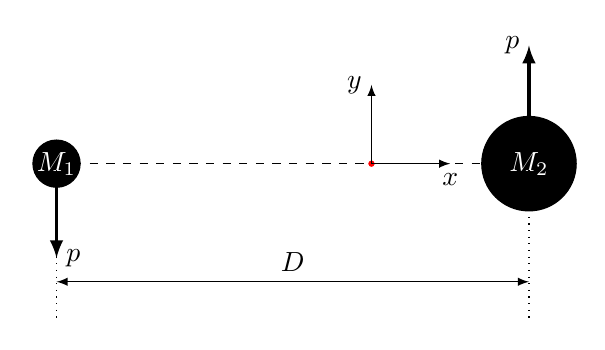
\begin{tikzpicture}
          % line connecting BHs
          \draw[dashed] (-4,0) -- (2,0);
          \filldraw[color=white, fill=red] (0,0) circle (0.05);
        
          % small BH
          \filldraw[fill = black] (-4,0) circle (0.3);
          \draw[very thick,-latex] (-4,0) -- (-4,-1.2);
          \node[anchor=west] at (-4,-1.2) {$p$};
          \node[color=white] at (-4,0) {$M_1$};
          
          % big BH
          \filldraw[fill = black] (2,0) circle (0.6);
          \draw[very thick,-latex] (2,0) -- (2,1.5);
          \node[anchor=east] at (2,1.5) {$p$};
          \node[color=white] at (2,0) {$M_2$};
        
          % length
          \draw[dotted] (2,0) -- (2,-2);
          \draw[dotted] (-4,0) -- (-4,-2);
          \draw[latex-latex] (-4,-1.5) -- (2,-1.5);
          \node[anchor=south] at (-1,-1.5) {$D$};
          
          % axes
          \draw[-latex] (0,0) -- (0,1);
          \node [anchor=east] at (0,1) {$y$};
          \draw[-latex] (0,0) -- (1,0);
          \node[anchor=north] at (1,0) {$x$};
\end{tikzpicture}
    \caption{Schematic diagram of the initial BH binary setup for 
    an arbitrary configuration in one of the sequences.}
    \label{bhkick:fig:bh-setup}
\end{figure}

We have parametrized the configurations within a sequence by their
initial tangential momentum $p$, but we would like to measure the
eccentricity of these configurations. Unfortunately, there is no
gauge-invariant measure of eccentricity~\cite{Loutrel:2018ydu} and the
ambiguity in any definition is particularly pronounced in the late
stages of inspiral from which our simulations start. Following
Ref.~\cite{Sperhake:2007gu}, we use the formalism in
Ref.~\cite{Memmesheimer:2004cv} to obtain a PN estimate for the
eccentricity. Note that this formalism has three eccentricity
parameters---$e_t$, $e_r$ and $e_\phi$---and employs two
different types of coordinates: ADM-like and harmonic. The choice of
which parameter and coordinate type to use is somewhat arbitrary.
We mostly focus on the eccentricity parameter $e_t$ in harmonic coordinates\footnote{
The ADM-like estimate of Ref.~\cite{Memmesheimer:2004cv} differs
by only a few percent for $e_t \lesssim 0.8$, and
would not significantly alter our results.} 
as in Ref.~\cite{Sperhake:2019wwo}. This estimate should be 
taken with a pinch of salt due to the relatively small initial binary 
separations $D$ in our simulations. Furthermore, $e_t$ has an infinite 
gradient as a function of the initial orbital angular momentum
in the quasicircular limit (see Fig.~1 in Ref.~\cite{Sperhake:2007gu}),
such that values of $e_t\lesssim0.1$ are difficult to realize in practice,
unless the BHs start from large initial distance.
In the head-on limit $e_t$ diverges, and a Keplerian/Newtonian
interpretation ceases to be valid. Despite these shortcomings, this 
estimate provides us with a helpful approximation of the eccentricity
and a criterion to quantify deviations away from quasicircularity.

The sequences considered in this work are given in
Table~\ref{bhkick:tab:sequences}.  Note that there are two sequences
corresponding to the mass ratio $q=1/2$.  The sequence \texttt{lq1:2}
has a longer inspiral phase compared to the other sequences. For the
nearly quasicircular configurations, the binary completes about six
orbits before merger in the \texttt{lq1:2} sequence, and about three
orbits in all other sequences. The longer sequence of simulations was
conducted in order to identify any possible artifacts in the shorter
sequences due to the exclusion of the earlier inspiral phase. In
addition to the labeling of sequences in Table~\ref{bhkick:tab:sequences},
we refer to individual simulations within a sequence by appending
``\texttt{-p}'' to the sequence label followed by a four digit integer
which is given by $10^3p/M$ truncated appropriately; for example,
\texttt{sq1:2-p0100} denotes the simulation in sequence
\texttt{sq1:2} with initial tangential momentum $p = 0.1M$.



\begin{table}[t]
    {
    \caption{Sequences of binary BH configurations studied in this 
    work with their mass ratio, binding energy $E_{\mathrm{b}}/M$,
    and the GW extraction radius $r_{\rm ex}$.
    For reference, we also
    list for each sequence the kick velocities $v_c$ in the
    quasicircular limit. These values agree, within the numerical
    uncertainties, with the results of
    Ref.~\cite{Gonzalez:2006md}.}
    \centering
    %\begin{ruledtabular}
    \begin{tabular}{cccccc} \hline
        Sequence & Code & $q$ & $E_{\mathrm{b}}/M$ & $r_{\mathrm{ex}}/M$ 
        & $v_c$ (km/s)\\
        \hline
        \texttt{sq2:3} & \textsc{GRChombo} & $2/3$ & $-0.0113386$ & $88$ & 102 \\
        \texttt{sq1:2} & \textsc{Lean} & $1/2$  & $-0.0106964$ & $80$ & 149\\
        \texttt{lq1:2} & \textsc{Lean} & $1/2$ & $-0.0090858$ & 80 & 150 \\
        \texttt{sq1:3} & \textsc{GRChombo} & $1/3$ & $-0.0093684$ & $65$ & 178 \\
        \hline
    \end{tabular}
    %\end{ruledtabular}
    }
    \captionsetup{justification=justified}
    \label{bhkick:tab:sequences}
\end{table}

\subsection{Diagnostics}
For all simulations, we have extracted values of the Weyl scalar $\Psi_4$ 
on spheres of finite coordinate radius given in Table \ref{bhkick:tab:sequences} 
for each sequence. We also computed the dominant terms in the multipolar
decomposition,
\begin{equation}\label{bhkick:eq:psi4-multipoles}
    \Psi_4(t,r,\theta,\phi) = \sum_{\ell=2}^\infty\sum_{m=-\ell}^{\ell} 
    \psi_{\ell, m}(t,r)\left[{}_{-2}Y^{\ell,m}(\theta,\phi)\right],
\end{equation}
where ${}_{-2}Y^{\ell,m}$ are the usual spin-weight $-2$ spherical 
harmonics.

Our main diagnostics are the energy, linear momentum and angular momentum 
radiated in GWs, which are computed directly from the 
extracted $\Psi_4$ values on the spheres using standard methods. For
completeness, we reproduce the formulae here.

The radiated energy $E^{\rad}$ is given by
\cite{Campanelli:1998jv,Lousto:2007mh}
\begin{equation}
    E^{\rad}(t) = \lim_{r\to\infty}\frac{r^2}{16\pi}\int_{t_0}^t\rmd t^\prime
    \oint_{S^2_r}\rmd\Omega\,\left|\int_{-\infty}^{t^\prime}\rmd t^{\prime\prime}\,
    \Psi_4\right|^2.\label{bhkick:eq:Erad}
\end{equation}
The radiated linear momentum $\mathbf{P}^{\rad}$ is given by
\begin{equation}
    \mathbf{P}^{\rad}(t) = \lim_{r\to\infty}\frac{r^2}{16\pi}
    \int_{t_0}^t\rmd t^\prime\oint_{S^2_r}\rmd\Omega\,
    \hat{\mathbf{e}}_r\left|\int_{-\infty}^{t^\prime}\rmd t^{\prime\prime}\,
    \Psi_4\right|^2,\label{bhkick:eq:Prad}
\end{equation}
where $\hat{\mathbf{e}}_r$ is the flat-space unit radial vector
\begin{equation}
    \hat{\mathbf{e}}_r = (\sin\theta\cos\phi,\sin\theta\sin\phi,\cos\theta).
\end{equation}
Finally, the radiated angular momentum $\mathbf{J}^{\rad}$ is given by
\begin{equation}
    \mathbf{J}^{\rad}(t) = - 
    \lim_{r\to\infty}\frac{r^2}{16\pi}\mathrm{Re}\int_{t_0}^{t}\rmd t^\prime
    \left\{\oint_{S^2_r}\left(\int_{-\infty}^{t^\prime}\rmd t^{\prime\prime}\,
    \bar{\Psi}_4\right)\right.
    \left. \times\hat{\mathbf{J}}\left(\int_{-\infty}^{t^\prime}
    \rmd t^{\prime\prime}\int_{-\infty}^{t^{\prime\prime}}
    \rmd t^{\prime\prime\prime}\,\Psi_4\right)\,\rmd\Omega\right\},
    \label{bhkick:eq:Jrad}
\end{equation}
where the angular momentum operator $\hat{\mathbf{J}}$ for spin weight 
$s=-2$ is given by
\begin{equation}
    \hat{\mathbf{J}}=\left(\mathrm{Re}\,\hat{\mathbf{J}}_+,\mathrm{Im}\,
    \hat{\mathbf{J}}_+,\frac{\partial}{\partial\phi}\right)\,,
\end{equation}
and
\begin{equation}
    \hat{\mathbf{J}}_+=\mathrm{e}^{\mathrm{i}\phi}\left(\mathrm{i}
    \frac{\partial}{\partial\theta} - \cot\theta\frac{\partial}{\partial\phi} 
    + 2\mathrm{i}\csc\theta\right).
\end{equation}

Additionally, we compute the radiated linear momentum from the multipolar
amplitudes $\psi_{\ell, m}$ in Eq.~\eqref{bhkick:eq:psi4-multipoles} using the 
formulae of Ref.~\cite{Ruiz:2007yx}. From the symmetry of our 
configurations, the $z$ component vanishes identically: $P_z^{\rad}=0$.
For the components in the orbital plane, we write
$P_+^{\rad}=P_x^{\rad}+\mathrm{i}P_y^{\rad}$. Then,
\begin{equation}
     P_+^{\rad}(t) = \sum_{\tl=2}^{\infty}
     \sum_{\tm=-\tl}^{\tl}P_+^{\tl,\tm},
     \label{bhkick:eq:P+rad}
\end{equation}
where
\begin{multline}
    P_+^{\tl,\tm}(t) = \lim_{r\rightarrow \infty}
    \frac{r^2}{8\pi}\int_{t_0}^t\rmd t^{\prime}
    \left\{\left(\int^{t^\prime}_{-\infty}\rmd t^{\prime\prime}\, 
    \psi_{\tl,\tm}\right)\right. \\
    \left.\times\left(\int_{-\infty}^{t^\prime} 
    \left[a_{\tl,\tm}\bar{\psi}_{\tl,\tm+1}+ 
    b_{\tl,-\tm}\bar{\psi}_{\tl-1,\tm+1}
    -\,b_{\tl+1,\tm+1}\bar{\psi}_{\tl+1,\tm+1}\right]
    \rmd t^{\prime\prime}\right)\right\},
    \label{bhkick:eq:Plmrad}
\end{multline}
and the coefficients $a_{\ell,m}$ and $b_{\ell,m}$ are given by
%
\begin{align}
    a_{\ell, m} &= \frac{\sqrt{\left(\ell - m\right)\left(\ell +
    m+1\right)}}{\ell\left(\ell + 1\right)},\\
    b_{\ell, m} &= \frac{1}{2\ell}\sqrt{\frac{\left(\ell - 2\right) 
    \left(\ell + 2\right) \left(\ell + m\right) \left(\ell + m - 
    1\right)}{\left(2\ell - 1\right)\left(\ell + 1\right)}}.
\end{align}
%
We will find it helpful to define the partial sums,
%
\begin{align}
    P_+^{\tl} &= \sum_{\tm = -\tl}^{\tl} P_+^{\tl,\tm},\\
    P_+^{\leq\tl} &= \sum_{\tl^\prime=2}^{\tl} P_+^{\tl^\prime}. 
    \label{bhkick:eq:partialkick}
\end{align}
%
In practice, we do not evaluate the limit in Eqs.~\eqref{bhkick:eq:Erad}, 
\eqref{bhkick:eq:Prad}, \eqref{bhkick:eq:Jrad} and \eqref{bhkick:eq:Plmrad}, but rather just 
evaluate them at the finite extraction radius $r=r_{\mathrm{ex}}$, as given 
in Table \ref{bhkick:tab:sequences}. A discussion of the error this introduces is 
given in the following section.

In order to exclude the spurious radiation inherent in Bowen-York initial 
data, we start the integration in Eqs.~\eqref{bhkick:eq:Erad}, \eqref{bhkick:eq:Prad}, 
\eqref{bhkick:eq:Jrad}, and \eqref{bhkick:eq:Plmrad} at $t_0 = 50M + r_{\mathrm{ex}}$. The 
recoil velocity is computed from the radiated momentum according to 
%
\begin{equation}
    \mathbf{v}=-\frac{\mathbf{P}^{\rad}}{M_{\mathrm{fin}}},
\end{equation}
%
where $M_{\mathrm{fin}}$ is the mass of the BH merger remnant. The 
quantity $M_{\mathrm{fin}}$ can be computed using energy balance:
\begin{equation}
    M_{\mathrm{fin}} = M_{\mathrm{ADM}} - \tilde{E}^{\rad}\,,
\end{equation}
where $\tilde{E}^{\rm rad}$ denotes the radiated energy
{\it including} the spurious radiation.
We similarly compute the spin of the final BH $\chi_{\mathrm{fin}}$ (which,
by symmetry, must be in the $z$ direction) using the radiated angular 
momentum:
\begin{equation}
    \chi_{\mathrm{fin}} = \frac{L-J^{\rad}_z}{M_{\mathrm{fin}}^2},
\end{equation}
where the initial angular momentum is $L=pD$. For \textsc{Lean} simulations, 
we have compared $M_{\rm fin}$ and $\chi_{\rm fin}$ with the
corresponding values derived from the apparent horizon properties,
and find agreement to within $\leq 0.1\,\%$.


%=============================================================================
\section{Results}
%
\label{bhkick:sec:results}
%
\begin{figure*}[t]
    \subfloat
    {
        \includegraphics[width=0.48\linewidth]{bhkick/kick-q1.5-wlabel.pdf}
    }
    \hfill
    \subfloat
    {
        \includegraphics[width=0.48\linewidth]{bhkick/kick-q3-wlabel.pdf}
    }
    \hspace{0 mm}
    \subfloat
    {
        \includegraphics[width=0.48\linewidth]{bhkick/kick-q2-wlabel.pdf}
    }
    \hfill
    \subfloat
    {
        \includegraphics[width=0.48\linewidth]{bhkick/kick-q2l-wlabel.pdf}
    }
    \caption{For each sequence of simulations in Table \ref{bhkick:tab:sequences}:
    Top panel: the recoil velocity $v$ is plotted as a function 
    of the initial tangential momentum $p/M$. The individual curves 
    represent the total kick $v_\mathrm{tot}$ (blue, solid), the 
    contribution to the kick from $\ell=2$ modes of $\Psi_4$, $\psi_{2,m}$, 
    only in Eqs.~(\ref{bhkick:eq:P+rad})--(\ref{bhkick:eq:Plmrad}) $v_{\ell=2}$ 
    (red, dashed), and the contributions to the kick from 
    $P_+^{\leq \tilde{\ell}^\prime}$ defined in Eq.~\eqref{bhkick:eq:partialkick}
    $v_{\tilde{\ell}\leq\tilde{\ell}^\prime} $ for $\tilde{\ell}^\prime=2$ 
    (orange, dotted), $\tilde{\ell}^\prime=3$ (green, dot-dashed) 
    and $\tilde{\ell}^\prime=4$ (purple, long dot-dashed). 
    Our estimate of the eccentricity (see Sec.~\ref{bhkick:sec:configs}) is 
    provided on the upper horizontal axis.
    Bottom panel: The final BH spin $\chi_{\mathrm{fin}}$ 
    (black, solid) and the energy radiated in GWs $E^\rad$ (gold, dashed) 
    are also plotted as functions of $p/M$. For both curves, the 
    individual simulations performed for this analysis are shown by 
    $\times$ symbols.}
    \label{bhkick:fig:kicks2}
\end{figure*}
%
Using the framework summarized in the previous section,
we have simulated four sequences of nonspinning BH binaries,
characterized by their mass ratio (\ref{bhkick:eq:mass-ratio})
and binding energy (\ref{bhkick:eq:binding-energy}).
The parameters of these sequences are listed in Table~\ref{bhkick:tab:sequences}.
We have selected our mass ratios such that they cover the
regime of maximum recoil, realized for $\eta=0.195$ or
$q=1/2.77$ (cf. Fig.~\ref{bhkick:fig:quasicircular-fit-comparison}).
Recall that sequences \texttt{sq2:3}, \texttt{sq1:2} and \texttt{sq1:3}
complete about three orbits and sequence \texttt{lq1:2} completes
about six orbits, respectively, in the quasicircular limit.

Our main results are displayed in Fig.~\ref{bhkick:fig:kicks2}, where we plot
for all sequences the total recoil speed $v_{\rm tot}$, various
truncations of the multipolar contributions to the total recoil
according to Eqs.~(\ref{bhkick:eq:P+rad})--(\ref{bhkick:eq:partialkick}), the
total radiated GW energy $E^{\rm rad}$ and the dimensionless spin
$\chi_{\rm fin}$ of the BH resulting from the merger.

Let us first focus on the total recoil $v_{\rm tot}$, displayed in each
of the figure's top panels as the blue solid line.  For each mass
ratio, the global maximum of the kick velocity is realized for
moderate eccentricities
$e_t\approx 0.5$.
We also illustrate this kick variation in
Fig.~\ref{bhkick:fig:quasicircular-fit-comparison}, where
the solid blue curve shows the
quasicircular kick as a function
of the symmetric mass ratio $\eta$ according to
Fit 3 in Table V of Ref.~\cite{Healy:2017mvh}. The velocity ranges
obtained for our eccentric binaries are
overlayed as the vertical bars for each of our sequences.
The bar for each constant-$\eta$ sequence
is obtained by starting at the quasicircular limit on the 
right of each panel in Fig.~\ref{bhkick:fig:kicks2} and identifying
the minimum and maximum of $v(p)$, excluding the 
plunge regime to the left of the global maximum.

For our sequences \texttt{sq2:3}, \texttt{sq1:2} and
\texttt{lq1:2}, the 
magnification of the kick through moderate values
of the orbital eccentricity is similar to the
enhancement by up to 25\,\% reported in
Ref.~\cite{Sperhake:2019wwo}
for the so-called superkick configurations
\cite{Gonzalez:2007hi,Campanelli:2007cga}.
For \texttt{sq1:3} the effect is milder, with a
$\sim 12\,\%$ amplification, but still well above
the uncertainty estimates of our simulations.
On the other hand, as evidenced by the oscillatory pattern
of the function $v(p)$ in Fig.~\ref{bhkick:fig:kicks2}, appropriate
nonzero values of the eccentricity can also
lead to a {\it reduction} of the maximum kick at a given mass ratio
by $\sim 10\,\%$.
This overall modification of the gravitational recoil
in the merger of eccentric, nonspinning BH binaries
is the first main result of our study.

\begin{figure}[t]
    \centering
    \includegraphics[width=0.7\columnwidth]{bhkick/quasicircular-fit2.pdf}
    \caption{The range of recoil velocities obtained for each sequence
    is plotted against the symmetric mass ratio $\eta$. Note that for
    each sequence we exclude the configurations with 
    $p<p_{\text{max}}$ (i.e. the head-on limit), where 
    $p=p_{\text{max}}$ is the tangential momentum that maximizes the kick.
    The three short sequences are marked in gold and the long sequence is 
    marked in red (dashed). A fitted formula for the quasicircular
    kick as a function of $\eta$ from Ref.~\cite{Healy:2017mvh} is
    also shown in blue for comparison. 
    }
    \label{bhkick:fig:quasicircular-fit-comparison}
\end{figure}

Besides the global maximum, we also note a number of local minima and
maxima in the kick velocity as we vary the eccentricity in
Fig.~\ref{bhkick:fig:kicks2}. For all mass ratios $(q=2/3,\,1/2,\,1/3)$ we
see about five 
local extrema in $v(p)$ in our three short sequences,
corresponding to the two upper panels and the bottom-left panel.
We notice a similar, albeit less pronounced,
oscillatory pattern in the functions
$E_{\rm rad}(p)$ and $\chi_{\rm fin}(p)$ for the radiated
energy and final spin in the lower subpanels in
Fig.~\ref{bhkick:fig:kicks2}. Our results display no systematic
correlation, however, between the extrema of the respective
quantities; neither global nor local extrema in $v$,
$E_{\rm rad}$ or $\chi_{\rm fin}$ coincide in
magnitude or their eccentricity values.
We believe this diversity is due to the qualitatively
different dependence of the radiated quantities on the
GW multipoles: overlaps of {\it different} multipoles for the
kick, a sum of terms $\propto \psi_{lm}^2$ for the energy,
and the interaction of first and second time integrals
for the angular momentum in Eq.~(\ref{bhkick:eq:Jrad}).

We added
to our study the $q = 1/2$ sequence of longer BH binary inspirals to
investigate whether these anomalies in $v=v(p)$ might merely result
from ignoring in our simulations the earlier inspiral phase. The
remarkable outcome of this test, however, is that the oscillatory
behavior in the kick as a function of eccentricity is \emph{more}
pronounced in the long sequence.  The solid blue curve in the
bottom-right panel of Fig.~\ref{bhkick:fig:kicks2} displays significantly more
rapid oscillations in the eccentricity regime
$0.2\lesssim e_t \lesssim 0.4$ as compared to the shorter inspiral
sequences.  This oscillatory behavior, and the apparent increase in
the number of oscillations as we increase the initial separation of
the BHs, is the second of our results.

We next attempt to gain insight into the origin of this
behavior. For this purpose, we have computed the
multipolar contributions to the total kick according to
Eqs.~(\ref{bhkick:eq:Plmrad})--(\ref{bhkick:eq:partialkick}). The resulting
velocities are displayed in Fig.~\ref{bhkick:fig:kicks2} by the additional
dashed, dotted and dash-dotted curves. 
Here, the curves labeled
$v_{\ell=2}$ have been computed from the $\ell=2$ modes of $\Psi_4$
($\psi_{2,m}$ only) in Eqs.~(\ref{bhkick:eq:P+rad})-(\ref{bhkick:eq:Plmrad}).
We computed this additional contribution (red dashed curves in the
figure) to determine whether the oscillatory behavior is also present
in the pure quadrupole signal. The answer is yes: the oscillations are
clearly perceptible in $v_{\ell=2}$, even though they are a bit milder
than in the total kick $v_{\mathrm{tot}}$. Considering all
(cumulative) multipolar contributions shown in Fig.~\ref{bhkick:fig:kicks2},
we notice the following behavior:
%
\begin{enumerate}
 \item The oscillatory dependence of the kick on eccentricity
       is present at any level of truncating the multipolar
       contributions in the cumulative sum (\ref{bhkick:eq:partialkick}).
 \item The partial sum of the kick up to $\tilde{\ell}=4$
       barely differs from the total kick, indicating that
       higher-order overlap terms do not significantly
       contribute to the kick.
 \item The higher-order contributions $\tilde{\ell}>2$
       to the cumulative kick (\ref{bhkick:eq:partialkick})
       systematically decrease the kick, counteracting
       the pure quadrupole contribution $v_{\ell=2}$.
\end{enumerate}
%
In short, we have not identified any specific multipoles
dominating the variation in the kick function $v=v_{\mathrm{tot}}(p)$.

In our search for an explanation, we turn next to the infall direction
of the BH binary just before merger.
%
%
\begin{figure*}[t]
    \subfloat%[][$v$ against $\vartheta$]
    {
    % \centering
    \includegraphics[width=0.5\columnwidth]{bhkick/kick-theta.pdf}
    \label{bhkick:fig:kick-theta}
    }
    \hfill
    \subfloat%[][$\vartheta_\text{extrema}$ against $m$]
    {
    % \centering
    \includegraphics[width=0.5\columnwidth]{bhkick/theta-extrema.pdf}
    \label{bhkick:fig:theta-extrema}
    }
    \caption{
    Plots involving the angle of the kick $\vartheta$ for 
    all sequences. In the left panel we plot the BH recoil 
    velocity $v$ against $\vartheta$. In the right panel we plot the location of the local extrema $\vartheta_\text{extrema}$ 
    of the left panel against the index of the extrema $k$ counting rightwards from
    the global maximum on the left.
    }
    \label{bhkick:fig:theta-plots}
\end{figure*}
%
A well-known feature of the superkicks generated in the inspiral
of BHs with opposite spins $\boldsymbol{S}_1=-\boldsymbol{S}_2$
pointing in the orbital
plane is the sinusoidal variation with the initial azimuthal angle
of the spin vectors; cf.~Fig.~4 in Ref.~\cite{Bruegmann:2007zj}.
The initial orientation of the spins can, alternatively, be
interpreted as a measure for the angle between the in-plane
spin components and the BH binary's infall direction at merger
\cite{Lousto:2009ka}. The superkick is therefore commonly
determined by simulating otherwise identical BH binary configurations
for different values of this angle and fitting the resulting data
with a cosine function; see, e.g.,~Sec.~III A in
Ref.~\cite{Sperhake:2019wwo}. For the eccentric, nonspinning BH
binaries considered in this work, it is the
initial apsis (either a periapsis or an apoapsis)
that defines a reference direction. Unfortunately,
neither the apsis nor a ``binary infall direction''
are rigorously defined
quantities in the strong-field regime of general relativity,
and we consider instead the orientation of the final
kick relative to the $x$ axis, defined by
%
\begin{equation}
  \tilde{\vartheta} = \mathrm{arg}(v_x + \mathrm{i}v_y)\,.
\end{equation}
For convenience, we define
\begin{equation}
    \vartheta = \tilde{\vartheta} + 2n\pi,
\end{equation}
where $n\geq 0$ is chosen minimally for each configuration in order to obtain
$\vartheta$ as a monotonic function of the initial tangential momentum $p$
for each sequence. We will interchangeably refer to $\vartheta$ 
and $\tilde{\vartheta}$ as the angle of the kick.
%
Since all of our simulations start with the BHs located on the $x$
axis with purely tangential initial momentum $\mathbf{p}=(0,\pm p,0)$
(Fig.~\ref{bhkick:fig:bh-setup}), the $x$ direction can be regarded as the
initial direction of the apoapsis. If we furthermore interpret the
gravitational recoil to be predominantly generated by the excess
beaming of the GWs in the direction of the smaller and faster BH (see
Fig.~3 in Ref.~\cite{Wiseman:1992dv}) during the short merger phase,
the kick direction can serve as an approximate measure for the infall
direction of the binary. 

We can test this prediction by computing the kick magnitude
as a function of the angle $\vartheta$; if correct, we would
expect a periodic variation with a period close to $2\pi$.
We do not expect an exact $2\pi$ periodicity because the
relevant periapsis (or apoapsis) direction should be the last one before merger,
and will shift away from the $x$ axis during the inspiral
due to 
apsidal precession---the BH analog
of Mercury's perihelion precession around the Sun. More
specifically, we would expect deviations from a $2\pi$ periodicity
to be more pronounced for longer inspirals, i.e.,~lower eccentricity
and/or larger initial separations, but only mildly
dependent on the mass ratio $q$.
Quite remarkably, all of these
features are borne out by the functions $v = v(\vartheta)$
displayed for our four sequences in the left panel of 
Fig.~\ref{bhkick:fig:theta-plots}
and the location of the extrema in this plot shown in 
the right panel of Fig.~\ref{bhkick:fig:theta-plots}.
For all sequences we observe the same approximate $2\pi$ periodicity,
with deviations from this value increasing at larger
$\vartheta$, i.e.~for longer inspirals.
Note also that $\vartheta=-\pi$ in the head-on limit, as expected
for our initial configurations, that start with the heavier BH
located on the positive $x$ axis.

While short of a rigorous proof, this result provides considerable
evidence in favor of interpreting the oscillatory dependence of the
kick on the eccentricity as a consequence of the corresponding
variation in the infall direction as measured relative to the last
apoapsis (or periapsis) of the eccentric binary. This interpretation
also explains why the longer sequence \texttt{lq1:2} exhibits more
oscillations than the shorter sequences \texttt{sq1:3}, \texttt{sq1:2}
and \texttt{sq2:3}. Let us consider for this purpose two binary
configurations that only differ by a tiny amount of eccentricity
$\delta e$. The longer the inspiral phase, the more time these two
binaries have to build up a considerable phase difference and, hence,
a different kick and merger GW signal. Note the potentially dramatic
consequences of this behavior for the GW emission from eccentric
binaries over astrophysical time scales. For long astrophysical
inspirals retaining some eccentricity near merger,
the kick and GW merger signal should exhibit critical dependence on
the eccentricity. In terms of our Fig.~\ref{bhkick:fig:kicks2}, the function
$v=v(e_t)$ would display a huge number of oscillations rather than the
handful observed in our case, and the resulting curve would look like
a ``band'' rather than a single line. Within the band, a very small
change $\delta e_t$ in eccentricity can produce a finite change in the
kick and merger waveform.

As indicated by our analysis of the multipolar contributions
to the total recoil, the variations in the GW signal are of a
complex nature. We defer a more comprehensive analysis of
the GW pattern to future work, but merely illustrate with an 
example the type of variations that are encountered.
For this purpose, we show in Fig.~\ref{bhkick:fig:psi4modes}
the $(\ell,m)=(2,2)$ and $(3,3)$ multipoles of the
GW signal around merger for the configurations \texttt{lq1:2-p0537} 
and \texttt{lq1:2-p0567}, corresponding to a local minimum and 
maximum in the
kick, respectively; cf.~the bottom-right panel of Fig.~\ref{bhkick:fig:kicks2}. In Fig.~\ref{bhkick:fig:psi4modes},
the time has been shifted such that $\Delta t =0$ corresponds
to the first occurrence of a common apparent horizon. The main
difference perceptible in the figure is the relative phase shift of
the (3,3) mode relative to the dominant quadrupole (2,2). For the
case $p=0.567M$ with maximal kick, the global peaks of both multipoles
are aligned, whereas for $p=0.537M$ with minimal kick, the global peak
of the $(2,2)$ mode coincides with a minimum in $(\ell,m)=(3,3)$. We
have made similar observations for other pairs of modes such as
$(2,2)$ and $(2,1)$, and find these pairs to dominate the oscillatory
variation in the multipolar series expansion (\ref{bhkick:eq:partialkick}).
%
\begin{figure}[t]
    \centering
    \includegraphics[width=0.7\columnwidth,clip=true]{bhkick/mode-kick-extrema.pdf}    
    \caption{The real parts of the $(\ell,m)=(2,2)$ and $(3,3)$ modes of $\Psi_4$
             are shown as functions of time for the two binaries
             of sequence \texttt{lq1:2} with $p/M=0.537$ and $p/M=0.567$,
             resulting in kick velocities of $v = 128$
             and $173\,{\rm km/s}$, respectively.
            }
             \label{bhkick:fig:psi4modes}
\end{figure}
%



%=============================================================================
\section{Conclusions}
\label{bhkick:sec:concl}
%
In this paper we have studied the gravitational recoil and GW emission
of sequences of nonspinning BH binaries with mass ratios $q=2/3$,
$1/2$ and $1/3$,
and eccentricity varying from the quasicircular to the head-on limit.
For this purpose we have evolved $274$ configurations
with the {\sc GRChombo} and {\sc Lean} codes. Both codes yield
convergent results for the recoil with a total error budget of
$3$-$4\,\%$ and exhibit excellent agreement, well within this uncertainty
estimate, for a verification configuration simulated with both codes.
In order to estimate the impact of variations in the overall length
of the inspirals, we have evolved two sequences for the case $q=1/2$ which
complete about three and six orbits, respectively, in the quasicircular limit.

The findings of our study are summarized as follows.
%
\begin{enumerate}
 \item For all sequences, the total recoil reaches
 a global maximum for moderate eccentricities $e \sim 0.5$.
 As in the case of the enhancement of superkicks studied
 in Ref.~\cite{Sperhake:2019wwo}, the maximum kick is
 enhanced by up to about $25\,\%$ relative to the value obtained
 for quasicircular configurations.
 %
\item Besides this global maximum, we observe an oscillatory
  dependence of the kick $v$ as a function of eccentricity, with
  several local minima and maxima in the function $v = v(e)$. Appropriate
  nonzero values of the eccentricity can lead to a
  {\it reduction} of the kick by $\sim 10\,\%$ relative to the quasicircular
  value instead of an increase. By
  splitting the kick into separate multipolar contributions, we notice
  that this oscillatory dependence is already present, albeit in a
  slightly weaker form, when we consider only quadrupole terms in the
  series expansion \eqref{bhkick:eq:P+rad}.  Further contributions involving
  $\ell \ge 2$ multipoles tend to decrease the overall kick and mildly
  enhance the oscillatory variation; see Fig.~\ref{bhkick:fig:kicks2}.
 %
 \item We interpret this oscillatory variation in the kick
 as a consequence of changes in the angle between the infall
 direction at merger and the apoapsis (or periapsis)
 direction. In the absence of rigorous definitions for either
 of these directions, we approximate this angular variation
 by considering the direction of the final kick and the
 $x$ axis, assuming that the former is related via relativistic
 GW beaming to the infall direction and by taking into account
 that our BHs start on the $x$ axis with zero radial momentum.
 Displayed as a function of this angle, the kick displays
 the expected periodic behavior with a period close to but
 mildly deviating from $2\pi$, presumably due to periapsis
 precession.
 %
 \item We have explored the dependence of this oscillatory behavior
 of the recoil by simulating an additional sequence of eccentric
 binaries with mass ratio $q=1/2$, but less negative binding energy,
 corresponding to about six orbits in the quasicircular limit.
 We find the oscillations in $v=v(e)$ to be more pronounced
 and numerous than in the shorter sequence. We attribute this
 feature to the longer available time window during which otherwise
 identical binaries with tiny differences in the initial
 eccentricity build up a phase difference prior to merger.
 This observation raises the intriguing possibility that the
 total recoil depends highly sensitively on the initial eccentricity.
 %
 \item The variations in the kick velocity are accompanied by
 relative time shifts in the peak amplitudes of subdominant
 multipoles relative to the peaks of the (2,2) mode;
 cf.~Fig.~\ref{bhkick:fig:psi4modes}. For configurations with a large (small)
 kick, the peak amplitude of subdominant multipoles tends to
 be aligned (misaligned) with the quadrupole peak.
\end{enumerate}
%
Our findings point to a variety of future investigations. While our
simulations indicate an increased sensitivity of the GW merger signal
to the initial eccentricity for larger initial separations
(i.e.~longer inspirals), it is not clear how this will be affected by
the circularizing nature of GW emission. In this context, it will also
be important to analyze in more quantitative terms the differences in
the GW signals and possible implications for parameter inference in GW
observations. A thorough investigation of long eccentric inspirals on
astrophysical time scales will likely require PN methods and may
benefit greatly from a multi-time-scale analysis in phase space, as
applied to spin-precessing BH binaries in
Refs.~\cite{Kesden:2014sla,Gerosa:2015tea} or to the dynamics of
binary systems in external gravitational background potentials in
Refs.~\cite{Hamilton:2019a,Hamilton:2019b}. If there is a single
conclusion to draw from the results of this work, it is the
surprisingly rich phenomenology of the GW signals of eccentric compact
binaries---even in the absence of spins---which merits as much as it
requires further investigation.

% %=============================================================================
% \begin{acknowledgments}
% %
% We thank Michalis Agathos, Vishal Baibhav, Vitor Cardoso, Thomas
% Helfer, and Nicholas Speeney for useful discussions. 
% We also thank Chris Moore, Carlos Lousto and Juan Calder\'on 
% Bustillo for helpful comments on this manuscript.
% M.R. thanks the
% GRChombo collaboration \cite{GRChomboWebsite} for their code
% development, and particularly Katy Clough and Tiago Fran\c{c}a. M.R. is
% supported by a Science and Technology Facilities Council (STFC)
% studentship. U.S. is supported by the European Union’s H2020 ERC
% Consolidator Grant ``Matter and strong-field gravity: new frontiers in
% Einstein's theory'' Grant No.~MaGRaTh--646597, and the STFC
% Consolidator Grant No. ST/P000673/1. E.B. is supported by NSF Grant
% No. PHY-1912550, NSF Grant No. AST-2006538, NASA ATP Grant No.
% 17-ATP17-0225 and NASA ATP Grant No. 19-ATP19-0051. This work has
% received funding from the European Union's Horizon 2020 research and
% innovation programme under the Marie Sk\l odowska-Curie Grant
% No.~690904. This work was supported by the GWverse COST Action
% CA16104, ``Black holes, gravitational waves and fundamental physics''.
% %
% Computational work was performed on
% the San Diego Supercomputer Center Comet and Texas Advanced Computing 
% Center (TACC) Stampede2 clusters at the University of California San Diego 
% and the University of Texas at Austin (UT Austin), respectively, through
% NSF-XSEDE Grant No.~PHY-090003; the Cambridge Service for Data 
% Driven Discovery (CSD3) system at the University of Cambridge 
% through STFC capital Grants No.~ST/P002307/1 and No.~ST/R002452/1,
% and STFC operations Grant No.~ST/R00689X/1;
% the TACC Frontera cluster at UT Austin; and
% the JUWELS cluster at GCS@FZJ, Germany through PRACE Grant No.~2020225359.

% \end{acknowledgments}
% %===============



\section{Numerical accuracy}
\label{bhkick:sec:accuracy}
\begin{figure*}[t]
    \subfloat%[\textsc{GRChombo}]
    {
        \includegraphics[width=0.48\linewidth]{bhkick/grchombo-convergence5.pdf}
        %\label{bhkick:fig:grchombo-convergence}
    }
    \hfill
    \subfloat%[\textsc{Lean}]
    {
        \includegraphics[width=0.48\linewidth]{bhkick/lean-convergence4.pdf}
        %\label{bhkick:fig:lean-convergence}
    }
    \caption{For each code, we show convergence plots for the
      accumulated linear momentum radiated from \textsf{sq1:2-p0100}
      by plotting the BH recoil velocity in the bottom panels. The
      Richardson extrapolated curve, $v_{\mathrm{Rich4}}$, assuming
      fourth-order convergence, is also shown in the bottom panel. The
      grid configurations are given in Table~\ref{bhkick:tab:grchombo-grids}
      for \textsc{GRChombo} and in Table~\ref{bhkick:tab:lean-grids} for
      \textsc{Lean}. The top panel shows the difference between the
      configurations along with rescalings corresponding to fourth- and
      fifth-order convergence. The inset shows a magnification of the
      right side of the plot: the final value of the recoil
      velocity is what we show in Fig.~\ref{bhkick:fig:kicks2}.} 
    \label{bhkick:fig:convergence}
\end{figure*}
As in Ref.~\cite{Sperhake:2019wwo}, the uncertainty in our numerical results 
for the recoil velocities has two predominant contributions: the 
discretization error and the finite extraction radii for the Weyl scalar
$\Psi_4$.

To estimate the uncertainty arising from the latter, we have selected a
representative sample of the simulations from each sequence and extrapolated 
the cumulative radiated momentum to infinity from about six extraction
radii in the range $r_{\rm ex}/2 \le r_{\rm ex}$ 
using a Taylor series in $1/r$ as in 
Ref.~\cite{Sperhake:2011zz}. We report the results from the finite 
extraction radii given in Table~\ref{bhkick:tab:sequences} and estimate the 
error by comparing with the linear-order extrapolation.
For both codes, we estimate that the contribution from this error is about
2\% 
for all sequences.

In order to estimate the error contribution from finite differencing and
verify that our codes give consistent results, we have performed simulations
of \texttt{sq1:2-p0100} (the binary in sequence \texttt{sq1:2} with 
$p/M = 0.1$) with both codes. We discuss the analyses of the convergence
of each code separately before comparing.

\subsection{\textsc{GRChombo} convergence}
\begin{table}[b]
{   
    \caption{Grid configurations used for \textsc{GRChombo} simulations.
    As explained in Sec.~\ref{bhkick:sec:grchombo} and Appendix \ref{bhkick:sec:tagging},
    the total 
    number of refinement levels is $L+1$, the number of cells along each
    dimension on the coarsest level is $N$, $t_R$ is the regridding 
    threshold value, $b$ is the BH tagging buffer parameter
    that we
    set proportional to the mass $M_i$ ($i=1,\,2$)
    of the nearest BH for all configurations except R4, 
    and $h_L$ denotes the grid spacing.
    }
    \centering
    %\begin{ruledtabular}
    \begin{tabular}{lcccccc}\hline
        Label & $L$ & $N$ & $t_R$ & $b$ & $h_L/M_1$ & tagging\\
        \hline
        R1 & 7 & 320 & 0.012 & $0.5M_i$ & 3/80 & Spherical \\
        R2 & 7 & 368 & 0.01043 & $0.5M_i$ & 3/92 & Spherical\\
        R3 & 7 & 416 & 0.00923 & $0.5M_i$ & 3/104 & Spherical\\
        R4 & 7 & 352 & 0.01091 & 0.7 & 3/88 & Box\\\hline
    \end{tabular}
    %\end{ruledtabular}
}
    \label{bhkick:tab:grchombo-grids}
\end{table}
For \textsc{GRChombo}, we have performed the simulations of 
\texttt{sq1:2-p0100} with resolutions $h_L=3M_1/80$, $3M_1/92$ and 
$3M_1/104$, and we refer to the configurations corresponding to these 
resolutions as R1, R2 and R3, respectively.
The full grid configurations 
are given in Table~\ref{bhkick:tab:grchombo-grids} and the results of this 
analysis are shown in the left panel of Fig.~\ref{bhkick:fig:convergence}. Around
merger, at $(t-r_{\rm ex})/M\sim 420$, our results exhibit mild
overconvergence
in the top-left panel of Fig.~\ref{bhkick:fig:convergence}.
The important results for our analysis in Fig.~\ref{bhkick:fig:kicks2},
however, are the final kick values after the merged BH has settled down.
As can be seen from the inset, the convergence here is close to 
fifth order. 
From our convergence 
analysis, the difference between the result obtained from the R1 simulation 
and the more conservative fourth-order Richardson-extrapolated result leads 
to an estimate of the discretization error of about $1\%$. A similar error 
estimate is also obtained for the radiated energy, $E^{\rad}$.
From experience, we have found smaller values for the mass ratio $q<1$ 
more challenging to accurately simulate than larger values, and we 
therefore feel justified in using this error estimate (for a $q=1/2$ 
configuration) as a conservative estimate for the error in the 
\texttt{sq2:3} sequence simulations ($q=2/3$). We therefore used the R1 grid
configuration for this sequence with  $l_1^{\max}=l_2^{\max}=L=7$ 
(both BHs are covered by 
the finest level; see Appendix \ref{bhkick:sec:tagging} for details).

For the \texttt{sq1:3} simulations, we used the R4 grid configuration
(see Table \ref{bhkick:tab:grchombo-grids}) with $l_1^{\max}=L=7$ and
$l_2^{\max}=L-1=6$ (the larger BH is not covered by the finest level:
see Appendix \ref{bhkick:sec:tagging} for details). This corresponds to a
resolution of $h_L=3M_1/88$. We performed a separate convergence
analysis of \texttt{sq1:3-p0089}, which led to an estimated 1\%
discretization error.

Combining both the finite extraction radius and discretization errors, 
our estimate for the total error budget of the \textsc{GRChombo} 
simulations is about $3\%$.


\subsection{\textsc{Lean} convergence}
\begin{table}[b]
    {
    \caption{Grid configurations used for \textsc{Lean} simulations. As 
    explained in Sec.~\ref{bhkick:sec:lean}, the total number of refinement 
    levels is $L+1$, the number of fixed refinement levels is $l_F+1$, 
    $R_0$ is the half-length of the outer grid, $R_L$ is the half-length 
    of one cubic component of the innermost grid, and $h_L$ is the grid 
    spacing on the finest level.}
    \centering
    %\begin{ruledtabular}
    \begin{tabular}{lccccc} \hline
        Label & $L$ & $l_F$ & $R_0$ & $R_L$ & $h_L/M_1$\\
        \hline
        S1 & 7 & 4 & 384 & 1 & 1/20\\
        S2 & 7 & 4 & 384 & 1 & 1/24\\
        S3 & 7 & 4 & 384 & 1 & 1/32\\
        S4 & 7 & 4 & 384 & 1 & 1/28\\ \hline
    \end{tabular}
    %\end{ruledtabular}
    }
    \label{bhkick:tab:lean-grids}
\end{table}

With \textsc{Lean}, we have simulated \texttt{sq1:2-p0100} with
resolutions $h_L = M_1/20$, $M_1/24$ and $M_1/32$. We refer to these
grid configurations as S1, S2 and S3, respectively
(cf. Table~\ref{bhkick:tab:lean-grids}). The right panel of Fig.~\ref{bhkick:fig:convergence}
shows convergence between fourth and fifth order. For simulations in
\texttt{sq1:2}, we used the S2 grid configuration. From the
convergence analysis, the difference between the result obtained from
the S2 simulation and the fourth-order Richardson extrapolation leads
to an estimate of the discretization error of about $1.5\%$.

For the \texttt{lq1:2} simulations, we have undertaken a separate
convergence analysis of \texttt{lq1:2-p0086} using the same grid
setup as in
Table~\ref{bhkick:tab:lean-grids}, but using higher resolutions
$h_L/M_1=1/24$, $1/28$ and $1/32$. We observe convergence close to
fourth order and obtain an error estimate of $1\,\%$ from
the Richardson-extrapolated kick for the medium resolution
$h_L/M_1=1/28$.

In summary, the {\sc Lean} simulations of sequence \texttt{sq1:2} are
performed with resolution grid S2 of Table~\ref{bhkick:tab:lean-grids} and an
error budget of $3.5\,\%$, and those of sequence \texttt{lq1:2} with
grid S4 of Table~\ref{bhkick:tab:lean-grids} and an error budget of $3\,\%$.

\subsection{Comparison between \textsc{GRChombo} and \textsc{Lean}}
\label{bhkick:sec:code-comparison}
\begin{figure}[t]
    {
    \centering
    \includegraphics[width=0.7\columnwidth]{bhkick/grchombo-lean-comparison3.pdf}
    }
    \caption{Comparison between \textsc{GRChombo} and \textsc{Lean} 
    for the accumulated linear momentum radiated in GWs in simulations 
    of \texttt{sq1:2-p0100} with $e_t=0.10$.
    We compare the BH recoil velocity (top panel)
    and the corresponding plus-polarized $\ell=m=2$ strain
    amplitude (bottom panel).
    }
    \label{bhkick:fig:grchombo-lean-comparison}
\end{figure}
A comparison of the recoil velocity computed from \textsc{GRChombo} 
and \textsc{Lean} simulations of \texttt{sq1:2-p0100} with the grid 
configurations R1 and S2 (used for the \texttt{sq2:3} and \texttt{sq1:2} runs) 
respectively, is shown in the top panel of Fig.~\ref{bhkick:fig:grchombo-lean-comparison}.
The eccentricity estimate for this system is $e_t=0.10$. We have chosen
this configuration for two reasons. First, to determine appropriate
resolutions, we had to calibrate our codes' accuracy at the start of
our exploration, which we began in the regime of mild eccentricities to
acquire an intuitive understanding of their behavior. Second, 
configurations with mild eccentricity have a longer inspiral phase
than highly eccentric ones, and therefore impose a stronger requirement
on phase accuracy. A mildly eccentric binary is therefore ideally suited
to obtain a conservative estimate of the numerical accuracy, which is representative across the targeted parameter space.

The final recoil velocities obtained for this configuration with
our two codes differ by about 2\%, which is well within the error budget 
of each code.
We also show the quadrupole contribution
$h^+_{2,2}$ to the `+' polarization strain defined by \cite{Bishop:2016lgv}
\begin{equation}
    h^+_{\ell,m}(t,r)-\mathrm{i}h^\times_{\ell,m}(t,r) 
    = a_{\ell,m} + b_{\ell,m}t + \int_0^t\rmd t^\prime\int_0^{t^\prime}
    \rmd t^{\prime\prime}\psi_{\ell,m}(t^{\prime\prime},r),
    \label{bhkick:eq:strain}
\end{equation}
where the constants $a_{\ell,m}$ and $b_{\ell,m}$ are chosen to minimize 
linear drift,
in the bottom panel of the figure, to better illustrate the agreement
between the codes for these grid configurations.

In Fig.~\ref{bhkick:fig:convergence} the differences between the results of 
different resolutions with \textsc{Lean} are greater than that of
\textsc{GRChombo}. However, we found that \textsc{Lean} entered the 
convergent regime at lower resolutions than GRChombo. This is compatible 
with the observations of Ref.~\cite{Alic:2011gg} that higher resolutions 
were required for convergence with CCZ4 compared to BSSNOK.




%=============================================================================
\section{\textsc{GRChombo} tagging criterion}
\label{bhkick:sec:tagging}
%
%
As explained in Sec.~\ref{bhkick:sec:grchombo}, the regridding is controlled by 
the tagging of cells for refinement in the Berger-Rigoutsos algorithm 
\cite{Berger1991}, with cells being tagged if the tagging criterion $C$ 
exceeds the specified threshold value $t_R$ as given in Table 
\ref{bhkick:tab:grchombo-grids}. For this work, we use the 
tagging criterion

\begin{equation}
    C=
    \begin{cases}
        0, &\text{if }l\geq l_{\mathrm{BH}}^{\max}
        \text{ and } r_{\mathrm{BH}} < (M_{\mathrm{BH}}+b),\\
        \max(C_{\chi},C_{\mathrm{punc}},C_{\mathrm{ex}}),&
        \text{otherwise},
    \end{cases}
\end{equation}

where $l_{\mathrm{BH}}^{\max}$ is a specifiable maximum level parameter 
for each BH (so that it is not unnecessarily over resolved), 
$r_{\mathrm{BH}}$ is the coordinate distance to the puncture, 
$M_{\mathrm{BH}}$ is the mass of the corresponding BH, $b$ is a buffer 
parameter, and $C_\chi$, $C_{\mathrm{punc}}$, and $C_{\mathrm{ex}}$ are 
given as follows:
\begin{enumerate}
    \item 
        $C_{\chi}$ tags regions in which the gradients of the conformal 
        factor $\chi$ become steep. It is given by
        \begin{equation}
            C_{\chi} = h_l\sqrt{\sum_{i,j}\left(
            \partial_i\partial_j\chi\right)^2}\,,
        \end{equation}
        where $h_l$ is the grid spacing on refinement level $l$.
    \item 
        $C_{\mathrm{punc}}$ tags within spheres around each puncture in 
        order to ensure the horizon is suitably well resolved. It is given 
        by
        \begin{equation}
            C_{\mathrm{punc}} = 
            \begin{cases}
                100, &\text{if } r_{\mathrm{BH}} < 
                (M_{\mathrm{BH}}+b) 2^{\max(l_\mathrm{BH}^{\max}-l-1, 2)}, \\
                0, & \text{otherwise}.
            \end{cases}
        \end{equation}
    \item
        $C_{\mathrm{ex}}$ ensures each sphere on which we extract the 
        Weyl scalar $\Psi_4$ is suitably well resolved. It is given by
        \begin{equation}
            C_{\mathrm{ex}} = 
            \begin{cases}
                100, &\text{if } r < 1.2r_{\mathrm{ex}} \text{ and } 
                l < l_{\mathrm{ex}}, \\
                0, & \text{otherwise},
            \end{cases}
        \end{equation}
         where $r$ is the coordinate distance to the center of mass,
         $r=r_{\mathrm{ex}}$ gives the location of the extraction sphere, 
         and $l_{\mathrm{ex}}$ is a specifiable extraction level parameter 
         for each sphere.
\end{enumerate}
We also used this tagging criterion with the replacement
$r_{\mathrm{BH}}\to
\max(x_{\mathrm{BH}},y_{\mathrm{BH}},z_{\mathrm{BH}})$, where,
e.g. $x_{\mathrm{BH}}$ is the distance to the puncture in the $x$
direction. We refer to this as ``box'' tagging and the original as
``spherical'' tagging. Naively, one might hope that $C_{\chi}$ is
sufficient to ensure suitable refinement around the BHs, since the
gradients of $\chi$ become increasingly steep close to the
punctures. However we found empirically that, without
$C_{\text{punc}}$, the horizons are perturbed significantly by the
refinement boundaries, leading to lower accuracy.



\chapter{STUFF TO DO}


check tensor vs tensor field

3+1 stress tensor is wrong for klein gordon? check it again

add a sections with intro reading such as books alcubbiere baumgarte, adn GR stuff like sean caroll, tong, harvey ..

ADD TO CONVENTIONS THAT LATE LATIN INDECES (I,J,K,...) SYMBOLISE 3D OBJECTS IN 4D SPACE ASWELL AS 3D OBJECST IN 3D SPACE

CHECK THE 3+1 SPLIT STRESS TENSOR AGREES WITH PAPERS ...

CHECK CURLY VS SMOOTH BRACKETS FOR SETS AND VECTORS ALL OVER

REF THE ADM METRIC?

make a note of the dx form notation but don't go into depth, maybe hint at intergating over a mfold?

MAYBE ADD Z4 LAGRANGEAN OR UNDERSTAND IT BETTER? LOOK AT MARKUS/KATY THESIS?

MAKE SOME UNIFORM CONVENTION FOR STRESS TENSOR, MAYBE RHO FOR ENERGY DENSITY MAYBE EPSILON? SIMILAR FOR THE MOMENTA AND THE PROJECTED TENSOR? its in the ccz4 equations too ...

fig or Fig in figure referneceing? use Fig but no brackets around figures]

DECIDE ON A FACTOR OF 16PI IN TEH MATTER LAGRANGEAN OF GR BETWEEN THE INTRO SECTION AND THE LATER SECTION. PROBABLY USE R/16PI RATHER THAN 16PI*MATTER ... 

standardise complex phi, bar or star for conjugate? or dagger??

MAKE SURE I CREDIT MIREN FOR THE TIME EVOLUTION OF THE SCALAR FIELD

SORT OUT MY RANDOM USE OF ITALICS

IF SR SECTION GETS BOOSTS, MUST REFERENCE THEM FROM THE BOOSTED STARS SECTION

IF THE MASS RESCALING THING (M) IS EXPLAINED IN THE GRCHOMBO SECTION MAYBE IT CAN BE REMOVED IN THE Q PAPER SECTION?

NAME THE SECTIONS AND CHAPTERS PROPERLY

CAN REFERENCE THE ASPECT MASS FROM THE MALAISE PAPER

CHECK THE INTRO SECTION OF MALAISE AND BOSON STARS DONT DOUBLE COVER TOO MUCH STUFF

CHECK HAM AND MOM CONSTRAINT ARE CALLED H ADN M EVERYWHERE

DEFINE PDE OR ODE SOMEWHERE

<><><><><><><><> important <><><><><><><><><>
MAYBE PROPERLY DO THE PENROSE DIAGRAMS IN GAUGE SECTION - could steal from smith knight

FOR BOSON MASS M CHECK EVERYWHERE WE HAVE   $x = 20 m^{-1}$ rather than $x = 20 m$ (for example) 

DEFINE ASPECT MASS SOMERWHERE 

FIX THE LINES IN THE TABLE IN AFTERGLOW PAPER - COMPARE TO ORIGINAL PAPER

MAYBE THERE IS TOO MUCH DOUBLE COVER OF QFS STUFF IN APPENDIX OF AFTERGLOW PAPER

CHECK FOR BROKEN CREF IN AFTERGLOW PAPER, SOME REFERENCES ARE EMPTY IN TYPE (BUT HYPERLINKING STILL WORKS)

CTRL+F THE WORD PAPER (MAYBE WORK - MAYEB LETTER) TO ENSURE WE ALWAYS REFER TO A THESIS

USE TEXTSC FOR NAMES LIEK GRCHOMBO OR C++, CHECK THE BH PAPER FOR CONVENTIONS

MAYEB MAKE THE PROOF OF G^MUNU IS INVERSE OF G_MUNU A BIT CLEARERR?

M-DIMENSIONAL OR M DIMENSIONAL ?

MAYBE WRITE A BIT ON WHY GEODEICS ARE IMPORTANT AT THE END OF THE GEODESIC SECTION? LINK TO GR AND INERTIAL FRAMES.

CHECK NON-AFFINE GEODESIC SOMETIME

CHECK THE DISTRIBUTIVE AND ASSOCIATIVITY BIT FOR DIFF OPERATORS <><><><><> IMPORTANT, CHECK IF LIE DERIV CAN USE FUNCTIONS IN DISTRIBUTIVITY???

MAYBE DISTINGUISH BETWEEN : AND CDOT FOR THE INNER PRODUCT, WITHOUT A METRIC WE MUST USE : NOT CDOT

FIX ALL THE PLACES THE DIV THEOREM OR THE DIV OF A TENSOR IS USED AND REFERENCES MAYBE?

CHECK THE RIGHT GAMMA (HAT GAMMA VS TILDE GAMMA) IS USED ALL OVER THE CCZ4 EQNS - ESPACIALLY THE KLEIN GORDON EQUATION. CHECK THE KLEIN GORDON IN CCZ4 IS EVEN CORRECT

<><><><><><> SUPER IMPORTANT - CHECK BEFORE SUBMIT <><><><><><><><><>
CHECK THE K1 K3 STUFF IN CCZ4 AND SEE WHAT I USE IN GRCHOMBO

FIX THE BROKEN REF IN CCZ4

GREEK INDECES IN 3+1 SECTION

CHECK SMARR REFERENCE FROM ULI

CHECK MY GAUGE EVOLUTION VS GRCHOMBO


<><><><><><> FOR ULI TO READ <><><><><><><><>
THE GR SECTION
CCZ4 AND GAUGE CONDITIONS



\begin{thebibliography}{9}
\bibliographystyle{ieeetr}
%\bibliographystyle{prsty}
%\bibliography{refs.bib}
% \bibliography{../../bibtex/refs.bib}
% \bibliography{malaise_source/newuli2.bib}
\bibliography{gigabib.bib}

\bibitem{review}
blank
  \end{thebibliography}



  

\end{document}